\ProvidesFile{thesis.tex}[2023-02-03 PurdueThesis thesis.tex file]

%
%  The home page for the PurdueThesis software is
%      https://engineering.purdue.edu/~mark/PurdueThesis/
%
%  Be sure to sign up for the PurdueThesis mailing list at
%      https://engineering.purdue.edu/ECN/mailman/listinfo/purduethesis-list
%  so you learn of new versions of this software.  You must be on that
%  mailing list to receive help with this software.
%
%  This is the template root file for an example thesis (for master's
%  degree) or dissertation (for a Ph.D.).  From now on "thesis" will
%  refer to both of these unless stated otherwise.
%
%  LaTeX systems include auxiliary programs to do bibliographies,
%  indexes, etc.  The latexmk program runs the fewest programs needed
%  to update your thesis.  latexmk runs automatically on Overleaf.  If
%  you're LaTeXing your document on a non-Overleaf system you may need
%  to run latexmk manually.
%
%  This thesis contains Feynman diagrams in the ap-physics.tex file.
%  For these to be processed correctly you must use the lualatex
%  program:
%      latexmk -lualatex thesis
%  (If your thesis doesn't have Feynman diagrams---the
%      \ProvidesFile{ap-physics.tex}[2022-10-05 Physics appendix]

\begin{VerbatimOut}{z.out}
\chapter{PHYSICS}
\ix{physics//Physics appendix}

Feynman diagrams\ix{Feynman diagram}
show what happens
when elementary particles collide
\cite{feynman-diagram}.
The Feynman diagrams below are from the
\citetitle{ellis2016} documentation \cite{ellis2016}.
\textbf{%
  You must use \texttt{lualatex} instead
  of \texttt{pdflatex}
  to process documents that use the \texttt{tikz-feynman} package.%
}

The input
in the documentation
is different than here because a different random number generator
is used \cite{menke2019}.
I expect this to be corrected.
In the meantime try replacing \texttt{vertical}
with \texttt{vertical'}
and/or switch some \texttt{fermion}
to \texttt{anti} \texttt{fermion} lines \cite{ellis2017}.
\end{VerbatimOut}

\MyIO


\begin{VerbatimOut}{z.out}
\feynmandiagram [large, vertical'=e to f] {
  a -- [fermion] b -- [photon, momentum=\(k\)] c -- [fermion] d,
  b -- [fermion, momentum'=\(p_{1}\)] e -- [fermion, momentum'=\(p_{2}\)] c,
  e -- [gluon] f,
  h -- [anti fermion] f -- [anti fermion] i,
};
\end{VerbatimOut}

\MyIO


\begin{VerbatimOut}{z.out}
\feynmandiagram [horizontal=a to b] {
  i1 -- [anti fermion] a -- [anti fermion] i2,
  a -- [photon] b,
  f1 -- [fermion] b -- [fermion] f2,
};
\end{VerbatimOut}

\MyIO

%  command may be commented out by prefixing it with a
%  '%') use pdflatex instead of lualatex:
%      latexmk thesis
%
%  To make a final PDF file before you turn in your thesis do
%      latexmk -g thesis
%  This makes sure than everything is done for your final version.
%
%  References cited below:
%
%  TM2017 is short for Thesis Manual 2017:
%    A Manual for the Preparation of Graduate Theses,
%    eighth revised edition,
%    Thesis and Dissertation Office,
%    Purdue University,
%    2017,
%    revised August 30, 2017,
%    http://www.purdue.edu/gradschool/documents/thesis/graduate-thesis-manual.pdf,
%    last retrieved on May, 8, 2021.
%
%  In this file, change the example information to your information.
%

% institution
% Choose an institution name from the following list:
%     VALUE                   COMMENT
%     Purdue University
\def\ZZinstitution{Purdue University}


% campus
% Choose a campus from the following list:
%     VALUE               COMMENT
%     West\space Lafayette
\def\ZZcampus{West\space Lafayette}


% program
% Choose a program from the following list:
%     VALUE
%     Physics
%     Physics and Astronomy
\def\ZZprogram{Physics and Astronomy}

% degree
% Choose a degree from the following list:
%     Doctor of Philosophy
\def\ZZdegree{Doctor of Philosophy}

% author
% Put your name here.
\def\ZZauthor{Jason R. Thieman}

% document
% Choose a document from the following list:
%     A Dissertation
%     A Master's Bypass Report
%     A Preliminary Report
%     A Thesis
\def\ZZdocument{A Dissertation}

% graduation
% Chose a month from
%     May
%     August
%     December
% followed by a space
% then choose a year from 2020 to 2030.
\def\ZZgraduation{May 2023}

% title
% If you need to manually split the title,
% over several lines do, for example,
%     \def\ZZtitle{%
%       This is the First Line\\[-6pt]
%       and this is the Second Line%
%     }
\def\ZZtitle{Differential Measurements of Top Quark Polarizations and Spin Correlations in \lowercase{\ensuremath{\mathrm{\mathbf{t\bar{t}}}}} Dilepton Final States from Proton-Proton Collisions at \ensuremath{\mathrm{\mathbf{\sqrt{\lowercase{s}}=}}} 13 TeV with the CMS Experiment}


% showcolophon
% Print the ap-colophon.tex file at the end of the document?
% THE SUBMITTED COPY OF YOUR THESIS MUST BE RUN WITH ZZshowcolophon = {false}.
\def\ZZshowcolophon{false}

% showdiagonalline
% Show a diagonal line from lower left to center
% of main printed part of page?
% THE SUBMITTED COPY OF YOUR THESIS MUST BE RUN WITH ZZshowdiagonalline = {false}.
\def\ZZshowdiagonalline{false}

% showgridlines
% Show grid lines on main printed part of page
% Vertical and horizontal grid lines are put
% in the normal printed part of the page---this
% includes lines where the margins are.
% THE SUBMITTED COPY OF YOUR THESIS MUST BE RUN WITH ZZshowgridlines = {false}.
\def\ZZshowgridlines{false}

% showmarginlines
% Show margin lines on the edge of the normal printed part of the page?
% Margin lines show where the margins are.
% THE SUBMITTED COPY OF YOUR THESIS MUST BE RUN WITH ZZshowmarginlines = {false}.
%     VALUE    MEANING
%     false    don't show marginlines
%     true     show marginlines
\def\ZZshowmarginlines{false}

% showtimestamp
% Show, for example, a "compiled on  2021-03-02  Tuesday  17:16:24"
% timestamp in the upper right corner of page?
%     VALUE    MEANING
%     false    don't show timestamp
%     true     show timestamp
% THE SUBMITTED COPY OF YOUR THESIS MUST BE RUN WITH ZZshowtimestamp = {false}.
\def\ZZshowtimestamp{false}

% todonotes
% Set things up for todonotes.
%     VALUE    MEANING
%     false    don't put todo notes in PDF file
%     true     put 0.8 inch wide todo notes in PDF file
%     wide     put 3.8 inch wide todo notes in PDF file, do not send
%              todonotes = wide output to a printer
% THE SUBMITTED COPY OF YOUR THESIS MUST BE RUN WITH todonotes = {false}.
\def\ZZtodonotes{false}

% Mark Senn uses an `optional-debugging-code.tex file' but does not
% distribute it.  The following line won't do anything if you don't
% have an optional-debugging-code.tex file so you can leave it the
% way it is.
\InputIfFileExists{optional-debugging-code.tex}{}{}

% The \includeonly command can be used to only include some
% files that have \include commands below.  This is handy
% to only include some files so your document will LaTeX
% faster or if you're trying to narrow down where an error
% occurs.  You can use
%     \includeonly{ch-introduction}
% to only include ch-introduction.tex, or
%     \includeonly{ch-introduction,ap-about-appendices}
% to include ch-introduction.tex and ap-about-appendices.tex.
% More files can be added---just put ',' between the names.
% Comment out the following line before submitting the
% final copy of your thesis.
% \includeonly{ch-introduction,ap-about-appendices}

\documentclass{PurdueThesis}


%%%% \ExplSyntaxOn                         %%%% changed 2021-07-27 by mark
%%%% \bool_set_true:N \ZZCenterCaptionB    %%%% changed 2021-07-27 by mark
%%%% \ExplSyntaxOff                        %%%% changed 2021-07-27 by mark

\def\ZZatinformation{}
% If you are at the Hammond or Westville campus
% remove the "%" from the begining of the next line.
%\def\ZZatinformation{~at~Purdue~Northwest}

% If the title contains commas, do, for example,
% \def\ZZtitle{WIRELESS POWER TRANSFER:
% EFFICIENCY, FAR FIELD, DIRECTIVITY, AND PHASED ARRAY ANTENNAS}



% PurdueThesis.cls loads the rotating package which loads the graphicx
% package.  From page 12 of "Packages in the `graphics' bundle", 2021-03-05,
% retrieved 2021-06-16, at https://texdoc.org/serve/grfguide.pdf/0
%     \graphicspath{<dir-list>}
%
%         This optional declaration may be used to specify a list of
%         directories in which to search for graphics files.  The
%         format is the same as for the LaTeX 2e primitive \input@path.
%         A list of directories, each in a {} group (even if there is
%         only one in the list).  For example:
%             \graphicspath{{eps/}{tiff/}}
%         would cause the system to look in the subdirectories eps and
%         tiff of the current directory.  (All modern TeX systems use /
%         as the directory separator, even on Windows.)
%
%         The default setting of this path is \input@path that is:
%         graphics files will be found whereever TeX files are found.
%
% Look in the "graphics" subfolder for graphics files.
% This is done to reduce the number of files in the main thesis folder
% so the ones in there are easier to find.
\graphicspath{{graphics/}}

% Look in the "packages" subfolder for packages.
% This is done to reduce the number of files in the main thesis folder
% so the ones in there are easier to find.
\makeatletter
  \def\input@path{{packages/}}
\makeatother

%
% Configure bibliography.
%
% Automatically configure the bibliography.  Based on the
% institution, campus, and program listed in the \documentclass
% command \ZZBibProcessor is set to "BibLaTeX" or "BibTeX".
% For BibLaTeX, a
%    \usepackage[...]{biblatex}
% is done.  Put your bibliography entries in all-biblatex.bib.
% For BibTeX, a
%     \bibliographystyle{...}
% command is done.  Put your bibliography entries in all-bibtex.bib.
%
% All combinations of institution, campus, and program use BibLaTeX.
% Exceptions that use BibTeX:
%     o  "Purdue University", "West Lafayette", "Earth, Atmospheric,
%        and Planetary Sciences" uses the ametsoc2014 bibliography style.
%     o  "Purdue University", "West Lafayette", "Veterinary Clinical
%        Sciences" uses the ama bibliography style.
%
% To override the default choices picked by \ConfigureBibliography, change,
% for example,
%     \ConfigureBibliography
% to
%     % \ConfigureBibliography
%     \newcommand{\ZZBibProcessor}{BibLaTeX}
%     \usepackage[backend=biber, citestyle=apa, dashed=false, sortcites=true, style=apa]{biblatex}
%     \addbibresource{all-biblatex.bib}
\ConfigureBibliography

%
% This is only done if you are using BibLaTeX.
%
%
% If you don't want to ignore urldate fields,
% comment out (put "%" before) the next ten lines.
%
\DeclareSourcemap
  {
    \maps[datatype=bibtex]
    {
      % Ignore "urldate = {...}" in .bib files.
      % See the first complete example on page 201 of
      %     https://mirrors.rit.edu/CTAN/macros/latex/contrib/biblatex/doc/biblatex.pdf
      \map
        {
          \step[fieldset=urldate, null]
        }
        % Enter approximate (circa) dates using, for example,
        % "year = c2020"  See
        %     https://tex.stackexchange.com/questions/224617/what-is-the-correct-way-to-handle-approximate-dates-in-biblatex
      \map[overwrite=false]
        {
          \step[fieldsource=year]
          \step[fieldset=sortyear, origfieldval, final]
          \step[fieldsource=sortyear, match={c}, replace={}]
        }
    }
  }

% To let {\bfseries\scshape text} work as expected.
% See
%     https://tex.stackexchange.com/questions/27411/small-caps-and-bold-face
\usepackage{bold-extra}

% For chemical figures.
\usepackage{chemfig}

% For typesetting cryptography pseudocode, algorithms, and protocols.
% See
%     https://mirror.las.iastate.edu/tex-archive/macros/latex/contrib/cryptocode/cryptocode.pdf
\usepackage
[
  n,            % or lambda
  advantage,
  operators,
  sets,
  adversary,
  landau,
  probability,
  notions,
  logic,
  ff,
  mm,
  primitives,
  events,
  complexity,
  oracles,
  asymptotics,
  keys,
]
{cryptocode}

% Define
%    \VerbatimInput[options]{filename}
%    \begin{VerbatimOut}{filename} ... \end{VerbatimOut}.
\usepackage{fancyvrb}
  \DefineShortVerb{\|}  % so "|verbatim|" will be verbatim

% For \InpuutIfFileExists.
\usepackage{filehook}

% So "_" will work in URLs when using BibTeX.
\usepackage[T1]{fontenc}

% For nlui testing.
\usepackage{listings}

% For chemical equations.
% See
%     https://ctan.org/pkg/mhchem?lang=en
% From the "Package documentation" linked-to document
%     mhchem needs a couple of other packages.
%     For instance, expl3, amsmath and calc.
\usepackage[version=4]{mhchem}
  % If I'm loading the package to just define a few new commands I'll indent
  % two spaces right after loading the package and define the few new
  % commands here.  If I'm defining more than a few commands I usually do it
  % after loading all the packages.
  % Define "\nitrate" to be the chemical symbol for nitrate.
  \newcommand{\nitrate}{\ce{NO3{-}}}
  % Define "\pnitrate" (short for "parenthesized nitrate") to be the chemical
  % symbol for nitrate surrounded by parentheses.
  \newcommand{\pnitrate}{(\nitrate)}
  % "Define \vpnitrate" (short for "verbose parenthesized nitrate") to be
  % the word "nitrate" followed by a space followed by the chemical symbol
  % for nitrate with parentheses around it.
  \newcommand{\vpnitrate}{nitrate (\nitrate)}

% For
%     \cancel
%     \highlight
% See
%     http://ftp.math.purdue.edu/mirrors/ctan.org/macros/latex/contrib/siunitx/siunitx.pdf
% pages 11--12.
\usepackage{cancel}


% Redefine description, enumerate, and itemize lists.
% See
%     https://mirrors.concertpass.com/tex-archive/macros/latex/contrib/enumitem/enumitem.pdf
% \usepackage{enumitem}
% \setlist[itemize]{leftmargin=7pt,rightmargin=24pt}



% This gets rid of
%     [5] (./thesis.toc
%     ! Undefined control sequence.
%     \vbox_set:Nn ...box:D {\color_group_begin: #2\par
%                                                       \color_group_end: }
%     l.32 ...}Basic Circuit Components}{31}{section.67}
%                                                       %
%     ?
% and
%     [6]
%     ! Undefined control sequence.
%     \vbox_set:Nn ...box:D {\color_group_begin: #2\par
%                                                       \color_group_end: }
%     l.61 ...rline {P.1}Frenchspacing}{67}{section.445}
%                                                       %
%     ?
% errors.
% See
%     https://github.com/latex3/latex2e/issues/73
\usepackage{etoc}

% Define \setmaxprintline{number_of_columns}.
% \usepackage{hardwrap}

% For indexing.  Making an index is optional.
% Make these commands available:
%     COMMAND           DESCRIPTION
%     \index{string}    put "string" in index information
%     \makeindex        save information to make the index
%     \printindex       print the index
% See
%     https://ctan.org/pkg/makeidx?lang=en
% for more information.
\usepackage{makeidx}
  % By default \index ignores its argument.
  % This activates indexing.
  \makeindex
  % The "chapter name" for the index.
  \renewcommand{\indexname}{INDEX}

% The mathtools package
% (see http://mirror.utexas.edu/ctan/macros/latex/required/amsmath/amsmath.pdf)
% loads the amsmath package which defines the
%     align
%     align*
%     alignat
%     alignat*
%     equation
%     equation*
%     flalign
%     flalign*
%     gather
%     gather*
%     multitaper
%     multitaper*
%     split
% environments and extends amsmath by defining many other commands.
% See
%     https://ctan.org/pkg/amsmath
% for information about amsmath and
%     http://ctan.math.washington.edu/tex-archive/macros/latex/contrib/mathtools/mathtools.pdf
% for information about mathtools.
\usepackage{mathtools}

% Define \includemedia.
\usepackage{media9}

% Define \begin{multicols}{number_of_columns} ... \end{multicolumns}.
% Used in ap-text.tex.
\usepackage{multicol}

% Define \ditto.
\usepackage{pa-ditto}

% Define \FigureDash.
% \FigureDash is a dash the width of a digit in the current font.
\usepackage{pa-figure-dash}

% For PurdueThesis, PuTh, TeX, LaTeX, METAFONT, METAPOST, etc. related logos.
\usepackage{pa-logos}

% (Or maybe use isomath instead?  -mark  2021-06-20)
% Follow ISO 80000-2:2019
%     o   put e, i, j, and pi in upright font automatically
%     o   use, for example, "\di x" to get "\,mathrm{d}\/x"
% This loads
%     o   amsmath.sty (which is already loaded above)
%     o   mathtools.sty
%     o   upgreek.sty
% Load the package.
\usepackage{pa-mismath}
  % Tell mismath to put e, i, j, and pi in upright font automatically.
  \enumber
  \inumber
  \jnumber
  \pinumber
  % To typeset math italic e, i, j, and pi use
  %     \mathit e
  %     \mathit i
  %     \mathit j
  %     \itpi

% Define \MyRepeat{what}{repeat}.
% Do "what" "repeat" number of times.
\usepackage{pa-repeat}

% Define \FloatBarrier.
% \FloatBarrier process all unproccesed floats (tables, figures, etc.).
\usepackage{placeins}

% Define \hl.
% Undefine \st so soul will load without an error.
% I hope \st wasn't used for something important!
\let\st\relax
\usepackage{soul}

% Define \textcent.
\usepackage{textcomp}

% !!! This doesn't work yet, figure it out later.
% For \textprimstress.
% \usepackage{tipa}

% Needed for chapter "Graphics", section "TikZ and PGF".
\usepackage{tikz}
  % Needed to customize arrows.
  \usetikzlibrary{arrows.meta}
  % For electrical diagrams.
  % Uses the TikZ package.
  % The circuitikz name is short for "circuit TikZ".
  \usepackage{circuitikz}
  %
  \usepackage{menukeys}
  %
  % Needed for 3D TikZ stuff.
  \usetikzlibrary{3d}
  %
  % Needed for pa-typographic-conventions package.
  \usetikzlibrary{calc,shadows,shapes.misc,shapes.symbols}
  %
  % Needed for putting text along a path.
  \usetikzlibrary{decorations.text}
  %
  % Draw TikZ decorations.
  % Needed for at least the Kalman filter system model graphic.
  \usetikzlibrary{decorations.pathmorphing} % noisy shapes
  %
  % Fit shapes to coordinates.
  % Needed for at least the Kalman filter system model graphic.
  \usetikzlibrary{fit}
  %
  % Draw the background after the foreground.
  \usetikzlibrary{backgrounds}	% drawing the background after the foreground

% Needed for the Feynman diagram in ap-physics.tex.
% Tikz-feynman requires LuaLaTeX instead of pdflatex be run.
% LuaLaTeX screws up spacing in the list of figures so this
% is not loaded and LuaLaTeX should not be used.
\usepackage[compat=1.1.0]{tikz-feynman}


% The vertical space between a table heading and the table contents
% in a tabular environment.
\newcommand{\tabularspace}{\noalign{\vspace*{2pt}}}

% For \sfrac, used to do slanted fractions, similar to, e.g., 1/2,
% but 1 is small and high and 2 is small and low.
\usepackage{xfrac}

\usepackage{amsmath}
\usepackage{amssymb}
\usepackage{bbm}

\usepackage{lineno}
%\linenumbers


\newcommand{\ttbar}{\ensuremath{t\bar{t}}\xspace}
\renewcommand{\pp}{\ensuremath{pp}\xspace}
\newcommand{\beamenergy}{\ensuremath{\sqrt{s}=\SI{13}{\TeV}}\xspace}
\newcommand{\invfb}{\ensuremath{\si{\femto \b}^{-1}}\xspace}

\renewcommand{\ee}{\ensuremath{e^{+}e^{-}}\xspace}
\newcommand{\emu}{\ensuremath{e^{\pm}\mu^{\mp}}\xspace}
\newcommand{\mumu}{\ensuremath{\mu^{+}\mu^{-}}\xspace}

\newcommand{\metxy}{\ensuremath{E\!\!\!\!/_\text{x,y}}\xspace}
\newcommand{\pTmiss}{\ensuremath{\pT^\text{miss}}\xspace}
\newcommand{\ETmiss}{\ensuremath{E_{\mathrm{T}}^{\text{miss}}}\xspace}
\newcommand{\MET}{\ETmiss}
\newcommand{\pT}{\ensuremath{p_{\mathrm{T}}}\xspace}
\newcommand{\HT}{\ensuremath{H_{\mathrm{T}}}\xspace}

\newcommand{\mll}{\ensuremath{m_{\ell \bar{\ell}}}\xspace}


\newcommand{\Powheg}{{\textsc{Powhegv2}}}
\newcommand{\Pythia} {{\textsc{Pythia8}}}
\newcommand{\Geant} {{\textsc{Geant4}}}
\newcommand{\MadSpin} {{\textsc{MadSpin}}} 
\newcommand{\Herwig} {{\textsc{Herwig++}}} 
\newcommand{\MGaMCatNLO} {\textsc{MadGraph5\_aMc@NLO(FxFx)}}
\newcommand{\MGaMCatNLOOnly} {\textsc{MadGraph5\_aMc@NLO}}
\newcommand{\MGMLM} {\textsc{MadGraph5\_aMc@NLO(MLM)}}
\newcommand{\MG} {\textsc{MadGraph5(MLM)}}


\newcommand{\lumivalueSixPreVFP}{19.50\xspace \invfb} 
\newcommand{\lumierrSixPreVFP}{1.2\%}
\newcommand{\lumivalueSixPostVFP}{16.81\xspace \invfb} 
\newcommand{\lumierrSixPostVFP}{1.2\%}
\newcommand{\lumivalueSeven}{41.48\xspace \invfb} 
\newcommand{\lumierrSeven}{2.3\%}
\newcommand{\lumivalueEight}{59.83\xspace \invfb} 
\newcommand{\lumierrEight}{2.5\%}
\newcommand{\lumivalueRuniiUL}{137.7\xspace \invfb} 
\newcommand{\lumierrRuniiUL}{1.6\%}

\newcommand{\dy}{\ensuremath{Z/\gamma^*}}
\newcommand{\wjets}{\ensuremath{W+}jets} 
\newcommand{\zjets}{\ensuremath{Z+}jets} 
\newcommand{\tw}{\ensuremath{tW}} 

\newcommand{\xsecDYTenFifty}{22635.1}
\newcommand{\xsecDYFiftyInf}{6225.4}
\newcommand{\xsecTTBAR}{831.76}
\newcommand{\xsecTTBARdilept}{831.76\times0.10706}
\newcommand{\xsecTTBARljets}{831.76\times0.44113}
\newcommand{\xsecTTBARhadronic}{831.76\times0.45441}
\newcommand{\xsecSINGLETOPtw}{35.85\times0.54559}
\newcommand{\xsecWlnu}{61526.7}
\newcommand{\xsecWW}{118.7}
\newcommand{\xsecWZ}{47.13}
\newcommand{\xsecZZ}{16.523}
\newcommand{\xsecTTWJETSlnu}{0.2043}
\newcommand{\xsecTTWJETSqq}{0.4062}
\newcommand{\xsecTTZllnunu}{0.2529}
\newcommand{\xsecTTZqq}{0.5297}

\newcommand{\mtt} {\ensuremath{m_{\ttbar}}\xspace}
\newcommand{\ytt} {\ensuremath{y_{\ttbar}}\xspace}
\newcommand{\pttt} {\ensuremath{\pT^{\ttbar}}\xspace}
\newcommand{\yt} {\ensuremath{y_t}\xspace}
\newcommand{\ptt} {\ensuremath{\pT^t}\xspace}

\newcommand{\matr}[1]{\mathbf{#1}}

% Define \I.
% \I1 does \indent once, \I2 does \indent twice, etc.
\newcommand{\I}[1]{\MyRepeat{\indent}{#1}}

% Define \MyI.
% Typeset my input.
\long\def\MyI#1%
  {%
    {%
      \fontsize{8}{10}\tt
      \VerbatimInput
        [
          firstnumber = 1,
          numbers     = left,
          xleftmargin = 0.33in,
        ]%
        {#1}
    }%
  }

% Define \MyIO.
% Typeset my input and output.
% The input will all be on the same page.
% The output may be split over multiple pages.
\newcommand{\MyIO}
  {%
    \input{z.out}

    {%
      \fontsize{8}{10}\tt
      \VerbatimInput
        [
          firstnumber = 1,
          numbers     = left,
          xleftmargin = 0.33in,
        ]
        {z.out}
    }
    \FloatBarrier
  }

% Define \NL (newline) so LaTeX goes to the next output line.
% Just doing \\ complains
%     ! LaTeX Error: There's no line here to end.
% \mbox{} is an empty math box.
\newcommand{\NL}{\mbox{}\\}

% Print a list of files used and their version numbers in the log file.
\listfiles


% \def\bibindent{0em}
% Customize the bibliography.
% \DefineBibliographyStrings{english}{
%   urlfrom = {URLFROM},
%   urlseen = {URLSEEN}
% }

% For typographical conventions stuff including
%     \Emph{...}
%     \First{...}
%     \Keys{...}
%     \Literal{...}
%     \Menu{...}
%     \Place{...}
%     \Shell{...}
% This must be after
%     \usepackage{tikz}
\usepackage{pa-typographic-conventions}


% For the \begin{example} ... \end{example} environment
% used in ap-linguistics.tex.
\usepackage{covington}
\usepackage{slgloss}

% "CTAN---Comprehensive" did not get hyphenated and extended
% into the right margin when using BibLaTeX and the apa style.
% These did not change it:
%     \hyphenation{Com-pre-hen-sive}
%     \hyphenation{CTAN---Com-pre-hen-sive}
% I changed    publisher = {CTAN---Comprehensive TeX Archive Network},
% to           publisher = {CTAN---Com\-pre\-hen\-sive TeX Archive Network},
% in my all-biblatex.bib file and it worked as expeceted.
% If you need to change the hyphenation points of a word in the text
% you can do, for example,
%     \hyphenation{ve-ry-od-dly-hy-phen-at-ed}


\begin{document}

\setcounter{tocdepth}{3}

\maketitle

% Define front matter
%     dedication
%     acknowledgments
%     preface
%     table of contents
%     list of tables
%     list of figures
%     list of symbols
%     abbreviations
%     nomenclature
%     glossary
%     abstract
\ProvidesFile{ch-Front.tex}[2022-10-05 front matter chapter]
%
%  This is the ``front matter'' for the thesis.
%
%  REFERENCES
%
%    TCMOS17
%      The Chicago Manual of Style Online, 17th edition.
%      https://www.chicagomanualofstyle.org/home.html
%      retrieved on 2020-02-29
%
%    TEMPL
%      Thesis and Disertation Office Templates.
%      https://www.purdue.edu/gradschool/research/thesis/templates.html
%      retrieved on 2020-02-29
%
%    WNNCD
%    Webster's Ninth New Collegiate Dictionary.
%

%
%   Only Purdue University uses this page
%
%   Comment out \begin{statement} through \end{statement}
%   if you are not at Purdue University.
%
% Statement of Thesis/Dissertation Approval Page
% This page is REQUIRED.  The page should be numbered "2"
% and should NOT be listed in your TABLE OF CONTENTS.
\begin{statement}
  % Delete or add \entry commands as needed for all committe members.
  \entry{Dr.~John Doe, Chair}{School of Aeronautics and Astronautics}
  \entry{Dr.~Jane Doe}{School of Aeronautics and Astronautics}
  \entry{Dr.~Jim Doe}{School of Aeronautics and Astronautics}
  % There should be one \approvedby command containing the
  % "FORM 9 THESIS FORM HEAD NAME HERE" (from TEMPL, retrieved on 2020-03-01).
  \approvedby{Dr.~Buck Doe}
\end{statement}

% Dedication page is optional.
% A name and often a message in tribute to a person or cause.
% References: WEB9 332.
\begin{dedication}
  To graduate students
\end{dedication}

% Acknowledgements page is optional but most theses include
% a brief statement of appreciation or recognition of special
% assistance.
\begin{acknowledgments}
  Purdue University's Engineering Computer Network
  and Graduate School helped fund \PurdueThesisLogo\ development.
\end{acknowledgments}

% The preface is optional.
% References: TCMOS17 1.49, WEB9 927.
\begin{preface}




\end{preface}

% The Table of Contents is required.
% The Table of Contents will be automatically created for you
% using information you supply in
%     \chapter
%     \section
%     \subsection
%     \subsubsection
%     commands.
\pdfbookmark{TABLE OF CONTENTS}{Contents}
\tableofcontents

% If your thesis has tables, a list of tables is required.
% The List of Tables will be automatically created for you using
% information you supply in
%     \begin{table} ... \end{table}
% environments.
\listoftables

% If your thesis has figures, a list of figures is required.
% The List of Figures will be automatically created for you using
% information you supply in
%     \begin{figure} ... \end{figure}
% environments.
\listoffigures

% If your thesis has listings, a list of listings is required.
% The List of Listings will be automatically created for you using
% information you supply in
%     \begin{ZZlisting} ... \end{ZZlisting}
% environments.
%\ZZlistoflistings

% If your thesis has protocols, you may want to do a list of protocols.
% The List of Protocols will be automatically created for you using
% information you supply in
%     \begin{protocol} ... \end{protocol}
% environments.
%\listofprotocols

% If your thesis has schemes, you may want to do a list of schemes.
% The List of Schemes will be automatically created for you using
% information you supply in
%     \begin{scheme} ... \end{scheme}
% environments.
%\listofschemes

% List of Symbols is optional.
\begin{symbols}
  $+$& Positive Electric Charge\cr
  $-$& Negative Electric Charge\cr  
  $p$& Proton\cr
  $n$& Neutron\cr
  $\ell$& Lepton\cr
  $e$& Electron\cr
  $\mu$& Muon\cr
  $\tau$ & Tau\cr
  $\nu$& Neutrino\cr
  $\gamma$& Photon\cr
  $Z$& Z Boson\cr
  $W^\pm$& W Boson\cr
  $q$& Quark\cr
  $u$& Up Quark\cr
  $d$& Down Quark\cr
  $c$& Charm Quark\cr
  $s$& Strange Quark\cr
  $t$& Top Quark\cr
  $b$& Bottom Quark\cr
  $g$& Gluon\cr
  $R$& Red Color Charge\cr
  $G$& Green Color Charge\cr
  $B$& Blue Color Charge\cr
  $H$& Higgs Boson\cr
  $\bar{x}$& Anti-matter counterpart for arbitrary particle $x$\cr
  $E$& Energy\cr
  $m$& Mass\cr
  $\pT$& Transverse Momentum\cr
  $\eta$& Pseudorapidity\cr
  $y$& Rapidity\cr
  $\phi$& Azimuthal Angle\cr
  $\MET$& Missing Transverse Energy\cr
  $\Delta R$& Angular Separation in $\eta$-$\phi$ Space\cr
  $\sqrt{s}$& Center-of-Mass Energy\cr
  $\mathcal{L}$& Luminosity\cr
  $\sigma$& Cross-section\cr
  $N$& Number of Events\cr
  $w$& Weight\cr
  $SF$& Scale Factor\cr
  & \cr
  & \cr
  & \cr
  & \cr

\end{symbols}

% List of Abbreviations is optional.
\begin{abbreviations}

  3DIC& 3-Dimensional Integrated Circuit\cr
  BEH& Brout-Englert-Higgs\cr
  BSM& Beyond the Standard Model\cr
  CERN& European Center for Nuclear Research\cr
  CHS& Charged-Hadron Subtraction\cr
  CKM& Cabibbo-Kobayashi-Maskawa\cr
  CMS& Compact Muon Solenoid\cr
  CR& Color Reconnection\cr
  DBI& Direct Bonding Interconnect\cr
  DY& Drell-Yan\cr
  EB& ECAL Barrel\cr
  ECAL& Electromagnetic Calorimeter\cr
  EDM& Event Data Model\cr
  EE& ECAL End-cap\cr
  EWSB& Electroweak Symmetry Breaking\cr
  FEA& Finite Element Analysis\cr
  FSR& Final State Radiation\cr
  FNAL& Fermi National Accelerator Laborator\cr
  GR& General Relativity\cr
  GSF& Gaussian Sum Filter\cr
  GUT& Grand Unification Theory\cr
  GWS& Glashow-Weinberg-Salam\cr
  HB& HCAL Barrel\cr
  HCAL& Hadronic Calorimeter\cr
  HE& HCAL End-cap\cr
  HIPM& Heavily Ionizing Particle Mitigation\cr
  IP& Interaction Point\cr
  ISR& Initial State Radiation\cr
  HL-LHC& High Luminosity Large Hadron Collider\cr
  JEC& Jet Energy Correction\cr
  JER& Jet Energy Resolution\cr
  JES& Jet Energy Scale\cr
  KF& Kalman Filter\cr
  LGAD& Low Gain Avalanche Diode\cr
  LHC& Large Hadron Collider\cr
  LO& Leading-Order\cr
  MC& Monte Carlo\cr
  ME& Matrix Element\cr
  MET& Missing Transverse Energy\cr
  MIP& Minimum Ionizing Particle\cr
  MPI& Multiple Parton Interactions\cr
  MTD& MIP Timing Detector\cr
  NLO& Next-to-Leading-Order\cr
  NNLL& Next-to-Next-to-Leading-Logarithmic\cr
  NNLO& Next-to-Next-to-Leading-Order\cr
  NP& New Physics\cr
  PDF& Parton Distribution Function\cr
  PDG& Particle Data Group\cr  
  PF& Particle-Flow\cr
  PU& Pileup\cr
  QED& Quantum Electrodynamics\cr  
  QFT& Quantum Field Theory\cr
  SF& Scale Factor\cr
  SiPM& Silicon Photomultiplier\cr
  SM& Standard Model of Particle Physics\cr
  SMEFT& Standard Model Effective Field Theory\cr
  SPICE& Simulation Program with Integrated Circuit Emphasis\cr
  TCAD& Technology Computer-Aided Design\cr
  TSV& Through-Silicon Via\cr
  UE& Underlying Event\cr
  WIMP& Weakly Interacting Massive Particle\cr
  ZMF& Zero Momentum Frame\cr
  
  & \cr
  & \cr
  & \cr
  & \cr
  & \cr

\end{abbreviations}


% Abstract is required.
% Note that the information for the first paragraph of the output
% doesn't need to be input here...it is put in automatically from
% information you supplied earlier using \title, \author, \degree,
% and \majorprof.
% Reference: PU 17.
\begin{abstract}%

This dissertation presents precision measurements of top quark ($t$ and $\bar{t}$) polarizations and top quark pair (\ttbar) spin correlations, which probe the independent coefficients of the top-spin components of the \ttbar production density matrix, targeting all channels (\ee, \emu, \mumu) of the \ttbar dileptonic decay mode with final states containing two oppositely charged leptons, and using \lumivalueRuniiUL $\pm$ \lumierrRuniiUL\ of data recorded by the CMS experiment at the LHC with \beamenergy, during 2016, 2017, and 2018.
All measured observables are corrected for detector efficiencies, acceptances, and migrations, unfolded to parton-level, and extrapolated to the full phase space using a regularized unfolding procedure.
Spin-density coefficients are extracted from the unfolded distributions and compared to theoretical predictions and predictions from Monte Carlo simulations with next-to-leading-order matrix element accuracy interfaced with parton-shower algorithms.
The measurements are performed both in the full phase-space and differentially as a function of \ttbar invariant mass.
[Add summary of results here after unblinding.]

\end{abstract}



%
% Put chapter \include commands here.
%
\ProvidesFile{chapters/ch-Introduction.tex}
\begin{refsection}

\chapter*{INTRODUCTION}
\addcontentsline{toc}{chapter}{INTRODUCTION}
\label{Introduction}

Experiments to discover and determine the properties of Standard Model (SM) elementary particles are performed at particle accelerator facilities, such as the Large Hadron Collider (LHC) at the European Center for Nuclear Research (CERN), which is the largest and most powerful particle accelerator ever built.
The LHC is capable of producing tens of millions of top quarks from high-energy proton-proton ($pp$) collisions every year, making it a ``top quark factory.''
Due to its unique properties and role in exotic processes, the top quark is important for precision measurements of the SM and is sensitive to new physics (NP) beyond the SM (BSM).
With a very short lifetime caused by its exceptionally large mass, the top quark decays before hadronizing, and its properties, including spin information, are transferred undiluted to its decay products and observable in their kinematic distributions.

This dissertation presents differential measurements of top quark ($t$ and $\bar{t}$) polarizations and top quark pair (\ttbar) spin correlations, which probe the independent coefficients of the top-spin components of the \ttbar production density matrix, using \lumivalueRuniiUL $\pm$ \lumierrRuniiUL\ of data recorded by the CMS experiment at the LHC with \beamenergy, during 2016, 2017, and 2018.
The measurements target all channels (\ee, \emu, \mumu) of the \ttbar dileptonic decay mode with final states containing two oppositely charged leptons.
The measurements follow the analysis strategy of CMS TOP-18-006~\cite{Sirunyan:2681777}, published in Physics Review D, for which I collaborated as a co-author.
Compared to CMS TOP-18-006, the measurements have been extended with additional observables, differential measurements as a function of \ttbar invariant mass, several optimizations that reduce background contributions and systematic uncertainties, and significantly increased luminosity.
With these optimizations and the inclusion of \ttbar events the via $\tau$ decays as signal, signal purity has been increased from \sim$79\%$ to \sim$93\%$ and measurement precision for one-dimensional normalized unfolded cross-sections and extracted coefficients were improved by as much as a factor.
All measured observables are corrected for detector efficiencies, acceptances, and migrations, unfolded to parton-level, and extrapolated to the full phase space using a regularized unfolding procedure with detector response obtained from MC simulated SM predictions with next-to-leading-order (NLO) matrix element accuracy interfaced with parton-shower and hadronization algorithms.
The spin density coefficients are extracted from the unfolded distributions and compared to theoretical predictions, constituting a precision test of the SM.
The measurement results can be used for a multitude of subsequent analyses:
\begin{itemize}
    \item Effective field theory (EFT) interpretation to set limits on dimension-six operators relevant for hadronic \ttbar production~\cite{Sirunyan:2681777}
    \item Supersymmetry (SUSY) interpretation to set limits light supersymmetric top squark production~\cite{CMS-PAS-FTR-18-034}
    \item Observe entanglement in the \ttbar system~\cite{Afik_2021}
    \item Observe a violation of Belle's Inequality in the \ttbar system~\cite{Aguilar_Saavedra_2022}
    \item Search for evidence of Toponium near \ttbar production threshold~\cite{PhysRevD.104.034023}.
\end{itemize}

One of the ingredients for the \ttbar spin correlation measurements is a set of scale factors correcting the trigger efficiencies in MC simulation to those observed in data.
I performed detailed measurements of these scale factors, which were approved by the EGamma and Muon CMS Physics Object Groups and the CMS Top Quark Physics Analysis Group.
The measurements were centrally provided and used by virtually all CMS Run II measurements analyzing \ttbar events decaying via the dileptonic mode.
In order to accommodate a search for Lorentz violation, I collaborated as a coauthor and additionally provided dedicated measurements of the dilepton trigger efficiency scale factors as a function of sidereal time.

My contributions to the operation of the CMS experiment and to R\&D efforts for the upcoming high luminosity LHC (HL-LHC) phase are many-fold.
I have spent many weeks in the CMS Remote Operations Center at Fermi National Accelerator Laboratory (FNAL) under the supervision of distinguished researcher Gabriele Benelli monitoring the data quality of the CMS silicon pixel and strip tracker sub-detectors and certifying collision data sets for tracking quality.
During the long shutdown phase between Runs II and III, I was promoted to on-call expert, and later to shift leader, for the certification of ultra-legacy data sets.
Moreover, I developed data quality monitoring tools for the monitoring of inefficient modules in the silicon strip sub-detector.

Also at FNAL, I contributed to the testing of HL-LHC pixel detector prototypes at the FNAL Test Beam Facility (FTBF) under the supervision of University of Illinois at Chicago physics professor Corrinne Mills.
%The FTBF is an environment to probe the prototypes, consisting of RD-53a readout chips bump-bonded to planar or three-dimensional sensors, under controlled conditions.
%Spills of several hundred thousand protons with energies up to $\SI{100}{\GeV}$ are provided by the accelerator facility every $\SI{60}{\s}$.
%The CMS Tracking Telescope is placed along the beamline and consists of silicon strip and pixel planes constructed from surplus silicon tracker modules of the same design as those currently installed in CMS.
%The prototypes under testing are placed between two sections of planes in the telescope and their performance is probed with a set of beam tracks that are well-identified and reconstructed by the tracking telescope.
Besides data acquisition, I also contributed to the offline analysis of the data by identifying the reconstruction and alignment routines that were most effective and automating these routines in a workflow with built-in quality checks that allowed us to efficiently align the telescope and produce measurement results for large quantities of data.
The results of the efficiency, resolution, charge response, and I-V curves of some of these prototypes were presented at the TREDI2020 Workshop on Advanced Silicon Radiation Detectors~\cite{TREDI2020}.

Collaborating under the guidance of FNAL R\&D scientist Ron Lipton, we performed a series of TCAD and SPICE simulations to explore the plausibility of exploiting the initial transient induced current, described by the Ramo-Shockley Theorem, to achieve the timing precision required for four-dimensional tracking.
The results of these studies were presented at the ULITIMA fast timing conference at Argonne in October 2018~\cite{ULITIMA2018}, and the conference proceedings were published to Nuclear Instrumentation and Methods in Physics~\cite{LIPTON2019162423}.

The contents of this dissertation are outlined as follows:
\begin{itemize}
    \item Chapter~\ref{Motivation_and_Theoretical_Overview} contains a brief history of particle physics and a concise overview of the SM.
    \item Descriptions of the LHC and the CMS experiment are in Chapter~\ref{The_CMS_Experiment_at_the_LHC}.
    \item A summary of top quark physics at hadronic colliders, with particular emphasis on the spin properties of \ttbar production and top quark decay, is set forth in Chapter~\ref{Top_Quark_Physics_at_the_LHC}. 
    \item An overview of $pp$ collision MC event simulation is given in Chapter~\ref{Monte_Carlo_Event_Simulation}.
    \item Chapter~\ref{Datasets_Event_Selection_Kinematic_Reconstruction} contains details regarding object reconstruction and event selection, kinematic reconstruction of top quark pairs, background determination, event yields, and data sets used in the measurement.
    \item The unfolding procedure to obtain parton-level differential cross-sections extrapolated to the full phase space and sources of systematic uncertainties are explained in Chapter~\ref{Measurements_of_Differential_Cross-sections}.
    \item Measurement results and the method for extracting spin density coefficients from the differential cross-sections are presented in Chapter~\ref{Results}.
    \item A summary and outlook are provided in Chapter~\ref{Conclusion}.
    \item Appendix~\ref{Trigger_Efficiency_Scale_Factors} contains a complete overview of trigger efficiency and corrective scale factor measurements that were used by virtually all CMS Run II measurements analyzing \ttbar events decaying via the dileptonic mode.
    \item Simulation results investigating small pixels integrated with fast electronics for realizing the timing resolution required for four-dimensional tracking are presented in Appendix~\ref{Fast_Timing}.
\end{itemize}


\clearpage
\printbibliography[heading=subbibliography,resetnumbers=true]
\end{refsection}
\ProvidesFile{chapters/ch-Motivation_Theory.tex}

\chapter{Motivation and Theoretical Overview}

%\section{Planck Units}
%The system of Planck units is defined in terms of the fundamental physical constants.
%In this system, many expressions in physics are simplified by setting the speed of light ($c$) and the reduced Planck's constant ($\hbar$) to unity.

\section{Reductionism and a Brief History of Particle Physics}
The reductionist approach of understanding nature by reducing it to its individual parts and studying the interactions between them, has been a central aspect of natural philosophy and scientific theory.
Well before there was evidence of the discreteness of matter, and despite human senses suggesting its continuity, ancient Greek philosophers Democritus and Leucippus introduced the concept of atoms as fundamental building blocks of matter in the fifth century B.C.
Ancient Greek atomism sought to reduce components of the cosmos to matter and empty space, propose that the fundamental constituents of matter were indivisible, and provide a natural explanation for the diversity of matter as resulting from atoms of different properties forming complex arrangements.
This early reductionist philosophy was remarkably well ahead of its time, and although ancient atomic theory and its concepts fell into obscurity after being rejected by later Greek philosophers including Aristotle, they were rediscovered by Enlightenment scientists in early 19th century and helped lay the foundation for modern atomic theory, which forms the basis for our understanding of the structure of matter and the nature of chemical reactions.

Since adopting the reductionist approach, the following 200 years resulted in unprecedented progress in the field of particle physics.
After discovering periodic trends in 1863, the Russian chemist Mendeleev published the first version of the periodic table in 1869, which organized chemical elements in a tabular arrangement based on patterns of chemical properties and atomic weight.
By the end of the 19th century, with the discoveries of the electron ($e$) by Thomson in 1897 and nuclear radioactivity by Becquerel in 1896, atoms were understood to not be indivisible and indestructible, and therefore could not be elementary constituents of matter.
In the early 20th century, Moseley revised the periodic table of elements after discovering atomic number, and this revision established a more accurate and consistent periodic table that led to better understanding of the electron structure of atoms.
Around the same time, Rutherford experimentally discovered the atomic nucleus and formulated the concept of the proton ($p$).
Some years later, to account for the missing mass discrepancy between measurements of atomic weight and atomic number, he also theorized the existence of neutrons.
With the discovery of the of the neutron ($n$) in 1932 by Chadwick, for a time it was thought that protons, neutrons, and electrons constituted fundamental particles.

The development of a quantum mechanical framework in the 20th century provided a deeper understanding of the behavior of atomic and subatomic particles that helped illuminate previously unexplained phenomena such as the atomic spectra and nuclear radioactivity.
In the 1930s, Fermi formulated a theoretical framework that described beta decay as the result of the weak interaction between subatomic protons, neutrons, and electrons.
The development of the quantum field theory of electrodynamics (QED) by Schwinger and Feynman in the 1940s and 1950s, provided a complete theoretical quantum framework for describing electromagnetism, which is responsible for phenomena such as electricity and light.
With the development of cosmic ray experiments in the 1940s and particle accelerator experiments in the 1950s, an extensive "zoo" of subatomic and subnuclear particles were discovered.
The formulation of the quark model by Gell-Mann in 1964, and the development of quantum field theory of chromodynamics (QCD) in 1973, elucidated that protons, neutrons, and many other species in the particle zoo, did not constitute fundamental particles, but instead were composed of combinations of elementary quarks bound together by a strong nuclear force.

\section{The Standard Model of Particle Physics}
The Standard Model (SM) of particle physics~\ref{Standard_Model} was first formulated in 1974.
The SM reduced the complex and diverse behavior of all atomic and subatomic particles to the elementary particles and the fundamental interactions between them. 
Elementary particles, described by their properties and quantum numbers (spin, electric charge, color charge, and  weak isospin), are understood to be point-like objects that are truly indivisible and without any substructure whatsoever.
The SM is a quantum field theory (QFT), defined mathematically by the local gauge symmetry group $SU(3) \otimes SU(2) \otimes U(1)$, that incorporates the strong, weak, and electromagnetic interactions.
Of the natural forces considered to be fundamental, only the gravitational force is not described among the others in a quantum field theory formulation.
\begin{figure}[!h]
  \begin{center}
    \begin{tabular}{c}
        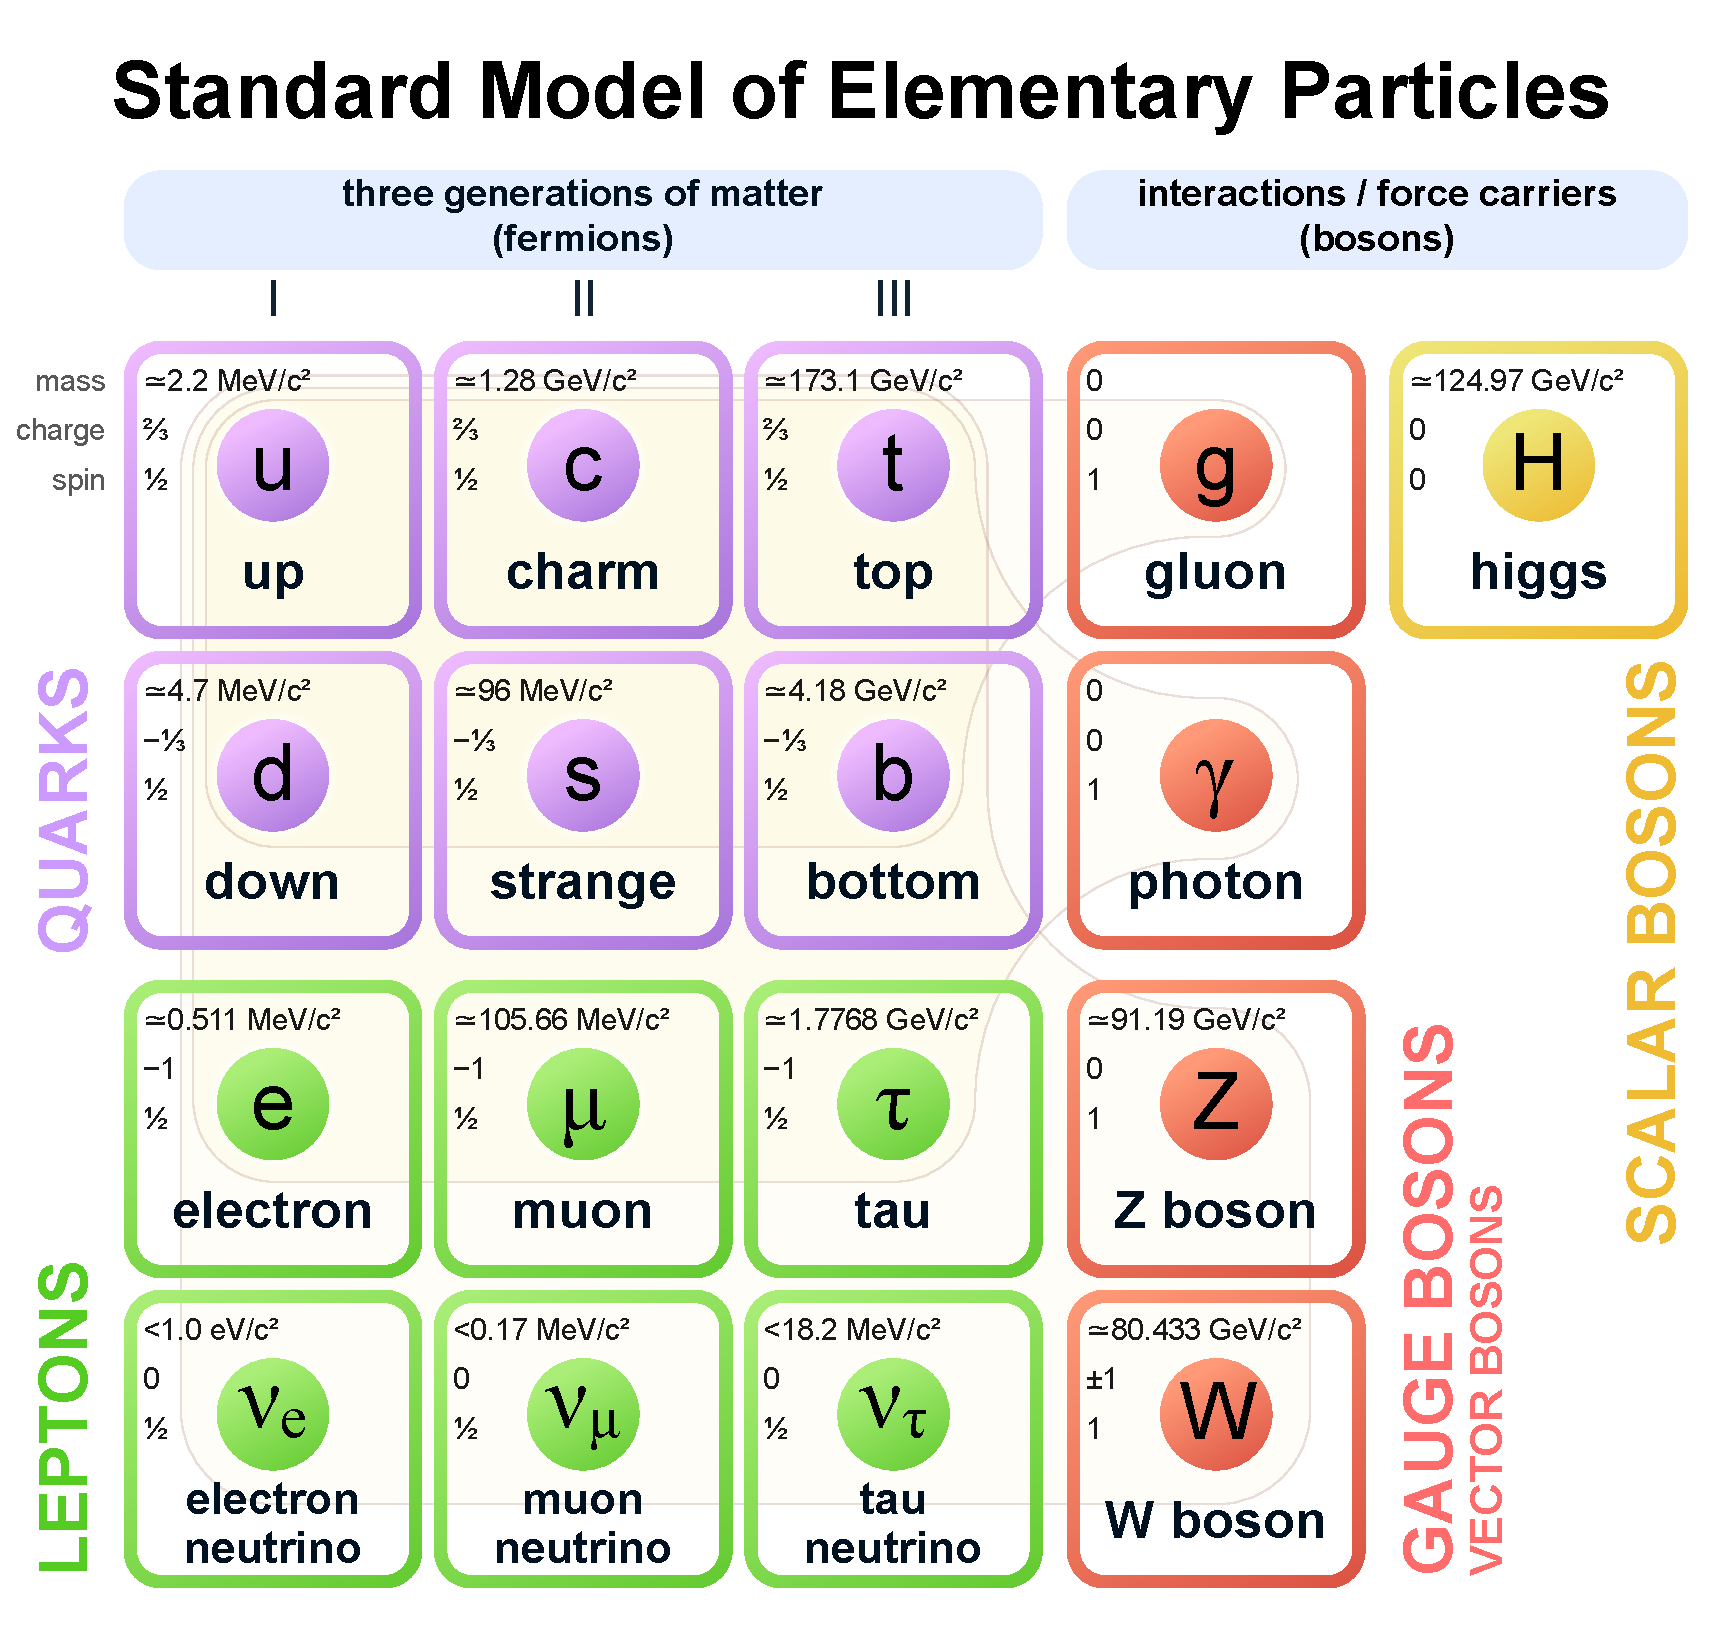
\includegraphics[width=0.9\textwidth]{fig_Theory/Standard_Model.pdf}
    \end{tabular}
    \caption{The Standard Model of Elementary Particle Physics
            }
    \label{Standard_Model}
  \end{center}
\end{figure}

\subsection{Fermions and Bosons}
In the SM, composite particles of matter are described in terms of their constituent elementary particles of half-integer spin, called fermions, which are particles of matter which are bound together by the exchange of fundamental, force-carrying particles of integer spin, called bosons. 

Fermions are further categorized into subgroups of quarks and leptons.
Leptons and quarks carry electric charge ($Q$) and therefore participate in the electromagnetic interaction.
Quarks additionally carry red ($R$), green ($G$), or blue ($B$) color charge, and so can also participate in the strong interactions.
Because of this property and the nature of QCD, quarks cannot exist in isolation, but instead can only be observed confined to colorless bound states called hadrons.
There are three so-called generations of fermions, and each generation is composed of both a pair of leptons and a pair of quarks, resulting in a total of twelve fermions: six quarks and six leptons.
Fermions of higher generations are more massive than those of the previous generation.
The up ($u$) and down ($d$) quarks, together with the electron ($e$) and electron neutrino ($\nu_e$) leptons, compose the first generation of fermions.
Both protons and neutrons are composed of different combinations of three up and down quarks; therefore, virtually all atomic matter is composed of only first generation fermions.
The second generation of fermions consists of the charm ($c$) and strange ($s$) quarks as well as the muon ($\mu$) and muon neutrino ($\nu_\mu$) leptons.
Finally, the third generation of fermions is composed of the top ($t$) and bottom ($b$) quarks (sometimes nicknamed truth and beauty), together with the tau ($\tau$) and tau neutrino ($\nu_\tau$) leptons.
The $e$, $\mu$, and $\tau$, referred to as "charged leptons", carry $Q = -1$, but the $\nu_e$, $\nu_\mu$, and $\nu_\tau$ neutrinos are electrically neutral.
The $u$, $c$, and $t$ quarks, referred to as "up-type," carry $Q = +\frac{2}{3}$, whereas the $d$, $c$, and $b$ quarks, referred to as "down-type," carry $Q = -\frac{1}{3}$.
Left-handed quarks and leptons additionally carry weak isospin ($I$ with third component $I_3$) and therefore participate in the weak interaction.
Left-handed charged leptons and down-type quarks carry $I_3 = +\frac{1}{2}$, while left-handed neutrinos and up-type quarks $I_3 = -\frac{1}{2}$.
Every fermion, i.e. denoted arbitrarily as $x$, has an anti-matter counterpart denoted $\Bar{x}$, that has the same mass as $x$, but opposite-signed quantum numbers.
The opposite-signed inversions of red, green and blue color charges are anti-red, anti-green and anti-blue, respectively.

The fundamental interactions of the SM are described by exchange of mediating force-carrying spin-1 gauge bosons.
Mathematically, these mediators arise from the gauge field group generators of the symmetry groups $U(1)$, $SU(2)$, and $SU(3)$.
The SM also includes a spin-0 scalar boson that is associated with a scalar field responsible for breaking the weak isospin symmetry of the electroweak interaction.

\subsection{The Electromagnetic Interaction}
The photon ($\gamma$) is the massless and electrically neutral gauge boson that mediates the electromagnetic interaction between electrically charged particles.
The electromagnetic interaction is described by QED with gauge symmetry group $U(1)$.
The electromagnetic coupling, i.e. the fine structure constant $\alpha_{EM} \approx \frac{1}{137}$, is significantly small relative to unity.
For the given process, the momentum of mediating virtual photons depend on the square of the momentum transfer, and therefore the coupling constant "runs," and the interaction becomes stronger (but still significantly smaller than unity) at higher values of momentum transfer.
As $\alpha_{EM} << 1$ even at higher values of momentum transfer, perturbative power series expansions in $\alpha_{EM}$ have proven to be extremely effective at explaining experimental results with QED.
Despite only providing approximate predictions, this effectiveness has made QED one of the most well-tested and successful theories in physics.

\subsection{The Weak Interaction}
The $W^\pm$ and $Z$ are massive gauge bosons that mediate the weak interaction between fermions carrying weak isospin ($I$ with third component $I_3$).
$W^\pm$ carries $Q = 0$, while $Z$ is electrically neutral.
Weak isospins of $I_3 = \pm 1$ ($I_3 = 0$) are carried by the $W^\pm$ ($Z$) bosons.
The $W^\pm$ and $Z$ boson masses are $\sim \SI{80.4}{\GeV}$ and $\sim \SI{91.2}{\GeV}$ respectively, resulting in their lifetimes, $\sim \SI{e-25}{\s}$, being incredibly short.
The short lifetimes limit the interaction ranges to be extremely small scales, as the distance these bosons can travel before decaying is very short.
The weak interaction is responsible for fermionic decay processes, such as nuclear radioactivity, is the only fundamental interaction that violates parity ($P$), charge conjugation parity ($CP$), and time-reversal ($T$) symmetries, and is described in the SM by gauge symmetry group $SU(2)$.
$Z$ bosons mediate the neutral weak interaction between same-flavor fermions, while $W^\pm$ bosons mediate the charged weak interaction between leptons of the same generation and can also flavor mix quarks of different generations.
Information about the conversion probabilities of flavor changing weak decays for quarks is encoded in the parameters of the Cabibbo-Kobayashi-Maskawa (CKM) matrix.

\subsection{The Strong Interaction}
Gluons ($g$) are massless gauge bosons that mediate the strong interaction between color charged particles.
The strong interaction is described by QCD with gauge symmetry group $SU(3)_C$.
While quarks (anti-quarks) carry color (anti-color) charge, gluons uniquely carry both color and anti-color charge, and therefore, gluons can interact with other gluons at trilinear and quartic self-interaction vertices.
There is a color octet of 8 different types of gluons, corresponding to 8 independent color state superpositions of the $3^2$ color/anti-color combinations.
One additional independent state exists mathematically, a color singlet carrying no color charge, but there is no experimental evidence for it and $SU(3)_C$ does not allow it.

The strong coupling $\alpha_S$ runs vigorously as the momentum transfer decreases, i.e. the interaction strength between quarks becomes stronger the further they are separated from each other.
This property of QCD results in color confinement, because before the energy between two separated quarks becomes arbitrarily large, a critical energy is reached for hadronization, in which a new quark/anti-quark pair is materialized from the energy of the mediating gluon.
Hadrons are classified by the flavor combinations of their valence quarks, but because quark interactions are mediated by gluons that can interact with themselves and split into quark/anti-quark pairs, there also exists a sea of virtual quarks and gluons within hadrons.
Protons and neutrons, colorless flavor combinations of three valence quarks, are categorized as baryons, whereas colorless flavor combinations of one valence quark and one valence anti-quark, such as pions and kaons, are categorized as mesons.
Experimental evidence for colorless flavor combinations of five valence quarks, categorized as pentaquarks, and colorless flavor combinations of two valence quarks and 2 valence anti-quarks, have also been reported in recent years.
Of all known hadrons, only the proton appears to be stable; with a mean life time constrained to be at least $10^34$ years, proton decay has never been observed.

Another consequence of the running of $\alpha_S$ is asymptotic freedom.
At higher and higher values of momentum transfer, $\alpha_S$ asymptotically approaches zero, i.e. quarks and gluons behave more like free particles at high energies.
At sufficiently high values of momentum transfer, such as those in hard scattering processes at hadron collider experiments, perturbative power series expansions in $\alpha_S$ become effective at explaining experimental results with QCD.

\subsection{The GWS Model, EWSB, and the BEH Mechanism}
At low energy energies, the electromagnetic and weak interactions are distinctly separate forces.
For energy scales beyond the unification energy $\sim$\SI{246}{\GeV}, electroweak theory unifies these two interactions into a single force described by a spontaneously broken Yang-Mills field with gauge symmetry group $SU(2)_L \otimes U(1)_Y$, generated by weak isospin ($I$) and weak hypercharge ($Y$).
In the Glashow-Weinberg-Salam (GWS) mopde, the $U(1)_Y$ group is mediated by a massless $B^0$ boson via the weak hypercharge field, and the $SU(2)_L$ group is mediated by massless $W^1$, $W^2$, and $W^3$ bosons via the weak isospin fields.
The subscript $L$ indicates that only left-handed fermion doublets carry isospin, while the right-handed singlets do not.

In the SM, the $\gamma$, $Z$, and $W^\pm$ bosons arise from the Brout-Englert-Higgs (BEH) mechanism spontaneously inducing electroweak symmetry breaking (EWSB) in the GWS model.
Mathematically, electric charge $Q = I_3 + \frac{1}{2} Y$ arises as a specific linear combination of weak isospin and hypercharge.
Electrically neutral $\gamma$ and $Z$ bosons arise from mixed states of the $B^0$ and $W^3$ bosons:
\begin{align}
\left(\begin{array}{c}
\gamma \\
Z^0
\end{array}\right)=\left(\begin{array}{cc}
\cos \theta_{\mathrm{W}} & \sin \theta_{\mathrm{W}} \\
-\sin \theta_{\mathrm{W}} & \cos \theta_{\mathrm{W}}
\end{array}\right)\left(\begin{array}{c}
B \\
W_3
\end{array}\right)
\label{}
\end{align}
where $\theta_{\mathrm{W}}$ is the Weinberg weak mixing angle.
Electrically charged $W^\pm$ bosons arise from linear combinations of the $W^1$ and $W^2$ bosons:
\begin{align}
W^{\pm}=\frac{1}{\sqrt{2}}\left(W_1 \mp i W_2\right).
\label{}
\end{align}

In the GWS model, local gauge symmetry prohibits mass terms in the Lagrangian for gauge bosons (Goldstone's theorem), but the $W^\pm$ and $Z$ bosons are experimentally known to have large masses.
To both resolve this discrepancy and induce EWSB, the BEH mechanism adds a complex scalar $SU(2)$ doublet field $\phi$ to the SM that permeates all of space:
\begin{align}
\phi=\left(\begin{array}{l}
\phi^{+} \\
\phi^0
\end{array}\right)=\frac{1}{\sqrt{2}}\left(\begin{array}{l}
\phi_1+i \phi_2 \\
\phi_3+i \phi_4
\end{array}\right)
\end{align}
with potential energy:
\begin{align}
V(\phi) = -\mu^2 \phi^{\dagger} \phi + \lambda\left(\phi^{\dagger} \phi\right)^2
\end{align}
The BEH potential, colloquially referred to as a Mexican-hat potential, has global $U(1)$ and $SU(2)$ symmetries.
The energy at the center of the potential is higher than at a ring of equivalent vacuum states with vacuum expectation energy $\langle\phi\rangle=\sqrt{\frac{\mu^2}{2 \lambda}} \equiv \frac{v}{\sqrt{2}}$ that breaks the electroweak gauge symmetry.
Without loss of generality, $\phi$ can be parameterized with an expansion around $v$, by introducing scalar field $h$, and with a unitary gauge transformation:
\begin{align}
\phi=\frac{1}{\sqrt{2}}\left(\begin{array}{c}
0 \\
v+h
\end{array}\right)
\end{align}
Of the original four degrees of freedom in the complex scalar $SU(2)$ doublet field, the electrically charged $\phi_1$ and $\phi_2$ are absorbed to generate mass terms in the Lagrangian for the $W^\pm$ bosons, while the electrically neutral $\phi_4$ term is absorbed to generate mass for the $Z$ boson.
The remaining electrically neutral $\phi_3$ is split into $v$ and the new field $h$, with quantum numbers $I_3 = \frac{-1}{2}$ and $Y = +1$ ($Q = 0$), which manifests as the physical Higgs ($H$) boson, a scalar boson that mediates interactions between the fermions and the BEH field, endowing them with mass proportional their Yukawa coupling constant $y_f$.
The Higgs boson was experimentally discovered in 2012 jointly by the CMS and ATLAS LHC experiments at CERN; Peter Higgs and François Englert received the 2013 Nobel Prize in Physics for their theoretical predictions, while Robert Brout passed away in 2011.

\section{Beyond the Standard Model}
The SM is a central pillar of modern particle physics, many of its predictions have been confirmed by innumerable experiments to exquisite precision, and is considered to be one of the most mature and successful theories in all of science.
Despite its success, there are a number of known physical phenomena that are not explained by the SM, and it is considered to be an effective theory up to some scale $\Lambda \approx \si{\TeV}$.
All theoretical and experimental investigations that are beyond the current understanding of the Standard Model of particle physics are collectively referred to as Beyond the Standard Model (BSM).

Following the example of electroweak unification, theoretical frameworks that aim to unify the strong and electroweak interactions into a single, unified force are referred to as Grand Unification Theories (GUT).
While the scale of electroweak unification is $\sim \SI{e2}{\GeV}$, the scale of grand unification is estimated to be $\sim \SI{e14}{\GeV} - \SI{e16}{\GeV}$.
Given the extreme energy requirements, it is unsurprising that no experimental evidence for GUT predictions have been found yet at energy scales accessible to modern particle accelerator experiments.

The the theoretical explanation for the experimental observation of neutrino oscillations predicts that the neutrino masses are non-zero.
However. the SM predicts that neutrinos should be massless particles. 

The discovery of the Higgs boson with mass $\sim \SI{125}{\GeV}$ has creating an inconsistency in the SM known as the "Heirarchy Problem."
Virtual loop corrections to the Higgs boson mass generate quadratic divergences.
Calculating a predicted Higgs boson mass compatible with the observed value requires unnatural fine-tuning, highlighting the likelihood of New Physics (NP) between the electroweak scale and the Planck scale, natural scale of quantum gravity.

The most glaring absence from the SM framework is the gravitational interaction between massive objects.
A theory that reduces all four physical interactions into a single, unified theory is colloquially referred to as the "Theory of Everything," and it is the holy grail of particle physics.
Einstein's general theory of relativity (GR) is a classical theory of gravitation that describes the force of gravity as resulting from the curvature of spacetime caused by the presence of massive objects.
All attempts to unify the SM and GR have failed, and the two are considered to be separate and incompatible theories.
A major focus of current theoretical physics research is centered around the formulation of a QFT that describes the gravitational interaction, but a common feature of these theories is that they are non-renormalizable.
Theories of quantum gravity predict the existence of a massless, spin-2 gauge boson dubbed the graviton.
Experimentally however, gravity is $\sim 10^{24}$ times weaker than the weak interaction, and the lack of experimental sensitivity makes it extremely difficult to verify the predictions of these theories.

There are astrophysical and cosmological observed physical phenomena as well that are not explained by the SM.
The asymmetry between the observed matter and anti-matter in the universe remains unexplained by the SM.
Based on the assumption that the universe started with equal quantities of matter and anti-matter, the conditions required for baryogenesis, i.e. the generation of a cosmological excess of baryons over anti-baryons, include baryon number violation, CP-violation, and charge conjugation symmetry ($C$) violation.
Sources of CP-violation in the SM via the weak interaction are not sufficient to account for the extreme asymmetry and baryon number is not violated whatsoever.
CP-violation via the strong interaction is mathematically allowed in the SM, but the relevant parameters have been inexplicably measured to be extremely small (strong CP problem).
Astronomical observations of gravitational lensing effects and in the velocity of rotation curves of spiral galaxies suggest that $85 \%$ of all observed matter in the universe is dark matter, an unknown form of matter that has its namesake in that it does not emit, absorb or reflect electromagnetic radiation, and thus can only be indirectly inferred through its gravitational effects on visible matter.
Although dedicated dark matter detection experiments exist that search for Weakly Interacting Massive Particles (WIMP), conclusive direct observation of dark matter WIMPs has not yet occurred.
Cosmological observations of galaxies also indicate that the expansion of space is accelerating.
The cause of this expansion is unknown, but it is attributed to an enigmatic form of energy, dubbed dark energy, that is thought to be responsible for $73 \%$ of the total energy density of the universe.

Many BSM extensions have been made that predict new elementary particles that, depending on their properties and stability, could explain dark matter.
Perhaps the most popular of these extensions is Supersymmetry (SUSY), which predicts the existence of superpartners for every fermion and boson in the SM by adding terms to the Lagrangian and make it symmetric with respect to matter and field-mediating particles.
SUSY can resolve the hierarchy problem by providing superpartner terms that cancel the quadratic divergences to the Higgs boson mass from heavy virtual particles.
Despite compelling arguments for why the predicted superpartners could be in reach of LHC experiments, the lack of experimental evidence for SUSY has led to a resurgence of interest in alternative BSM models to resolve these open questions.

SM Effective Field Theory (SMEFT) is a model-independent extension of the Standard Model which uses a systematic product expansion in terms of higher-dimensional operators to describe the effects of NP at higher energy scales.  
Due to its agnostic construction, SMEFT allows for a broad range of possibilities for NP, which is parameterized as coefficients of the operators in the expansion, referred to as Wilson coefficients.


\ProvidesFile{chapters/ch-LHC_CMS.tex}

\chapter{THE COMPACT MUON EXPERIMENT AT THE LARGE HADRON COLLIDER}
\label{The_CMS_Experiment_at_the_LHC}

\section{The Large Hadron Collider}
Experiments to discover and determine the properties of SM particles are performed at particle accelerator facilities.
The Large Hadron Collider (LHC) is a $\SI{27}{\km}$ circular particle accelerator located at the European Center for Nuclear Research (CERN) designed to accelerate two counter-rotating proton beams to energies up to $\SI{6.8}{\TeV}$ ($99.999999\%$ the speed of light) and collide them at designated interaction points (IP).
The LHC is the largest and most powerful particle accelerator ever built; its design, construction, and operation are towering engineering achievements of mankind, requiring an international collaboration of thousands of scientists, engineers, and technicians from more than 100 countries.
The successful operation of the LHC has contributed to our understanding of the fundamental nature of matter by providing conditions to test the hypotheses of the SM and enabling many important discoveries in particle physics.
The primary design criteria for the LHC were to provide conditions for elucidating the nature of EWSB, testing the hypothesis of the BEH mechanism, and discovering the Higgs boson.

\subsection{Probing Small Scales with High Energy}
The De Broglie relation states that the wavelength of a particle is inversely proportional to its energy.
According to Heisenberg's uncertainty principle, the position of a particle with a short wavelength cannot be precisely determined.
Thus, the motivation for building higher energy particle colliders is to probe smaller distance scales.
In the 20th century, particle accelerator energy increased many orders of magnitude from \sim$\SI{100}{\keV}$ in the 1930s to \sim$\SI{10}{\TeV}$ in the 2010s (see table~\ref{energy_distanceprobed}), and current distance scales probed are down to \sim$\SI{e-19}{\m}$.
\begin{table}[htb]
\begin{center}
\begin{math}
\begin{array}{|c|c|c|}
\hline \text { Decade } & \text { Energy } & \text { Distance Probed } \\
\hline 1930 & \sim \SI{100}{\keV} & \sim \SI{e-11}{\m} \\
\hline 1950 & \sim \SI{100}{\MeV} & \sim \SI{e-14}{\m} \\
\hline 1970 & \sim \SI{100}{\GeV} & \sim \SI{e-17}{\m} \\
\hline 1990 & \sim \SI{1}{\TeV} & \sim \SI{e-18}{\m} \\
\hline 2010 & \sim \SI{10}{\TeV} & \sim \SI{e-19}{\m} \\
\hline
\end{array}
\end{math}
\caption{In the 20th century, particle accelerator energy increased many orders of magnitude from \sim$\SI{100}{\keV}$ in the 1930s to \sim$\SI{10}{\TeV}$ in the 2010s, and current distance scales probed are down to \sim$\SI{e-19}{\m}$.
        }
\label{energy_distanceprobed}
\end{center}
\end{table}

\subsection{Accelerator Complex at CERN}
Before reaching the LHC, protons must be accelerated through a series of smaller accelerators at CERN's accelerator complex.
A schematic of the LHC at CERN's accelerator complex in Geneva at the border of Switzerland and France is shown in figure~\ref{CERN_LHC}.
\begin{figure}[htb]
  \begin{center}
    \begin{tabular}{c}
        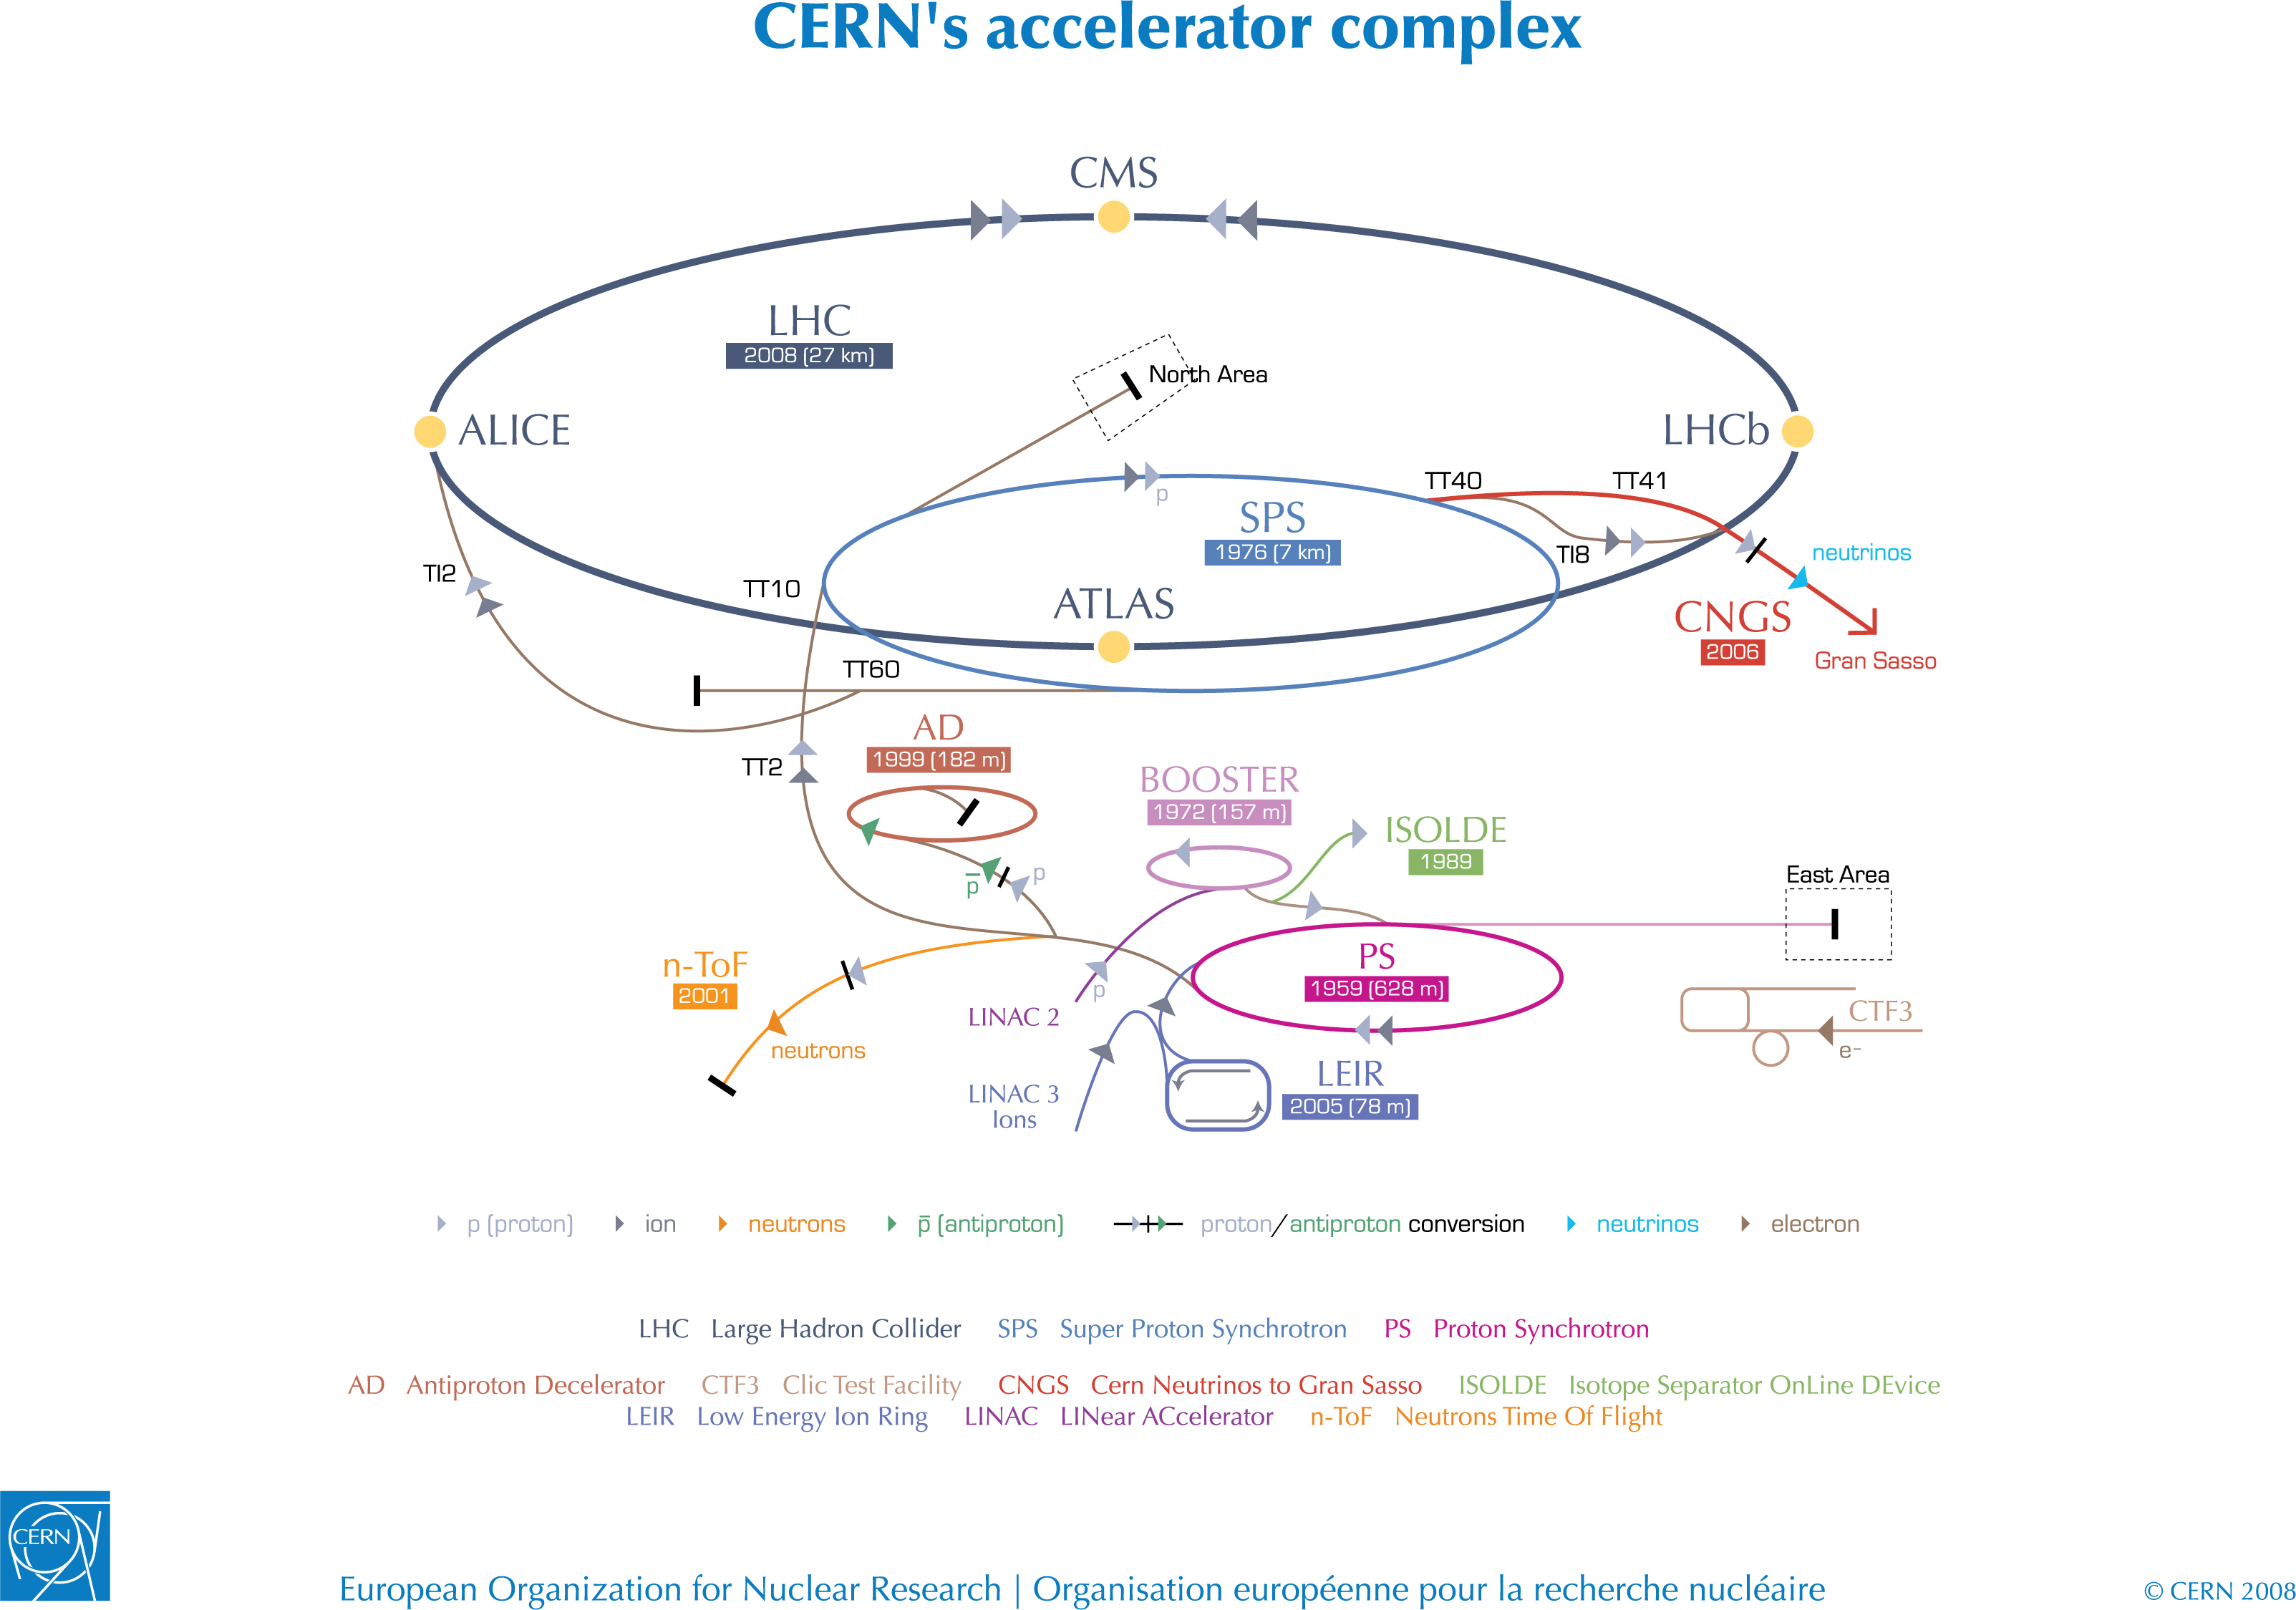
\includegraphics[width=0.9\textwidth]{fig_LHC_CMS/CERN_LHC.png}
    \end{tabular}
    \caption{A schematic of the LHC at CERN's accelerator complex in Geneva at the border of Switzerland and France~\cite{Christiane:1260465}.
            }
    \label{CERN_LHC}
  \end{center}
\end{figure}
Protons are produced from hydrogen gas by inducing electric discharge in a duoplasmatron.
The $\SI{80}{\m}$ Linear Accelerator 2 (Linac 2) accelerates protons to an energy of $\SI{160}{\MeV}$ before injecting them into the $\SI{157}{\m}$ circumference Proton Synchrotron Booster (PSB), which divides the beam into bunches consisting of more than 100 billion protons with $\SI{25}{\ns}$ separation, and further increases the proton energy to $\SI{2}{\GeV}$.
Next, the proton bunches are injected into the $\SI{628}{\m}$ circumference Proton Synchrotron (PS), which accelerates the bunches to $\SI{26}{\GeV}$ before injecting them into the $\SI{7}{\km}$ circumference Super Proton Synchrotron (SPS), which increases the proton energy to $\SI{450}{\GeV}$ before finally injecting them into the LHC, which accelerates them to their final (2016, 2017, and 2018) energy of $\SI{6.5}{\TeV}$.

Ultra-high vacuum conditions \sim$\SI{e-11}{\mbar}$ are maintained in the LHC beam pipes and 16 radiofrequency (RF) cavities with electric fields oscillating at a frequency resonant with the bunching frequency are used to accelerate the protons.
Superconducting magnets cooled with superfluid helium to temperatures below $\SI{2}{\K}$ and operating at fields exceeding $\SI{8}{\T}$~\cite{LyndonEvans_2008} are used to shape and control the beam directions.
1232 dipole magnets bend the beams around the ring and 474 quadrupole magnets are used to focus and collimate the beams.
The $\SI{25}{\ns}$ bunch separation corresponds to 2808 proton bunches simultaneously in the LHC.
At the four LHC IPs, proton bunches cross at a rate of $\SI{40}{\MHz}$, creating collisions corresponding to temperatures a billion times hotter than the core of the sun.
Final states after the collisions are measured and recorded by the CMS, ATLAS, ALICE, and LHCb particle detectors.

\subsection{Luminosity}
When two particle beams cross paths in a particle accelerator, the number of events of a particular process that occur per second is given by:
\begin{linenomath*}
\begin{align}
{\frac{dN_{\text {Events}}}{dt}}= \mathcal{L}_{\text{Inst}} \cdot \sigma_{\text{Process}}
\end{align}
\end{linenomath*}
where $\mathcal{L}_{inst}$ is the instantaneous luminosity and $\sigma_{\text{Process}}$ is the cross-section of the process under consideration.
For the \beamenergy LHC, the total cross-section for all inelastic processes has been measured to be $\sigma_{\text{Inelastic}} = 68.6 \pm 0.5 \; (\text{Syst}) \; \pm 1.6 \; (\text{Lumi}) \; \si{\milli \b}$~\cite{inelasticprotonprotoncrosssection}.
The instantaneous luminosity can be parameterized~\cite{Karacheban:2294183} as:
\begin{linenomath*}
\begin{align}
\mathcal{L}_{\text{Inst}}=\frac{N_b^2 n_b f_{\mathrm{rev}}}{A_{eff}}
\end{align}
\end{linenomath*}
where $N_b = \num{1.15e11}$ is the number of particles per bunch, $n_b=2808$ the number of bunches per beam, $f_{\mathrm{rev}} = \SI{11245}{\Hz}$ the revolution frequency in the collider, and $A_{eff} = \sqrt{\varepsilon_x \beta_x \varepsilon_y \beta_y}$ is the effective area of the luminous region, where $\beta_{x,y}$ and $\varepsilon_{x,y}$ are the beam amplitude and emittance transverse to the beam axis, and is measured regularly during Van der Meer (VdM) scans.
$\mathcal{L}_{\text{Inst}}$ decays over time due to the intensity degradation and beam emittance, with a mean life of \sim$\SI{15}{\h}$~\cite{LyndonEvans_2008}.
The high $\mathcal{L}_{\text{Inst}}$ of the LHC typically results in many proton-proton interactions per bunch crossing.
The number of collisions per bunch cross is referred to as pile-up (PU), and is quantified as:
\begin{linenomath*}
\begin{align}
PU = \frac{\mathcal{L}_{\text{Inst}} \cdot \sigma_{\text{Inelastic}}}{n_b f_{\mathrm{rev}}}
\end{align}
\end{linenomath*}
where $\sigma_{\text{Inelastic}} = \SI{69.2}{\milli \b}$ is the total $pp$ inelastic cross section at the \beamenergy LHC.
Typical PU in CMS recorded data from 2016 through 2018 was around 15-30 interaction vertices per bunch crossing, but high (low) extremes routinely occurred during the beginning (end) of beam fills due to instantaneous luminosity decay.
For a particular process, the total number of events that occur in a recorded data set is given by:
\begin{linenomath*}
\begin{align}
N_{\text {Events}}= \mathcal{L} \cdot \sigma_{\text{Process}}
\end{align}
\end{linenomath*}
where the integrated luminosity $\mathcal{L} = \int \mathcal{L}_{\text{Inst}} \,dt$ is the instantaneous luminosity integrated over the corresponding periods of time the data was recorded.

\subsection{Upcoming High Luminosity - LHC Phase}
During 2016, 2017, and 2018, the LHC operated with beam energies of $\SI{6.5}{\TeV}$, corresponding to center-of-mass collision energies of $\SI{13}{\TeV}$.
Recently, the LHC finished upgrading the beam energies to $\SI{6.8}{\TeV}$.
After operating at $\sqrt{s}=\SI{13.6}{\TeV}$ through 2025, the LHC plans to vastly increase the instantaneous luminosity, and substantial R\&D effort is underway to prepare accelerator and detector upgrades for high luminosity (HL-LHC) environments.

\section{The Compact Muon Solenoid Detector}
Particle detectors measure electrical signals and collect scintillated light produced by particles interacting with the material of the detector.
The Compact Muon Solenoid (CMS) is a general-purpose detector, built for testing predictions of the SM, exploring models BSM, and discovering NP.
The primary design benchmarks for CMS were precision studies of QCD, electroweak, and flavor physics, as well as the detection of the Higgs boson.
CMS is a collection of sub-detectors that are layered cylindrically around the IP, with barrel and end-cap/disk components, that provide the detector with near-hermetic coverage of the solid angle.
An exploded view of the CMS detector layout with labeled sub-detectors is shown in figure~\ref{CMS_Detector}.
\begin{figure}[htb]
  \begin{center}
    \begin{tabular}{c}
        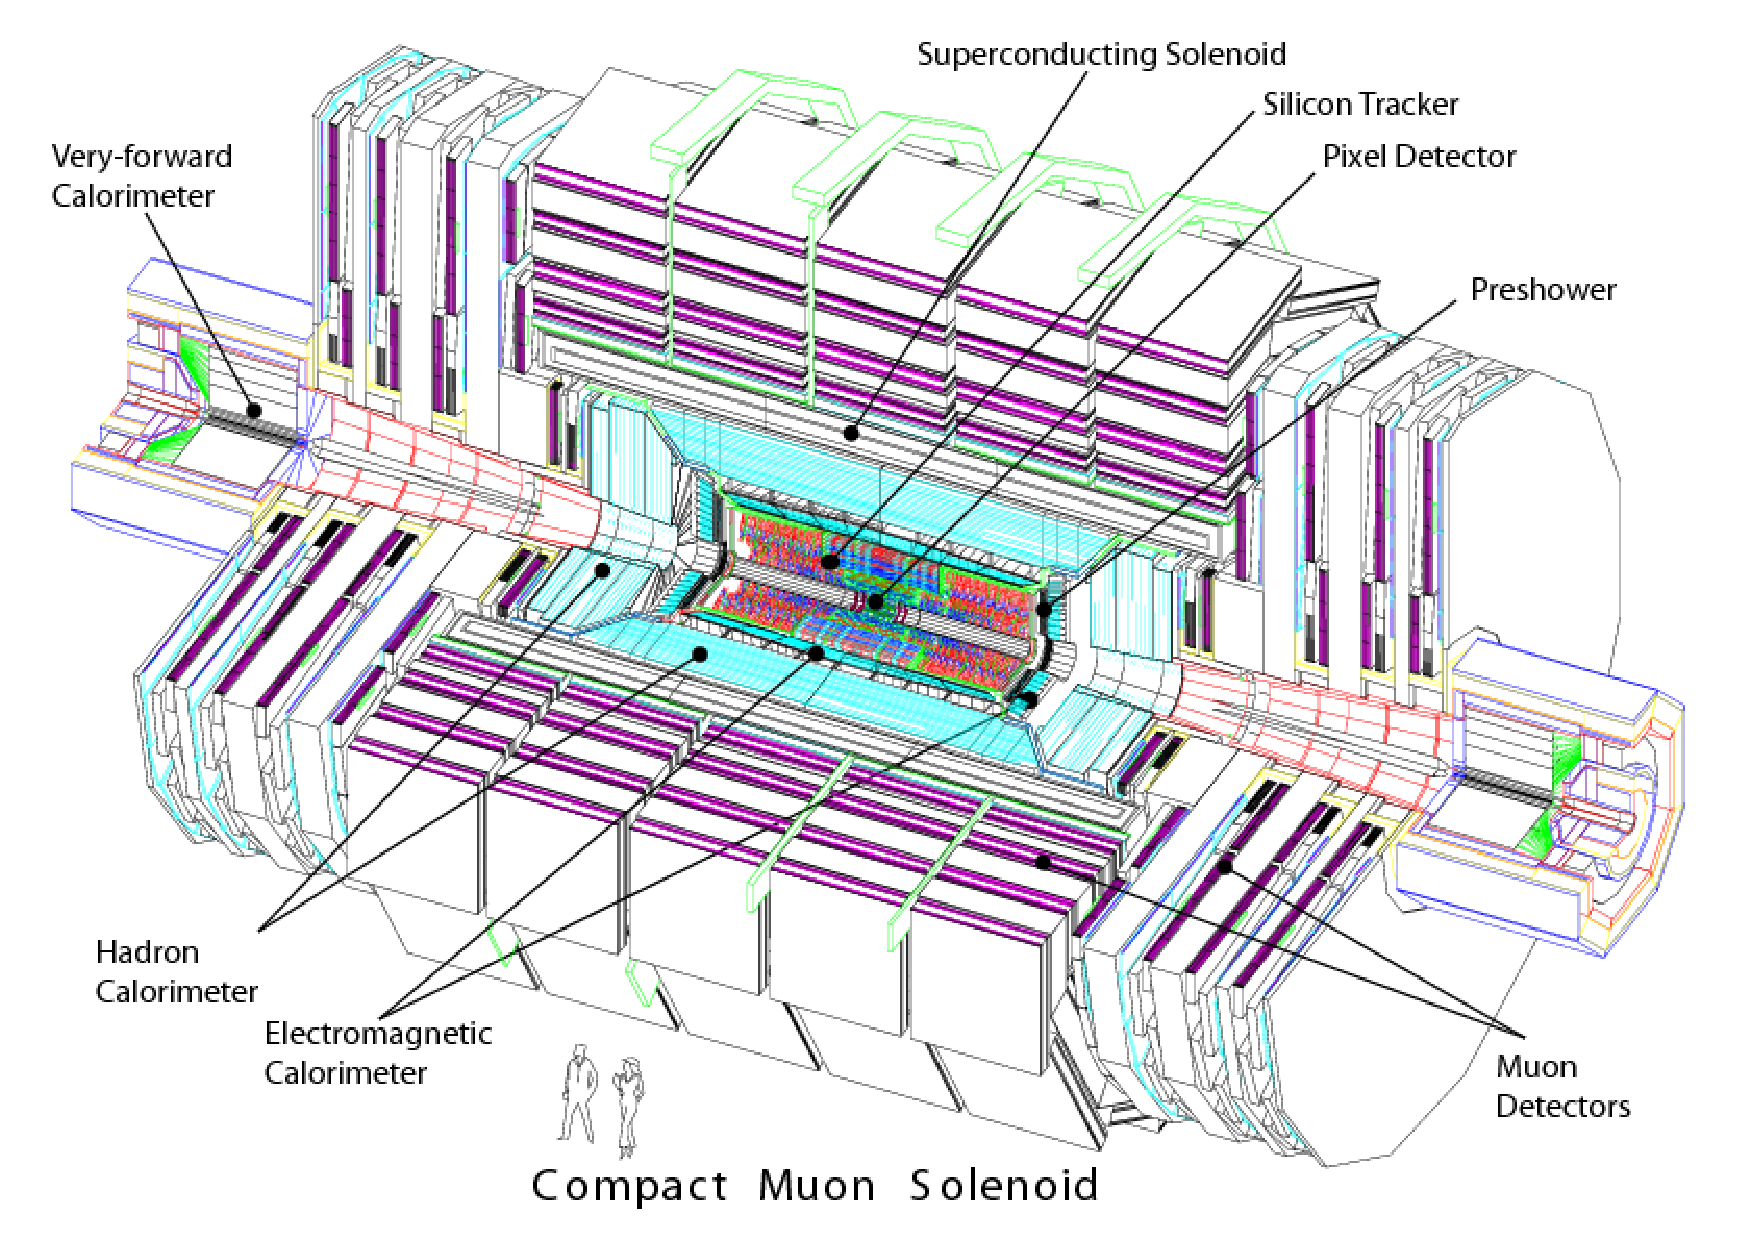
\includegraphics[width=0.9\textwidth]{fig_LHC_CMS/CMS_Detector.pdf}
    \end{tabular}
    \caption{An exploded view of the CMS detector layout with labeled sub-detectors~\cite{Bayatian:922757}.
            The human figures are included for scale.
            }
    \label{CMS_Detector}
  \end{center}
\end{figure}
Overall, the CMS detector is $\SI{21.6}{\m}$ long, with a diameter of $\SI{14.6}{\m}$, and weighs more than $\SI{12500}{\t}$.

\subsection{Coordinate System}
\label{CMS_Coordinate_System}
The CMS origin is located at the nominal interaction point of the beams at the center of the experiment.
The $\hat{y}$-axis points vertically upward, the $\hat{z}$-axis is along the beamline, and the $\hat{x}$-axis points towards the center of the LHC ring.
When analyzing the kinematics of high-energy particle collisions, it is more conventional to use the $\pT$, $\eta$, $\phi$ coordinate system:
\begin{itemize}
\item The transverse momentum $\pT = \sqrt {{p_x}^2+{p_y}^2}$ is the momentum component of a particle perpendicular to the beam axis. 
\item The pseudorapidity $\eta$ is a measure of the angle between the particle's momentum vector and the beam axis.
Pseudorapidity is defined as: 
\begin{linenomath*}
\begin{align}
\eta=\frac{1}{2} \ln \frac{\vert\vec{p}\vert+p_z}{\vert\vec{p}\vert-p_z}=-\ln \left[\tan \left(\frac{\theta}{2}\right)\right]
\end{align}
\end{linenomath*}
in terms of the polar angle $\theta$, which is measured from the z-axis.
For particles with $m {{\ll}\!\!\!\!/} \; \vert \vec{p} \vert$, it is sometimes preferable to use rapidity, defined as:
\begin{linenomath*}
\begin{align}
y=\frac{1}{2} \ln \frac{E+p_z}{E-p_z}
\label{Rapidity}
\end{align}
\end{linenomath*}
which converges to pseudorapidity in the ultra-relativistic limit.
One advantage of using pseudorapidity (rapidity) is that differences in $\eta$ ($y$) are Lorentz invariant for longitudinal Lorentz boosts along the beam axis.
\item The azimuthal angle $\phi$ is the angle in the transverse plane between the particle's momentum vector and the $\hat{x}$-axis.
\end{itemize}
The energy $E$ of a particle, together with its 3-vector $\langle \pT, \eta, \phi \rangle$, form a 4-vector $(E,\pT, \eta, \phi)$ that fully characterizes the particle's momentum and energy in space and time.

A measure of angular separation between objects $i$ and $j$ can be defined using $\eta$ and $\phi$ coordinates:
\begin{linenomath*}
\begin{align}
\Delta R_{ij} = \sqrt {{(\phi_i - \phi_j)}^2+{(\eta_i - \eta_j)}^2};
\label{DeltaR}
\end{align}
\end{linenomath*}
this quantity is useful for clustering particle showers into jets and rejecting events with overlapping objects.

\subsection{Solenoid Magnet}
Central to the design of the CMS detector, and the source of its name, is the $\SI{12.9}{\m}$-long, $\SI{5.9}{\m}$ inner diameter, $\SI{200}{\t}$, niobium-titanium alloy superconducting solenoid, providing an axial and uniform $\SI{3.8}{\T}$ magnetic field within the solenoid, and a return field outside the solenoid that is confined by an iron yoke that contains and guides the field.
The solenoid is large enough that the inner tracking detectors and calorimeters fit inside, which advantageously eliminates energy losses caused by showering in the coil material before energy can be measured in the calorimeters.
The magnetic field of the solenoid, depicted in figure~\ref{Solenoid}, bends the paths of charged particles as they move through the detector, enabling the tracker to make good resolution measurements of their transverse momentum and charge from their curvature.
\begin{figure}[htb]
  \begin{center}
    \begin{tabular}{c}
        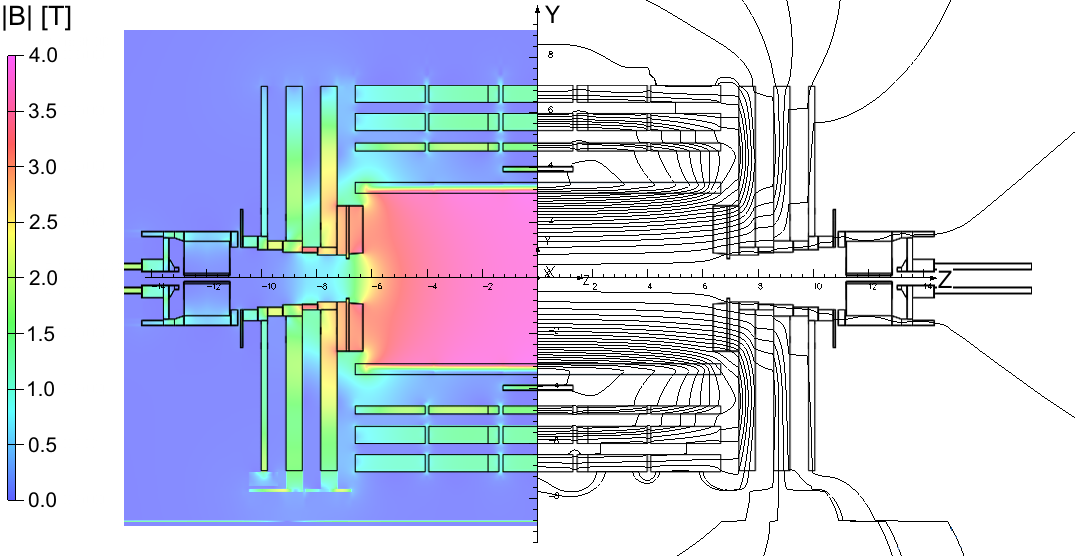
\includegraphics[width=0.65\textwidth]{fig_LHC_CMS/Solenoid.png}
    \end{tabular}
    \caption{Magnitude of magnetic field (Left) and field lines (Right) simulated on a longitudinal section of the CMS detector~\cite{Chatrchyan:1215500}.
            }
    \label{Solenoid}
  \end{center}
\end{figure}


\subsection{Silicon Inner Tracker}
The inner tracker consists of silicon pixel detectors surrounded by silicon strip detectors.
Silicon detector technology provides high granularity, fast response, radiation hardness, and efficient cooling, while also minimizing material to limit multiple scattering, bremsstrahlung, photon conversion, and nuclear interactions.
High-energy charged particles ionize the silicon as they traverse the detectors, leaving trails of position measurements that are used to reconstruct the particle trajectories with sophisticated algorithms.
The magnetic field of the solenoid exerts a force perpendicular to a charged particle's transverse momentum, and transverse momentum magnitude is measured from the curvature of its trajectory.
The inner tracker cylindrical volume of length $\SI{5.8}{\m}$ and diameter $\SI{2.6}{\m}$ covers out to $\vert \eta \vert < 2.5$ and is separated into the barrel and forward regions.

The silicon pixel tracker operates closest to the IP, in the region with the highest radiation and particle flux from the $pp$ collisions.
The primary limiting factor for impact parameter resolution is the radial distance of the innermost tracking layer.
In the barrel region, three layers of pixel detectors, $\SI{53}{\cm}$ long, are at radial distances $r = 4.4, 7.3, 10.2 \si{\cm}$ from the beam, while in the forward regions, two end-cap disks with radii $\SI{6}{\cm}$ and $\SI{15}{\cm}$ are placed on each side at $z = \pm \SI{34.5}{\cm}$ and $\SI{46.5}{\cm}$.
The doping scheme for the pixels is $n$-on-$n$, which can be operated partially depleted even at high fluence.
To minimize occupancy in the inner region of high particle flux and achieve good vertex resolution for the identification of primary and secondary vertices, pixel detectors are highly granular and finely segmented in two dimensions with pixel size $\approx 100 \times 150 \; \mu \si{\m \squared}$.
The pixel detector consists of 1440 modules that cover a total area of $\approx \SI{1}{\m \squared}$, so altogether it contains about 66 million pixels.
In the barrel region, $r-\phi$ resolution is improved through charge-sharing among pixels due to the Lorentz effect, while in the forward region, modules are rotated in a turbine-like geometry to improve the resolution by inducing charge-sharing.
The spatial resolution of the pixel detector is $10 \; \mu \si{\m}$ ($20 \; \mu \si{\m}$) for $r-\phi$ ($z$) measurements.

During the LHC winter shutdown between 2016 and 2017, the entire pixel tracker was replaced (see figure~\ref{Inner_Tracker}) with the Phase-1 upgrade~\cite{Lipinski_2017}.
A fourth layer was added in the barrel region, and the radius of the innermost layer was reduced from $r = \SI{4.4}{\cm}$ to $r = \SI{2.9}{\cm}$, a fifth layer was added in the forward regions, and the total number of pixels increased to 124 million.
The cooling system was replaced with evaporative \ce{CO2} cooling technology, which utilizes the latent heat of vaporization to efficiently remove heat.
After the replacement, the silicon inner tracker altogether contributes total radiation length up to \sim$0.5 X_0$ and total interaction length up to \sim$1.8 \lambda_I$, mostly from supports, cables, and cooling~\cite{Sirunyan:2270046}.
\begin{figure}[htb]
  \begin{center}
    \begin{tabular}{cc}
        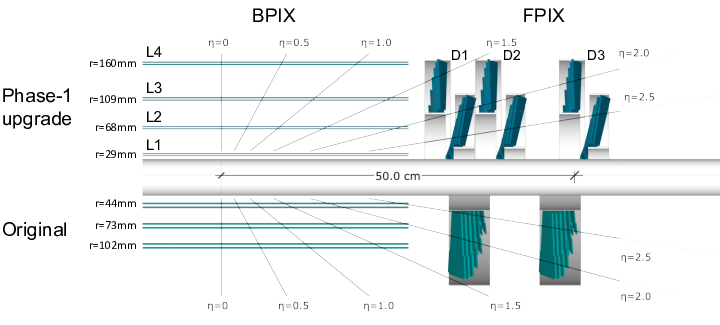
\includegraphics[width=0.45\textwidth]{fig_LHC_CMS/Pixel_Upgrade.png}
        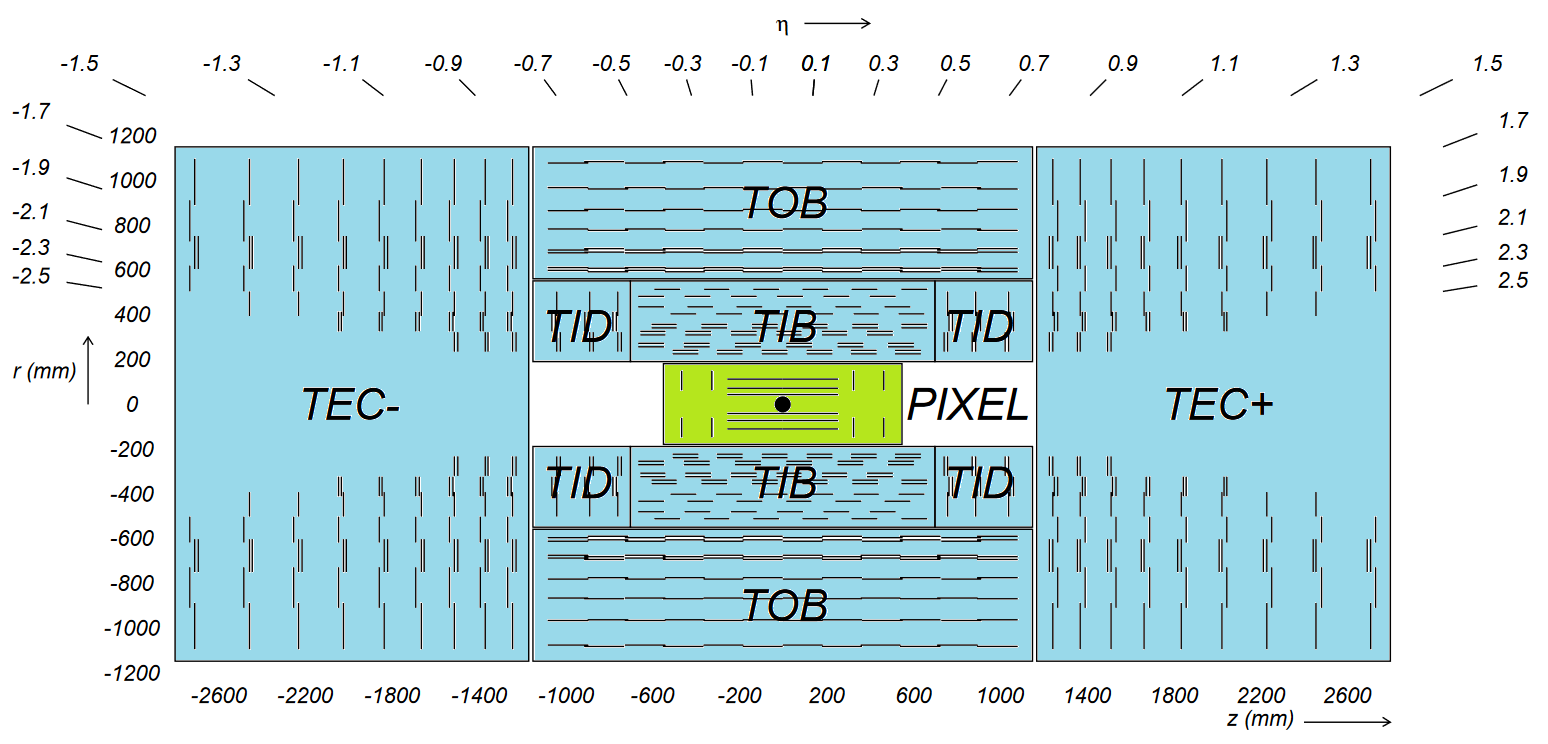
\includegraphics[width=0.45\textwidth]{fig_LHC_CMS/Inner_Tracker.png}
    \end{tabular}
    \caption{Silicon Pixel Tracker (Left) before and after the Phase-1 upgrade~\cite{Adam_2021}.
             Silicon Inner Tracker before Pixel Phase-1 upgrade (Right): ~\cite{Chatrchyan:1211825}.
            }
    \label{Inner_Tracker}
  \end{center}
\end{figure}

Surrounding the pixel tracker is the silicon strip tracker (see figure~\ref{Inner_Tracker}), consisting of 15,148 modules with 24,244 silicon sensors, that cover a total area of $\approx \SI{198}{\m \squared}$, and altogether contains 9.6 million microstrips.
In the barrel region, the strip tracker is separated into the Tracker Inner Barrel (TIB), which covers from $\SI{20}{\cm} < r < \SI{55}{\cm}$ out to $z = \pm \SI{65}{\cm}$, and the Tracker Outer Barrel (TOB), which covers from $\SI{55}{\cm} < r < \SI{116}{\cm}$ out to $z = \pm \SI{118}{\cm}$.
In the forward regions, the strip tracker is separated into the Tracker Inner Disks (TID$^\pm$), which cover $\pm\SI{65}{\cm} < z < \pm\SI{124}{\cm}$ and $\SI{20}{\cm} < r < \SI{55}{\cm}$, and Tracker End-Caps (TEC$^\pm$), which cover $\pm\SI{124}{\cm} < z < \pm\SI{282}{\cm}$ and $\SI{22.5}{\cm} < r < \SI{113.5}{\cm}$.
The doping scheme for strips is $p$-on-$n$, which undergoes type inversion after sufficient radiation damage to the crystal lattice and change.
Strips are only finely segmented in one dimension, with minimum cell sizes of  $\approx \SI{10}{\cm} \times 80 \; \mu \si{\m}$ in the TIB and TID, and maximum cell sizes of $\approx \SI{25}{\cm} \times 180 \; \mu \si{\m}$ in the TOB and TEC.
The TIB (TOB) has four (six) layers of silicon microstrip detectors, providing up to four (six) $r-\phi$ measurements, while the TID (TEC) has four (nine) layers, providing up to four (nine) $z-\phi$ measurements.
The $r\-phi$ ($z$) single point resolutions of these measurements are $23-35 \; \mu \si{\m}$ ($23 \; \mu \si{\m}$) in the TIB, $35-52 \; \mu \si{\m}$ ($52 \; \mu \si{\m}$) in the TOB.
Some layers additionally have modules mounted with stereo angles to provide measurements of the second coordinate ($z$ in the barrel region and $r$ in the forward regions).
The single point resolutions of these measurements are $\approx 230 \; \mu \si{\m}$ in the TIB, $\approx 530 \; \mu \si{\m}$ in the TOB.
The hit efficiency of the silicon strip tracker is 99.8\%.

\subsection{Electromagnetic Calorimeter}
Surrounding the silicon inner tracker is the electromagnetic calorimeter (ECAL), consisting of 61,200 lead tungstate (\ce{PbWO4}) scintillating crystals in the barrel region (EB) and 7,324 crystals in each of the end-caps (EC).
The EB covers out to $\vert \eta \vert < 1.479$, with inner radius $\SI{1.29}{\m}$, while the EE covers $1.479 < \vert \eta \vert < 3.0$, at a longitudinal distance $\vert z \vert = \SI{3.15}{\m}$ from the IP (see figure~\ref{ECAL_HCAL}).

The ECAL measures the energy of particles, such as electrons, positrons, and photons, that primarily interact electromagnetically.
Lead tungstate is high density $\SI{8.28}{\g\per\cm\cubed}$, optically transparent, radiation-hard, fast, and has a short radiation length ($X_0 = \SI{0.89}{\cm}$).
The crystals have a highly-granular $22 \times 22 \si{\mm\squared}$ ($28.6 \times 28.6 \si{\mm\squared}$) front-face cross-section in the EB (EE) that matches the Molière radius of lead tungstate, i.e. the radius of a cylinder that contains a fraction $90 \%$ of the energy deposited by the shower.
The crystal lengths are $\SI{23}{\cm}$ ($\SI{22}{\cm}$) in the EB (EE), corresponding to a total radiation length of $25.8X_0$ ($24.7X_0$).
The total radiation length of the crystals essentially guarantees that electrons and photons will deposit all of their energy in the ECAL, resulting in an electromagnetic shower that excites nearby atoms which subsequently relax by scintillating light.
The scintillation decay time of lead tungstate is less than $\SI{25}{\ns}$, and it scintillates a blue-green light.
The crystals are fully polished to totally internally reflect light down the crystal where it is collected by a silicon avalanche photodiodes in the EB and vacuum phototriodes in the EE, which are designed to be radiation-hard to operate in the high magnetic field.
In the $1.653 < \vert \eta \vert < 2.6$ region are pre-shower detectors that are primarily designed to distinguish photons originating from $\pi^0$ decays.

\begin{figure}[htb]
  \begin{center}
    \begin{tabular}{cc}
        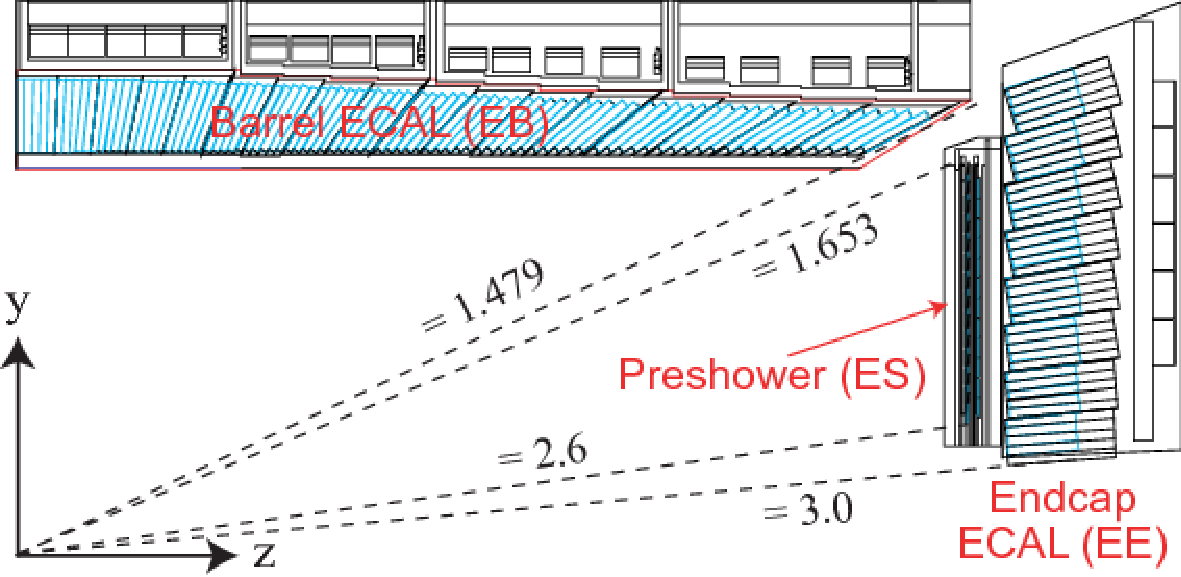
\includegraphics[width=0.45\textwidth]{fig_LHC_CMS/ECAL.pdf}
        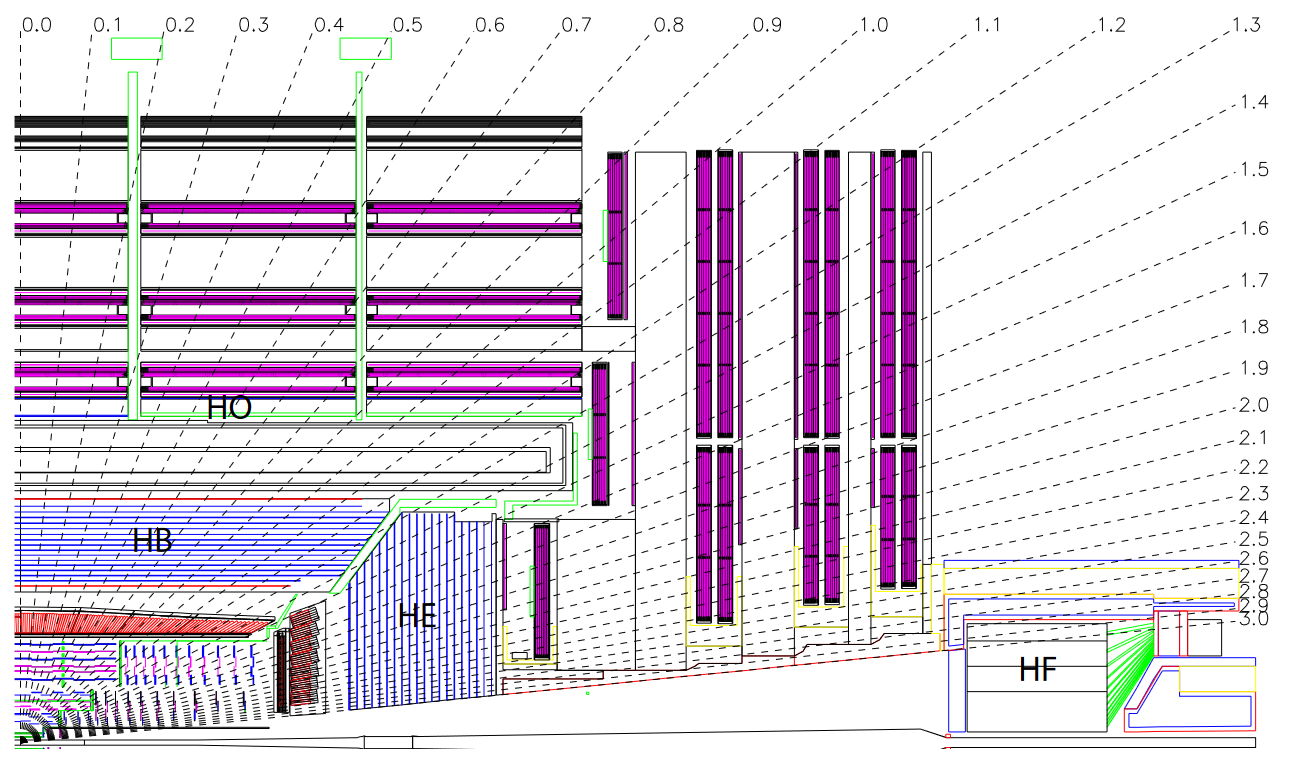
\includegraphics[width=0.40\textwidth]{fig_LHC_CMS/HCAL.png}
    \end{tabular}
    \caption{Schematic views of the ECAL (Left) ~\cite{Bayatian:922757} and HCAL (Right) ~\cite{Chatrchyan:1129810}.
            }
    \label{ECAL_HCAL}
  \end{center}
\end{figure}

\subsection{Hadronic Calorimeter}
Outside the ECAL is the hadronic calorimeter (HCAL), consisting of the HCAL Barrel (HB), which covers out to $\vert \eta \vert < 1.3$, the HCAL End-caps (HE), which cover $1.3 < \vert \eta \vert < 3$, and radiation-hard, quartz fiber hadron calorimeters that are placed in the forward region (HF) $3 < \vert \eta \vert < 5.2$ (see figure~\ref{ECAL_HCAL}).
The HCAL is designed to measure jet energy by forcing their strongly-interacting hadron constituents to shower in brass absorber layers that alternate with scintillating plastic layers, in which the showers deposit their energy by exciting nearby atoms which subsequently relax by emitting light collected by hybrid photodiodes.
The non-magnetic brass absorber layer is composed of 70\% \ce{Cu} and 30\% \ce{Zn} and has a nuclear interaction length of $\lambda_I = \SI{16.42}{\cm}$.
In the barrel region, the HB does not have sufficient total interaction length for hadron showers to completely exhaust their energy in the calorimeter, so an Outer HCAL (HO) of scintillating plastic layers, that uses the solenoid as an additional absorber layer, is placed outside the solenoid and covers out to $\vert \eta \vert < 1.3$.
The ECAL, which radially precedes the HCAL, contributes $1.1\lambda_I$.
At $\eta = 0$, the total interaction length of the absorber layers is $5.82\lambda_I$, and increases with $\eta$, so that at $\vert \eta \vert = 1.3$ it is $10.6\lambda_I$.

\subsection{Muon System}
Unlike most particles, muons are not stopped by any of the calorimeters, superconducting solenoid, or iron flux-return yoke. 
Four layers of chambers to detect muons are placed at the very outer layers of the experiment in the iron flux-return yoke. 
The muon system is designed with three different types of gaseous particle detectors: 
\begin{itemize}
\item drift tube (DT) chambers covering $\vert \eta \vert < 1.2$,
\item cathode strip chambers (CSC) covering $0.9 < \vert \eta \vert < 2.4$, and
\item resistive plate chambers (RPC) covering $\vert \eta \vert < 1.6$.
\end{itemize}
The layout for one quadrant of the muon system is shown in figure~\ref{Muon_System}.
The RPCs have inferior spatial resolution compared to the DTs and CSCs, but have excellent timing resolution and are primarily used for muon triggering.
The muon system is aligned with the inner tracker in order for the detectors to work together to identify muons and reconstruct their trajectories.
\begin{figure}[htb]
  \begin{center}
    \begin{tabular}{c}
        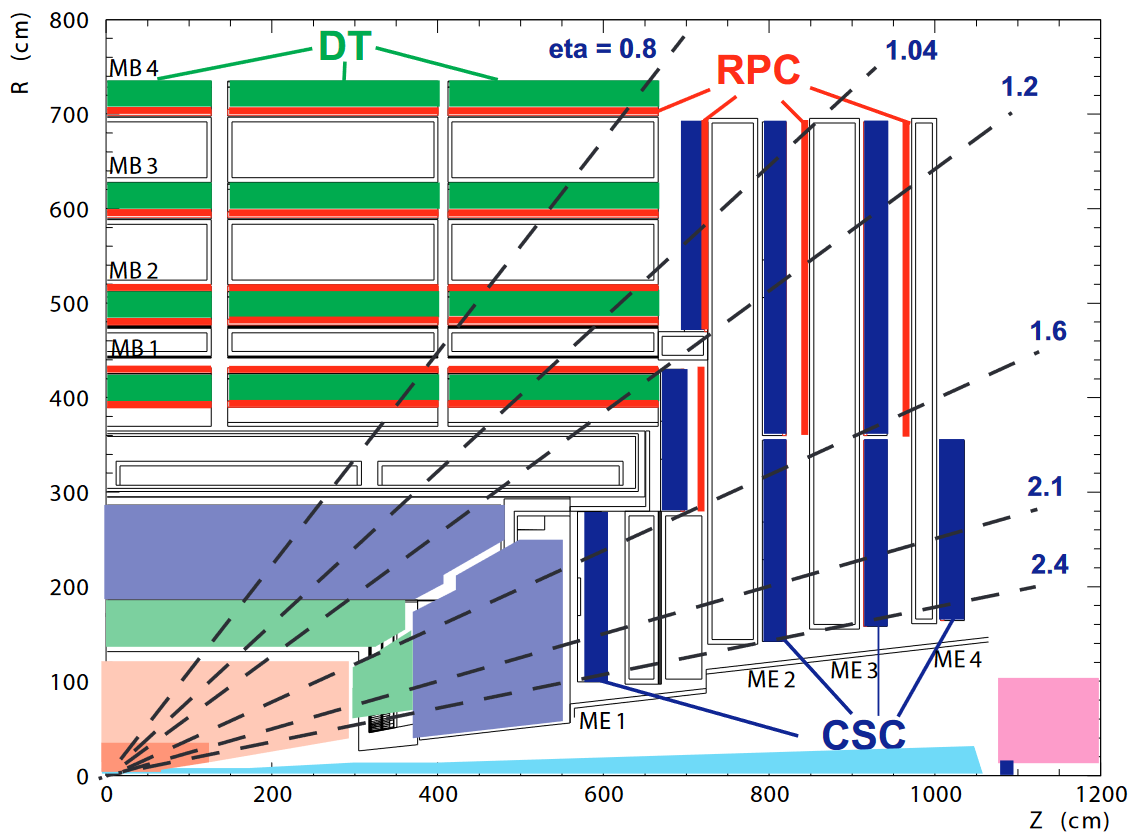
\includegraphics[width=0.65\textwidth]{fig_LHC_CMS/Muon_System.png}
    \end{tabular}
    \caption{Layout of one-quarter of the CMS muon system~\cite{Bayatian:922757}.
            }
    \label{Muon_System}
  \end{center}
\end{figure}

\subsection{Trigger and Data Acquisition System}
CMS wants to collect the most relevant data from bunch crossings with a $\SI{40}{\MHz}$ event rate.
Each bunch crossing generates \sim$\SI{1}{\M \byte}$ of data, but due to limited bandwidth, the detectors cannot readout and store \sim$\SI{40}{\T \byte \per \s}$, so a trigger system is necessary to reject the least interesting 99.9999\% of events in quasi-real time, and reduce the event rate to \sim$\SI{1}{\kilo \Hz}$ before storage.
This is not an unreasonable constraint, as the total cross-section of proton-proton interactions (elastic and inelastic) at \beamenergy is \sim$\SI{100}{\milli \b}$, while interesting processes such as top quark pair production and Higgs boson production have cross-sections on the orders of \sim$\SI{800}{\pico \b}$ and \sim$\SI{50}{\pico \b}$ respectively.
To accomplish this, CMS has a highly reliable and efficient trigger system, composed of detector electronics, a level-1 (L1) hardware trigger, a readout network, and a high-level software trigger (HLT).
The L1 trigger uses hardware processors and raw readouts from the calorimeters and muon systems to reduce the event rate to \sim$\SI{100}{\kHz}$ with a latency of $3.8 \; \mu s$.
The data acquisition then passes the complete readout of the event data to the HLT, which has a latency of $320 \; \mu s$ and performs fast reconstruction and event selection to filter events and reduce the rate of stored events to \sim$\SI{1}{\kilo \Hz}$.
The events that pass the HLT filter are saved for offline analysis to one or several HLT paths, which correspond to specific selection criteria, physics objects, or event signatures.




\ProvidesFile{chapters/ch-Top_Quark_Physics.tex}

\chapter{TOP QUARK PHYSICS AT THE LHC}
\label{Top_Quark_Physics_at_the_LHC}
The top quark was predicted in 1973 by Kobayashi and Maskawa, when the Cabibbo matrix was extended to the CKM matrix in order to accommodate the experimental discovery of CP-violation in precision measurements of kaon regeneration.
This extension necessarily required three quark generations, when at the time only the up, down, and strange quarks were known.
The charm quark was discovered in 1974 and the bottom quark in 1976.
After searching for two decades, the top quark was finally discovered in 1995 at Fermi National Acceleration Laboratory (FNAL), jointly by the CDF and D0 Tevatron Experiments.
It is the heaviest elementary particle ever discovered, with a measured mass $m_t = 172.69 \pm 0.30 \; \si{\GeV}$~\cite{bib:PDG}, the top quark has mass equivalent to a Tungsten isotope containing 184 nucleons; it is \sim$35$ times heavier than the next heaviest quark, the bottom quark~\ref{QuarkMasses}.
\begin{figure}[htb]
  \begin{center}
    \begin{tabular}{c}
        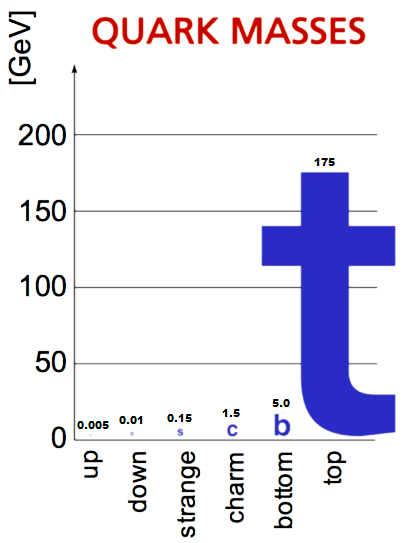
\includegraphics[width=0.325\textwidth]{fig_TopQuark/TopQuarkMass.png}
        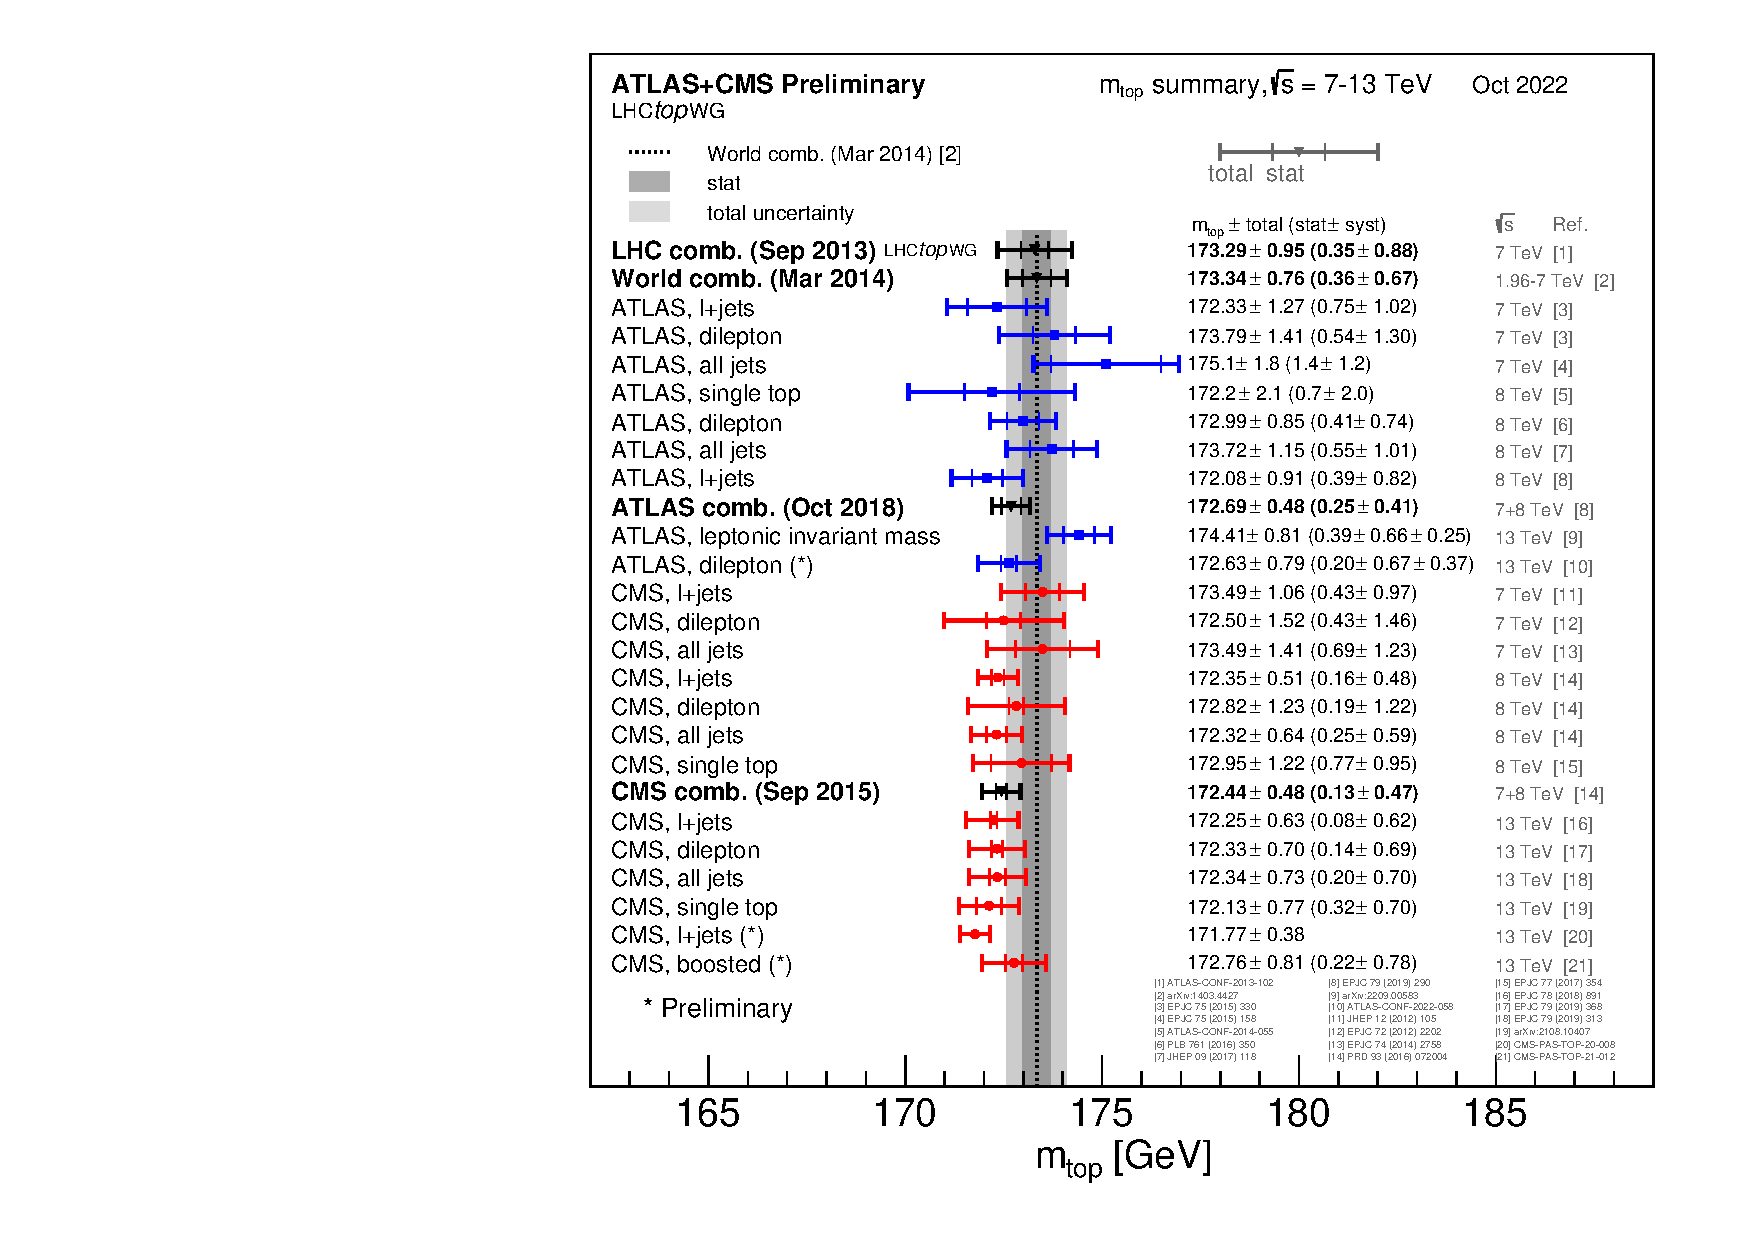
\includegraphics[width=0.45\textwidth]{fig_TopQuark/LHC_topmass_oct22.pdf}
    \end{tabular}
    \caption{The top quark is the heaviest elementary particle ever discovered and is \sim$35$ times heavier than the next heaviest quark (Left).
            Summary of the ATLAS and CMS direct measurements of top quark mass (Right)~\cite{LHCTopWGSummaryPlots}.
            }
    \label{QuarkMasses}
  \end{center}
\end{figure}
Due to its very large mass, the top quark has a very short life time, or equivalently, a large decay width.
The top quark full decay width is larger than the QCD hadronization scale and much larger than the spin decorrelation scale.
Thus, not only do the top quarks decay before hadronizing to form bound states, but also their properties, including spin information, are transferred to their decay products.
The spin information of top quarks is observable in the angular kinematic distributions of their decay products.
These properties makes top quarks unique in the quark sector, as top quark measurements are the only opportunity to study the properties of bare quarks, free of confinement effects.

\section{Top Quark Pair Production}
\label{Top_Quark_Pair_Production}
Because the large mass, production of top quarks have only been possible by Tevatron and LHC high-energy accelerator experiments.
At these colliders, the majority of top quarks are produced in \ttbar pairs by the strong interaction, but single $t$ production by the electroweak interaction is also possible.
For \ttbar production, three parton production processes are possible at hadron colliders: gluon-gluon ($gg$) fusion, quark/anti-quark ($q\bar{q}$) annihilation, and quark-gluon scattering.
While at the Tevatron quark$\slash$anti-quark annihilation was the dominant production mechanism, for \beamenergy proton-proton collisions at the LHC, the gluon density of the proton parton distribution function (PDF) is much higher than the quark density (see section~\ref{sec:Parton_Distribution_Functions}), and $gg$ fusion accounts for \sim$90 \%$ of \ttbar production.

The inclusive \ttbar production cross-section in proton-proton ($pp$) collisions is calculated by convoluting the proton PDFs with the partonic cross-sections, and summing over all parton constituents of the proton, i.e. gluons, valence quarks, and sea quarks.
For QCD \ttbar production, three channels of LO $gg$ fusion and one channel of LO $q\bar{q}$ annihilation parton production processes are possible.
LO Feynman diagrams for these processes are shown in figure~\ref{ttbar_production_LO_feynman_diagrams}.
\begin{figure}[htb]
  \begin{center}
    \begin{tabular}{cccc}
        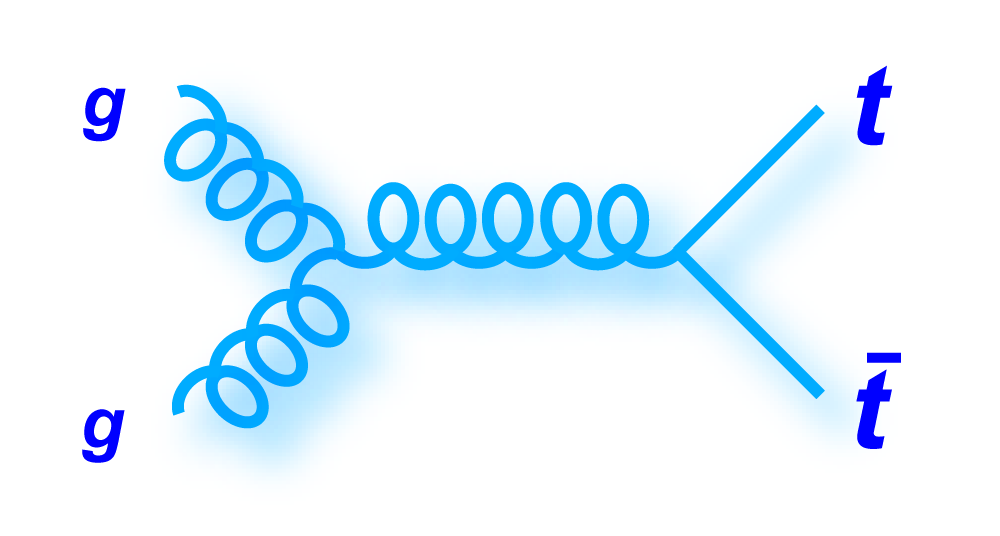
\includegraphics[width=0.225\textwidth]{fig_TopQuark/feynman_ttbar_LHC_gggtt.png}
        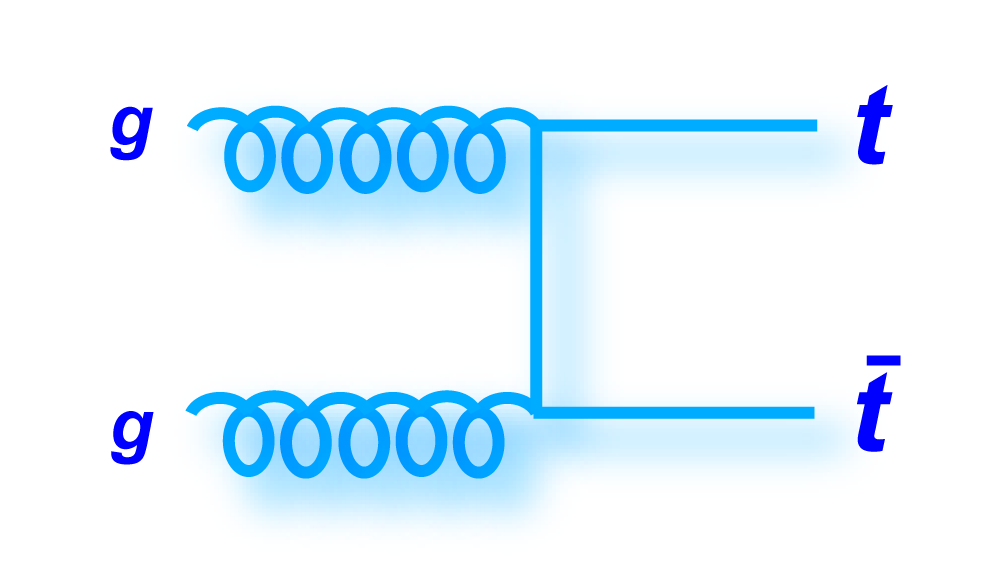
\includegraphics[width=0.225\textwidth]{fig_TopQuark/feynman_ttbar_LHC_ggttt.png}
        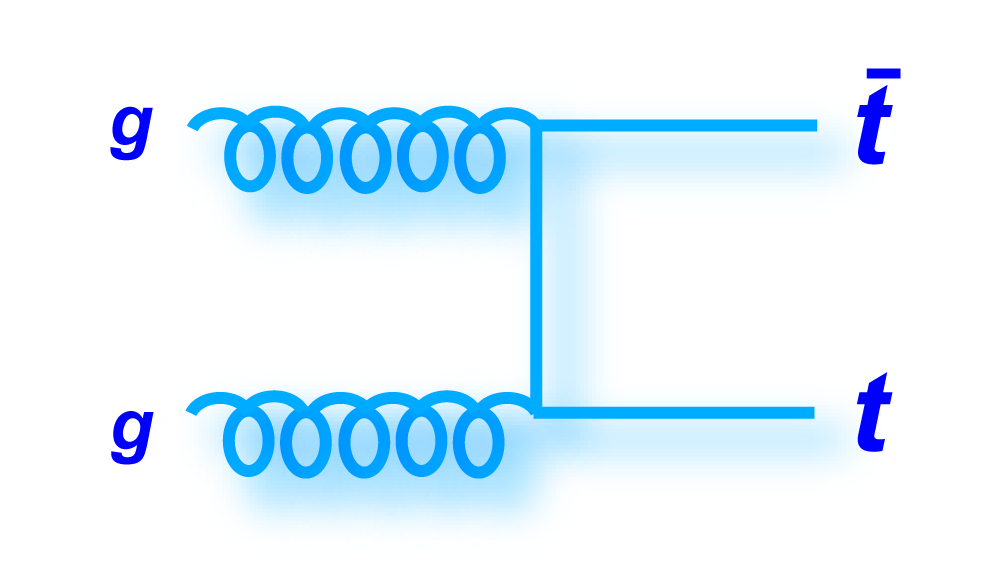
\includegraphics[width=0.225\textwidth]{fig_TopQuark/feynman_ttbar_LHC_ggttbart.png}
        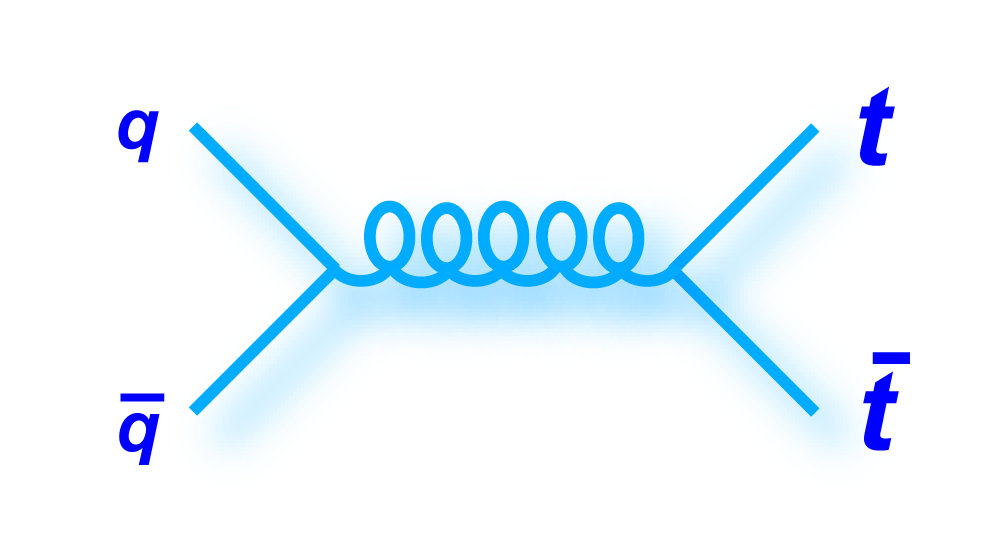
\includegraphics[width=0.225\textwidth]{fig_TopQuark/feynman_ttbar_LHC_qqgtt.png}
    \end{tabular}
    \caption{LO Feynman diagrams for QCD \ttbar production: three channels of $gg$ fusion and one channel of $q\bar{q}$ annihilation~\cite{d0_diagrams}.
            }
    \label{ttbar_production_LO_feynman_diagrams}
  \end{center}
\end{figure}
Quark-gluon scattering can also produce \ttbar pairs, but only at NLO and higher orders.
At NNLO with next-to-next-to-leading-logarithmic (NNLL) precision for \beamenergy, assuming $m_t = \SI{172.5}{\GeV}$, the inclusive \ttbar production cross-section is calculated to be $\sigma_{\ttbar} = 831.76 \substack{+19.77 \\ -29.20} \; (\text{Scale}) \; \pm 35.06 \; (\text{PDF} + \alpha_S) \; \si{\pico \b}$.
A summary of \ttbar cross-section measurements by LHC and Tevatron experiments as a function of the centre-of-mass energy, as well as a summary of \ttbar cross-section measurements by ATLAS and CMS at \beamenergy are shown in figure~\ref{ttbar_cross-section}.
\begin{figure}[htb]
  \begin{center}
    \begin{tabular}{cc}
        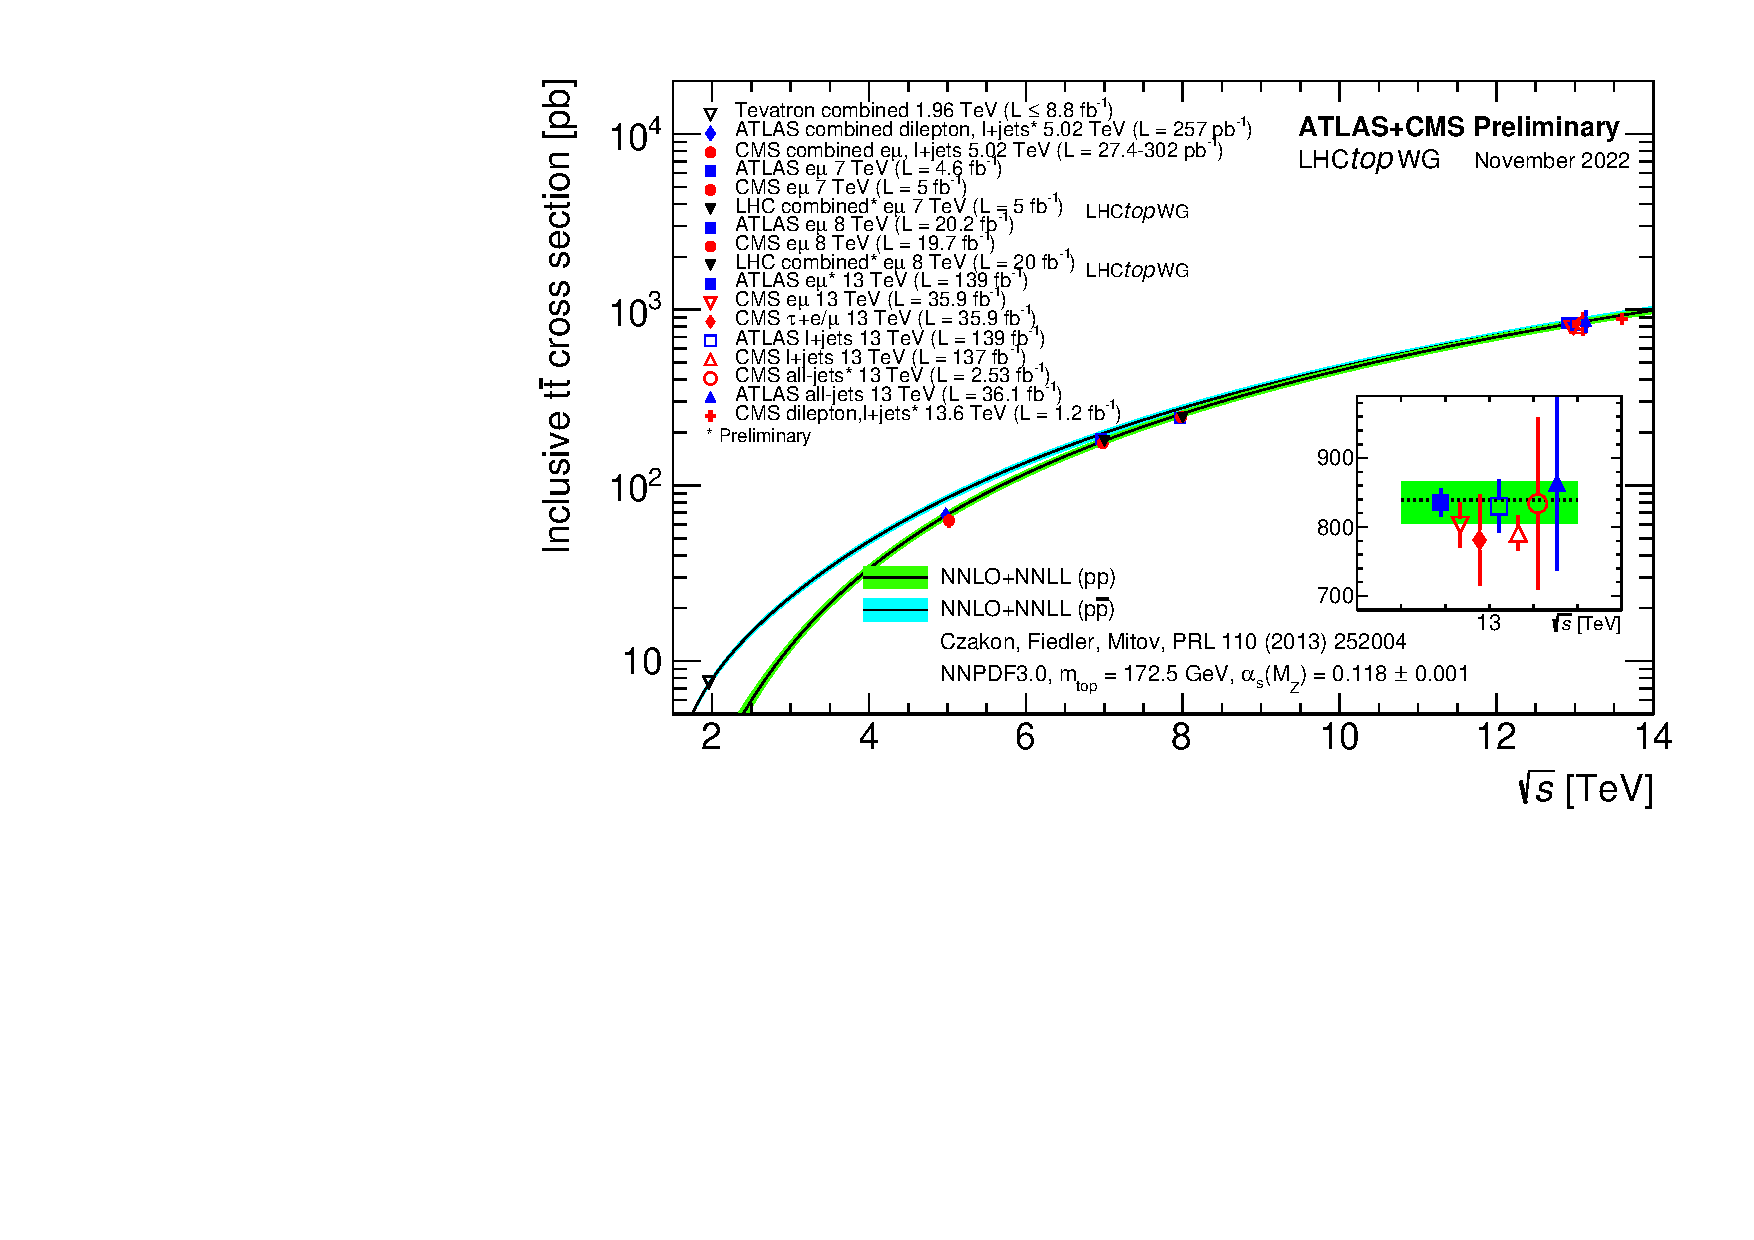
\includegraphics[width=0.50\textwidth]{fig_TopQuark/tt_curve_toplhcwg_nov22.pdf}
        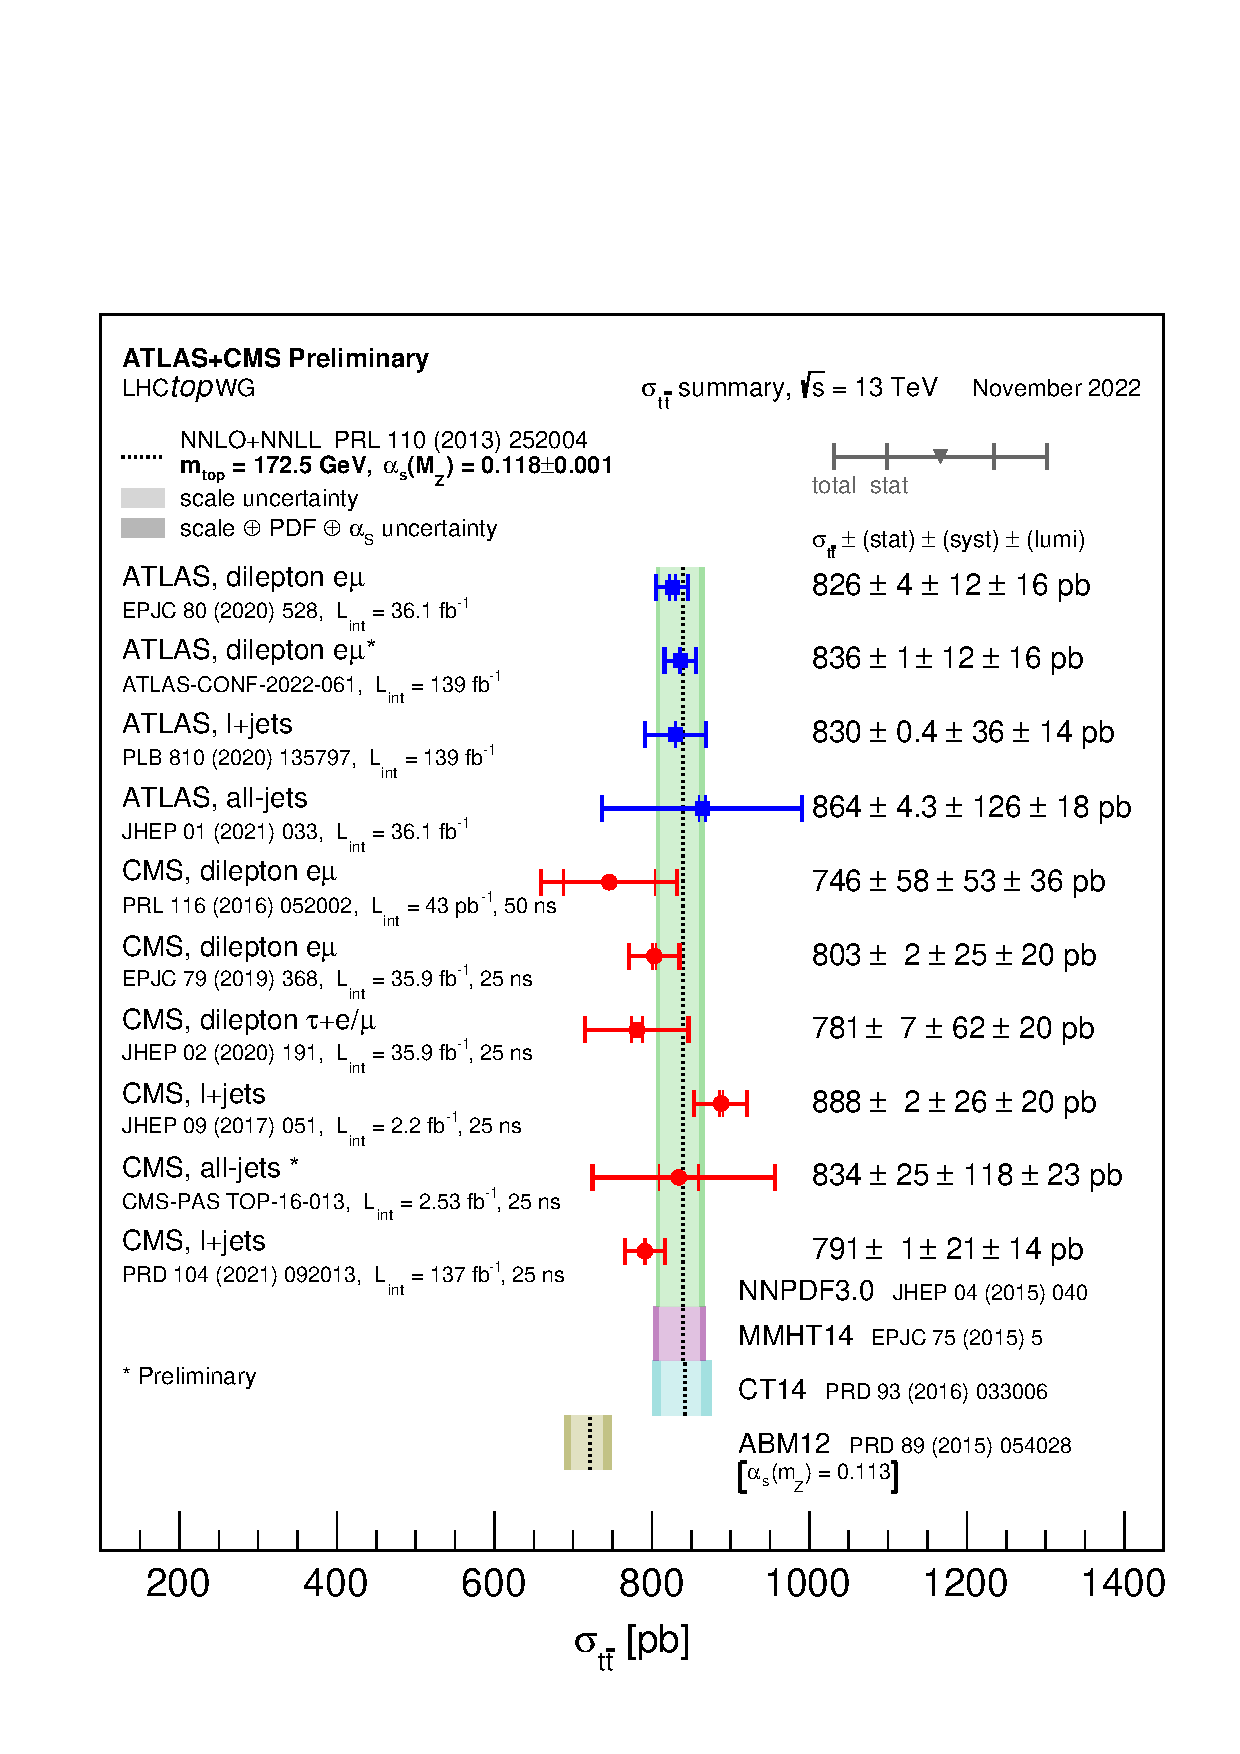
\includegraphics[width=0.30\textwidth]{fig_TopQuark/tt_xsec_13TeV_nov22.pdf}
    \end{tabular}
    \caption{Summary of LHC and Tevatron measurements of the top-pair production cross-section as a function of the centre-of-mass energy compared to the NNLO QCD calculation complemented with NNLL resummation (Left).
    Summary of measurements of the top-pair production cross-section at \beamenergy compared to the exact NNLO QCD calculation complemented with NNLL resummation (Right)~\cite{LHCTopWGSummaryPlots}.
            }
    \label{ttbar_cross-section}
  \end{center}
\end{figure}

\section{Decays of Top Quark Pairs}
\label{Decays_of_Top_Quark_Pairs}
The top quark decay width $\Gamma_t$ implies a lifetime of $\tau_t = \frac{1}{\Gamma_t}=\SI{4.6e-25}{\s}$ before decaying via the weak interaction into an on-shell $W$-boson and and down-type quark ($t \rightarrow W^+ q$).
The branching ratio of each mode can be calculated using elements of the CKM matrix $B_x = \frac{\vert V_{tx} \vert^2}{\vert V_{tb} \vert^2 + \vert V_{ts} \vert^2 + \vert V_{td} \vert^2}$, and while any of the down-type quarks are possible, because $\vert V_{tb} \vert = 0.999118 \; >> \; \vert V_{ts} \vert = 0.04110 \; \text{or} \; \vert V_{td} \vert = 0.00857$~\cite{bib:PDG}, $t \rightarrow W^+ b$ dominates with a branching ratio $ B_b \approx 99.8\%$.

The $W$-boson can decay hadronically $W^+ \rightarrow q \bar{q^\prime}$, where $q$ is an up-type quark ($u$ or $c$) and $\bar{q^\prime}$ is an anti-down-type quark ($\bar{d}$, $\bar{s}$, or $\bar{b}$), or leptonically $W^+ \rightarrow \bar{\ell} \nu_\ell$, where $\bar{\ell}$ is an anti-lepton ($\bar{e}$, $\bar{\mu}$, or $\bar{\tau}$) and $\nu_\ell$ is a neutrino of the same lepton flavor~\ref{t_decay}.
\begin{figure}[htb]
  \begin{center}
    \begin{tabular}{cc}
        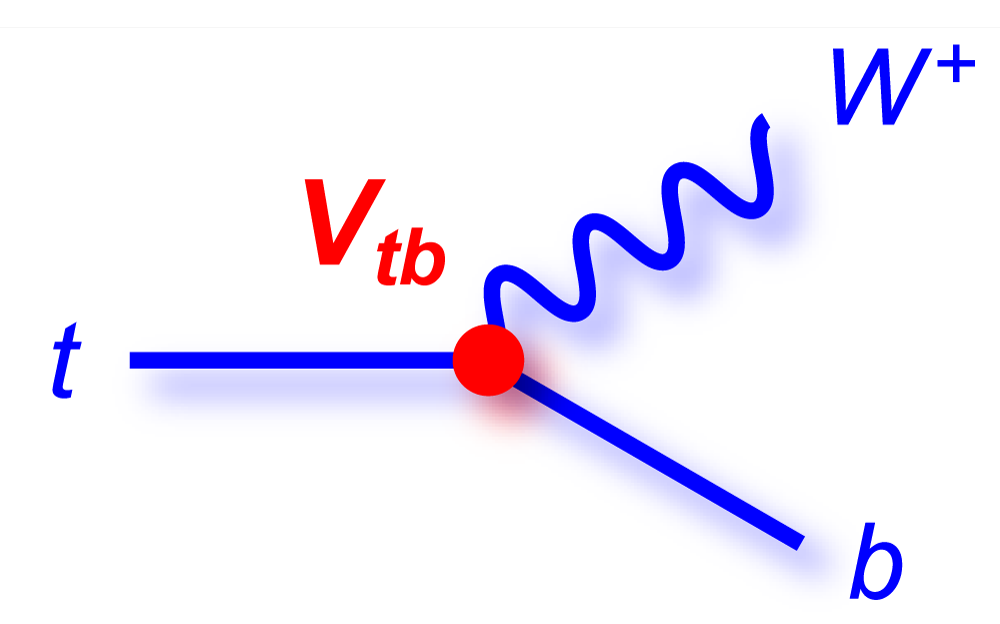
\includegraphics[width=0.30\textwidth]{fig_TopQuark/feynman_t_decay_Vtb_blue.png}
        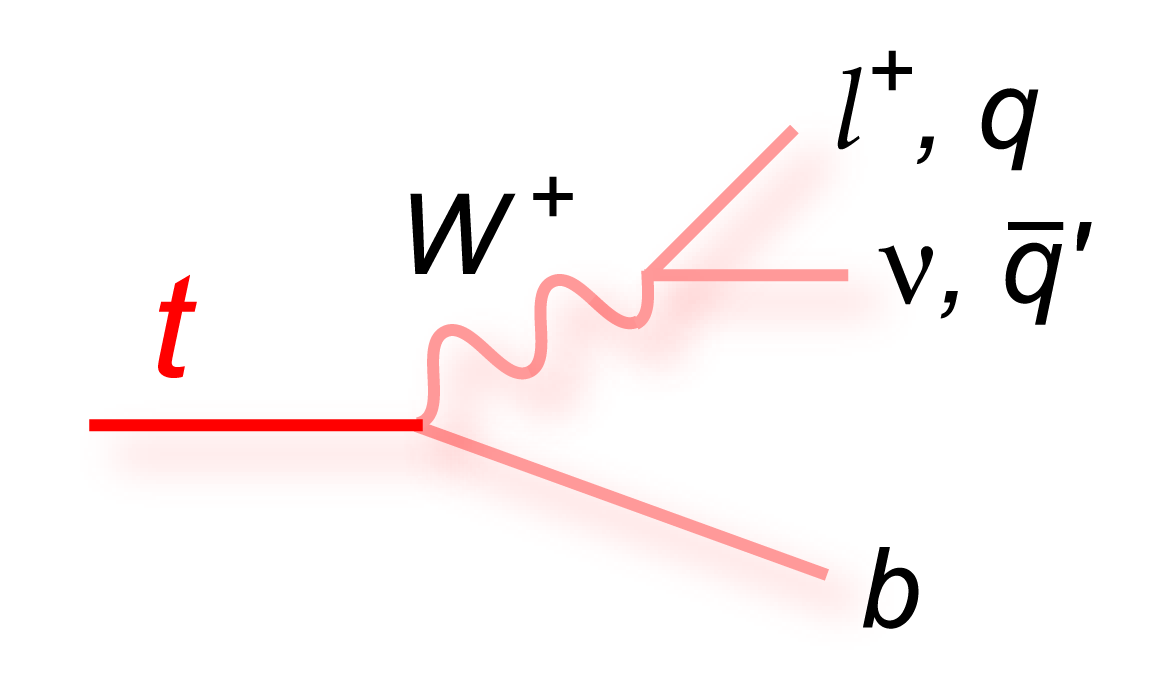
\includegraphics[width=0.30\textwidth]{fig_TopQuark/feynman_t_decay_ljetsqq_pink.png}
    \end{tabular}
    \caption{The branching modes of $t \rightarrow W^+ q$ depend on the values of CKM matrix elements (Left).
             The $W$-boson can decay hadronically or leptonically (Right)~\cite{d0_diagrams}.
    }
    \label{t_decay}
  \end{center}
\end{figure}
Ignoring phase space considerations, the relative branching fractions of the hadronic and leptonic decay modes are given by the ratio of flavor combinations and color combinations, together with the corresponding squared CKM matrix elements:
\begin{linenomath*}
{\small
\begin{align}
\frac{\text { hadronic }}{\text { leptonic }}=\frac{ \{ u\bar{d}:{\vert V_{ud} \vert}^2, u\bar{s}:{\vert V_{us} \vert}^2, u\bar{b}:{\vert V_{ub} \vert}^2, c\bar{d}:{\vert V_{cd} \vert}^2, c\bar{s}:{\vert V_{cs} \vert}^2, c\bar{b}:{\vert V_{cb} \vert}^2 \} \times \{ R, B, G\} }{ \{ e \bar{\nu_e }, \mu \bar{\nu_\mu}, \tau \bar{\nu_\tau} \}} = \frac{6}{3}
\end{align}
}%
\end{linenomath*}
where decays with top quarks are forbidden due to energy conservation, and due to the unitary of the CKM matrix ${\vert V_{ud} \vert}^2 + {\vert V_{us} \vert}^2 + {\vert V_{ub} \vert}^2 = {\vert V_{cd} \vert}^2 + {\vert V_{cs} \vert}^2 + {\vert V_{cb} \vert}^2 = 1$.
Including phase space considerations, the hadronic $W$-boson decay mode occurs \sim$67.4 \%$ of the time, and the lepton mode occurs the other \sim$32.6 \%$~\cite{bib:PDG}.

For a \ttbar pair, depending on the $W$-boson decays of the $t$ and $\bar{t}$, there are three decay modes: 
\begin{itemize}
    \item {\bf Fully Hadronic:} $t\bar{t} \rightarrow W^+ b \; W^- \bar{b} \rightarrow q \bar{q^\prime} b \; \bar{q^{\prime\prime}}  q^{\prime\prime\prime} \bar{b}$, also referred to as "all jets"
    \item {\bf Semi-Leptonic:} $t\bar{t} \rightarrow W^+ b \; W^- \bar{b} \rightarrow  q \bar{q^\prime} b \; \ell \bar{\nu_{\ell}} \bar{b} $ or $t\bar{t} \rightarrow W^+ b \; W^- \bar{b} \rightarrow  \bar{\ell} \nu_\ell b \; \bar{q^{\prime\prime}}  q^{\prime\prime\prime} \bar{b}$, also referred to as "lepton + jets"
    \item {\bf Dileptonic:} $t\bar{t} \rightarrow W^+ b \; W^- \bar{b} \rightarrow \bar{\ell} \nu_\ell b \; \ell^{\prime} \bar{\nu_{\ell^{\prime}}} \bar{b}$
\end{itemize}
Examples of LO Feynman diagrams for the \ttbar decay modes are shown in figure~\ref{Top_Pair_Decay_FeynmanDiagrams}.
\begin{figure}[htb]
  \begin{center}
    \begin{tabular}{c}
        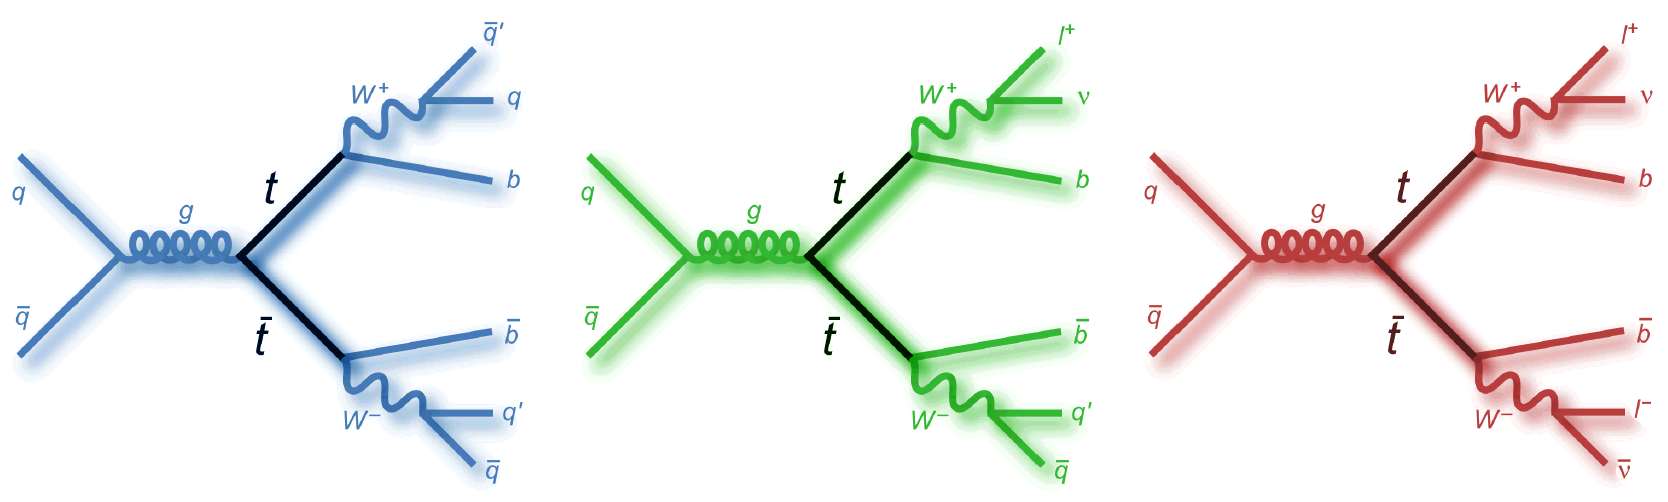
\includegraphics[width=0.90\textwidth]{fig_TopQuark/ttbar_decay_feynman_diagrams.png}
    \end{tabular}
    \caption{Examples of LO Feynman diagrams for the \ttbar decay modes: Fully Hadronic (Left), Semi-Leptonic (Middle), and Dileptonic (Right)~\cite{d0_diagrams}
            }
    \label{Top_Pair_Decay_FeynmanDiagrams}
  \end{center}
\end{figure}
Because hadronic $W$-boson decay modes are more common than leptonic ones, for \ttbar decays the dileptonic mode occurs least often \sim$10.7 \%$~\cite{bib:PDG}.
A schematic classifying \ttbar decay modes, together with a chart showing the relative branching fractions, is shown in figure~\ref{Top_Pair_Decay_Channels}.
\begin{figure}[htb]
  \begin{center}
    \begin{tabular}{cc}
        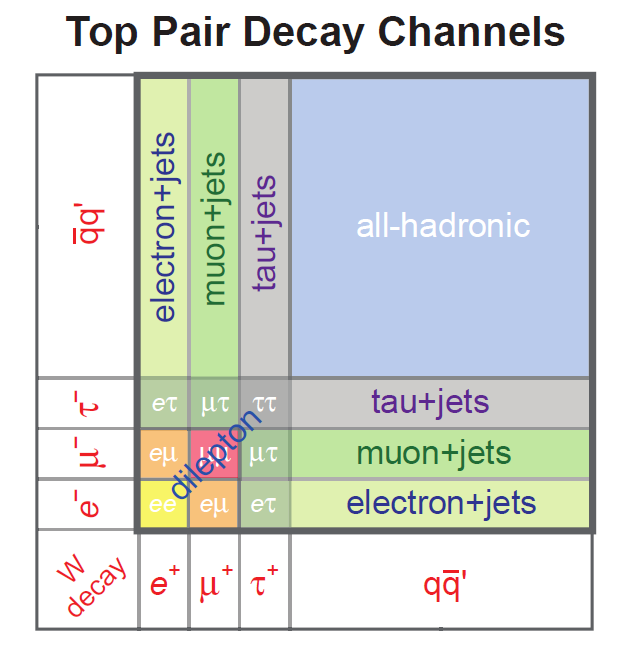
\includegraphics[width=0.40\textwidth]{fig_TopQuark/Top_Pair_Decay_Channels.png}
        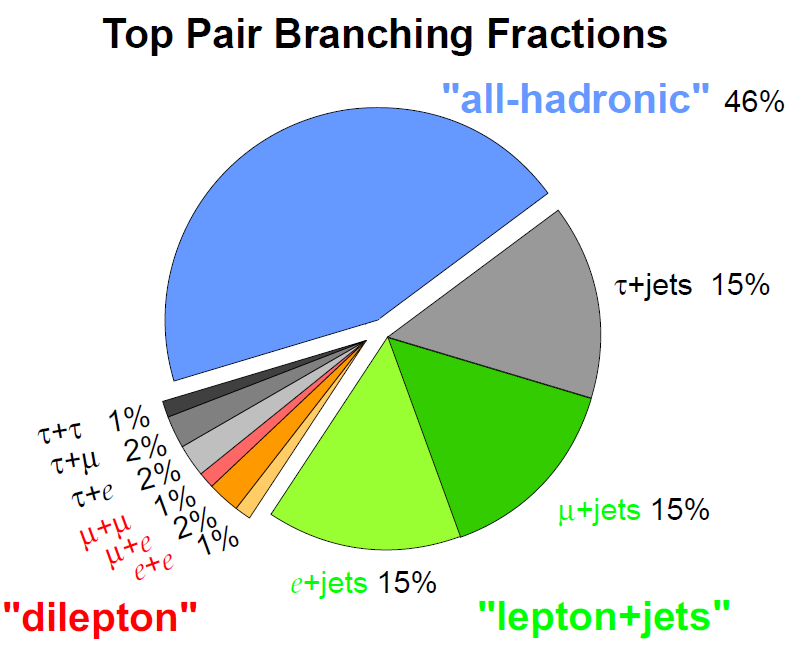
\includegraphics[width=0.45\textwidth]{fig_TopQuark/Top_Pair_Branching_Fractions.png}
    \end{tabular}
    \caption{A schematic classifying \ttbar decay modes (Left), and chart showing the relative branching fractions (Right)~\cite{d0_diagrams}
            }
    \label{Top_Pair_Decay_Channels}
  \end{center}
\end{figure}

Furthermore, $\tau$ can decay either hadronically or leptonically via a virtual $W$-boson.
For lepton decays of $\tau \rightarrow \ell \bar{\nu_\ell} \nu_\tau$, the $\tau$ decays into a lepton, an anti-neutrino of the same lepton flavor, and a $\tau$ flavor neutrino.
The lepton branching fractions of $\tau$ decays are \sim$17.82 \%$ for $\ell = e$ and \sim$17.39 \%$ for $\ell = \mu$~\cite{bib:PDG}.
Including $\tau$ decays, the \ttbar dileptonic final state branching fraction is \sim$6.42 \% = $ \sim$4.55 \% (\text{Prompt}) + $ \sim$1.87 \% (\text{Via Tau})$.
The \ttbar dileptonic final state is further categorized into three channels: \ee, \emu, and \mumu, with the combination of the three channels denoted $\ell \bar{\ell}$.

\section{Top Quark Spin in \ensuremath{\mathrm{t\bar{t}}} Production and Top Decay}
\label{Top_Quark_Spin_in_ttbar_Production_and_Top_Decay}
In general, hadronization of quarks dilutes their spin information.
Moreover, the spins of quarks can be depolarized by processes such as gluon radiation, causing spin decorrelation.
For the top quark however, it has already been mentioned that the full decay width $\Gamma_t = 1.42 \substack{+0.19 \\ -0.15} \; \si{\GeV}$~\cite{bib:PDG} is larger than the QCD hadronization scale ($\lambda_{QCD} \approx \SI{0.38}{\GeV}$~\cite{Groote_1998}) and much larger than the spin decorrelation scale ($\lambda_{QCD}^2/m_t \sim \SI{0.08}{\MeV}$~\cite{Stelzer_1996}).
Thus, not only does a top quark decay before hadronizing to form bound states, but also its spin properties are transferred, without dilution, to its decay products and that information is observable in their angular kinematic distributions.
These properties makes top quarks unique in the quark sector, as top quark measurements are the only opportunity to study the spin properties of free quarks.

For the spin quantization axes, we consider the top quark helicity basis ($\hat{k}, \hat{n}, \hat{r}$) in the zero momentum frame (ZMF) of the \ttbar system.
In this reference frame, the helicity axis $\hat{k}$, is defined as the direction of the top quark.
The axis $\hat{n}$ is transverse to the production plane made by $\hat{k}$ direction of the incoming parton $\hat{p}$, i.e. the direction of the proton beam $\hat{z}$, and the axis $\hat{r}$ is orthogonal to the other two axes, forming a right-handed coordinate system:
\begin{linenomath*}
\begin{align}
\begin{array}{c}
\hat{n}=\frac{\operatorname{sign}(\cos \Theta)}{\sin \Theta}(\hat{p} \times \hat{k}) \\
\hat{r}=\frac{\operatorname{sign}(\cos \Theta)}{\sin \Theta}(\hat{p} - \hat{k}\cos \Theta)
\end{array}
\label{helcity_basis}
\end{align}
\end{linenomath*}
where $\Theta$ is the top quark scattering angle and $\operatorname{sign}(\cos \Theta)$ helps defines a “forward” direction for each event, the importance of which will be made explicit later, so that $\hat{n}$ and $\hat{r}$ flip signs as $\Theta$ crosses $\frac{\pi}{2}$.
The helicity basis spin quantization axes are shown in figure~\ref{helicity_basis}.
\begin{figure}[htb]
  \begin{center}
    \begin{tabular}{c}
        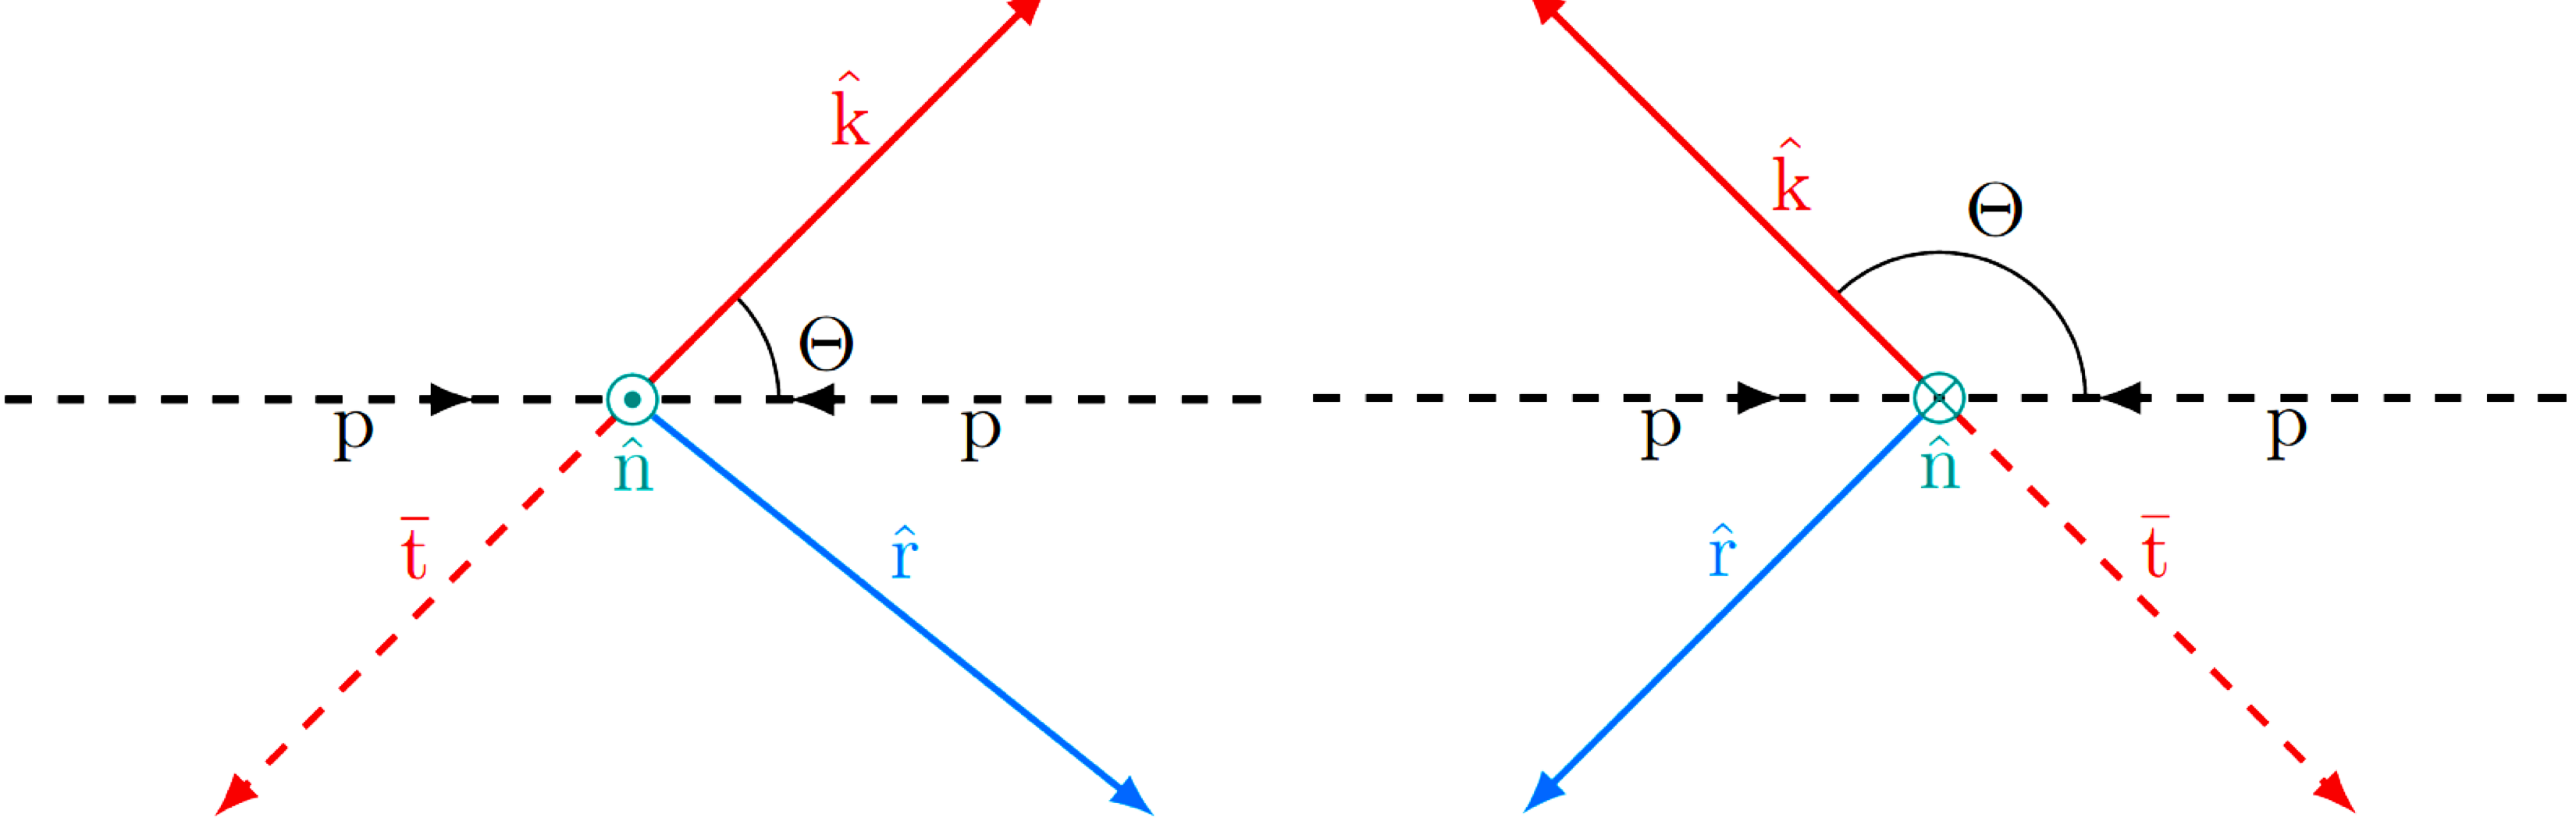
\includegraphics[width=0.9\textwidth]{fig_TopQuark/helicity_basis.png}
    \end{tabular}
    \caption{The helicity basis spin quantization axes in the \ttbar ZMF;
            $\hat{n}$ and $\hat{r}$ flip signs as $\Theta$ crosses $\frac{\pi}{2}$.
            }
    \label{helicity_basis}
  \end{center}
\end{figure}

At LO, the kinematic and spin properties of a \ttbar pair can be completely described in the \ttbar ZMF by the invariant mass $m_{\ttbar}$ and the top scattering angle $\Theta$.
Helicity is defined as spin direction projected onto the linear momentum direction, and for massive particles, helicity is reference frame dependent.
In the helicity basis of the \ttbar ZMF, squared matrix elements (see section~\ref{sec:Matrix_Element_Calculation_and_Production_Cross-section}) for the $q\bar{q}$ annihilation LO Feynman diagram in figure~\ref{ttbar_production_LO_feynman_diagrams} separated into like-helicity ($L L, R R$) and unlike-helicity ($L R, R L$) \ttbar pairs are~\cite{PhysRevD.53.4886}:
\begin{linenomath*}
\begin{align}
\begin{array}{c}
\sum_{L L, R R}\vert\mathcal{M}(q \bar{q} \rightarrow t \bar{t})\vert^2=8 (4 \pi \alpha_S)^2 \left(1-\beta^2\right) \sin ^2 \Theta \\
\sum_{L R, R L}\vert\mathcal{M}(q \bar{q} \rightarrow t \bar{t})\vert^2=8 (4 \pi \alpha_S)^2 \left(1+\cos ^2 \Theta\right)
\end{array}
\label{qq_matrix_elements}
\end{align}
\end{linenomath*}
where $\beta=\sqrt{1-4 m_t^2 / m_{\ttbar}^2}$ is the speed of the top quark (as a fraction of $c$) in the \ttbar ZMF and is completely determined by $m_{\ttbar}$.
In the helicity basis of the \ttbar ZMF, squared matrix elements for the $gg$ fusion LO Feynman diagram in figure~\ref{ttbar_production_LO_feynman_diagrams} separated into like-helicity ($L L, R R$) and unlike-helicity ($L R, R L$) \ttbar pairs are~\cite{PhysRevD.53.4886}:
\begin{linenomath*}
\begin{align}
\begin{array}{c}
\sum_{L L, R R}\vert\mathcal{M}(g g \rightarrow t \bar{t})\vert^2=\frac{16}{3} (4 \pi \alpha_S)^2 (\frac{7+9 \beta^2 \cos ^2 \Theta}{\left(1-\beta^2 \cos ^2 \Theta\right)^2}) \left(1-\beta^2\right)\left(1+\beta^2+\beta^2 \sin ^4 \Theta\right) \\
\sum_{L R, R L}\vert\mathcal{M}(g g \rightarrow t \bar{t})\vert^2=\frac{16}{3} (4 \pi \alpha_S)^2 (\frac{7+9 \beta^2 \cos ^2 \Theta}{\left(1-\beta^2 \cos ^2 \Theta\right)^2}) \beta^2 \sin ^2 \Theta\left(1+\cos ^2 \Theta\right).
\end{array}
\label{gg_matrix_elements}
\end{align}
\end{linenomath*}
These expressions include summation over the spins of the incoming partons, as well as summation over the colors of both the incoming and outgoing states, but factors averaging over the spins and colors have not been included.

Equations~\ref{qq_matrix_elements} indicate that in the high energy limit ($\beta \rightarrow 1$), the production of like-helicity \ttbar pairs by $q\bar{q}$ annihilation is suppressed.
Equations~\ref{gg_matrix_elements} indicate that in the high energy limit ($\beta \rightarrow 1$), the production of like-helicity \ttbar pairs by $gg$ fusion is also suppressed, but additionally at low energies $\beta << 1$, production of unlike-helicity \ttbar pairs is suppressed relative to the production of like-helicity pairs by a factor ($\beta^2$).
The breakdown of the total \ttbar cross section into like-helicity and unlike-helicity pairs as a function of $m_{\ttbar}$ using the helicity basis for the $\sqrt{s}=\SI{14}{\TeV}$ LHC is shown in figure~\ref{LHC_ttbar_helicity_differential}.
Near threshold, the dominant spin states of the \ttbar system are ${}^{1}S_{0}$ for like-helicity \ttbar pairs from $gg$ fusion and ${}^{3}S_1$ for unlike-helicity \ttbar pairs from $q\bar{q}$ annihilation:
\begin{linenomath*}
\begin{align}
\begin{array}{ccc}
& & \vert \uparrow \uparrow \rangle \\
{}^{1}S_{0} :& \frac{1}{\sqrt{2}}[\vert \uparrow \downarrow \rangle - \vert \downarrow \uparrow \rangle] \quad \quad \quad \quad {}^{3}S_1 :& \frac{1}{\sqrt{2}}[\vert \uparrow \downarrow \rangle + \vert \downarrow \uparrow \rangle] \\
& &\vert \downarrow \downarrow \rangle \\
\end{array}
\end{align}
\end{linenomath*}
where the first (second) arrow of $\vert \uparrow \downarrow \rangle$ refer to the spin state of the top quark (anti-quark) along spin quantization axis $\hat{i}$ ($\hat{j}$).
The different parton production processes and helicity combinations manifest themselves in the \ttbar final state particle angular kinematic distributions.
\begin{figure}[htb]
  \begin{center}
    \begin{tabular}{c}
        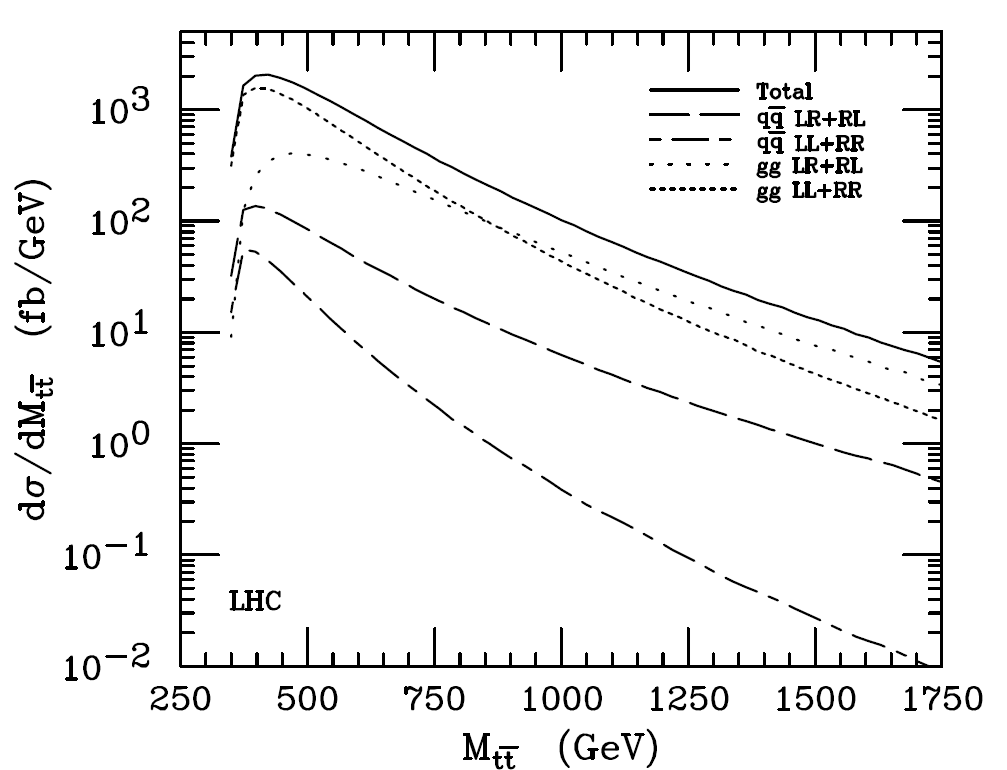
\includegraphics[width=0.7\textwidth]{fig_TopQuark/LHC_ttbar_helicity_differential.png}
    \end{tabular}
    \caption{Differential cross section for \ttbar production as a function of $m_{\ttbar}$, for the $\sqrt{s}=\SI{14}{\TeV}$ LHC, decomposed into $L L + R R$ and $L R + R L$ helicities in the zero momentum frame of the \ttbar pair for both $q\bar{q}$ and $gg$ components using the helicity basis~\cite{PhysRevD.53.4886}.
            }
    \label{LHC_ttbar_helicity_differential}
  \end{center}
\end{figure}

The differential decay rate of top quark daughter or granddaughter particle $x$, for an ensemble of polarized top quarks at rest with polarization $0 \leq \vect{P} \leq 1$, can be parameterized~\cite{BRANDENBURG2002235} as:
\begin{linenomath*}
\begin{align}
\frac{1}{\Gamma} \frac{d \Gamma}{d\left(\cos \theta_x\right)}=\frac{1}{2}[1+ \vert \vect{P} \vert \kappa_x \cos \theta_x]
\end{align}
\end{linenomath*}
where $\theta_x$ is the angle between $\vect{P}$ and the momentum direction of $x$ in the top quark ZMF and $\kappa_x$ is the top spin analyzing power of particle $x$, denoting what fraction of the top polarization information gets transferred from the top to its daughter or granddaughter particle $x$.
The top spin analyzing power at NLO is shown for the various daughter and granddaughter particles table~\ref{spin_analyzing_power_NLO}.
\begin{table}[htb]
\begin{center}
\begin{tabular}{lr}
\multicolumn{2}{c}{ Top Spin Analyzing Power at NLO } \\
\hline$\kappa_b$ & $-0.39$ \\
$\kappa_{W^{+}}$ & $0.39$ \\
$\boldsymbol{\kappa}_{\ell}$ & $\mathbf{0.998}$ \\
$\kappa_{\bar{d}, \bar{s}}$ & $0.93$ \\
$\kappa_{u, c}$ & $-0.31$
\end{tabular}
\caption{The top spin analyzing power at NLO for the various daughter and granddaughter decay particles of the top quark~\cite{BRANDENBURG2002235}.
         }
\label{spin_analyzing_power_NLO}
\end{center}
\end{table}
For charged lepton granddaughters of top quarks, the top spin analyzing power ($\kappa_\ell$) is close to unity, and when combined with the experimental advantages that charged leptons can be triggered on efficiently and reconstructed precisely, it is concluded that the leptonic decay mode is the optimal proxy for studies of top quark spin properties.

\section{Top Quark Polarizations and \ensuremath{\mathrm{t\bar{t}}} Spin Correlations}
\label{Top_Quark_Polarizations_and_ttbar_Spin_Correlations}
Top quarks and anti-quarks, produced in \ttbar pairs at hadron colliders via the strong interaction, are not polarized at LO due to the parity conserving nature of QCD (longitudinal polarization) and approximate T-invariance of QCD (transverse polarization).
However, as was shown in the previous section, the spins of top quarks produced in \ttbar pairs are strongly correlated with spins of anti-top quarks, with dependence on $m_{\ttbar}$, $\Theta$, and choice of spin quantization axes. 
The squared matrix element for the \ttbar production and decay can be written as~\cite{Bernreuther}:
\begin{linenomath*}
\begin{align}
\begin{array}{c}
\vert\mathcal{M}(gg/q\bar{q} \to \ttbar \to (\bar{\ell} \nu_\ell b)(\ell^\prime \bar{\nu_{\ell^\prime}} \bar{b}) )\vert^2 \sim Tr[\rho R \bar{\rho}]
\end{array}
\label{ttbar_squared_matrix_element}
\end{align}
\end{linenomath*}
where $R$ is the spin density matrix related to on-shell \ttbar production and $\rho$ is the decay density matrix.
The production spin density matrix $R$ can be decomposed in the spin spaces of $t$ and $\bar{t}$ using a basis of Pauli matrices~\cite{Bernreuther}:
\begin{linenomath*}
\begin{align}
R^I \propto \tilde{A} \mathbbm{1} \otimes  \mathbbm{1} + \tilde{B}_i^+ \sigma^i \otimes \mathbbm{1} + \tilde{B}_j^- \mathbbm{1} \otimes \sigma^j + \tilde{C}_{ij} \sigma^i \otimes \sigma^j
\label{spin_density_matrix_decomposition}
\end{align}
\end{linenomath*}
where intial state $I = gg / q\bar{q}$ at fixed energy and top direction, $\tilde{A}$ determines the differential cross section for \ttbar production, $\mathbbm{1}$ is the $2\times2$ identity matrix, $\sigma^{i(j)}$ are the Pauli matrices, $\tilde{B}^\pm$ are 3-vectors that characterize the top quark ($+$) and anti-quark ($-$) polarizations along each of the spin quantization axes, and $\tilde{C}$ is a $3\times3$ matrix that characterizes the correlations between the top quark and anti-quark spins along each pair of spin quantization axes.
$\tilde{B}_i^\pm$ and $ \tilde{C}_{ij} $ can be further decomposed using the \ttbar ZMF helicity basis $\{\hat{k},\hat{n},\hat{r}\}$~\cite{Bernreuther}:
\begin{linenomath*}
\begin{align}
\begin{array}{l}
\tilde{B}_i^\pm =  b_k^\pm \hat{k_i} + b_n^\pm \hat{n_i} + b_r^\pm \hat{r_i} \\
\tilde{C}_{ij}  =  c_{kk} \hat{k_i}\hat{k_j} + c_{nn} \hat{n_i}\hat{n_j} + c_{rr} \hat{r_i}\hat{r_j} \\ 
\;\;\;\;\; + \; c_{rk} (\hat{r_i}\hat{k_j} + \hat{k_i}\hat{r_j}) +  c_{kn} (\hat{k_i}\hat{n_j} + \hat{n_i}\hat{k_j})  +  c_{nr} (\hat{n_i}\hat{r_j} + \hat{r_i}\hat{n_j}) \\
\;\;\;\;\; + \; c_{n} (\hat{r_i}\hat{k_j} - \hat{k_i}\hat{r_j}) +  c_{r} (\hat{k_i}\hat{n_j} - \hat{n_i}\hat{k_j})  +  c_{k} (\hat{n_i}\hat{r_j} - \hat{r_i}\hat{n_j})
\end{array}
\label{spin_density_matrix_decomposition_expansion}
\end{align}
\end{linenomath*}
where the coefficients $b^\pm$ and $c$ are functions of $m_{\ttbar}$ and $\cos \Theta$.
The helicity basis is chosen is because of its stability with regard to reconstruction errors and the spin correlations are strong using this basis.
By construction, the coefficient functions $b^\pm$ and $c$ have definite properties with respect to discrete symmetries $P$, $CP$, $T_N$ (naive time-reversal symmetry at tree-level), and identical particle exchange ($Bose$), and as a result, these coefficients can help distinguish NP effects with SMEFT~\cite{Bernreuther}.
The $P$, $CP$, and $T$ invariance of QCD forces many of these coefficients to be small or zero before considering electroweak and higher-order QCD loop corrections.
The Bose symmetry of $I = gg$ implies $R^{gg}(\hat{k},\hat{p}) = R^{gg}(-\hat{k},\hat{p})$; hence the importance of $\operatorname{sign}(\cos \Theta)$ in the definition of $\{\hat{k},\hat{n},\hat{r}\}$(see equation~\ref{helcity_basis}), to allow non-zero coefficients when the parton production process is $gg$ fusion.
A summary of transformation properties of the coefficient functions with respect to $P$, $CP$, $T_N$, and $Bose$ ($I = gg$ only) symmetries~\cite{Bernreuther} is shown in table~\ref{coefficient_function_symmetries}, 
\begin{table}[htb]
\begin{center}
\begin{math}
\begin{array}{|c|c|c|c|c|c|}
\hline
& \mathrm{CP} & \mathrm{P} & \mathrm{T}_{\mathrm{N}} & \mathrm{CPT}_{\mathrm{N}} & \text { Bose } \\
\hline 
A^I & A^I & A^I & A^I & A^I & A^{g g} \\
b_r^{I \pm} & b_r^{I \mp} & -b_r^{I \pm} & b_r^{I \pm} & b_r^{I \mp} & b_r^{g g \pm} \\
b_k^{I \pm} & b_k^{I \mp} & -b_k^{I \pm} & b_k^{I \pm} & b_k^{I \mp} & b_k^{g g \pm} \\
b_n^{I \pm} & b_n^{I \mp} & b_n^{I \pm} & -b_n^{I \pm} & -b_n^{I \mp} & b_n^{g g \pm} \\
c_{r r}^I & c_{r r}^I & c_{r r}^I & c_{r r}^I & c_{r r}^I & c_{r r}^{g g} \\
c_{k k}^I & c_{k k}^I & c_{k k}^I & c_{k k}^I & c_{k k}^I & c_{k k}^{g g} \\
c_{n n}^I & c_{n n}^I & c_{n n}^I & c_{n n}^I & c_{n n}^I & c_{n n}^{g g} \\
c_{r k}^I & c_{r k}^I & c_{r k}^I & c_{r k}^I & c_{r k}^I & c_{r k}^{g g} \\
c_{r n}^I & c_{r n}^I & -c_{r n}^I & -c_{r n}^I & -c_{r n}^I & c_{r n}^{g g} \\
c_{k n}^I & c_{k n}^I & -c_{k n}^I & -c_{k n}^I & -c_{k n}^I & c_{k n}^{g g} \\
c_r^I & -c_r^I & -c_r^I & -c_r^I & c_r^I & c_r^{g g} \\
c_k^I & -c_k^I & -c_k^I & -c_k^I & c_k^I & c_k^{g g} \\
c_n^I & -c_n^I & c_n^I & c_n^I & -c_n^I & c_n^{g g} \\
\hline
\end{array}
\end{math}
\caption{Transformation properties of the coefficient functions with respect to CP, P, and $\mathrm{T_N}$ symmetries for $I = gg, q\bar{q}$~\cite{Bernreuther}. 
        In the last column, all the coefficients of the initial state $I = gg$ are even under Bose symmetry because of the $\operatorname{sign}(\cos \Theta)$ factor in the definition of $\{\hat{k},\hat{n},\hat{r}\}$ (see quation~\ref{helcity_basis}).
        }
\label{coefficient_function_symmetries}
\end{center}
\end{table}

As has been already mentioned, top quark spins cannot be measured directly, but can be traced in the differential angular distributions of their charged lepton granddaughters.
For \ttbar dileptonic events, the normalized fourfold angular cross-section~\cite{Bernreuther} for the two leptons is:
\begin{linenomath*}
\begin{align}
\frac{1}{\sigma} \frac{d \sigma}{d \Omega_1 d \Omega_2}=\frac{1}{(4 \pi)^2}\left(1+\vec{B}_1 \cdot \hat{\bar{\ell}}_1+\vec{B}_2 \cdot \hat{\ell}_2-\hat{\bar{\ell}}_1 \cdot \matr{C} \cdot \hat{\ell}_2\right)
\label{fourfold_angular_distribution}
\end{align}
\end{linenomath*}
where $\hat{\bar{\ell}}_1$ ($\hat{\ell}_2$) is the charged lepton direction in its grandfather top quark's (anti-quark's) ZMF.
$\vec{B}_{1(2)}$ are 3-vectors sensitive to $\tilde{B}^\pm$, and $\matr{C}$ is a $3\times3$ matrix sensitive to $\tilde{C}$.
Each coefficient probes a single coefficient function:
\begin{itemize}
\item The top (anti-top) polarization coefficients are $B_1^{i}$ ($B_2^{j}$), with respect to spin quantization axis $\hat{i}$($\hat{j}$), and are sensitive to coefficient functions $b^+_i$ ($b^-_j$).
\item The diagonal spin correlation coefficients are $C_{ii}$, with respect to spin quantization axis $\hat{i}$, and are sensitive to $c_{ii}$.
\item The cross spin correlation coefficients are $C_{ij}$ and $C_{ji}$,  for each pair of spin quantization axes $\hat{i}$ and $\hat{j}$, with the sums and differences $C_{ij} \pm C_{ji}$ sensitive to $c_{ij}$ and $c_{i}$~\ref{spin_density_matrix_decomposition_expansion}.
\end{itemize}
Unlike the coefficient functions of $\tilde{B}^\pm$ and $\tilde{C}$, the coefficients of $\vec{B}_{1(2)}$ and $\matr{C}$ are directly observable final state variables.
A summary of the polarization and spin correlation coefficients, which coefficient functions they probe, and which contributions in the differential parton cross-sections the coefficients are sensitive to, is summarized in table~\ref{coefficients_sensitive}.
\begin{table}[htb]
\begin{center}
\begin{math}
\begin{array}{|c|c|c|}
\hline 
\text { Coefficients } & \text { Coefficient Functions } & \text { Contributions } \\
\hline 
C_{nn} & c_{n n}^I & \text { P-, CP-even } \\
C_{rr} & c_{r r}^I & \text { P-, CP-even } \\
C_{kk} & c_{k k}^I & \text { P-, CP-even } \\
C_{rk}+C_{kr} & c_{r k}^I & \text { P-, CP-even } \\
C_{nr}+C_{rn} & c_{r n}^I & \text { P-odd, CP-even, absorptive } \\
C_{nk}+C_{kn} & c_{k n}^I & \text { P-odd, CP-even, absorptive } \\
C_{rk}-C_{kr} & c_n^I & \text { P-even, CP-odd, absorptive } \\
C_{nr}-C_{rn} & c_k^I & \text { P-odd, CP-odd } \\
C_{nk}-C_{kn} & -c_r^I & \text { P-odd, CP-odd } \\
B_1^{n}+B_2^{n} & b_n^{I+}+b_n^{I-} & \text { P-, CP-even, absorptive } \\
B_1^{n}-B_2^{n} & b_n^{I+}-b_n^{I-} & \text { P-even, CP-odd } \\
B_1^{r}+B_2^{r} & b_r^{I+}+b_r^{I-} & \text { P-odd, CP-even } \\
B_1^{r}-B_2^{r} & b_r^{I+}-b_r^{I-} & \text { P-odd, CP-odd, absorptive } \\
B_1^{k}+B_2^{k} & b_k^{I+}+b_k^{I-} & \text { P-odd,CP-even } \\
B_1^{k}-B_2^{k} & b_k^{I+}-b_k^{I-} & \text { P-odd, CP-odd, absorptive } \\
\hline
\end{array}
\end{math}
\caption{A summary of the polarization and spin correlation coefficients, which coefficient functions they probe, and which contributions in the differential parton cross-sections the coefficients are sensitive to~\cite{Bernreuther}. 
        }
\label{coefficients_sensitive}
\end{center}
\end{table}

Integrating out the azimuthal angles of the normalized fourfold angular cross-section~\ref{fourfold_angular_distribution} yields the normalized polar angle double cross-section,
\begin{linenomath*}
\begin{align}
\frac{1}{\sigma} \frac{d \sigma}{d \cos \theta_1^i d \cos \theta_2^j}=\frac{1}{4}\left(1+B_1^{i} \cos \theta_1^i+B_2^{j} \cos \theta_2^j-C_{ij} \cos \theta_1^i \cos \theta_2^j\right),
\label{double_angular_distribution}
\end{align}
\end{linenomath*}
\begin{center}
where 
\end{center}
\begin{linenomath*}
\begin{align}
\begin{array}{c}
B_1^{i} = P_{i}\kappa_\ell,\\
B_2^{j} = -\bar{P}_{j}\kappa_\ell,\\
C_{ij}=\kappa_{\ell}^2 \frac{\sigma(\uparrow \uparrow)+\sigma(\downarrow \downarrow)-\sigma(\uparrow \downarrow)-\sigma(\downarrow \uparrow)}{\sigma(\uparrow \uparrow)+\sigma(\downarrow \downarrow)+\sigma(\uparrow \downarrow)+\sigma(\downarrow \uparrow)}
\end{array}
\label{Polarizations_and_Spin_Correlations}
\end{align}
\end{linenomath*}
with $P_{i} = \langle 2 \vect{S_t} \cdot \hat{i} \rangle$, $\bar{P}_{j} = \langle 2 \vect{S_{\bar{t}}} \cdot \hat{j} \rangle$, and the first (second) arrow of $\sigma(\uparrow \downarrow)$ referring to the spin state of the top quark (anti-quark) along spin quantization axis $\hat{i}$ ($\hat{j}$).
The quantity $\cos \theta_1^k = \hat{\bar{\ell}}_1 \cdot \hat{k}$, as an example, can be calculated by taking the dot product of the charged lepton direction in its grandfather top quark's ZMF with the $\hat{k}$ helicity basis spin quantization axis in the \ttbar ZMF, and can be demonstrated to be Lorentz invariant.

From~\ref{double_angular_distribution} can be derived single-differential cross-sections:
\begin{linenomath*}
\begin{align}
\frac{1}{\sigma} \frac{d \sigma}{d \cos \theta_{1(2)}^i} & =\frac{1}{2}\left(1+B_{1(2)}^{i} \cos \theta_{1(2)}^i\right),
\label{single_angular_distribution_polar}
\end{align}
\begin{align}
\frac{1}{\sigma} \frac{d \sigma}{d \cos \theta_1^i \cos \theta_2^i} & =\frac{1}{2}\left(1 - C_{ii} \cos \theta_1^i \cos \theta_2^i\right) \log \left(\frac{1}{\left \vert \cos \theta_1^i \cos \theta_2^i\right \vert}\right),
\label{single_angular_distribution_diagonal}
\end{align}
\begin{align}
\frac{1}{\sigma} \frac{\mathrm{d} \sigma}{\mathrm{d} x_{\pm}} = \frac{1}{2} \left(1-\frac{C_{ij} \pm C_{ji}}{2} {x_{\pm}} \right) \cos ^{-1} \left \vert x_{\pm} \right \vert
\label{single_angular_distribution_cross}
\end{align}
\end{linenomath*}
\begin{center}
for $\hat{i} \neq \hat{j}$ where $x_{\pm} = \cos \theta_1^i \cos \theta_2^j \pm \cos \theta_1^j \cos \theta_2^i$.
\end{center}
These single-differential cross-sections would otherwise be symmetric functions if not for the presence of the coefficient parameters.
Thus the fifteen coefficients can be extracted from the mean or asymmetry of the following single-differential cross-sections:
\begin{itemize}
\item The six top quark (anti-quark) polarization coefficients $B_{1(2)}^{i}$ using~\ref{single_angular_distribution_polar},
\item  The three diagonal spin correlation coefficients $C_{ii}$ using~\ref{single_angular_distribution_diagonal}, and
\item  Sums and differences of the six cross spin correlation coefficients $C_{ij} \pm C_{ji}$ using~\ref{single_angular_distribution_cross}.
\end{itemize}

The above decomposition is true for any subset of the full phase space, so double differential measurements of the polarization and spin correlations involve partitioning the phase space and, in each partition, repeating the procedure of measuring the relevant single-differential cross-sections then extracting the coefficients.


\ProvidesFile{chapters/ch-Event_Simulation.tex}

\chapter{MONTE CARLO EVENT SIMULATION}
\label{Monte_Carlo_Event_Simulation}
In particle physics, completely analytical simulations are far too complicated and computationally expensive to be feasible.
Instead, numerical Monte Carlo (MC) techniques employ a combination of analytical calculations and both probabilistic and phenomenological models to simulate $pp$ collisions, the production, decay, and showering of particles, as well as the detector response.
MC simulations are used to optimize the analysis of data, study the performance of the detector, and to compare the results of experiments to theoretical predictions.
These simulations are not perfect, as they do contain approximations, modeling assumptions, and systematic uncertainties, but they are accurate enough to make per cent precision measurements possible.
A schematic representation of the different steps of MC simulation for $pp$ collisions is shown in figure~\ref{MC_simulation}.
\begin{figure}[!htb]
  \begin{center}
    \begin{tabular}{c}
        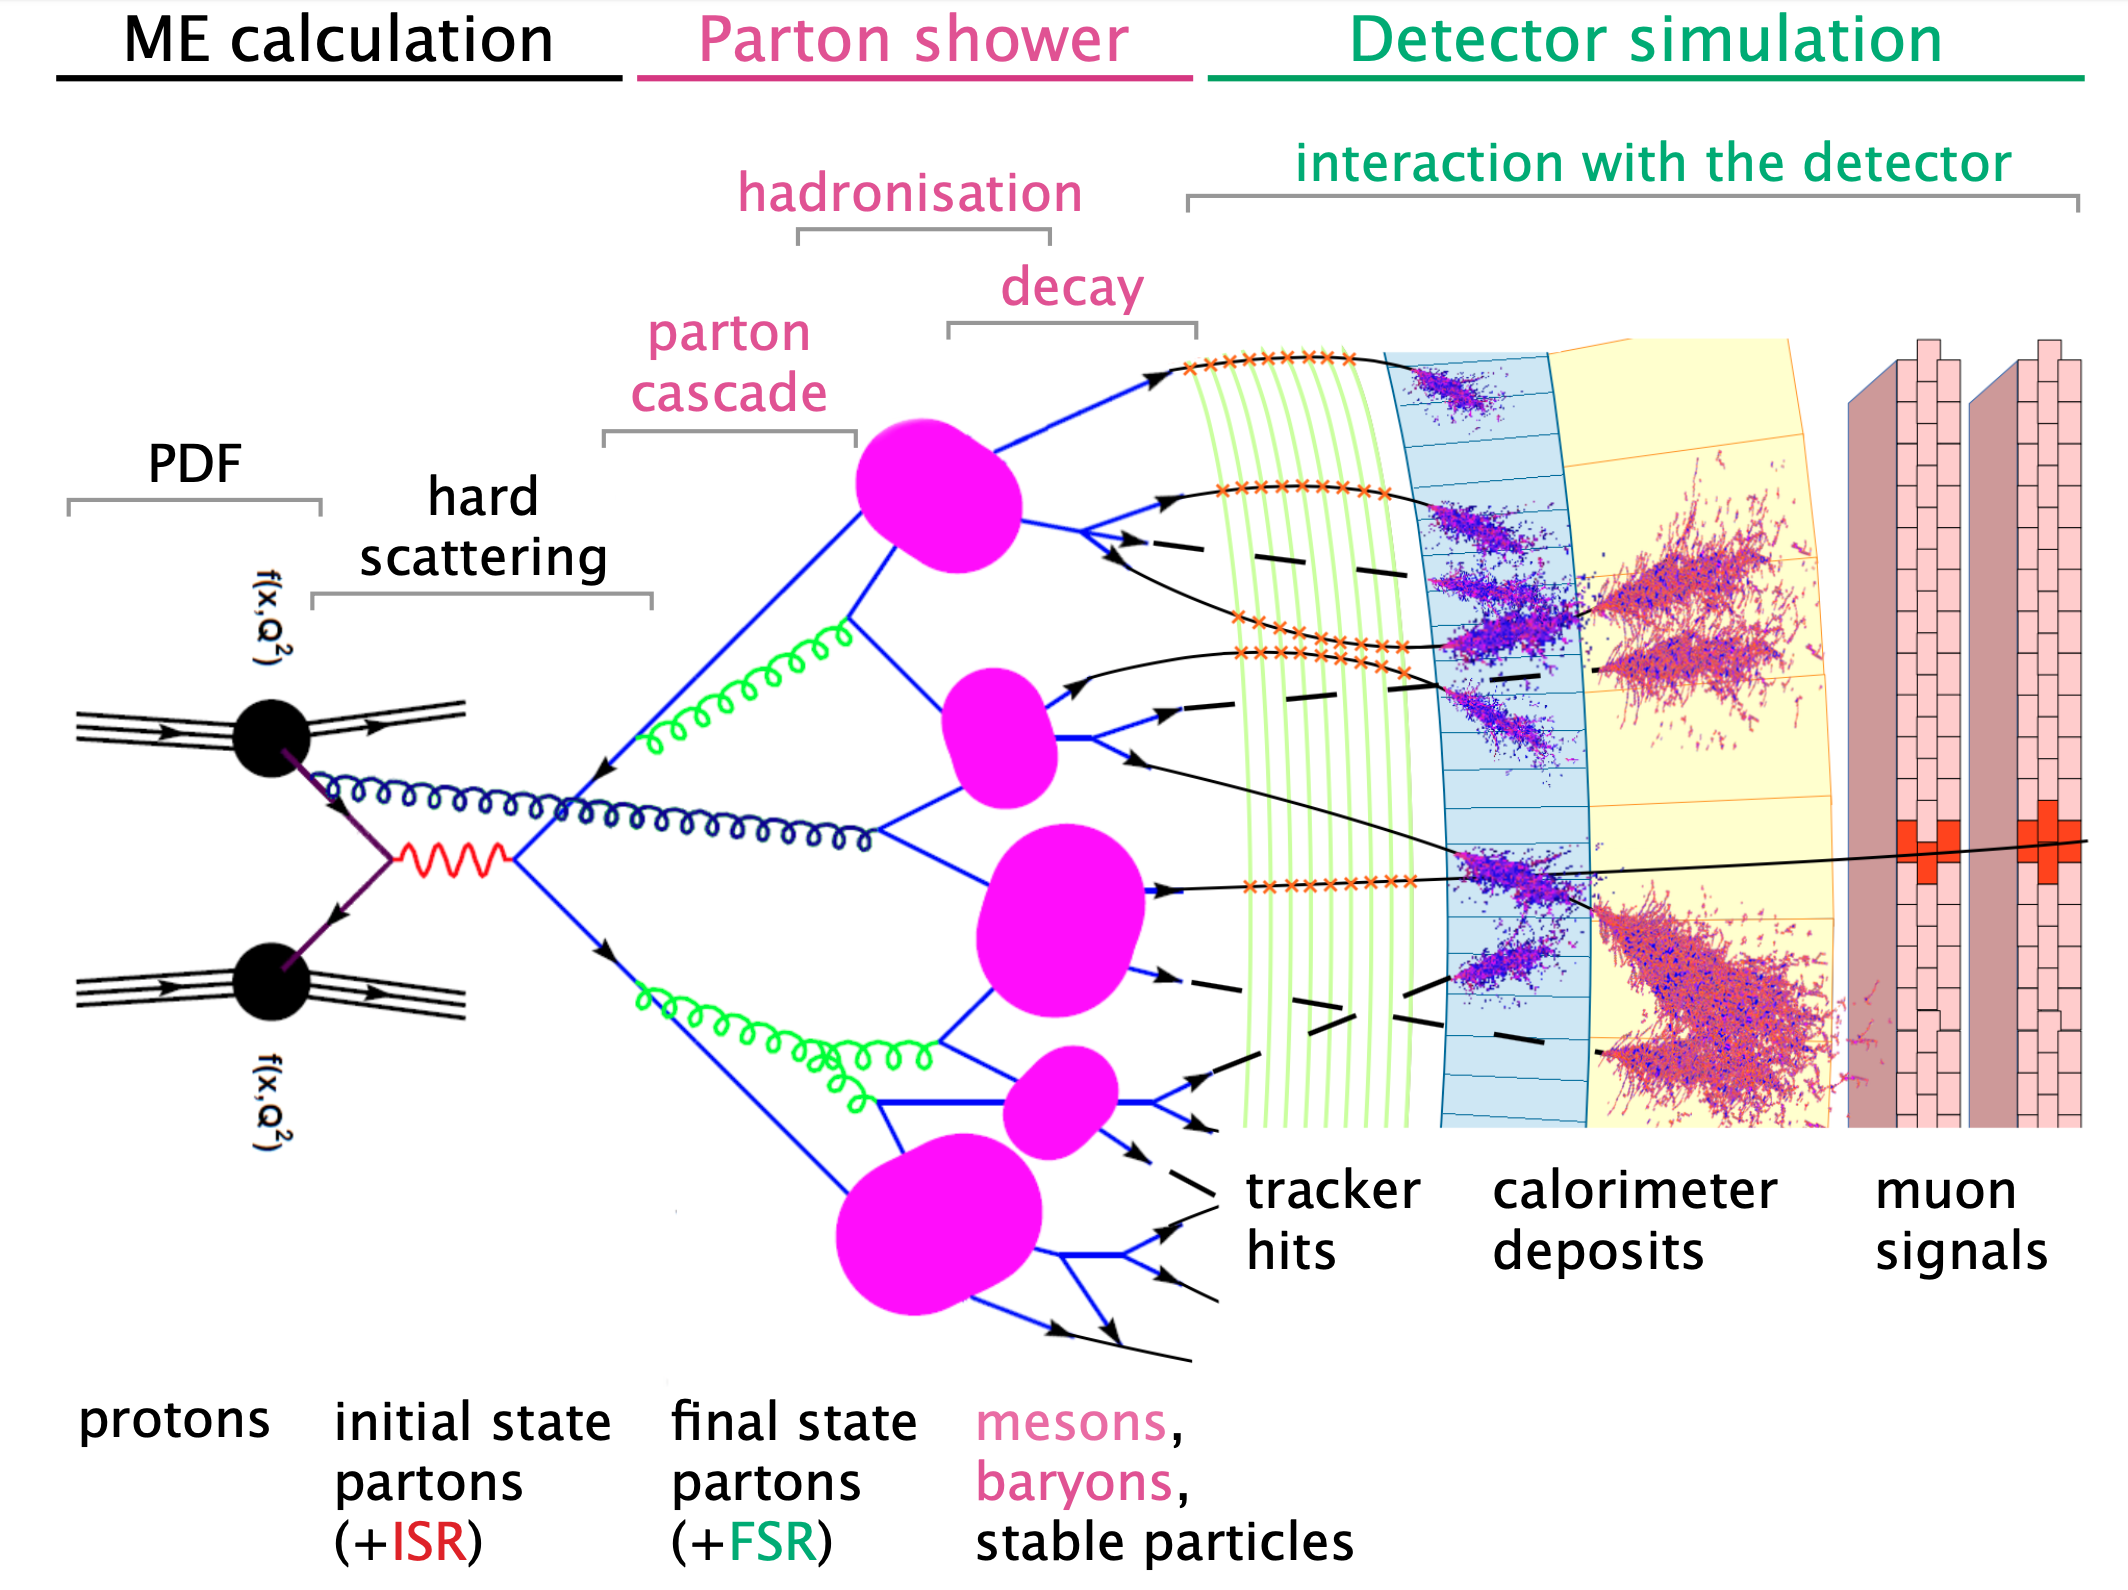
\includegraphics[width=0.9\textwidth]{fig_Event_Simulation/MC_simulation.png}
    \end{tabular}
    \caption{A schematic representation of the different steps of MC simulation for $pp$ collisions~\cite{bartosik}.
            }
    \label{MC_simulation}
  \end{center}
\end{figure}

To minimize statistical uncertainties, MC simulations are usually performed with statistics much higher than in data recorded by the detector, and can be reweighted to match the luminosity of recorded data:
\begin{linenomath*}
\begin{align}
w = \frac{\mathcal{L} \cdot \sigma_{\text{Process}}}{N_{\text{Gen}}}
\end{align}
\end{linenomath*}
where $w$ is the global event weight, $\mathcal{L}$ is the measured integrated luminosity of recorded data, $\sigma_{\text{Process}}$ is the cross-section of the simulated process, and $N_{\text{Gen}}$ is weighted sum of simulated events.

\section{Parton Distribution Functions}
\label{sec:Parton_Distribution_Functions}
For inelastic $pp$ collisions at the LHC, partons within the proton are at sufficient energies to be asymptotically free, and the hard process can be treated as a direct parton-parton interaction.
Protons are composed of not only three valence quarks, but also gluons and a sea of virtual quarks.
The proton parton distribution functions (PDF), shown in figure~\ref{Parton_Distribution_Functions}, give the probability density $f$ of finding a specific parton within the proton with a certain fraction $x$ of the proton's longitudinal momentum at factorization scale $\mu_F$.
\begin{figure}[!htb]
  \begin{center}
    \begin{tabular}{c}
        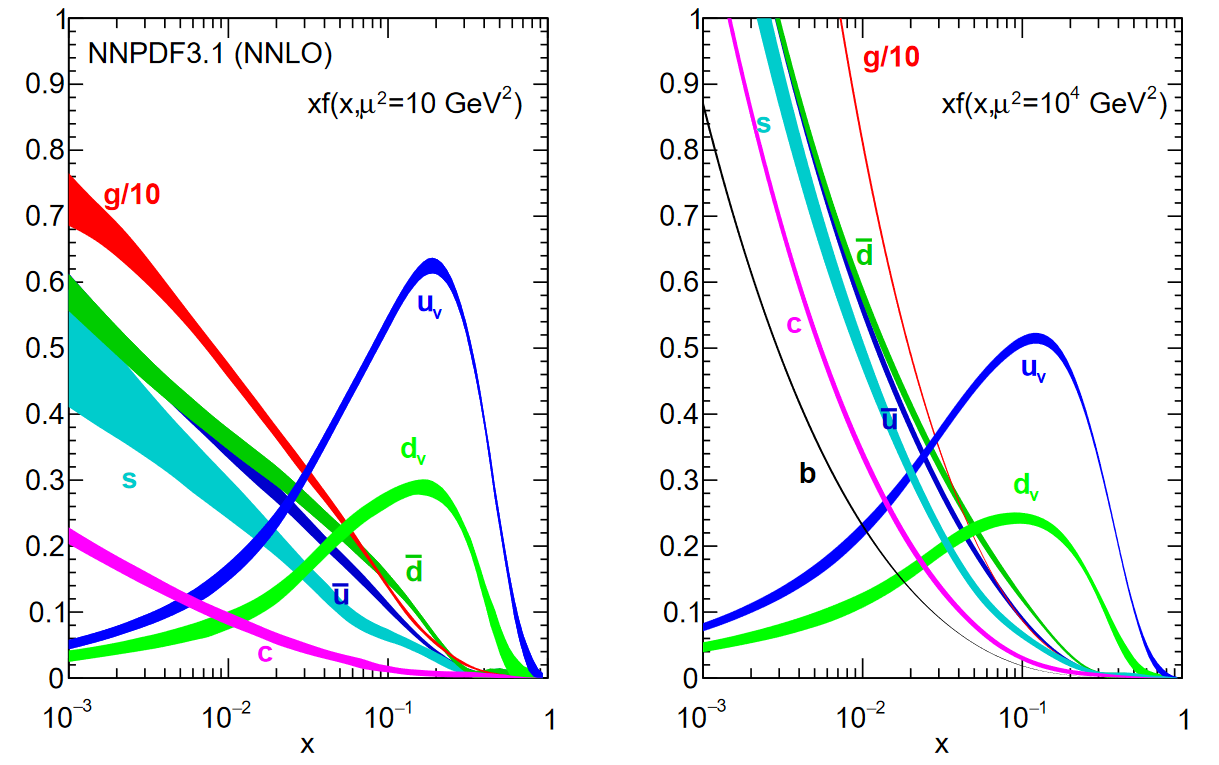
\includegraphics[width=0.80\textwidth]{fig_Event_Simulation/Parton_Distribution_Functions.png}
    \end{tabular}
    \caption{The proton PDF gives the probability density $f$ of finding a specific parton within the proton with a certain fraction $x$ of the proton's longitudinal momentum.
    Shown for scales $\mu_F = \SI{3.1}{\GeV}$ (Left) and at $\mu_F = \SI{100}{\GeV}$ (Right), according to the NNPDF collaboration~\cite{Ball:2267455}.
            }
    \label{Parton_Distribution_Functions}
  \end{center}
\end{figure}
The PDF cannot be calculated from first principles, so it has to be determined experimentally from fitting a combination of data from different types of deep inelastic scattering and hadron collision measurements.
This measurement uses the NNPDF3.1 NLO set of PDFs.

\section{Matrix Element Calculation and Production Cross-section}
\label{sec:Matrix_Element_Calculation_and_Production_Cross-section}
A hard interaction is an event is a process in which heavy objects are created or a large momentum transfer occurs.
For hard parton scattering processes at high energy proton colliders $\alpha_S << 1$, so partonic cross sections can be expanded in a power series expansion of $\alpha_S$ and be calculated in fixed-order perturbation theory. 
Perturbative calculations to accuracies $\mathcal{O}(\alpha^2_S)$, $\mathcal{O}(\alpha^3_S)$, and $\mathcal{O}(\alpha^4_S)$ are referred to as leading-order (LO), next-to-leading-order (NLO), and next-to-next-to-leading-order (NNLO), respectively.
The partonic cross-sections are convoluted with the proton PDFs to obtain $pp$ collision production cross-sections~\cite{BUCKLEY2011145}.
The cross-section or the scattering process $IJ \rightarrow X$ can be expressed as:
\begin{linenomath*}
\begin{align}
\sigma_{IJ \rightarrow X}(s, \mu_F, \mu_R) = \sum_{i, j = g, q, \bar{q}}^{} \int_{0}^{1} \mathrm{~d} x_i \mathrm{~d} x_j f_{\sfrac{i}{I}}\left(x_i, \mu_F^2\right) f_{\sfrac{j}{J}}\left(x_j, \mu_F^2\right) \cdot \hat{\sigma}_{i j \rightarrow X}\left(\hat{s}, \mu_F, \mu_R, \alpha_S\right) \\
=\sum_{i, j=g, q, \bar{q}} \int_{0}^{1} \mathrm{~d} x_i \mathrm{~d} x_j \int \mathrm{~d} \Phi_X f_{\sfrac{i}{I}}\left(x_i, \mu_F^2\right) f_{\sfrac{j}{J}}\left(x_j, \mu_F^2\right) \cdot \frac{1}{2 \hat{s}}\left\vert \mathcal{M}_{i j \rightarrow X}\right\vert^2\left(\Phi_X, \mu_F, \mu_R, \alpha_S\right)
\label{ttbar_crosssection}
\end{align}
\end{linenomath*}
where $i(j)$ are the parton constituents of proton $I(J)$, $f_{{\sfrac{i}{I}}({\sfrac{j}{J}})}$ are the parton $i(j)$ PDF of proton $I(J)$, $x_{i(j)}$ are the parton $i(j)$ momentum fraction of proton $I(J)$, $\mu_F$ is the factorization scale, $\mu_R$ is the renormalization scale, $\sigma_{i j \rightarrow X}$ are the exclusive partonic cross-sections for $X$ production, $\hat{s} = s \cdot x_i \cdot x_j$ is the squared center-of-mass energy of the parton collision, \beamenergy is the center-of-mass energy of the proton-proton collision, $\alpha_S$ is the coupling constant of the strong interaction, $\Phi_X$ is the final state phase space, and $\left\vert \mathcal{M}_{i j \rightarrow X}\right\vert^2$ is the matrix element (ME) squared.
The factorization scale $\mu_F$ is conventionally set to the energy scale of the high-energy protons in the collision.
The renormalization scale $\mu_R$ is the arbitrarily chosen high-energy cutoff for the renormalization procedure, used in perturbation theory to separate divergences from higher order corrections.
The ME are calculated by summing over the contributions from the relevant fix-order Feynman diagrams ($\mathcal{M}_{i j \rightarrow X}=\sum_k \mathcal{F}_{i j \rightarrow X}^{(k)}$), summing over the outgoing spin and color quantum numbers, and averaging over the incoming ones.
At LO, ME calculations only include the interaction between incoming partons, but higher order ME calculations will additionally include real emission and virtual loop corrections.
The real emission corrections correspond to radiated partons, which are classified as initial state radiation (ISR) and final state radiation (FSR) depending on whether they are emitted by the incoming or outgoing particles.
This measurement uses the Positive Weight Hard Event Generator v2 (\Powheg) event generator, which perform ME calculations with NLO accuracy and accounts for polarizations in \ttbar production and top quark decays.

\section{Parton Shower}
Parton shower (PS) models account for higher order QCD and QED radiative emissions beyond the accuracy of fixed order perturbative approximations.
Showers of outgoing partons are created as partons radiate gluons and gluons radiate other gluons or produce $q\bar{q}$ pairs.
In this measurement, the PS is modelled using (\Pythia).
In \Pythia\ the radiative emissions are modeled as a Markov chain, where each emission is treated as independent, with the probability of an additional emission being determined by the splitting functions and the kinematics of the partons involved~\cite{pythia8.3}.
The algorithm continues to iteratively split the partons in a cascade of emissions until they reach an energy scale where perturbation theory breaks down.

A matching and merging procedure is used to avoid double-counting radiative emissions from the ME calculation and the PS models~\cite{StefanoFrixione_2007}.
Two general NLO matching methods exist, namely $\textsc{Powheg}$ and $\textsc{Mc@NLO}$, available in $\Powheg$ and automated in $\MGaMCatNLOOnly$ respectively~\cite{pythia8.3}.
In \Powheg, the $h_{damp}$ parameter controls the matching procedure by modifying the scale at which radiative emissions from the PS are discarded in favor of the ME calculations.
Lower (higher) values of $h_{damp}$ result in softer (harder) radiated emissions and less (more) events with high \pT jets.
$\textsc{MLM}$ and $\textsc{UMEPS}$ are tree-level methods for merging, while $\textsc{FxFx}$, which combines $\textsc{Mc@NLO}$ matching with $\textsc{MLM}$ matching, and $\textsc{UNLOPS}$, which is an extension of $\textsc{UMEPS}$, are for NLO merging~\cite{pythia8.3}.
$\textsc{UNLOPS}$ is the preferred NLO merging scheme in \Pythia, but the $\textsc{FxFx}$ procedure is used for NLO MC simulations when when the ME calculations were performed by $\MGaMCatNLOOnly$.

For $pp$ collisions, besides the parton interaction in the hard process, the remaining constituent partons of the colliding protons, referred to as the beam-beam remnants (BBR), can also interact.
These multiple parton interactions (MPI) can produce additional independent scattering processes that contribute to the underlying event (UE).
Pileup (PU) additionally 
PS models in event generators have a adjustable parameters to control the behavior of event modeling, and a set of these parameters, which has been adjusted to better fit some aspects of the data, is referred to as a UE tune~\cite{Sirunyan:2669320}.
The CP5 UE tune was chosen for all simulated samples for this measurement.

\section{Hadronization}
Hadronization is the direct consequence of color confinement and the running of $\alpha_S$ at low energy scales where QCD is non-perturbative.
As non-perturbative QCD is unsolved, hadronization is simulated using phenomenological models that describe the process of forming colorless hadrons from quarks and gluons.
In \Pythia, it is based on the Lund string model, which assumes that the potential energy of color charge dipole fields grows linearly ($V(r) = \kappa r$ with $\kappa \approx \SI{1}{\GeV \per \femto \m}$) with the separation of the charges~\cite{SJOSTRAND2015159}.
As color charges ($q$ and $\bar{q^\prime}$) separate, the potential energy increases beyond the threshold that the color flux tube snaps and a new color charge pair ($q^\prime$ and $\bar{q^\prime}$) emerges.
After the snap, the system consists of two separate color charge dipole fields ($q\bar{q^{\prime\prime}}$ and $q^{\prime\prime}\bar{q^\prime}$).
Further snaps continue until the potential energy of the tubes are not sufficient to produce new color charge pairs.

In these models, individual partons do not hadronize independently, but rather colour-connected systems of partons hadronize collectively~\cite{BUCKLEY2011145}.
The scenario in which color fields connecting different partons rearrange themselves after the collision and before the formation of final hadrons is referred to as color reconnection (CR).
To more accurately describe the data, phenomenological CR models are used to simulate color-flow.
\Pythia\ uses a MPI-based CR scheme in which there is a probability that the partons of the lower-\pT proton are added to the strings defined by the higher-\pT proton in such a way as to give the smallest total string length.

\section{Detector Response}
The interaction of the MC generated final state particles with the CMS detector are simulated with the GEometry ANd Tracking (\Geant v10.4.3) toolkit.
\Geant\ divides the the trajectory of particles traversing the detector into small, finite steps and calculates the probability that the particles will interact with the material in the detector based on their properties and the properties of the material they are passing through~\cite{AGOSTINELLI2003250}.
A complete set physics models for the electromagnetic, strong and weak interactions are included in \Geant.
If an interaction occurs, \Geant\ calculates the resulting energy deposition, generates any secondary particles that are produced, and simulates the response of the readout electronics and trigger system including the effects of noise and other sources of background.
To provide an accurate simulation, \Geant\ uses a detailed description of the detector geometry and materials, calibrations, and electronics performance including dead channels.
Experimental data is used to parameterize detector response and validate the simulation~\cite{Bayatian:922757}.
The collection of \Geant-simulated detector responses for an event is stored in the raw CMS event data model (EDM) format and can be reconstructed exactly as actual events recorded by the CMS detector.
\ProvidesFile{chapters/ch-Event_Selection.tex}

\chapter{Datasets, Event Selection, and Kinematic Reconstruction}
\label{Datasets_Event_Selection_Kinematic_Reconstruction}
The signal process for this measurement is the production of top quark pairs followed by top quark decays $t\to W^+ b$ and $\bar{t}\to W^- \bar{b}$, and subsequent leptonic W boson decays into final state muons $W\to \mu\nu$ and electrons $W\to e\nu$, both "prompt" and "via tau", i.e. via the decay of the W boson into a tau $W\to \tau\nu$ and its subsequent leptonic decay into a final state electron $\tau\to e\nu$ or muon $\tau\to \mu\nu$.
The analysis has been carried out using the CMS EDM and official software framework for event generation, simulation, and reconstruction, following recommendations for ultra-legacy Run II analyses by the Physics Performance and Datasets (PPD) and the Physics Data And Monte Carlo Validation (PdmV) CMS groups.

\section{Datasets}

\subsection{Recorded Datasets}
This measurement is performed using \lumivalueSixPreVFP $\pm$ \lumierrSixPreVFP~\cite{bib:lumipas16}, \lumivalueSixPostVFP $\pm$ \lumierrSixPostVFP~\cite{bib:lumipas16}, \lumivalueSeven $\pm$ \lumierrSeven~\cite{bib:lumipas17}, and \lumivalueEight $\pm$ \lumierrEight~\cite{bib:lumipas18} (Total: \lumivalueRuniiUL $\pm$ \lumierrRuniiUL) of data collected with the CMS experiment at the LHC with \beamenergy, during 2016, 2017, and 2018 respectively.
Only the runs and luminosity sections that had good functioning of every CMS sub-detector were selected for analysis.

\subsection{Simulated Datasets}
MC simulations are used to estimate signal and background contributions. 
The dileptonic \ttbar signal sample is produced using the \Powheg\ event generator with NLO ME calculations. 
PS and hadronization of the \ttbar signal sample is performed using \Pythia. 
The matrix-element jets are matched to parton showers using the \Powheg\ method. 
The MC simulations assume that $m_t = \SI{172.5}{\GeV}$, and the PDFs are described using NNPDF3.1.
\Powheg\ assumes that the \ttbar branching fractions are flavor-independent with flavor-averaged branching fractions of $0.1091$, so correction factors were calculated and applied to correct each dilepton channel to the flavor-specific PDG value.
The following flavor-specific branching fractions are taken from PDG~\cite{bib:PDG}: $b_{{\ensuremath{W\to e\nu}}} = 0.1071$ $\pm$ 0.0016, $b_{{\ensuremath{W\to \mu\nu}}} = 0.1063$ $\pm$ 0.0015, and $b_{{\ensuremath{W\to \tau\nu}}} = 0.1138$ $\pm$ 0.0021.
The branching fraction of $\tau$ leptons decaying into a muon is given by $b_{{\ensuremath{\tau\to \mu\nu\nu}}} = 0.1741$ $\pm$ 0.0004 and for taus decaying to an electron it is $b_{{\ensuremath{\tau\to e\nu\nu}}} = 0.1783$ $\pm$ 0.0004.
The following \ttbar dilepton branching fraction global correction factors were applied per prompt dilepton channel: $\mathcal{C}_{\ee} = 0.964261576$, $\mathcal{C}_{\emu} = 0.957058875$, and $\mathcal{C}_{\mumu} = 0.949909976$.  
\ttbar dilepton events with at least one leptonic tau decay are considered as signal in this analysis and the following branching fraction global correction factors were applied per dilepton channel via tau: $\mathcal{C}_{\ee} = 1.029827957$, $\mathcal{C}_{\emu} = 1.026209047$, and $\mathcal{C}_{\mumu} = 1.022670477$.

The major sources of background contributions are semi-leptonic \ttbar, fully hadronic \ttbar, dileptonic decays of single top quarks in association with a $W$ boson ($tW$ and $\bar{t}W$), \ttbar in association with $W/Z$ bosons, \zjets, \wjets, and $WW$, $WZ$, $ZZ$ diboson processes. 
A summary of the MC simulated process for background processes is shown in table~\ref{simulated_Datasets}, including the ME generator, PS algorithm, and cross-section used for luminosity scaling.

\begin{table}[!htb]
 \begin{center}
   \begin{adjustbox}{scale=0.75,center}
    \begin{tabular}
      {lccr} \hline Process & ME (Matching) & PS & $\sigma$ [pb]\\
      \hline
      { \ttbar (Dileptonic)} & \Powheg & \Pythia &  $\xsecTTBARdilept$ \\
      { \ttbar (Semi-Leptonic)} & \Powheg & \Pythia &  $\xsecTTBARljets$ \\
      { \ttbar (Hadronic)} & \Powheg & \Pythia &  $\xsecTTBARhadronic$ \\
      { $\ttbar+W$ (Leptonic $W$)} & \MGaMCatNLOOnly+\MadSpin & \Pythia &  $\xsecTTWJETSlnu$ \\
      { $\ttbar+W$ (Hadronic $W$)} & \MGaMCatNLOOnly+\MadSpin & \Pythia &  $\xsecTTWJETSqq$ \\
      { $\ttbar+Z$ (Leptonic $Z$)} & \MG & \Pythia &  $\xsecTTZllnunu$ \\
      { $\ttbar+Z$ (Hadronic $Z$)} & \MG & \Pythia &  $\xsecTTZqq$ \\
      { $t+W$ (Dileptonic)} & \Powheg & \Pythia &  $\xsecSINGLETOPtw$ \\
      { $\bar{t}+W$ (Dileptonic)} & \Powheg & \Pythia &  $\xsecSINGLETOPtw$ \\
      { $W+\text{Jets}$} & \MG & \Pythia &  $\xsecWlnu$ \\
      { $Z/\gamma^*+\text{Jets} \quad (\SI{10}{\GeV} < m_{\ell\bar{\ell}} < \SI{50}{\GeV})$} & \MG & \Pythia &  $\xsecDYTenFifty$ \\
      { $Z/\gamma^*+\text{Jets} \quad (\SI{50}{\GeV} < m_{\ell\bar{\ell}})$} & \MG & \Pythia &  $0.5 \times \xsecDYFiftyInf$ \\
      { $Z/\gamma^*+\text{Jets} \quad (\SI{50}{\GeV} < m_{\ell\bar{\ell}})$} & \MGaMCatNLO & \Pythia &  $0.5 \times \xsecDYFiftyInf$ \\
      { $WW$} & \Pythia & \Pythia &  $\xsecWW$ \\
      { $WZ$} & \Pythia & \Pythia &  $\xsecWZ$ \\
      { $ZZ$} & \Pythia & \Pythia &  $\xsecZZ$ \\
      \hline
      \end{tabular}
   \end{adjustbox}
  \caption{}
  \label{simulated_Datasets}     
 \end{center}
\end{table}

\section{Event Selection and Simulation Corrections}
The \ttbar dilepton final state is characterized by the presence of at least two high-\pT isolated leptons with opposite electric charge, large MET (\ETmiss), and two jets created from the hadronization of $b$-quarks.
The reconstruction of the different objects is performed using the PF algorithm.
The object identification criteria follow the recommendations for ultra-legacy Run II analyses by the CMS Top Physics Analysis Group (Top PAG).

\subsection{Triggers}
To maximize the trigger efficiency, dilepton data streams and single lepton streams are both used for this measurement.
In order to ensure no double-counting of events, events passing the dilepton triggers are vetoed when processing the single lepton data streams.
Approximately 10\% of dilepton events that failed to pass the dilepton trigger requirements are recovered by including the single lepton data streams.
The trigger efficiency is measured in data as a function of the lepton $\pT$ and used to correct the MC simulations.

\subsection{Primary Vertex Requirements and Pileup Corrections}
The PV of an event is required to associated with at least four tracks and be in the vicinity of the nominal interaction point with $\vert r \vert < \SI{2}{\cm}$ and $\vert z \vert < \SI{24}{\cm}$. 
Charged-hadron subtraction (CHS) is used to remove charged PU contributions and the L1FastJet algorithm is applied to subtract the remaining neutral contributions.
The number of PU events in MC simulations is typically based on an estimate of the expected number of interactions per bunch crossing and PU reweighting is performed using the instantaneous luminosity per bunch crossing in data, and the total $pp$ inelastic cross section of $\SI{69.2}{\m \b}$, to correct the PU distribution of the MC simulation.

\subsection{Muons}
PF muon candidates are required to have a transverse momentum $\pT > \SI{20}{\GeV}$ and a pseudorapidity restricted to the coverage of the inner tracker $\vert \eta \vert < 2.4$.
They are also required to be reconstructed as global muons and fulfill tight selection criteria: 
\begin{itemize}
    \item at least six hits in the tracker layers
    \item at least one hit in the pixel detector
    \item muon segments in at least two muon stations
    \item at least one muon-chamber hit included in the global-muon track fit
    \item $\chi^2/ndof < 10$ for the global muon fit
    \item its track has transverse impact parameter $d_xy< \SI{2}{\mm}$ and longitudinal distance $d_z< \SI{5}{\mm}$ with respect to the primary vertex
\end{itemize}
These criteria suppress hadronic "punch-through" fake-muons and muons produced in hadron decays to ensure high purity and provide good $\pT$ measurements.
To remove leptons overlapping with jets, PF muon candidates are required to fulfill the isolation condition $I^{PF}_{Rel}< 0.15$, where $I^{PF}_{Rel}$ is calculated as: 
\begin{linenomath*}
\begin{align}
I^{PF}_{Rel} = \frac{1}{\pT(\mu)}(I_\mathrm{CH} + \max(0, I_\mathrm{N} + I_\mathrm{PH} - 0.5 I_\mathrm{CH,pu}))
\end{align}
\end{linenomath*}
and divided by the \pT of the muon.
It is the \pT-sum of charged (CH), neutral (N), and photon-like (PH) transverse energy deposits from charged hadron, neutral hadron and photon PF candidates, relative to the \pT of the muon, inside a cone, in $\eta$-$\phi$ space, of $\Delta R < 0.4$ around the muon.
$I_\mathrm{CH,pu}$ is the sum over charged PF candidates not originating from the main primary vertex and its subtraction compensates for PU contributions. 
Corrections are also applied that scale the raw energy measurements and smear the muon resolutions to match the accuracy and precision of reconstructed muons in MC simulation to those in recorded data.
Identification and isolation efficiency corrections for muons are also applied, and are measured as a function of \pT and $\eta$ using a "tag-and-probe" method with an orthogonal dataset.

\subsection{Electrons}
PF electron candidates are required to have transverse momentum $\pT > \SI{20}{\GeV}$ and a pseudorapidity restricted to the coverage of the inner tracker $\vert \eta \vert < 2.4$.
The gap between the barrel and endcap region of the ECAL ($1.4442 < \vert \eta_\mathrm{sc} \vert < 1.5660$) is excluded, where $\eta_\mathrm{sc}$ is the pseudorapidity of the ECAL supercluster.
To ensure high purity, the electron selection uses tight identification and isolation criteria.
The electron isolation considers photons $\gamma$, neutral hadrons $\mathrm{nh}$, and charged hadrons $\mathrm{ch}$ as identified by the PF algorithm in a cone, in $\eta$-$\phi$ space, of $\Delta R < 0.3$ around the electron.
The relative isolation is calculated as: 
\begin{linenomath*}
\begin{align}
I^{PF}_{Rel} = I_{\mathrm{ch}} + \max(I_\gamma + I_{\mathrm{nh}} - \rho A_{\mathrm{eff}}, 0)
\end{align}
\end{linenomath*}
and divided by the \pT of the electron.
$A_{eff}$ is an $\eta$ dependent effective area that gives information about the susceptibility to soft contamination and is chosen such that isolation is flat with respect to the number of PU interactions. 
It is used in combination with $\rho$, which is an estimate of the energy density per unit area contributed by PU interactions, to subtract energy deposition from PU interactions from the isolation.
$\rho$, the energy deposition per area due to unclustered objects, is estimated from the fixed grid approach and the $\rho A_{eff}$ term ensures that the isolation efficiency is almost independent of the PU conditions.
Corrections are also applied that scale the raw energy measurements and smear the electron resolutions to match the accuracy and precision of reconstructed electrons in MC simulation to those in recorded data.
Identification and reconstruction efficiency corrections for electrons are also applied, and are measured as a function of \pT and $\eta$ using a "tag-and-probe" method with an orthogonal dataset.

\subsection{Lepton Pair}
Events with a dilepton system consisting of exactly two oppositely-charged leptons passing the electron and muon object selection criteria are accepted for further consideration.
If more than two leptons are reconstructed in the event, then the event is vetoed.
The leading selected lepton is required to have $\pT > \SI{25}{\GeV}$.
The event is then unambiguously classified as \ee, \emu, or \mumu depending on the type of the selected lepton pair, and the event is discarded if there are additional leptons in the event, other than the two which enter the defined lepton pair.
The invariant mass of the selected lepton pair is required to be larger than $\SI{20}{\GeV}$ to suppress background events from decays of heavy-flavour resonances and Drell-Yan processes.
Moreover, in the \mumu and \ee decay channels, events are rejected if the dilepton invariant mass is within the vicinity of the $Z$ boson mass $\SI{76}{\GeV} < m_{\ell\bar{\ell}} < \SI{106}{\GeV}$, where background from $Z$ boson production is dominant.

\subsection{Jets}
Jets are clustered from reconstructed PF candidates using the anti-$k_T$ clustering algorithm with radius parameter $R = 0.4$ (AK4).
Events are required to have at least two jets with transverse momentum $\pT > \SI{30}{\GeV}$ and within the coverage of the inner tracker $\vert \eta \vert < 2.4$. 
The following identification criteria is applied to efficiently identify jets (efficiency \sim $98\% - 99\%$) while rejecting jets with significant lepton fractions (purity \sim $98\%$) :
\begin{itemize}
\item Neutral Hadron Fraction $<0.9$
\item Neutral EM Fraction $<0.9$
\item Number of Constituents $>1$
\item Muon Fraction $<0.8$
\item Charged Hadron Fraction $>0$
\item Charged Multiplicity $> 0$
\item Charged EM Fraction $<0.8$ 
\end{itemize}
Additionally, a cleaning of leptons from jets is applied if $\Delta R(jet,lepton)<0.4$, to exclude jets overlapping with selected leptons used in the analysis.
Events with jets in regions of the calorimeter that produced anomalously high or low jet rates are vetoed in MC and recorded data.

Jet energy corrections (JEC) are applied that adjust the jet energy scale (JES) to match the accuracy of reconstructed jet energies in MC simulation to those in recorded data.
To reduce the contribution coming from PU, the CHS algorithm removes charged particles and the L1FastJet algorithm removes the remaining neutral contributions from PU vertices before clustering jets~\cite{bib:JME18001}.
L2L3 MC-truth corrections are applied to both data and MC simulation to correct for the variation of detector resolution as a function of jet $\eta$ and \pT.
Any remaining discrepancies in the accuracy of jet energy measurements due to detector response and other effects are eliminated with the application of L2L3Residual corrections.
Jet energy resolution (JER) corrections are applied by smearing the jets in MC simulation to match the precision of jets in recorded data.

\subsection{Missing Transverse Energy}
The calculation of the MET (\ETmiss) is based on PF objects, where PU-per-particle-identification (PUPPI)~\cite{bib:PUPPI} is used for PU mitigation.
PUPPI is an alternative to the PF CHS algorithm which gives weights to particles based on the probability that they come from PU or the PV.
The JEC (JES and JER) and lepton energy scale corrections are propagated to the \ETmiss.
Events in the \mumu and \ee channels are required to have $\ETmiss > \SI{40}{\GeV}$, but no requirement on \ETmiss is applied in the \emu channel.

\subsection{Tagging of b-Jets}
Selected events are required to have at least one jet tagged as having originate from a $b$-quark.
In this analysis, the DeepJet $b$-tagging algorithm~\cite{bib:Bols_2020}, which uses uses approximately 650 input variables, divided into four categories (global variables, charged PF candidate features, neutral PF candidate features, and secondary vertex features associated with the jet) as inputs for a deep neural network, is used to tag all reconstructed jets in the event.
In this analysis, a DeepJet medium working point is used with light ($l$)-jet mistag efficiency of \sim$1\%$.

Due to the differences between $b$-tagging algorithm efficiencies in recorded data and MC simulation, MC simulated events are reweighted with corrective scale factors after selection.
Data-to-simulation corrective scale factors ($\mathcal{SF}_{BTV}$) for the $b$-tagging efficiency of individual $b$-jets, and \textit{mistag rate} $c$-jets and light-($l$) jets, are measured with an orthogonal QCD multi-jet dataset and parameterized as a function of the jet \pT.
To correct the possible differences of the b-tagging efficiency due to the different kinematics of the \ttbar events and the QCD multijet events used to measure the data-to-simulation corrective scale factors, the $b$-tagging efficiency ($\mathcal{E}_{MC}$) of $b$-jets and mistag rate for $c$- and $l$-jets, which do not only depend on the jet kinematic properties but also on the event selection, are estimated in this analysis using the MC simulated \ttbar signal events.
The probability $P$ of a given configuration of jets in MC simulation and data is defined as:
\begin{linenomath*}
\begin{align}
P(MC) = \prod_{\substack{i=tagged}} \mathcal{E}_i \prod_{\substack{j=not~tagged}} (1 - \mathcal{E}_j) \\
P(Data) = \prod_{\substack{i=tagged}} \mathcal{SF}_i\mathcal{E}_i \prod_{\substack{j=not~tagged}} (1 - \mathcal{SF}_j\mathcal{E}_j),
\end{align}
\end{linenomath*}
where $\mathcal{E}_i$ and $ \mathcal{SF}_i $ refer respectively to $\mathcal{E}_{MC}$ and $\mathcal{SF}_{BTV}$, which are functions of the jet flavor, jet \pT, and jet $\eta$. 
Afterwards, the event weight is computed accordingly to $\mathcal{W}_{b-tag} = \frac{P(Data)}{P(MC)}$.


\section{\ensuremath{\mathrm{t\bar{t}}} Kinematic Reconstruction}

\subsection{Full \ensuremath{\mathrm{t\bar{t}}} Kinematic Reconstruction}
To fully pass event selection, an event is also required to have at least one solution to the \ttbar kinematic reconstruction.
The top quark and anti-quark are fully reconstructed using an analytical method~\cite{Sonnenschein:2006ud}, in which eight kinematic constraints are applied to determine the unknown four-momenta of the undetected neutrinos.
The constraint equations are constructed from the four-momenta of the objects passing event selection: two leptons, two jets, and the missing transverse energy. 
The two neutrinos are assumed to be massless $m_{\nu} = m_{\bar{\nu}} = \SI{0}{\GeV}$:
\begin{linenomath*}
\begin{align}
m_{\nu}^2 = E_{\nu}^2 - p_{x, \nu}^2 - p_{y, \nu}^2 - p_{z, \nu}^2 \\
m_{\bar{\nu}}^2 = E_{\bar{\nu}}^2 - p_{x, \bar{\nu}}^2 - p_{y, \bar{\nu}}^2 - p_{z, \bar{\nu}}^2 
\end{align}
\end{linenomath*}
The missing transverse energy is assumed to be entirely from the transverse momenta of the two neutrinos:
\begin{linenomath*}
\begin{align}
E_{x}^{\text{miss}}=p_{x, \nu}+p_{x, \bar{\nu}} \\
E_{y}^{\text{miss}}=p_{y, \nu}+p_{y, \bar{\nu}}
\end{align}
\end{linenomath*}
The lepton (anti-lepton) and the anti-neutrino (neutrino) are assumed to have an invariant mass equal to the W boson mass of $m_{W^\pm} = \SI{80.4}{\GeV}$:
\begin{linenomath*}
\begin{align}
m_{W^{+}}^2 =\left(E_{\bar{\ell}}+E_\nu\right)^2-\left(p_{x, \bar{\ell}}+p_{x, \nu}\right)^2  -\left(p_{y, \bar{\ell}}+p_{y, \nu}\right)^2-\left(p_{z, \bar{\ell}}+p_{z, \nu}\right)^2 \\
m_{W^{-}}^2 =\left(E_{\ell}+E_{\bar{\nu}}\right)^2-\left(p_{x, \ell}+p_{x, \bar{\nu}}\right)^2 -\left(p_{y, \ell}+p_{y, \bar{\nu}}\right)^2-\left(p_{z, \ell}+p_{z, \bar{\nu}}\right)^2
\end{align}
\end{linenomath*}
Finally, the reconstructed top quark and anti-quark are assumed to have an invariant mass of $m_{t} = m_{\bar{t}} = \SI{172.5}{\GeV}$:
\begin{linenomath*}
\begin{align}
m_t^2 =\left(E_{\bar{\ell}}+E_\nu+E_b\right)^2-\left(p_{x, \bar{\ell}}+p_{x, \nu}+p_{x, b}\right)^2 -\left(p_{y, \bar{\ell}}+p_{y, \nu}+p_{y, b}\right)^2-\left(p_{z, \bar{\ell}}+p_{z, \nu}+p_{z, b}\right)^2 \\
m_{\bar{t}}^2 =\left(E_{\ell}+E_{\bar{\nu}}+E_{\bar{b}}\right)^2-\left(p_{x, \ell}+p_{x, \bar{\nu}}+p_{x, \bar{b}}\right)^2 -\left(p_{y, \ell}+p_{y, \bar{\nu}}+p_{y, \bar{b}}\right)^2-\left(p_{z, \ell}+p_{z, \bar{\nu}}+p_{z, \bar{b}}\right)^2
\end{align}
\end{linenomath*}
The constraint equations can be simplified to a single $4^{\text{th}}$ order polynomial equation for one of the neutrino four-momenta components, which can be solved analytically with up to a four-fold ambiguity to obtain the neutrino and top quark four-momenta.
If an event may contain more than two b-jet candidates, then each pair of jet--lepton assignments are tried.
Jets b-tagged by the DeepJet algorithm are tried first, and only if no solution is found are the untagged jets considered.
The solution which yields the minimum invariant mass of the \ttbar system has been shown~\cite{PhysRevD.73.112006} to, in most cases, provide the solution with correct jet--lepton assignments and is the method used in this measurement to resolve the ambiguities arising from having multiple solutions.

Due to fluctuations in the measured jet momenta and missing transverse energy, the simplified constraint equation is not always solvable.
To enhance reconstruction efficiency, each event is reconstructed 100 times with a different random smearing of jet and lepton energies and directions within their resolutions.
The resolutions are determined using the signal MC simulation after event selection by comparing the reconstructed jet and lepton energies and directions to the true b-quark and lepton values.
The jet and lepton energies are smeared by randomly sampling a distribution of the ratio of the true energy divided by the reconstructed energy (the ratio distributions are shown in figure~\ref{fig:energyFactor}).
The directions are smeared randomly about the reconstructed direction with magnitude sampled from a Gaussian distribution with resolution taken from the average of the angular difference between the reconstructed and true directions (the distributions from which the average resolutions were obtained are shown in figure~\ref{fig:angleFactor}).
The $W$ boson masses used in the constraints are also smeared randomly about their central values using the width of their relativistic Breit-Wigner mass distribution (shown in figure~\ref{fig:inputDists}).

\begin{figure}[!htb]
    \begin{center}
        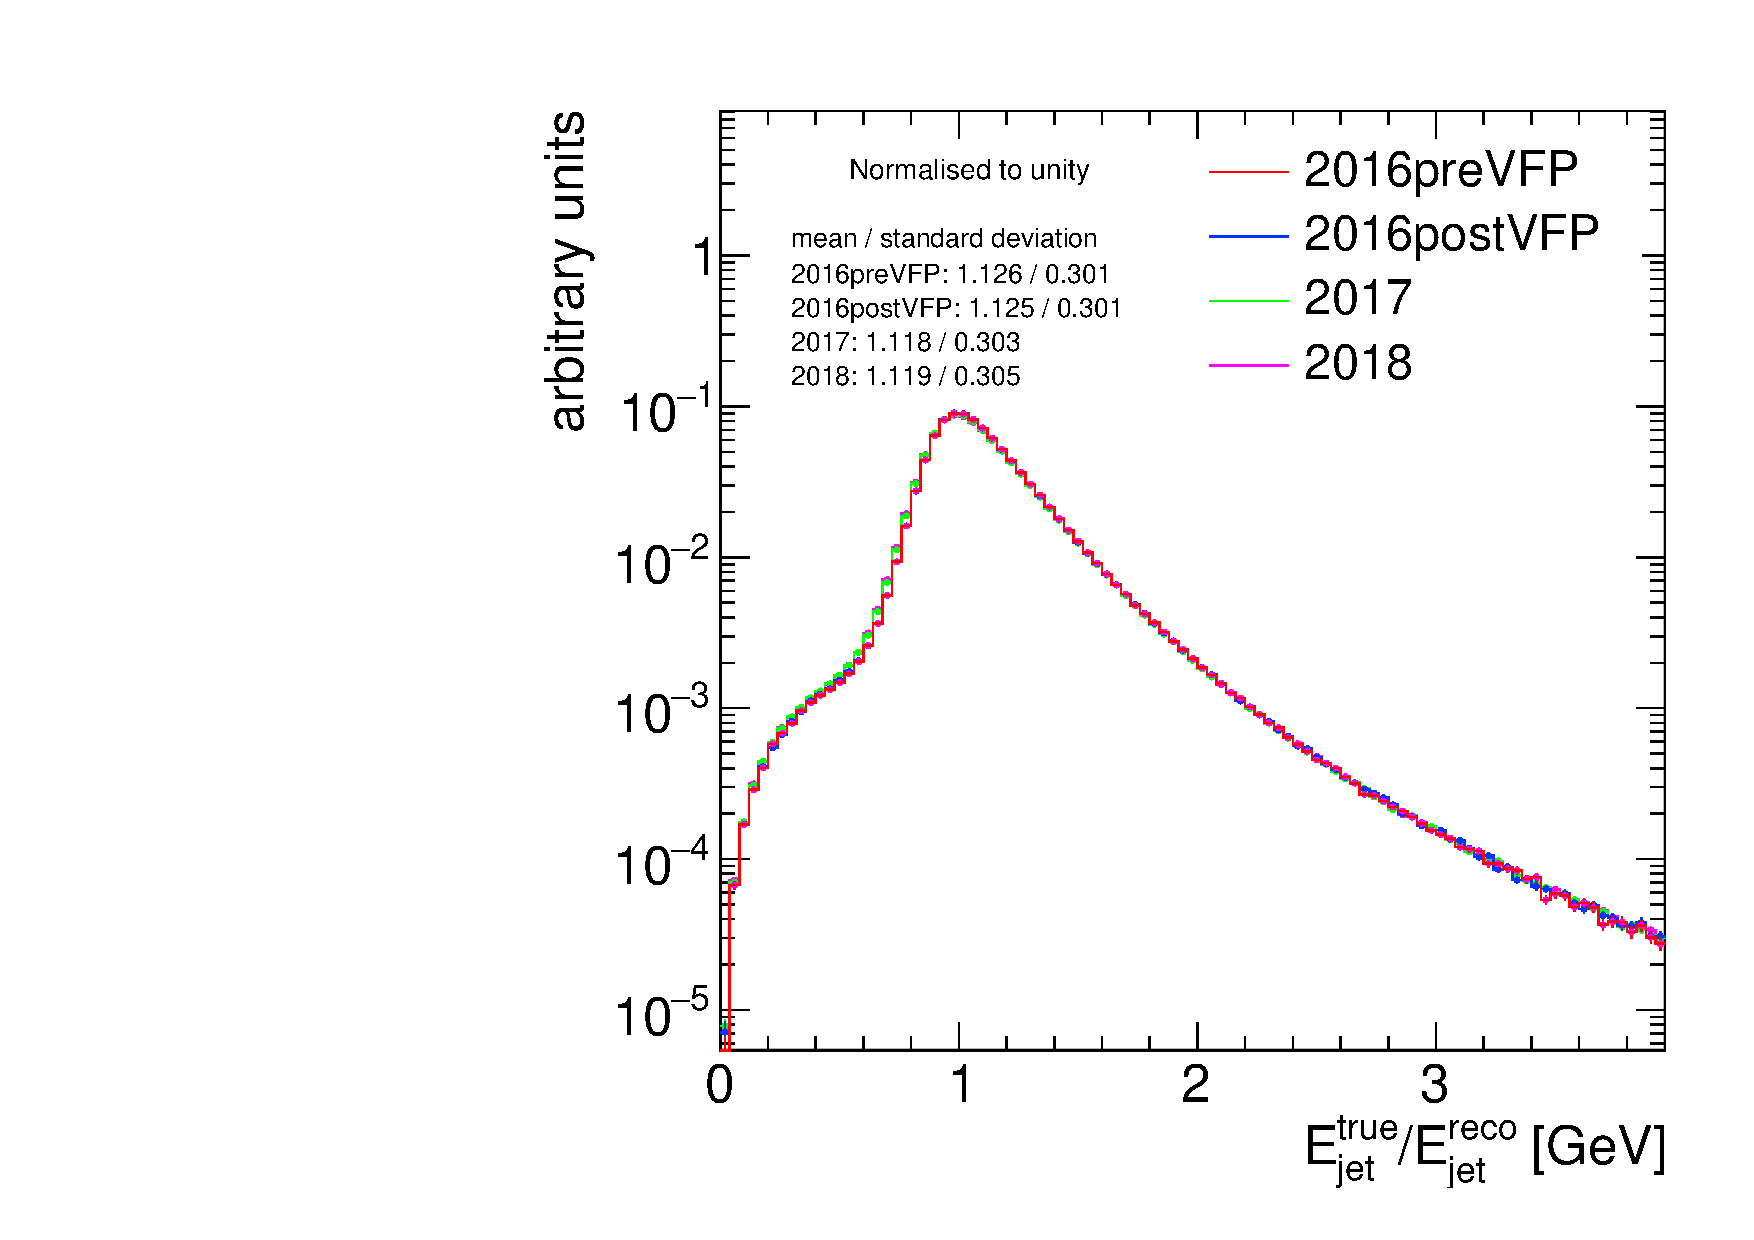
\includegraphics[width=0.30\textwidth]{fig_fullRun2UL/SmearingPlots/ULcomp_KinReco_fE_jet_step7.pdf}
        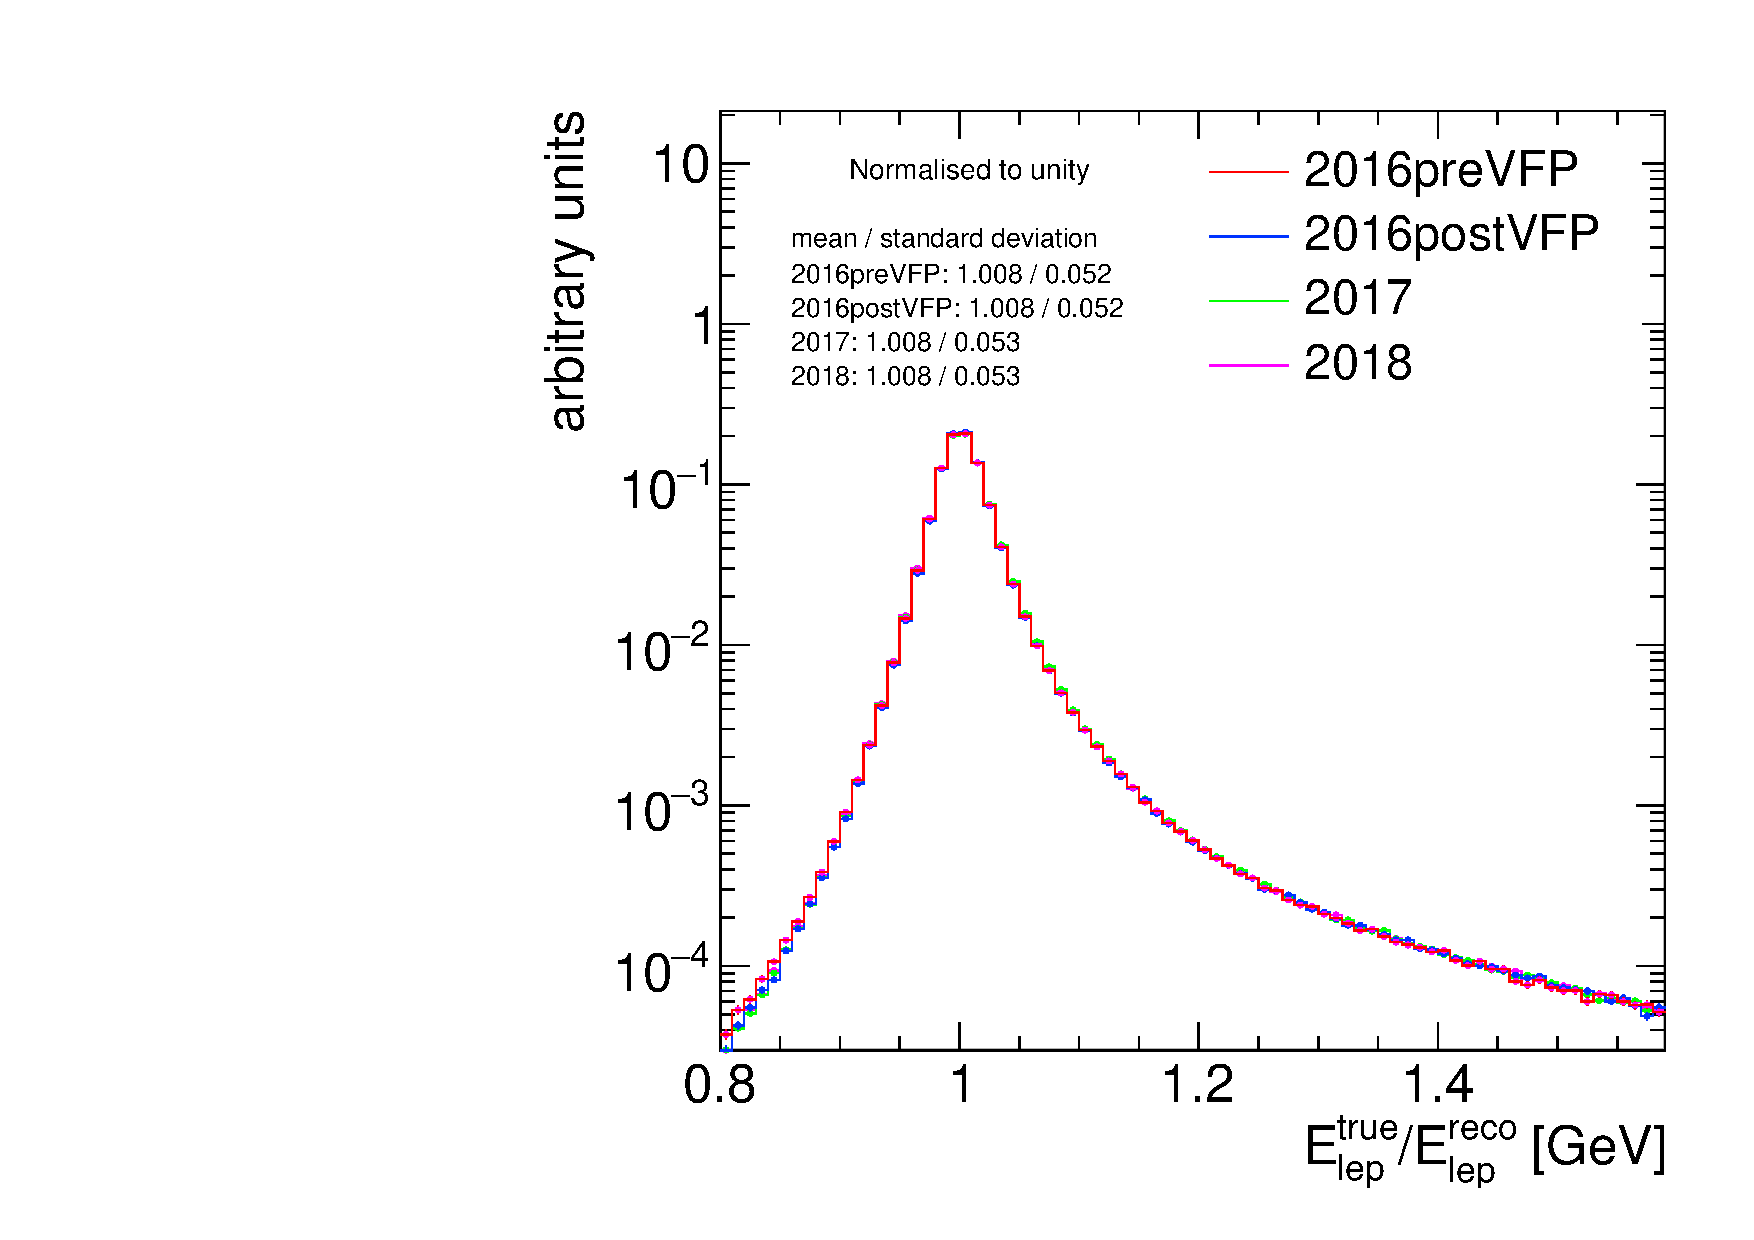
\includegraphics[width=0.30\textwidth]{fig_fullRun2UL/SmearingPlots/ULcomp_KinReco_fE_lep_step7.pdf}
        \caption{\small Distributions of the true energy divided by the reconstructed energy used for the energy smearing in the \ttbar full kinematic reconstruction. 
        The factors are shown for the b quarks (left) and the leptons (right).}
    \label{fig:energyFactor}
    \end{center}
\end{figure}

\begin{figure}[!htb]
    \begin{center}
        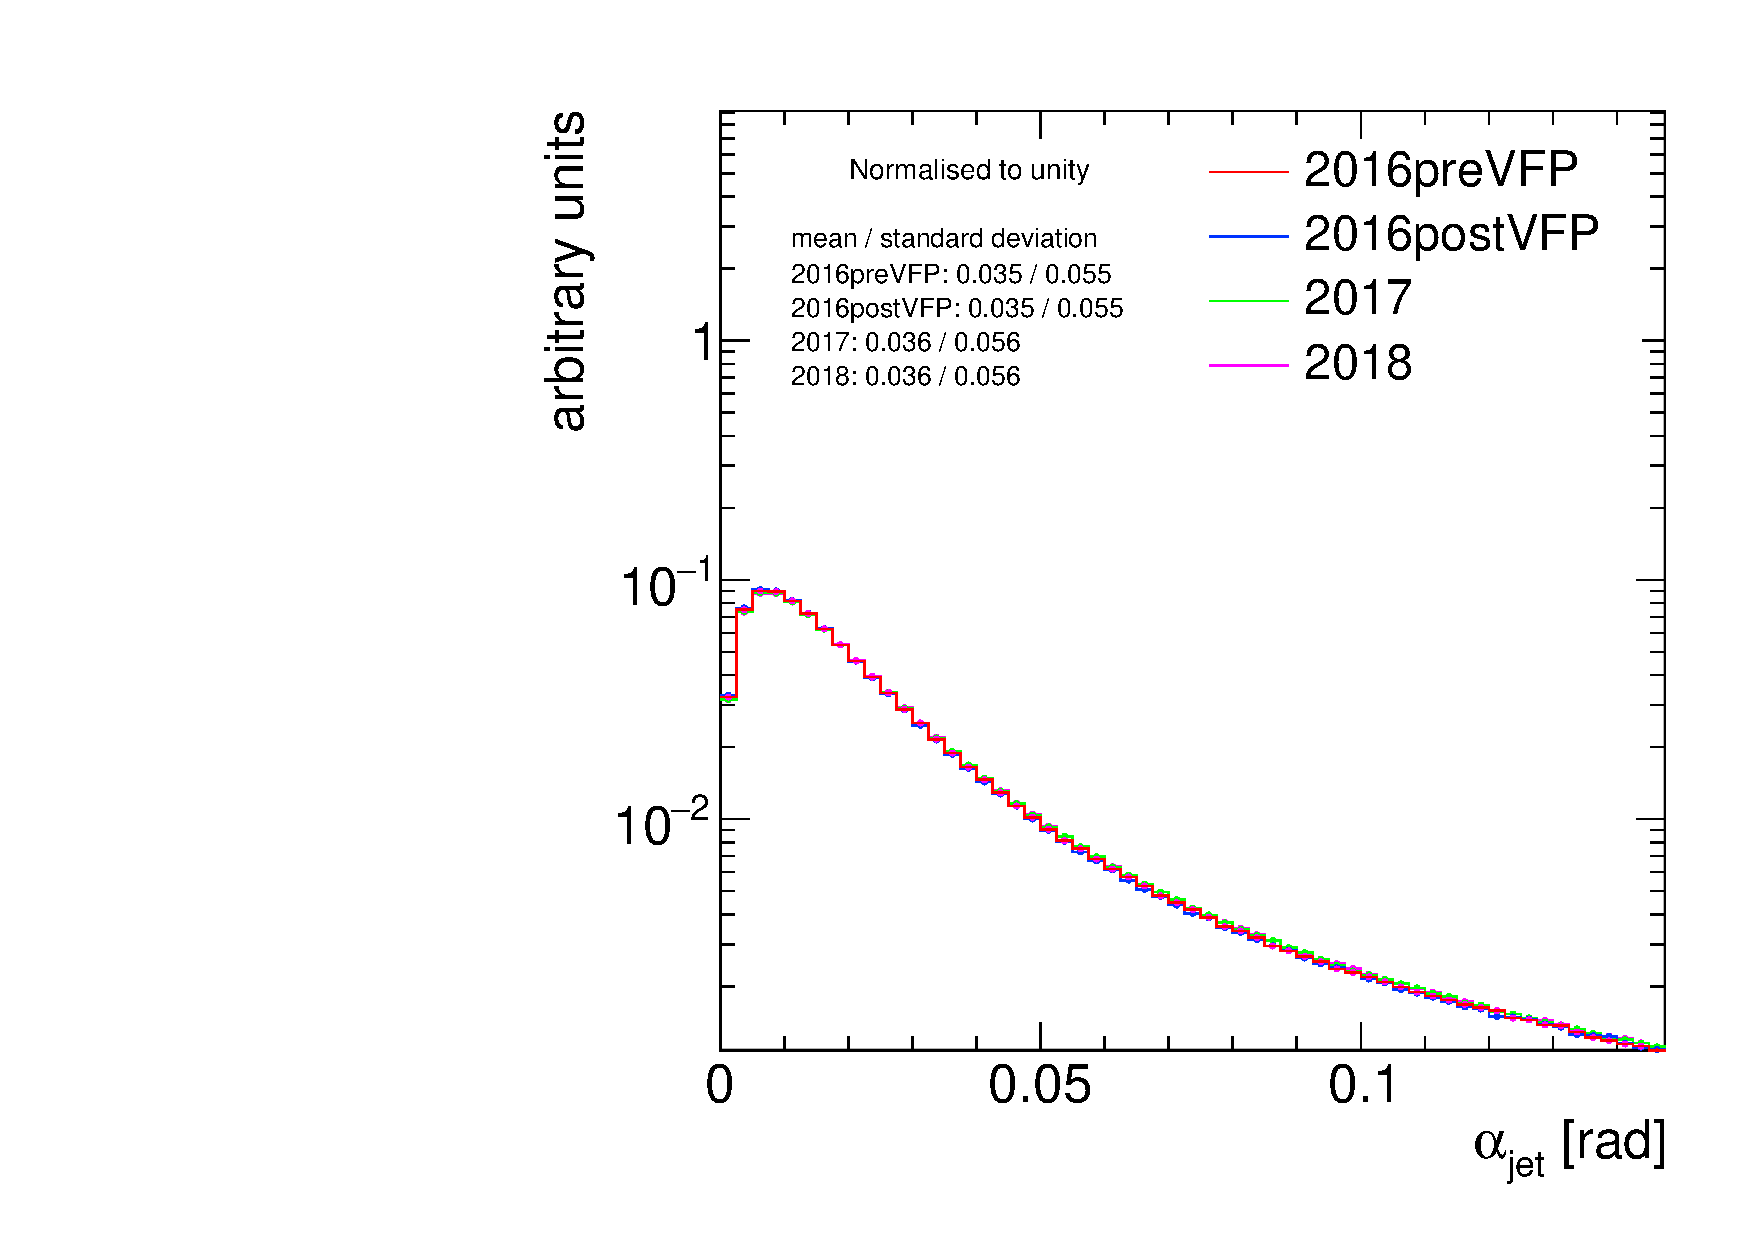
\includegraphics[width=0.30\textwidth]{fig_fullRun2UL/SmearingPlots/ULcomp_KinReco_d_angle_jet_step7.pdf}
        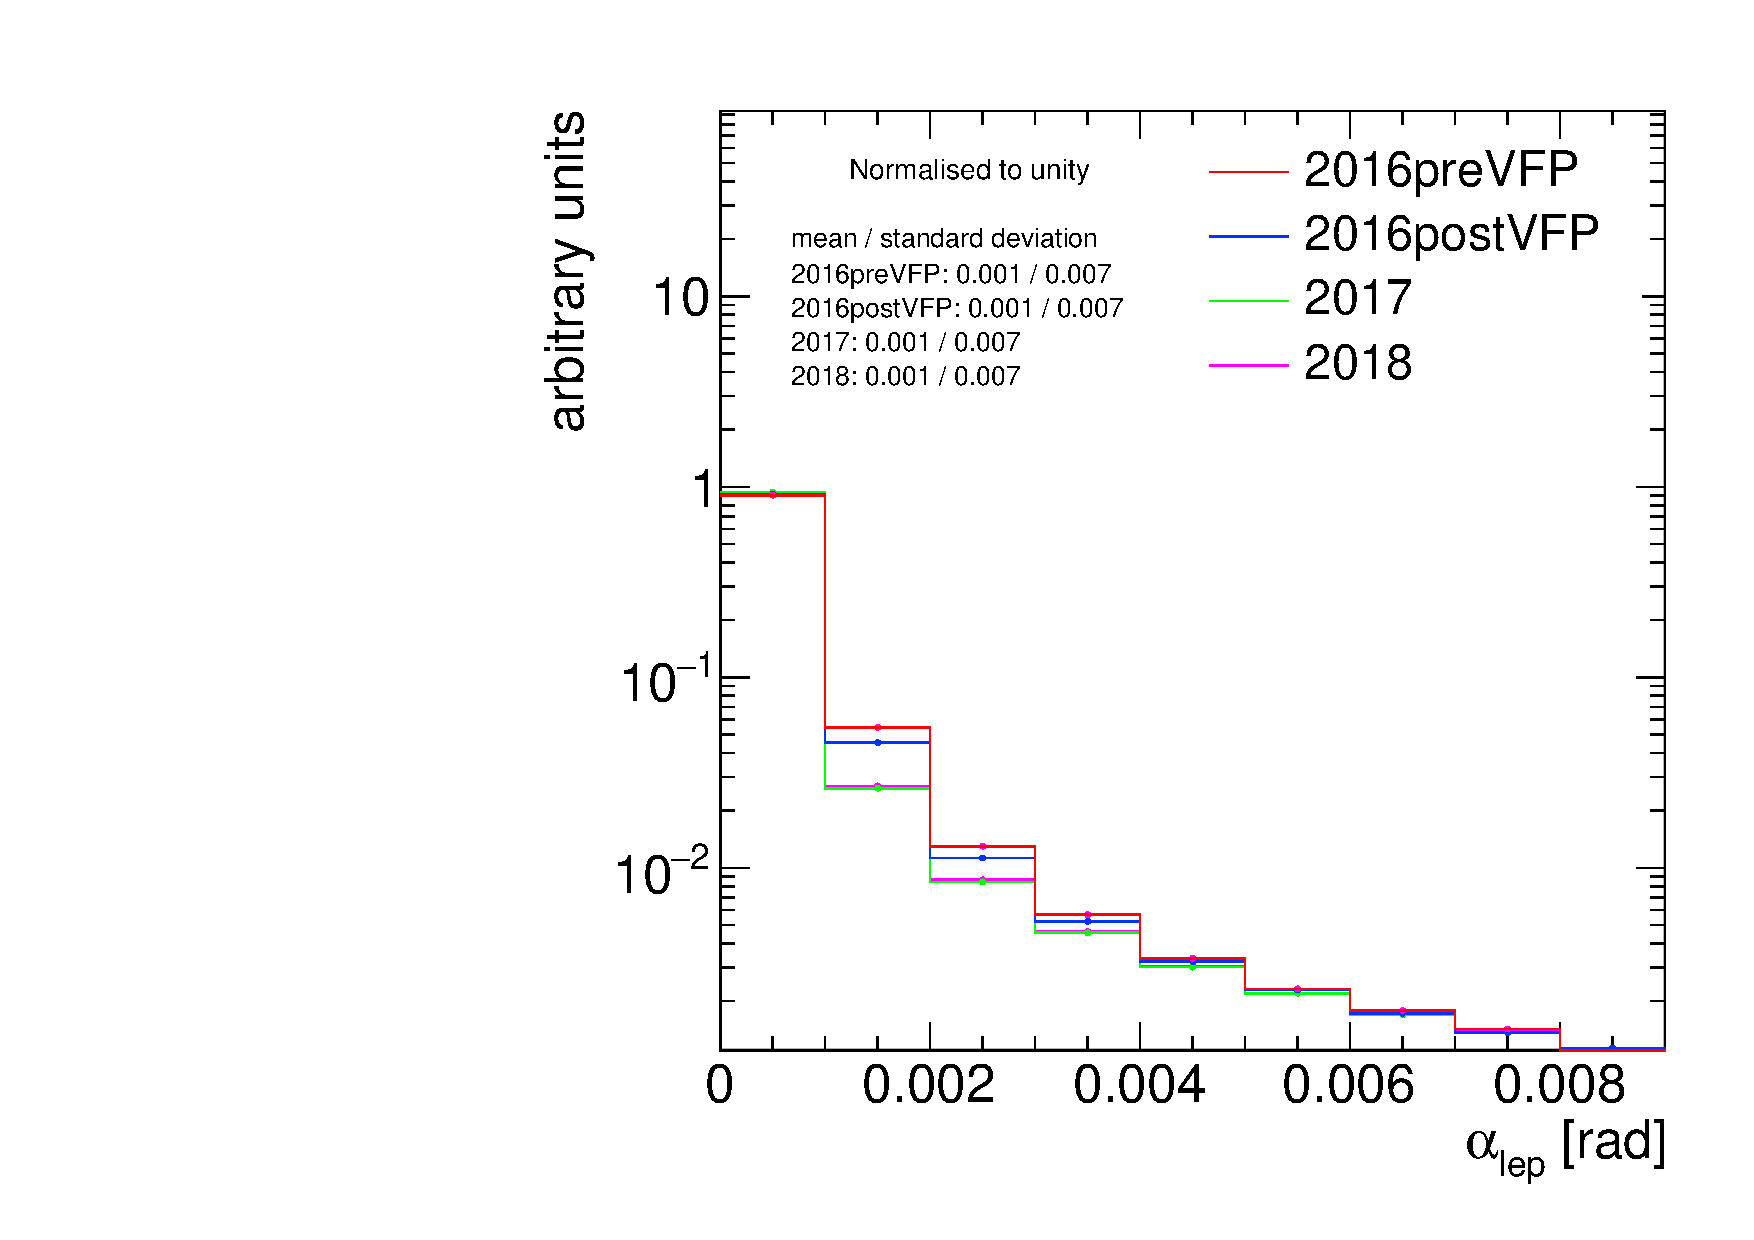
\includegraphics[width=0.30\textwidth]{fig_fullRun2UL/SmearingPlots/ULcomp_KinReco_d_angle_lep_step7.pdf}
        \caption{\small Distributions of the angle between the true direction and the reconstructed direction for jets (left) and leptons (right).}
       \label{fig:angleFactor}
    \end{center}
\end{figure}

\begin{figure}[!htb]
    \begin{center}
        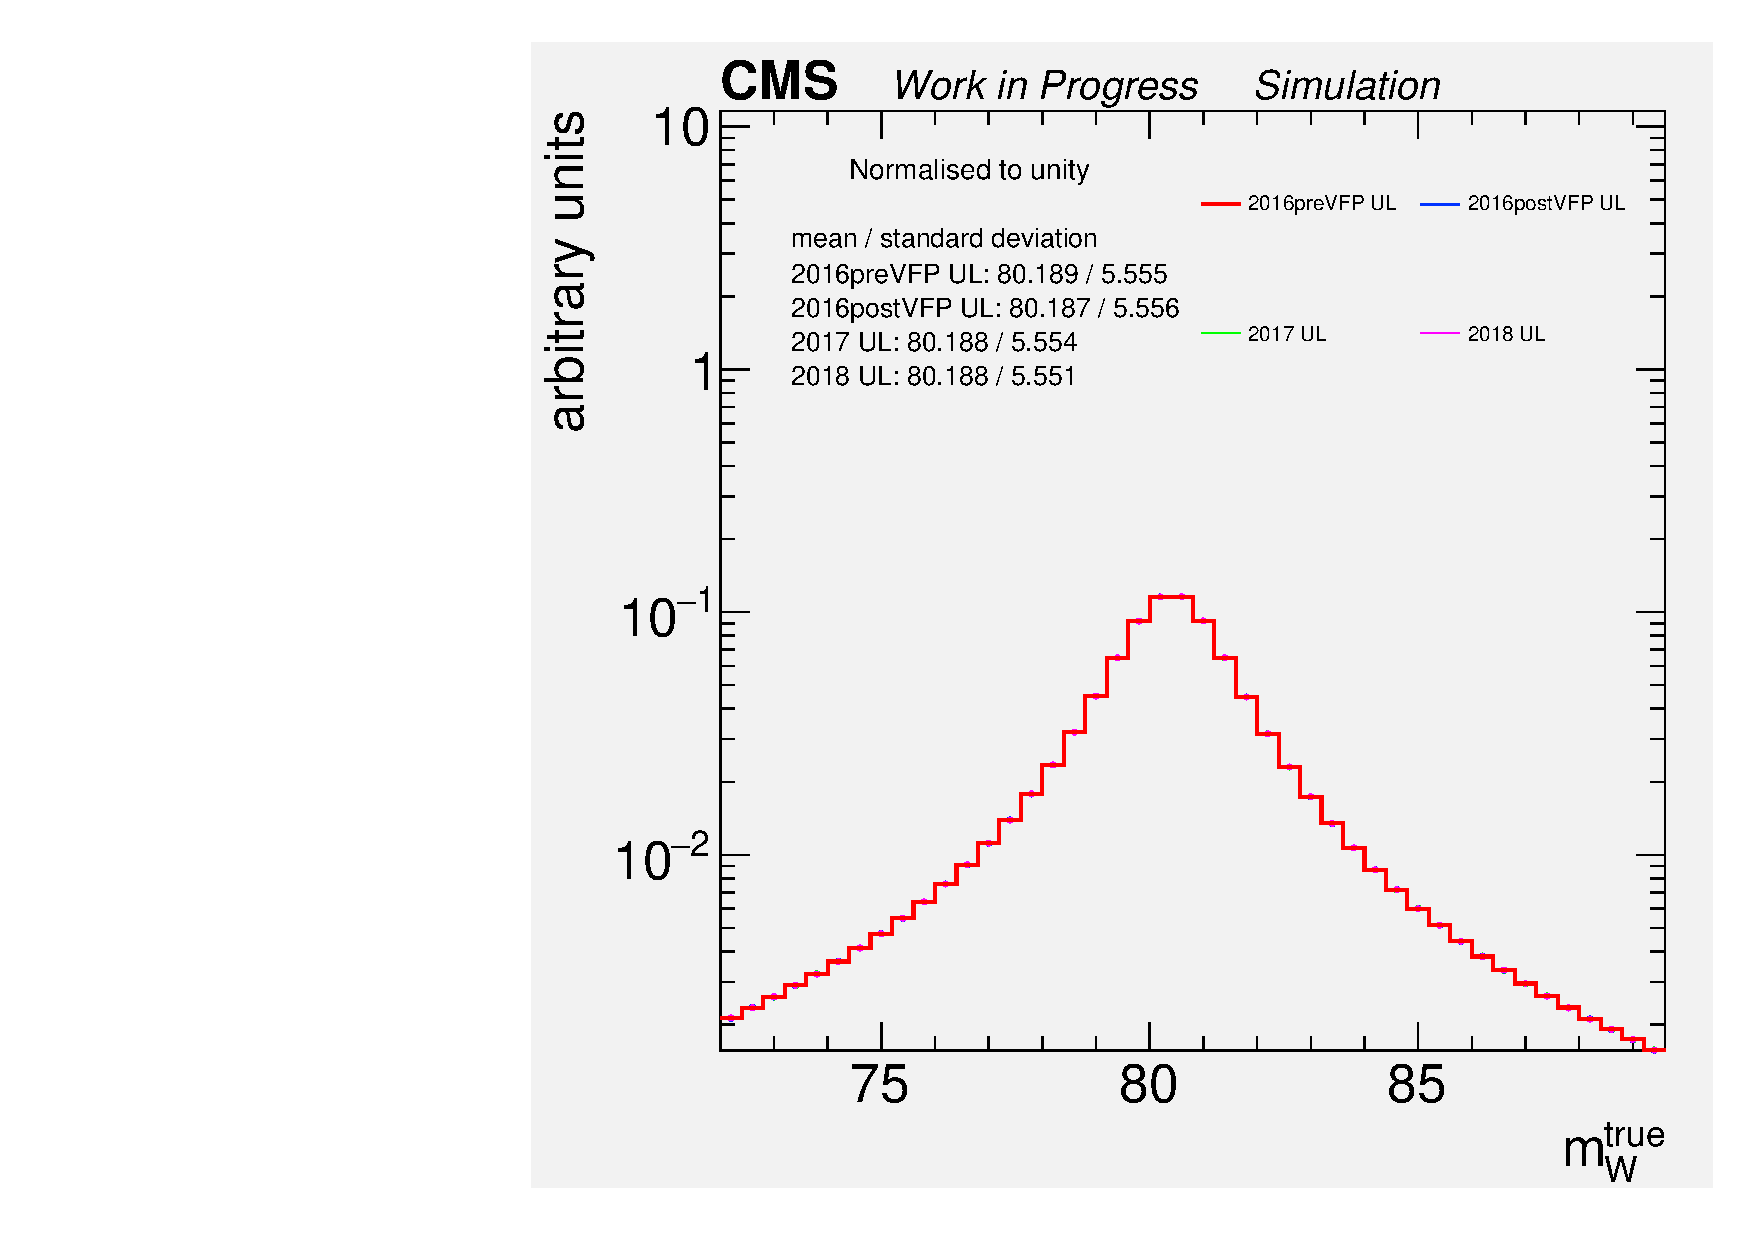
\includegraphics[width=0.30\textwidth]{fig_fullRun2UL/SmearingPlots/ULcomp_KinReco_W_mass_step0.pdf}
        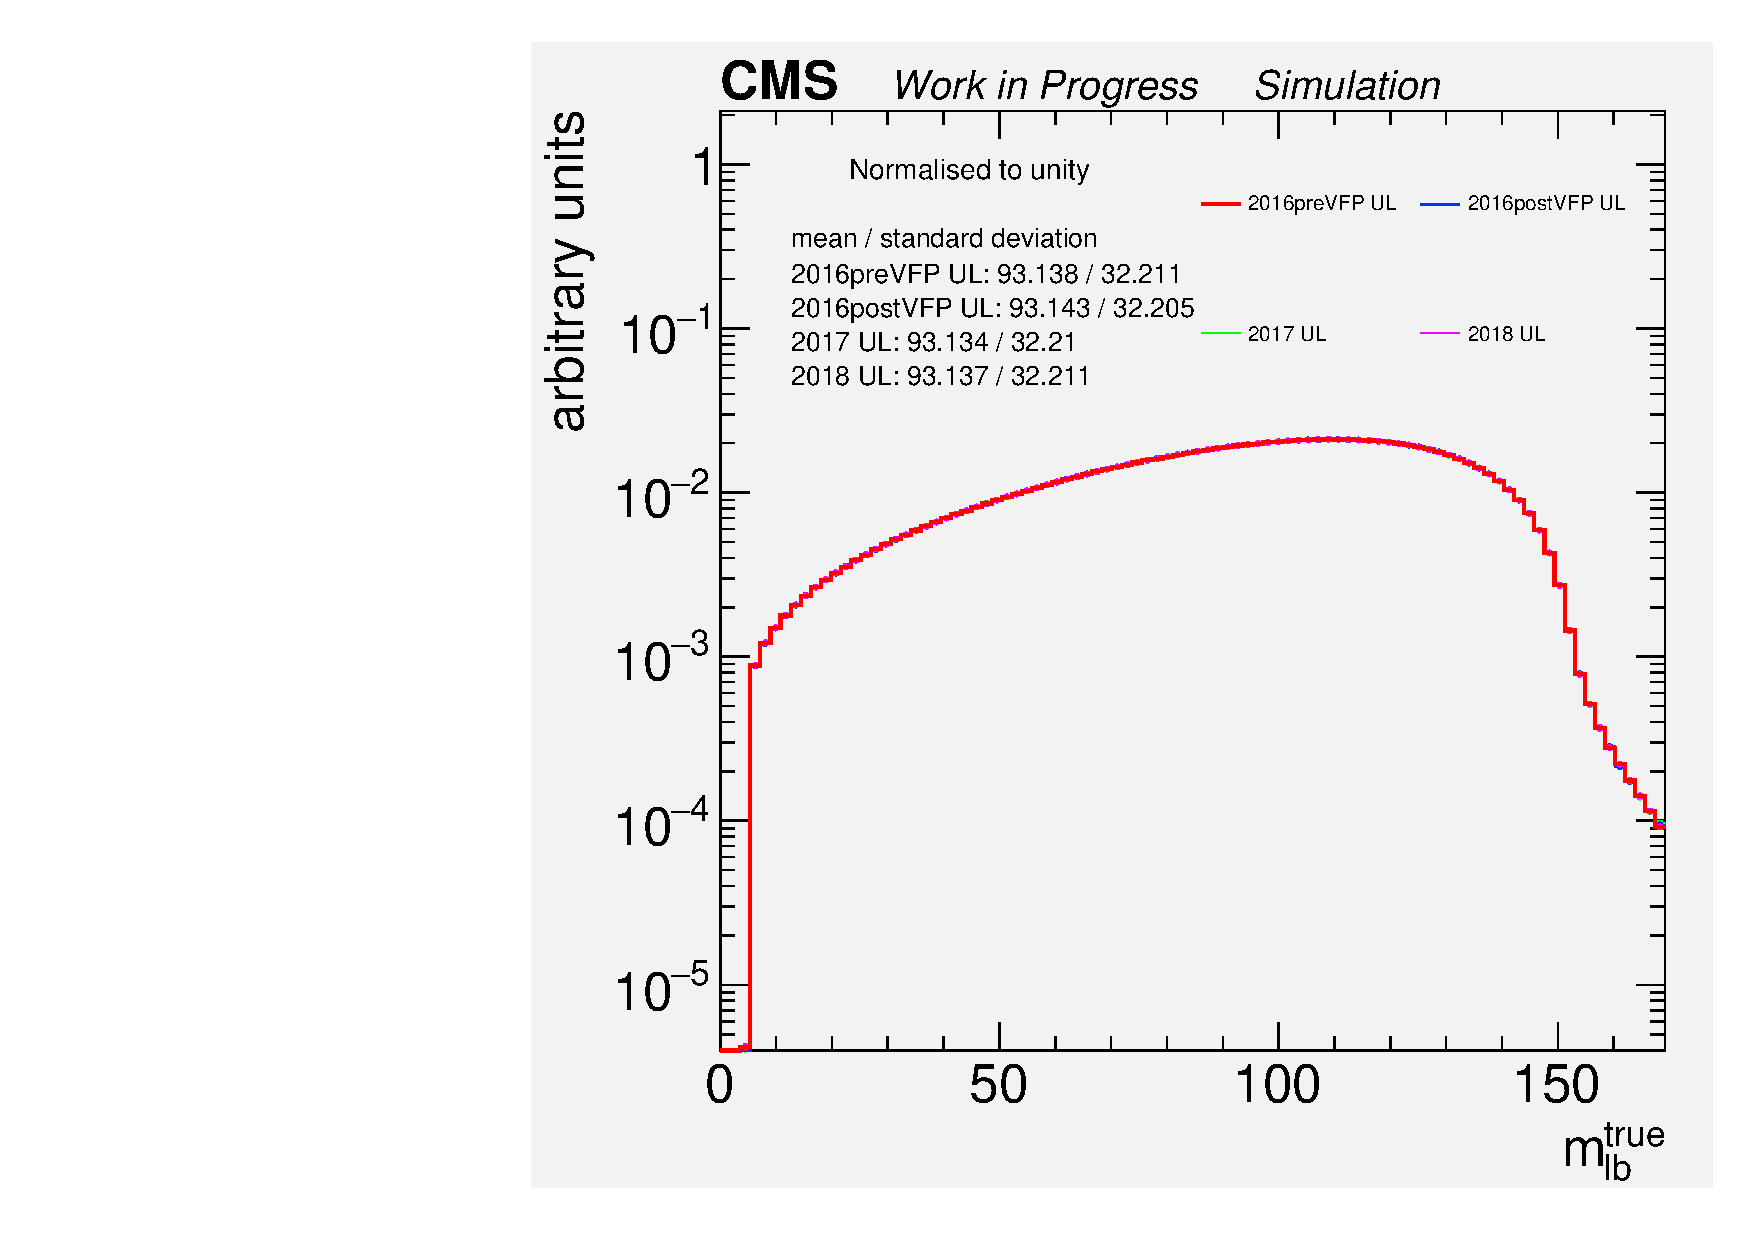
\includegraphics[width=0.30\textwidth]{fig_fullRun2UL/SmearingPlots/ULcomp_KinReco_mbl_true_step0.pdf}
        \caption{\small Distributions of the true W boson mass (left) and invariant mass distribution of reconstructed leptons and b-jets (right).}
       \label{fig:inputDists}
    \end{center}
\end{figure}

Likelihood weights for each smeared solution are calculated from the invariant mass of reconstructed leptons and b-jets relative to the true invariant mass distributions.
The true lepton-b-jet invariant mass distribution used to calculated solution likelihood weights is shown in figure~\ref{fig:inputDists}.
For each smearing, the jet--lepton assignments which yield the maximum weight are chosen.
A weighted average of all smeared solutions provides the final solution to the top quark three-momentum:
\begin{align}
\langle \vec{p}_{t} \rangle = \frac{1}{\mathcal{W}_s} \sum_{i=1}^{100} \mathcal{W}_i \cdot \vec{p}_{t,\,i} \quad \mbox{with} \quad \mathcal{W}_s = \sum_{i=1}^{100} \mathcal{W}_{i}
\end{align}
where $\mathcal{W}_i$ and $\vec{p}_{t,\,i}$ denote the weight and reconstructed top quark three-momentum obtained for the $i$-th smearing of the event.
Smearings without any solutions are given null weights.
The top quark energy is calculated from its three-momentum and the top quark mass constraint $m_{t} = \SI{172.5}{\GeV}$.
The final solution for top anti-quark four-momentum determined in an analogous procedure.

\subsection{Comparison of \ensuremath{\mathrm{t\bar{t}}} Reconstruction for Dilepton Events: Prompt and Via \ensuremath{\mathrm{\tau}}}
The assumption that the dilepton decay is prompt and there are only two neutrinos in the final state is not true when the dilepton decay is via intermediate $\tau$ leptons; such decays can have four or six neutrinos in the final state.
The top quark and \ttbar reconstructed kinematic variables at detector level (REC) are presented versus the true variables at generator level (GEN), and additionally the resolutions are presented as the difference between the true and reconstructed variables in bins of the true variables. 
Figures~\ref{fig:kinrec:resolution-mtt} through~\ref{fig:kinrec:resolution-yt} show resolution of \mtt, \ytt, \pttt, \yt, and \ptt\ distributions for both prompt and via tau reconstructed \ttbar dilepton events. 
The mean and sigma from a Gaussian fit to the kinematic variable resolutions are also included and reflect the bias and resolution of the algorithm, including degradation attributed to wrong jet--lepton assignments. 
We conclude that the resolution of \ttbar dilepton events via $\tau$ are comparable to prompt events, and thus are included as signal in this measurement.

\begin{figure}
  \begin{center}
    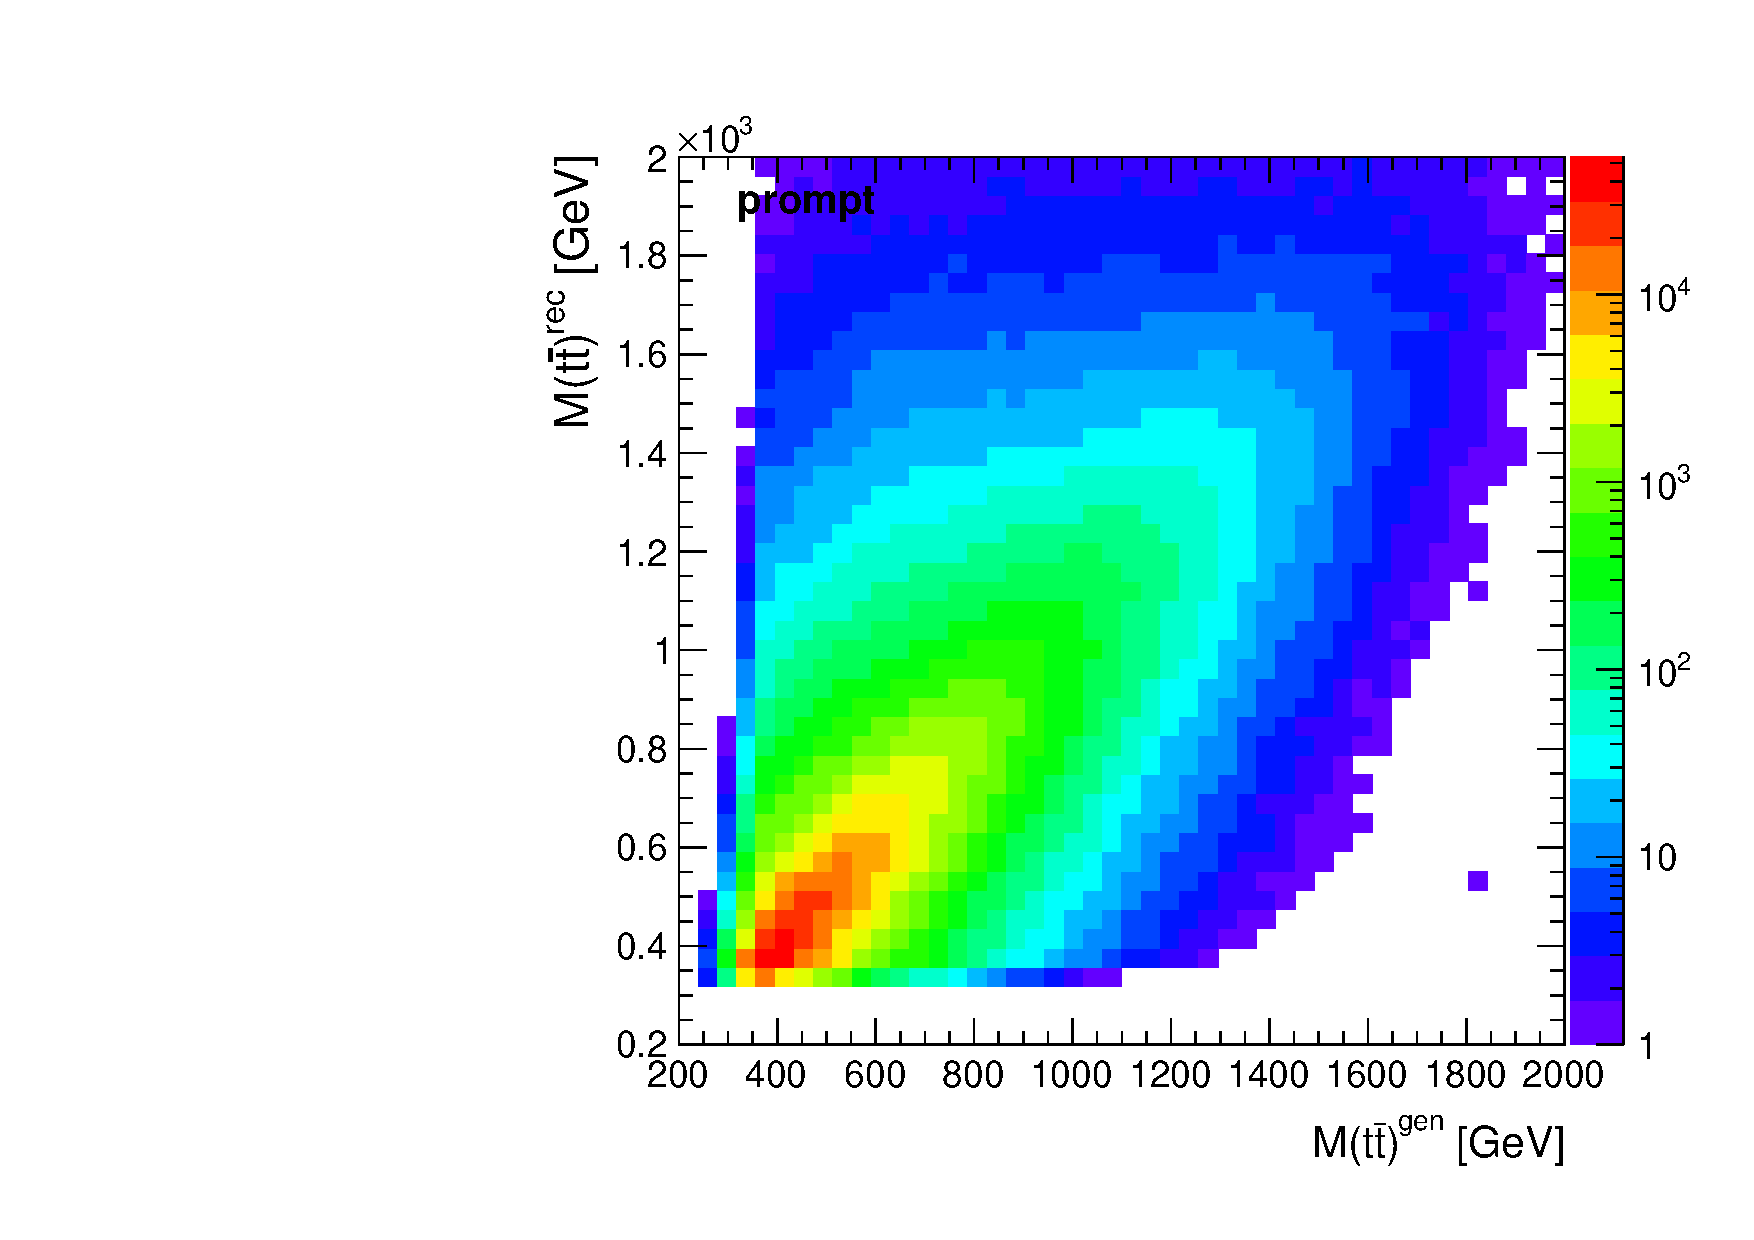
\includegraphics[width=0.30\textwidth]{fig_fullRun2UL/KinRecoResolutions/ttbar_mass_genreco_prompt.pdf}
    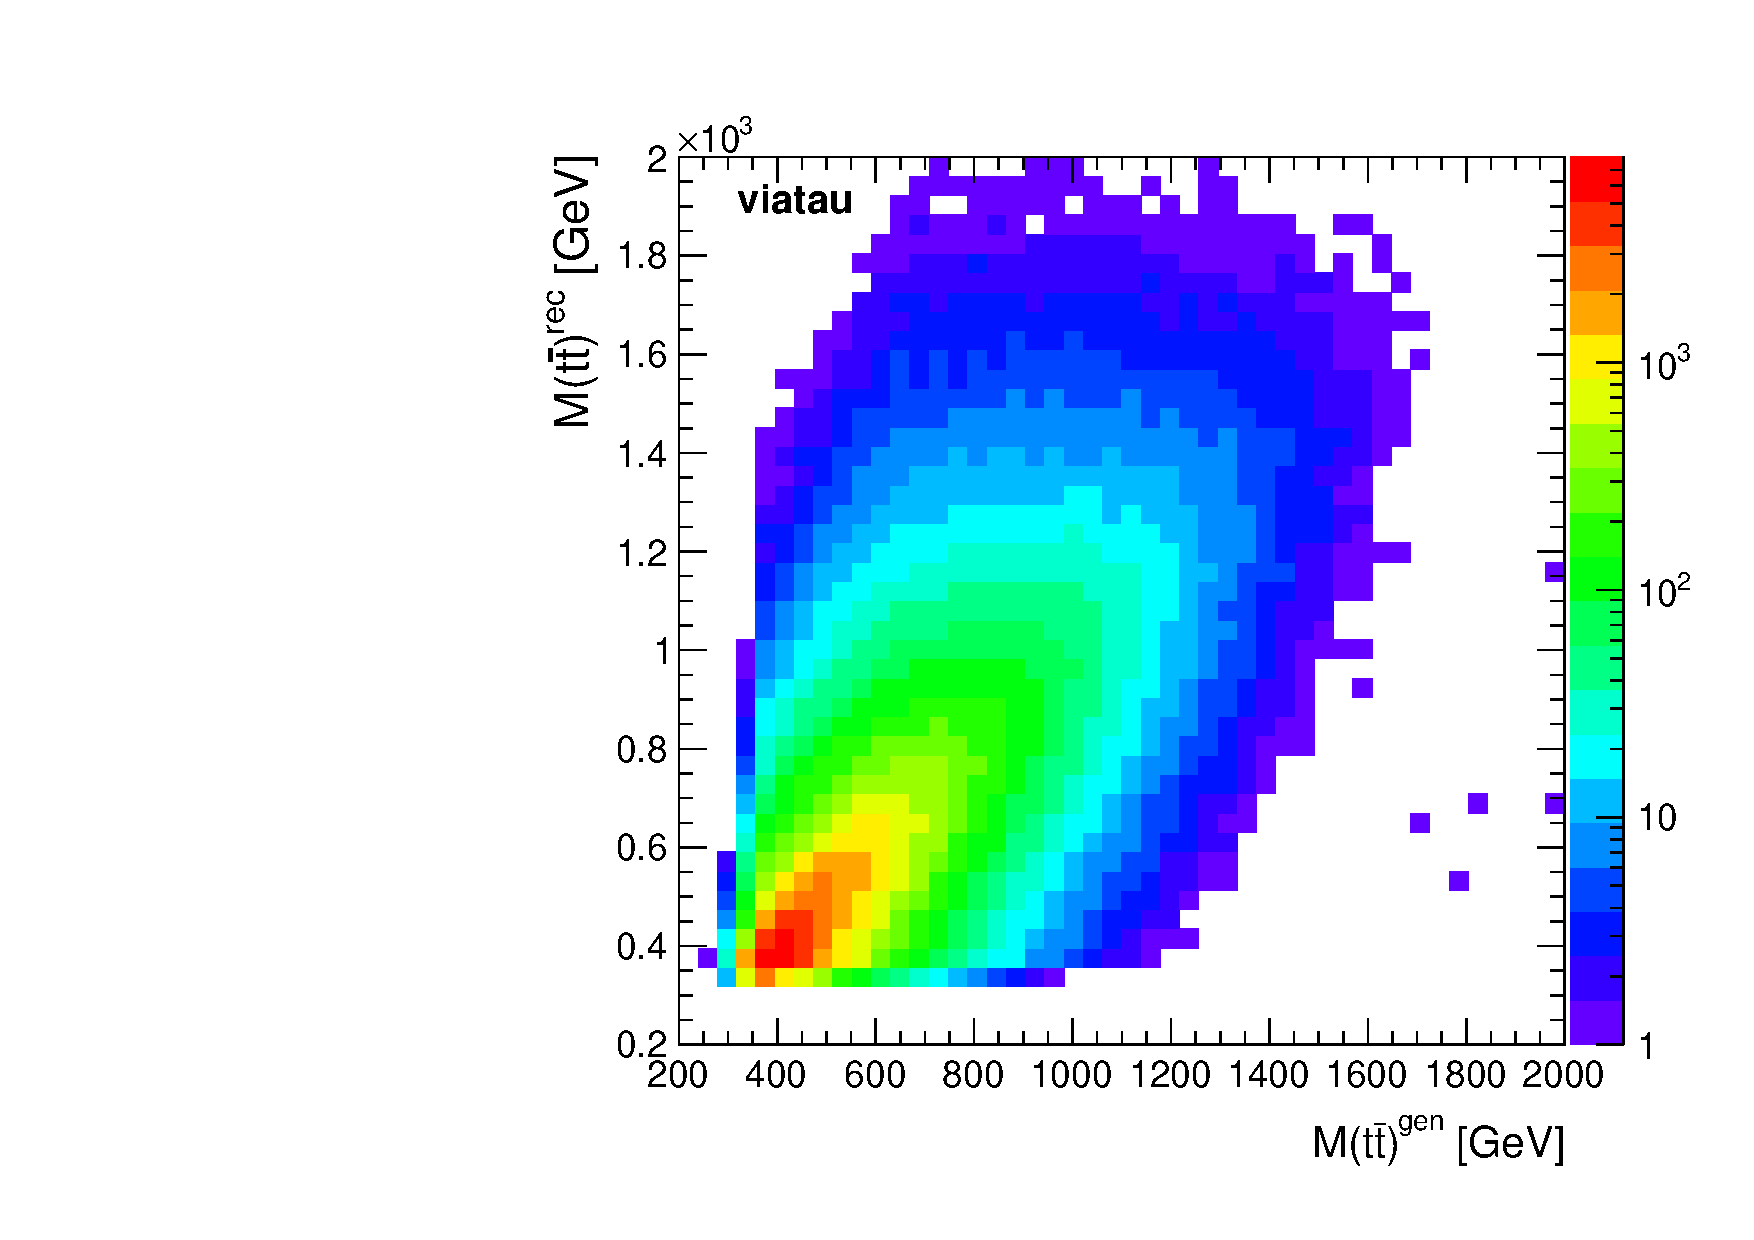
\includegraphics[width=0.30\textwidth]{fig_fullRun2UL/KinRecoResolutions/ttbar_mass_genreco_viatau.pdf}\\
    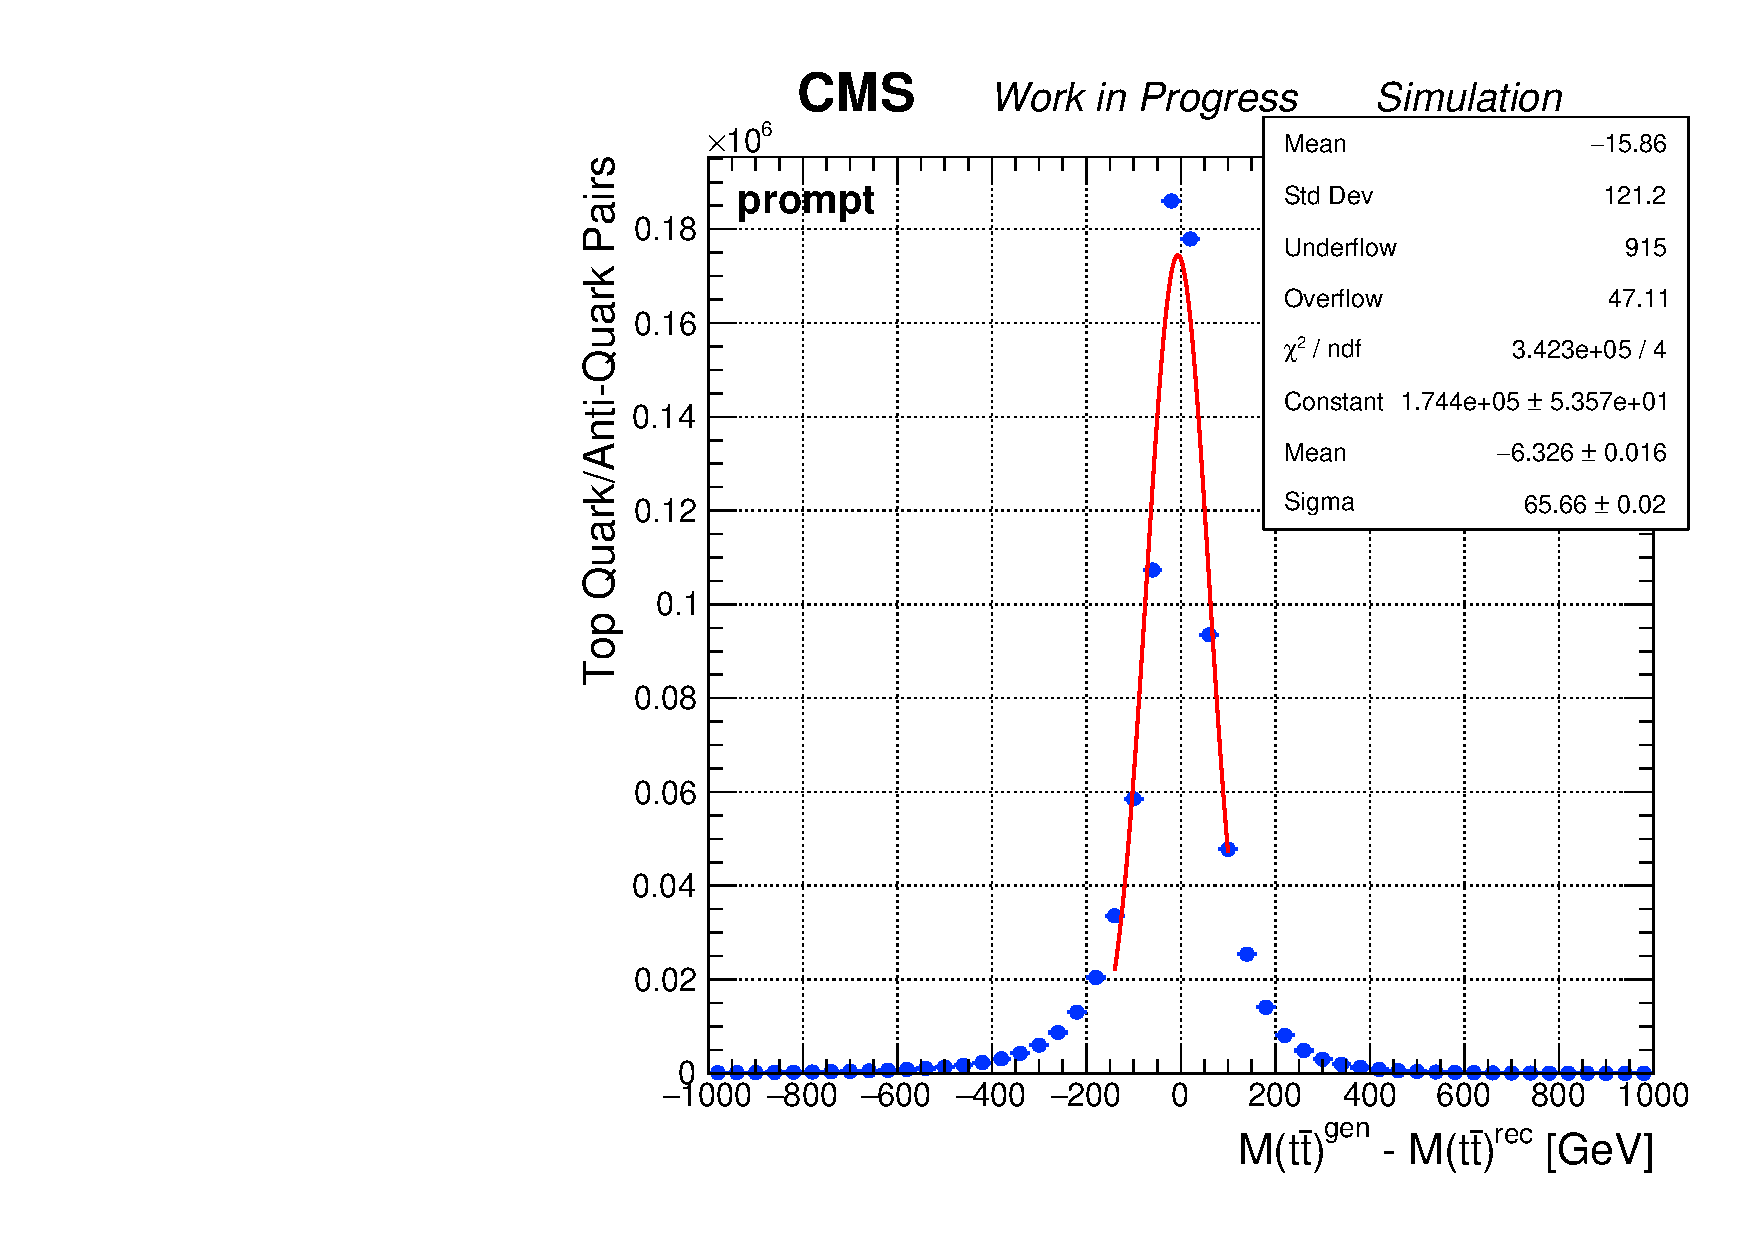
\includegraphics[width=0.30\textwidth]{fig_fullRun2UL/KinRecoResolutions/ttbar_mass_residual_prompt.pdf}
    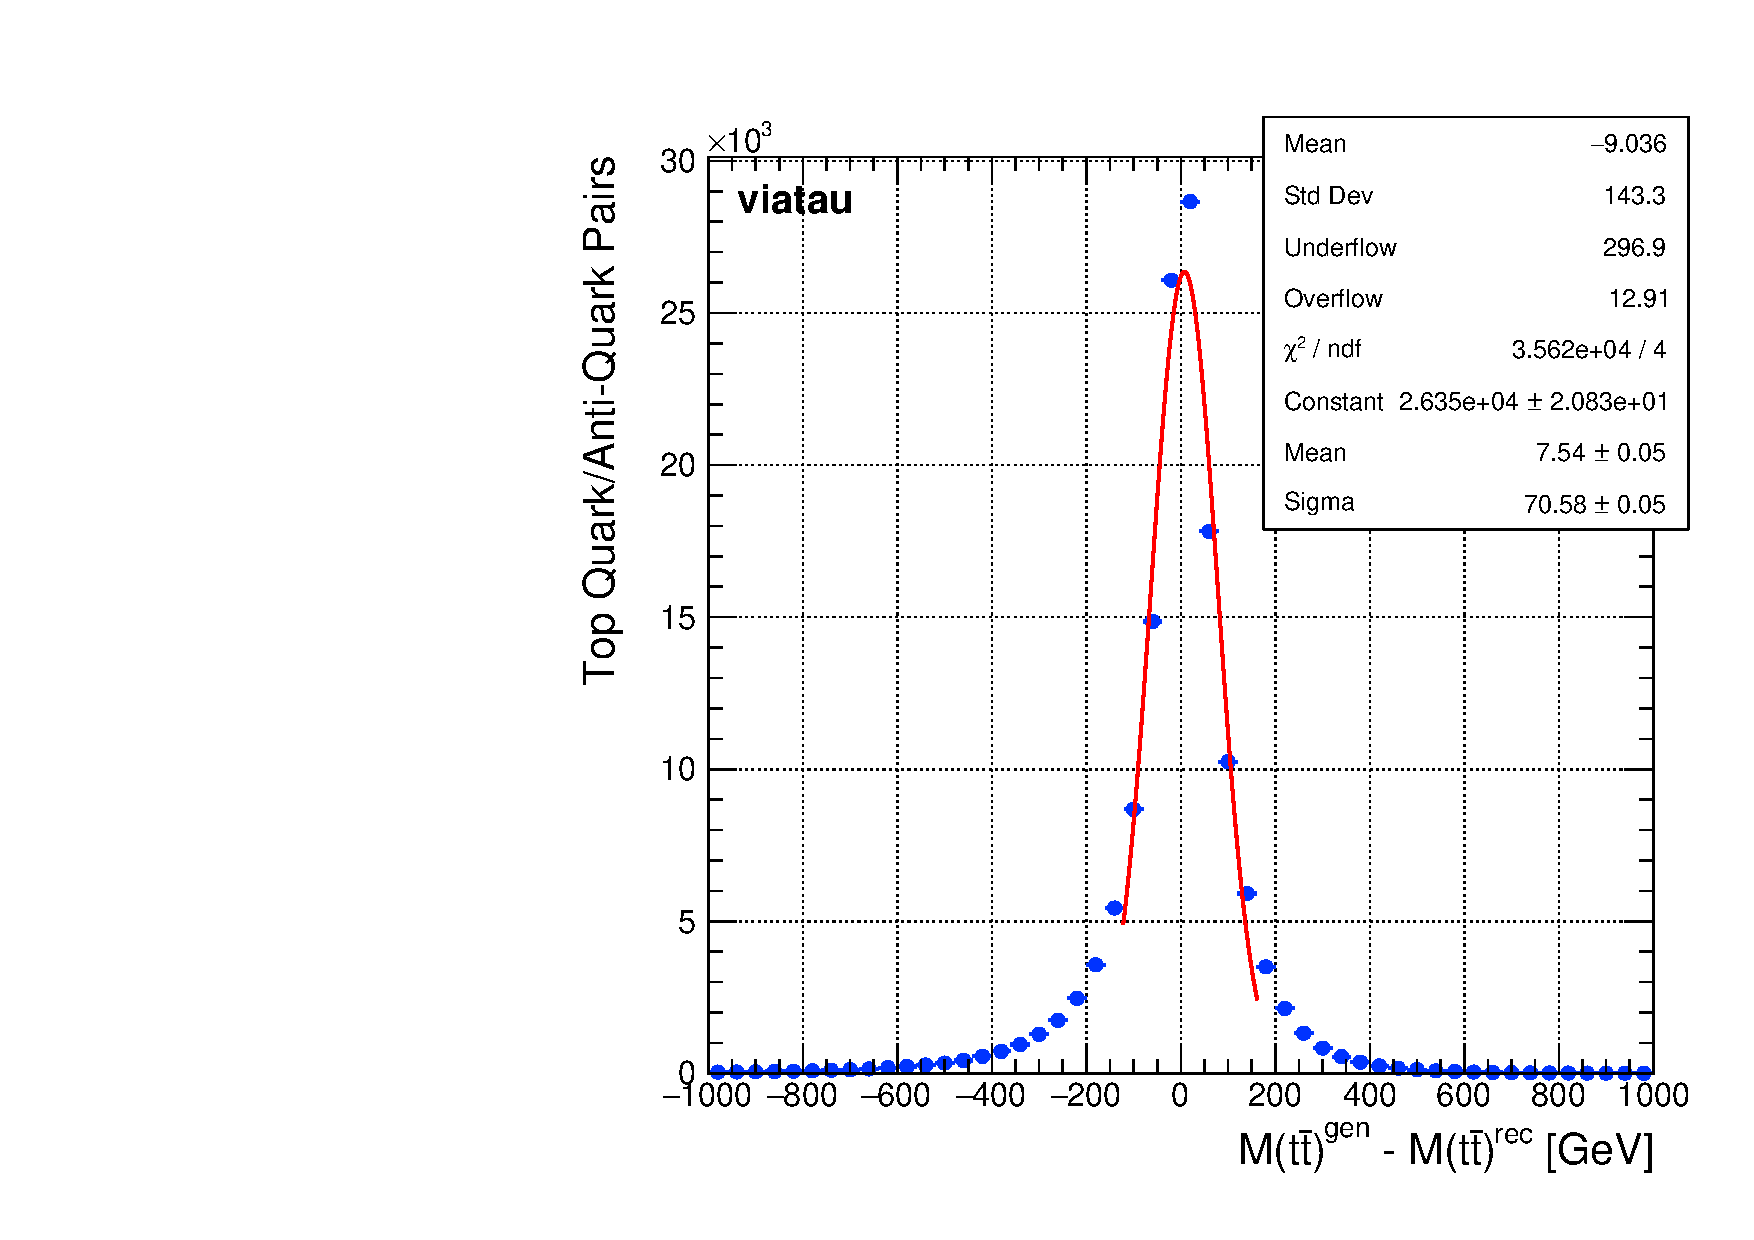
\includegraphics[width=0.30\textwidth]{fig_fullRun2UL/KinRecoResolutions/ttbar_mass_residual_viatau.pdf}\\
    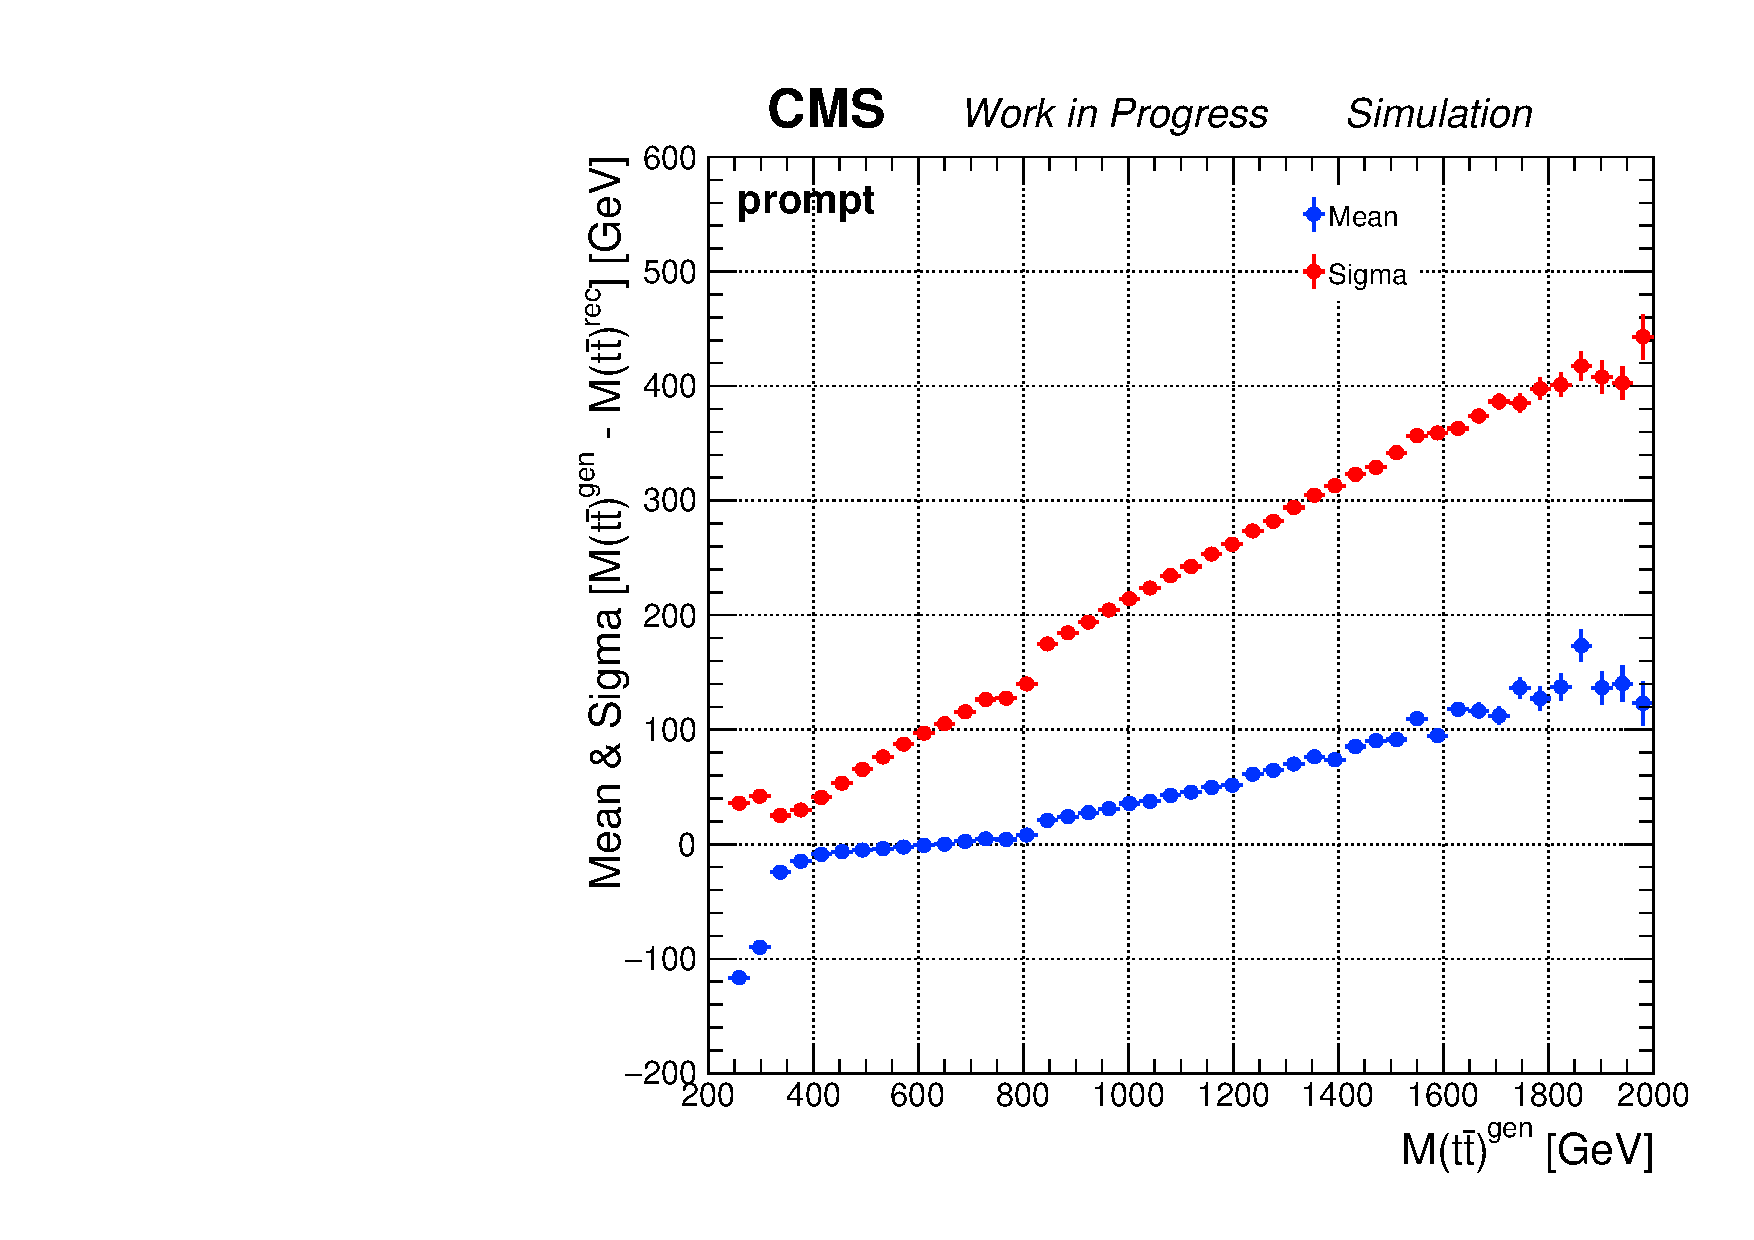
\includegraphics[width=0.30\textwidth]{fig_fullRun2UL/KinRecoResolutions/ttbar_mass_multiresidual_prompt.pdf}
    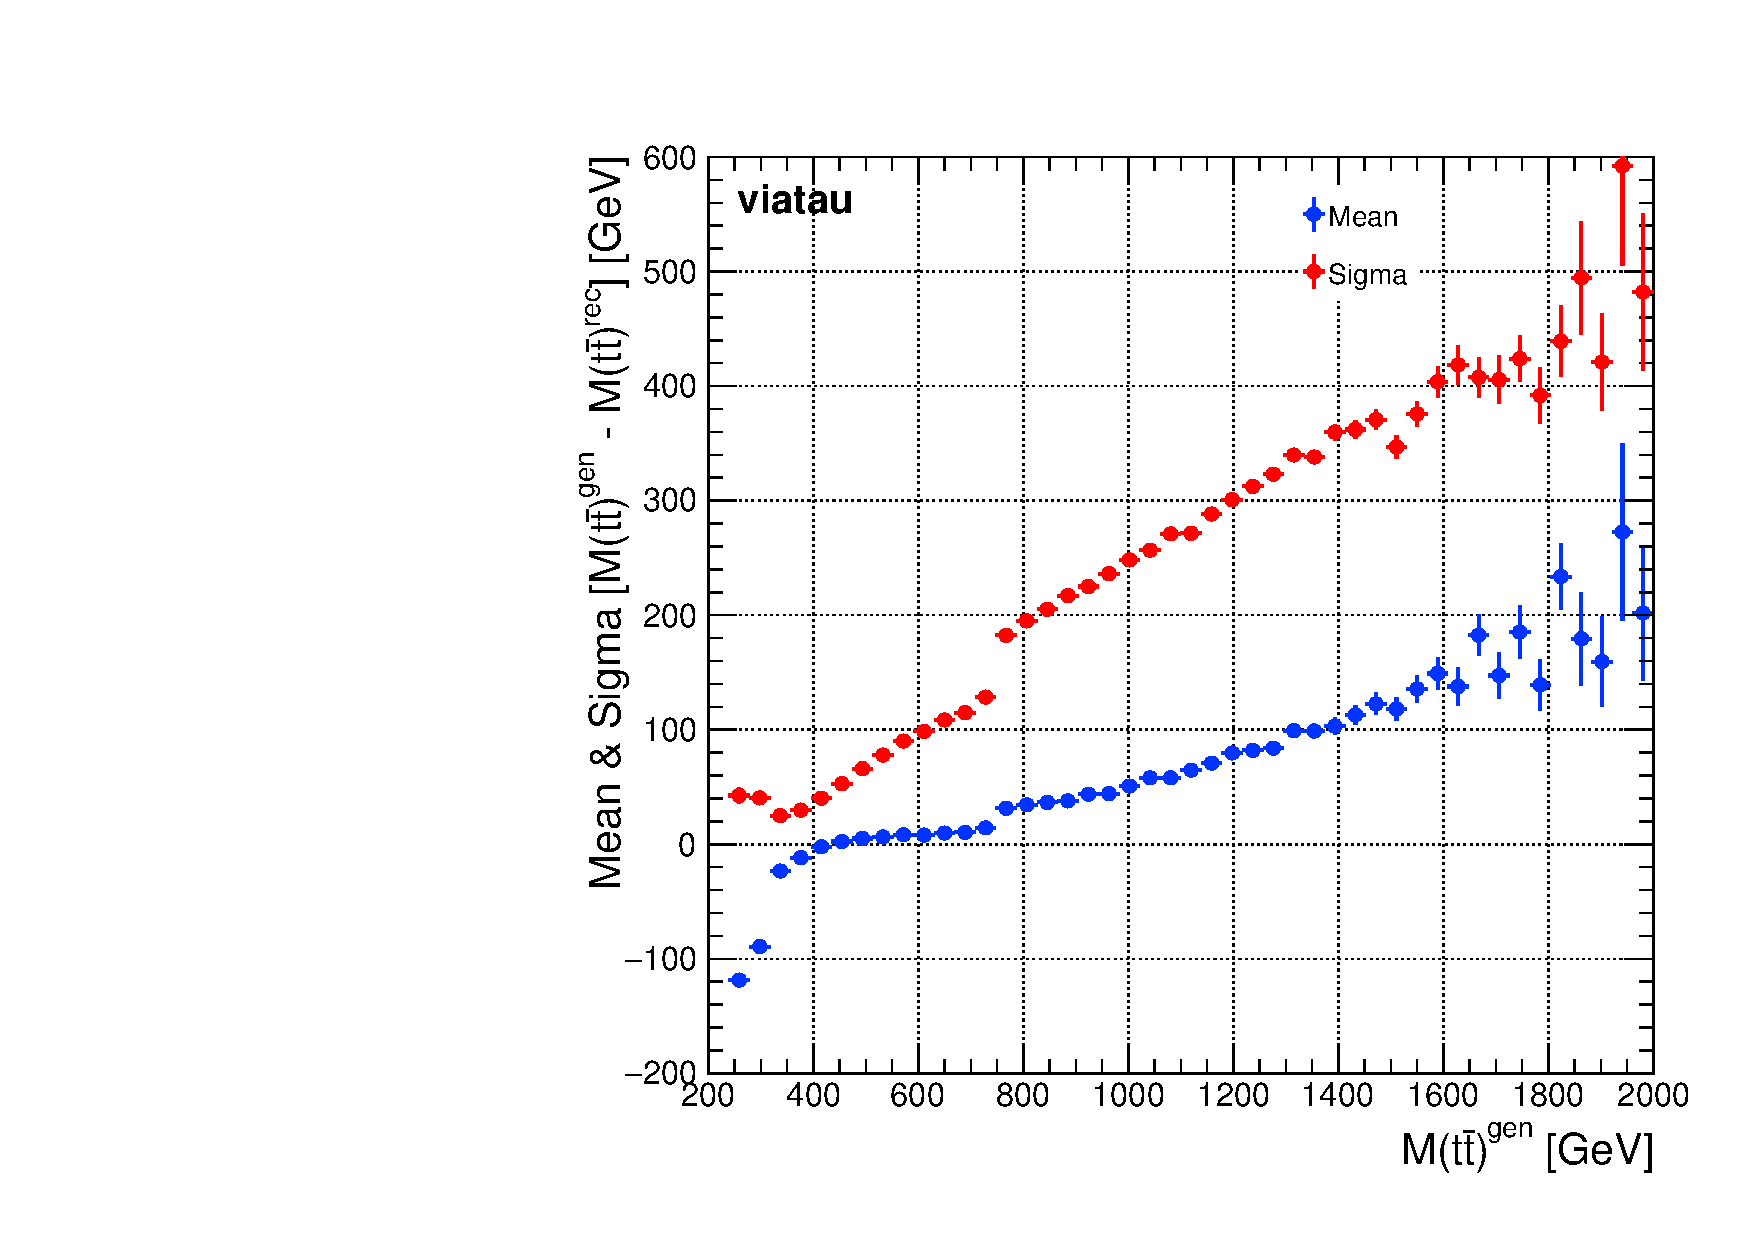
\includegraphics[width=0.30\textwidth]{fig_fullRun2UL/KinRecoResolutions/ttbar_mass_multiresidual_viatau.pdf}\\
    \caption{\small Top: True and reconstructed \mtt\ obtained for prompt (left) and via tau (right) \ttbar dilepton events.
    Middle: The difference between true and reconstructed \mtt\ in bins of true \mtt\ (fitted with a Gaussian function for illustration).
    Bottom: The differential mean and sigma from Gaussian fits, with respect to true \mtt, of the difference between true and reconstructed \mtt\ obtained for prompt and via tau \ttbar dilepton events.
    The simulated samples are normalized to an integrated luminosity of \lumivalueRuniiUL.}
    \label{fig:kinrec:resolution-mtt}
 \end{center}
\end{figure}

\begin{figure}
  \begin{center}
    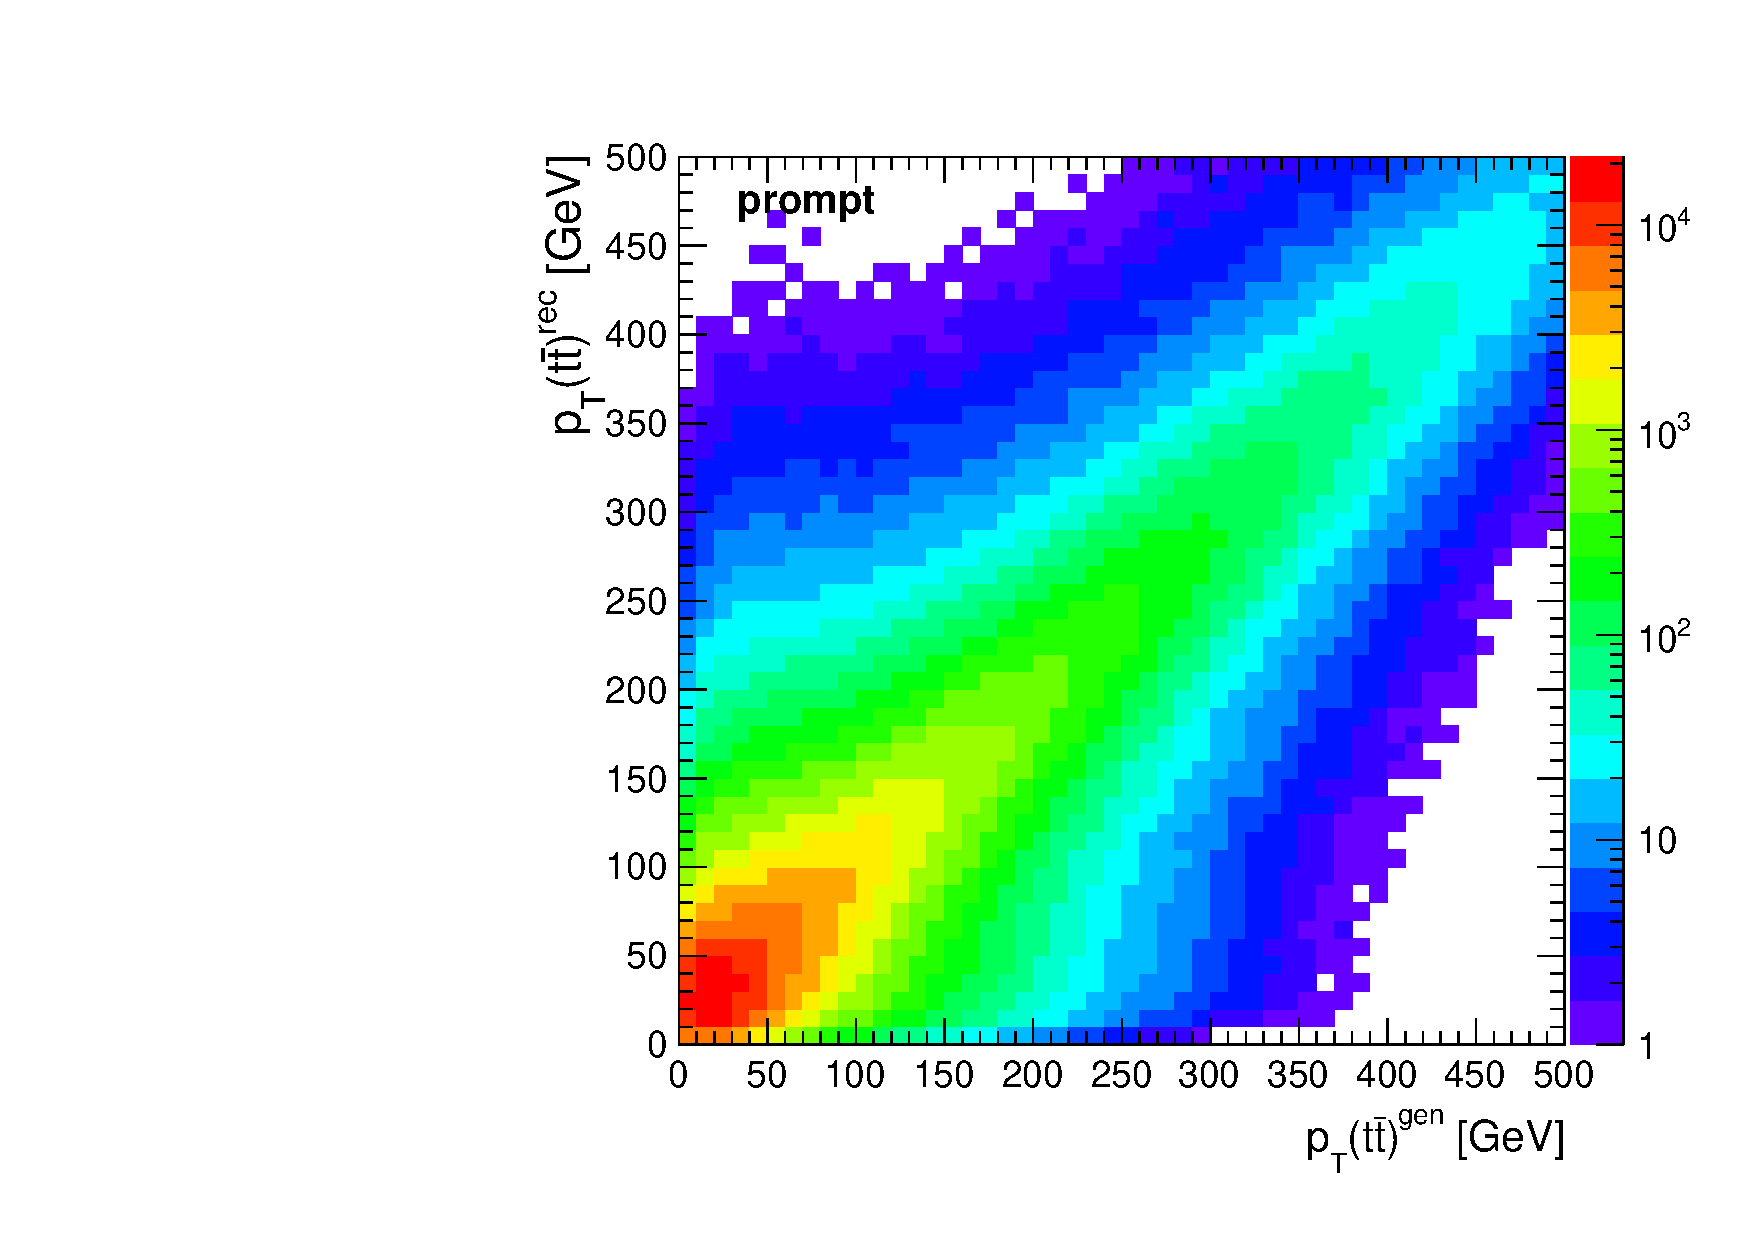
\includegraphics[width=0.30\textwidth]{fig_fullRun2UL/KinRecoResolutions/ttbar_pT_genreco_prompt.pdf}
    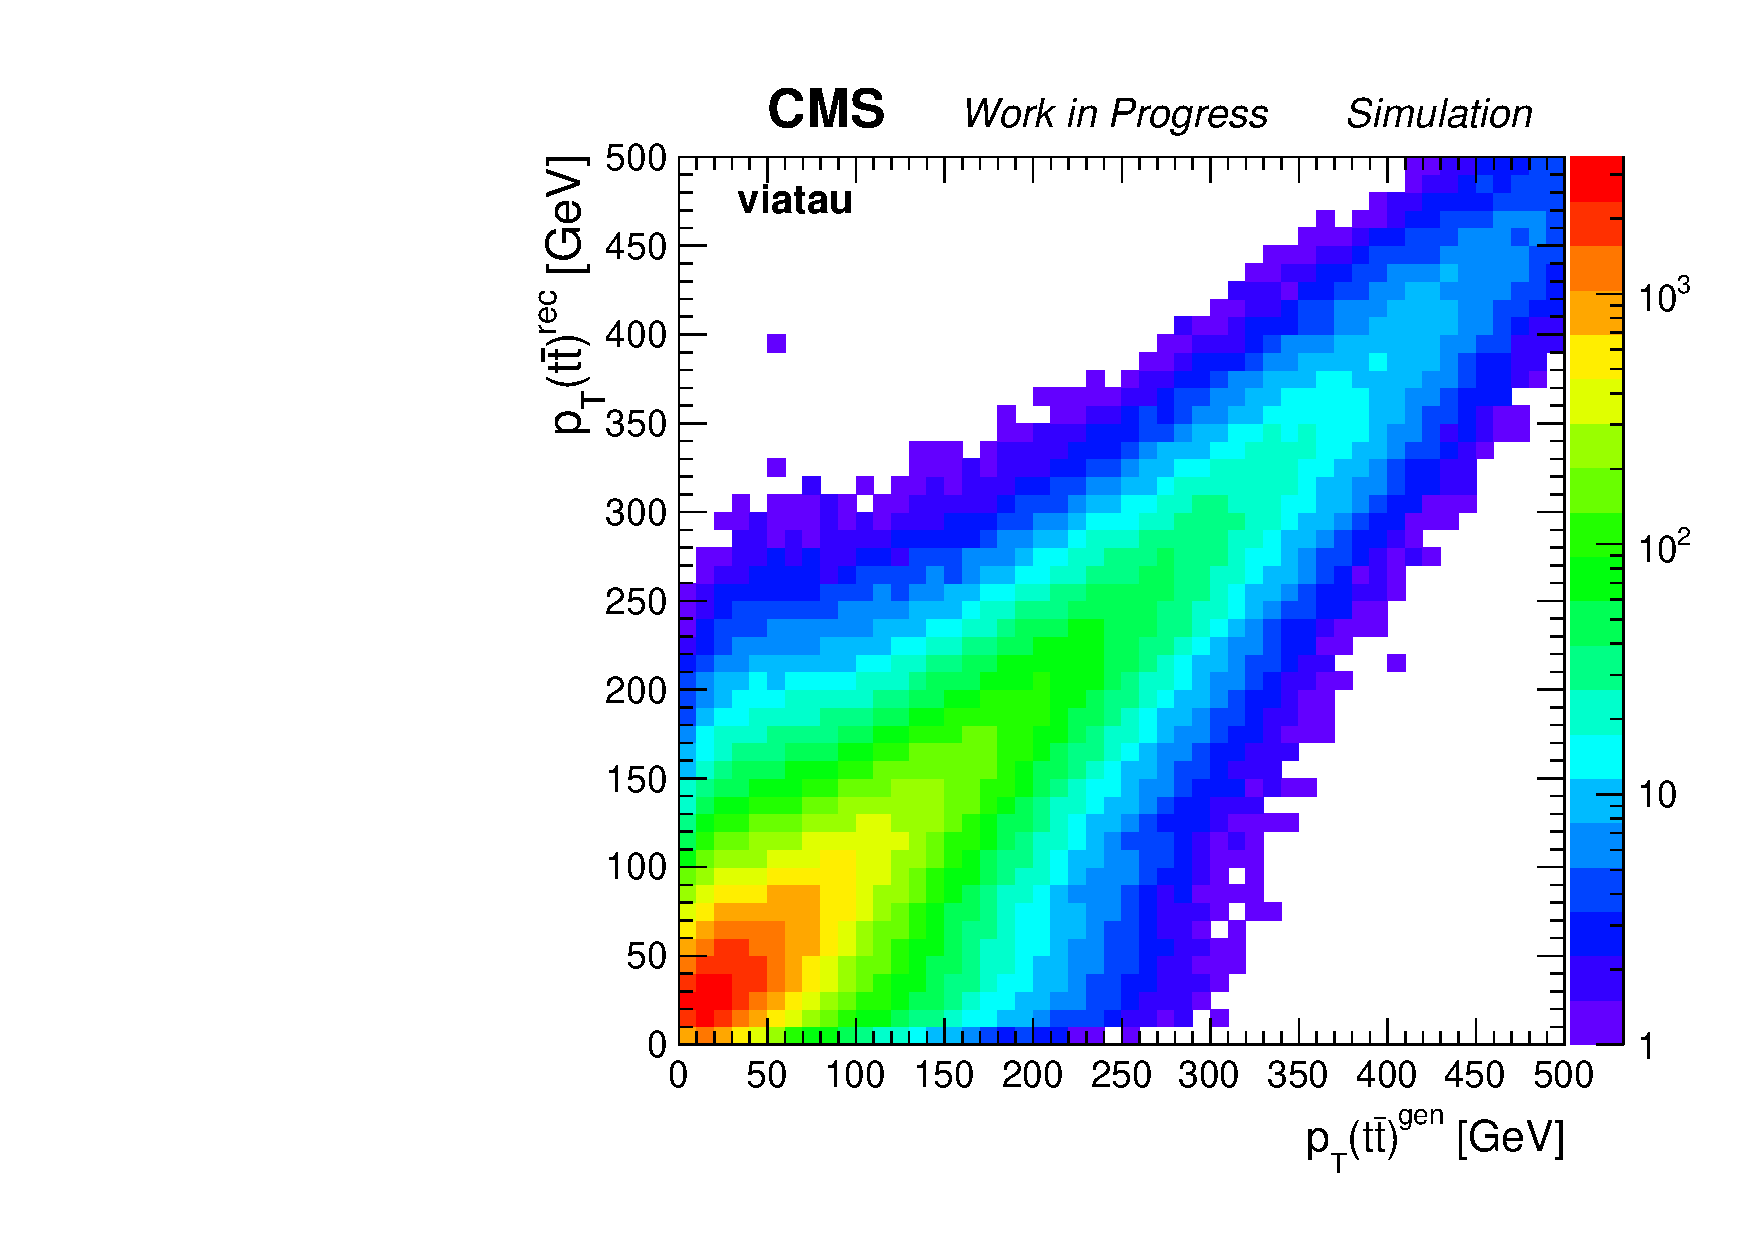
\includegraphics[width=0.30\textwidth]{fig_fullRun2UL/KinRecoResolutions/ttbar_pT_genreco_viatau.pdf}\\
    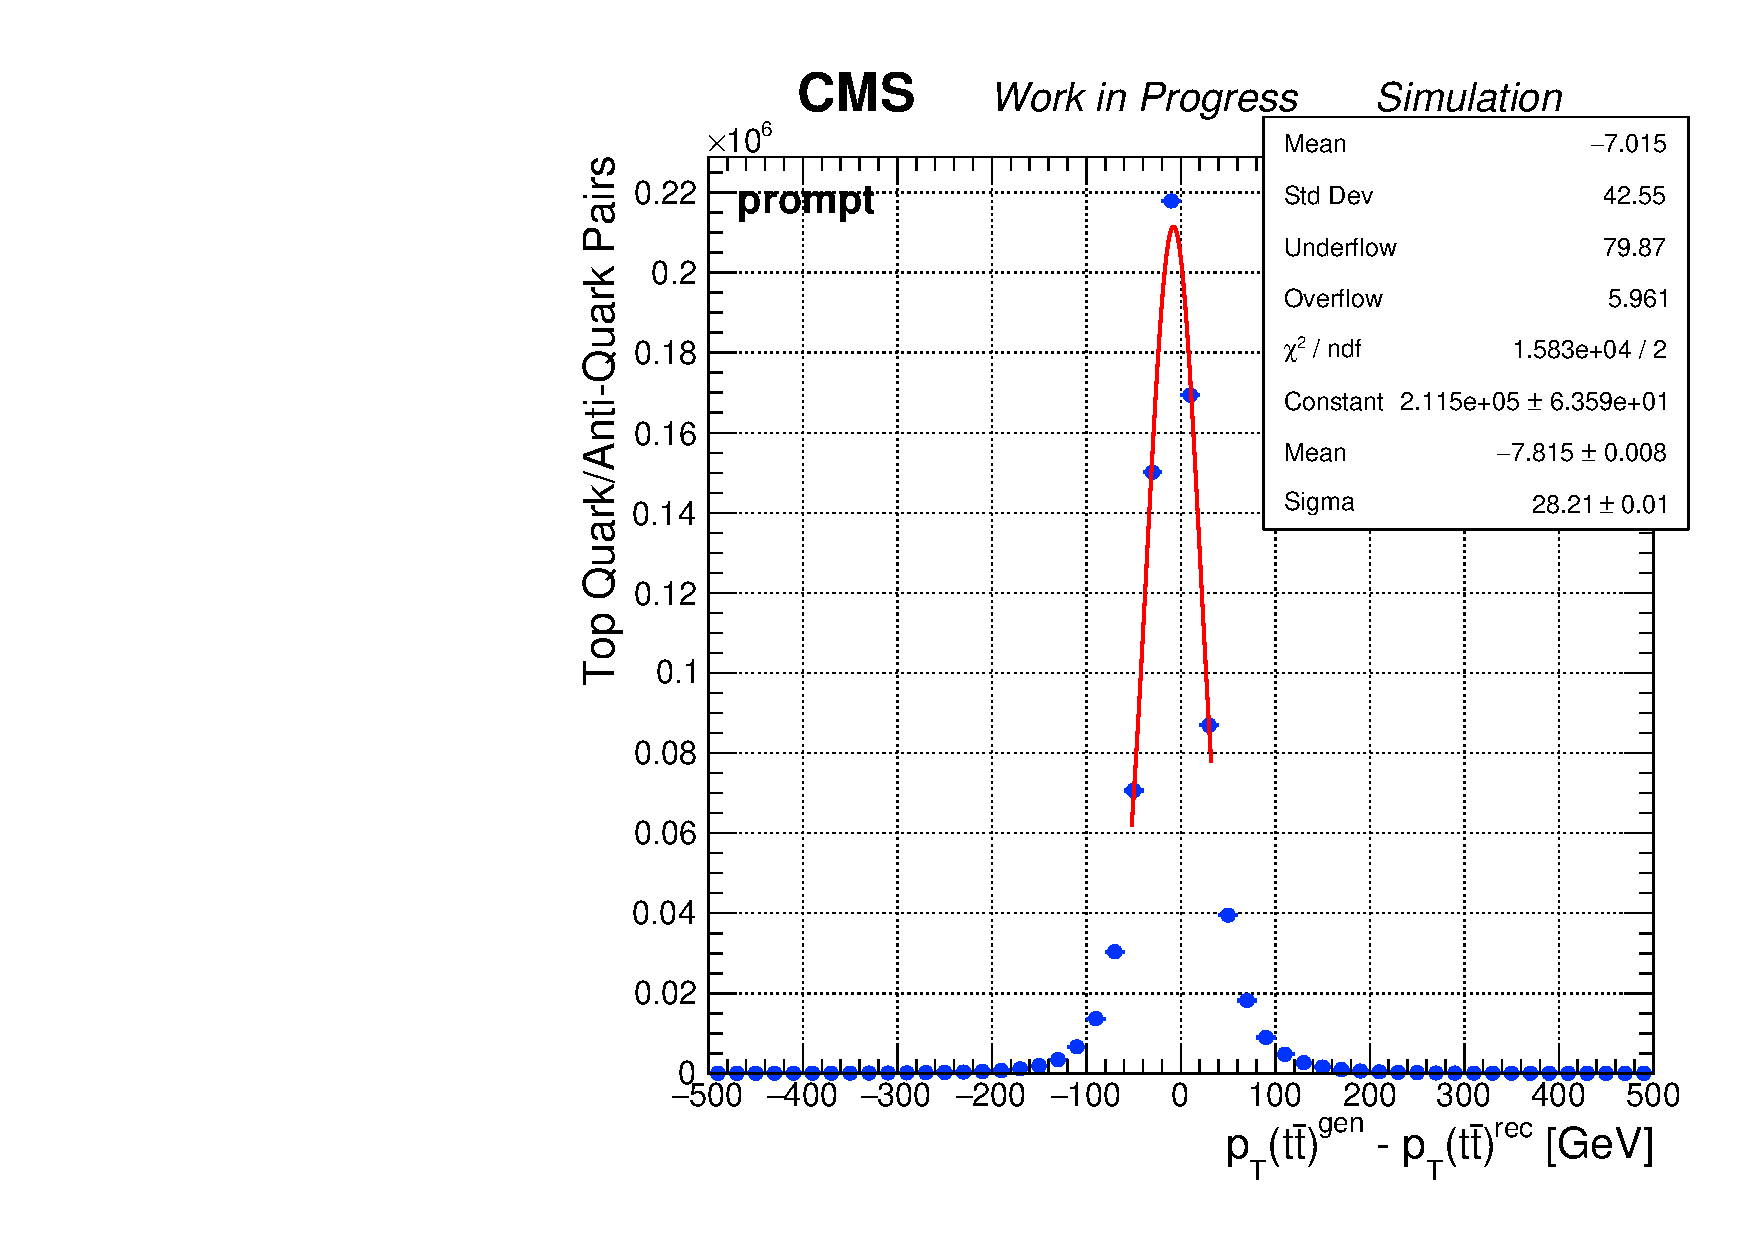
\includegraphics[width=0.30\textwidth]{fig_fullRun2UL/KinRecoResolutions/ttbar_pT_residual_prompt.pdf}
    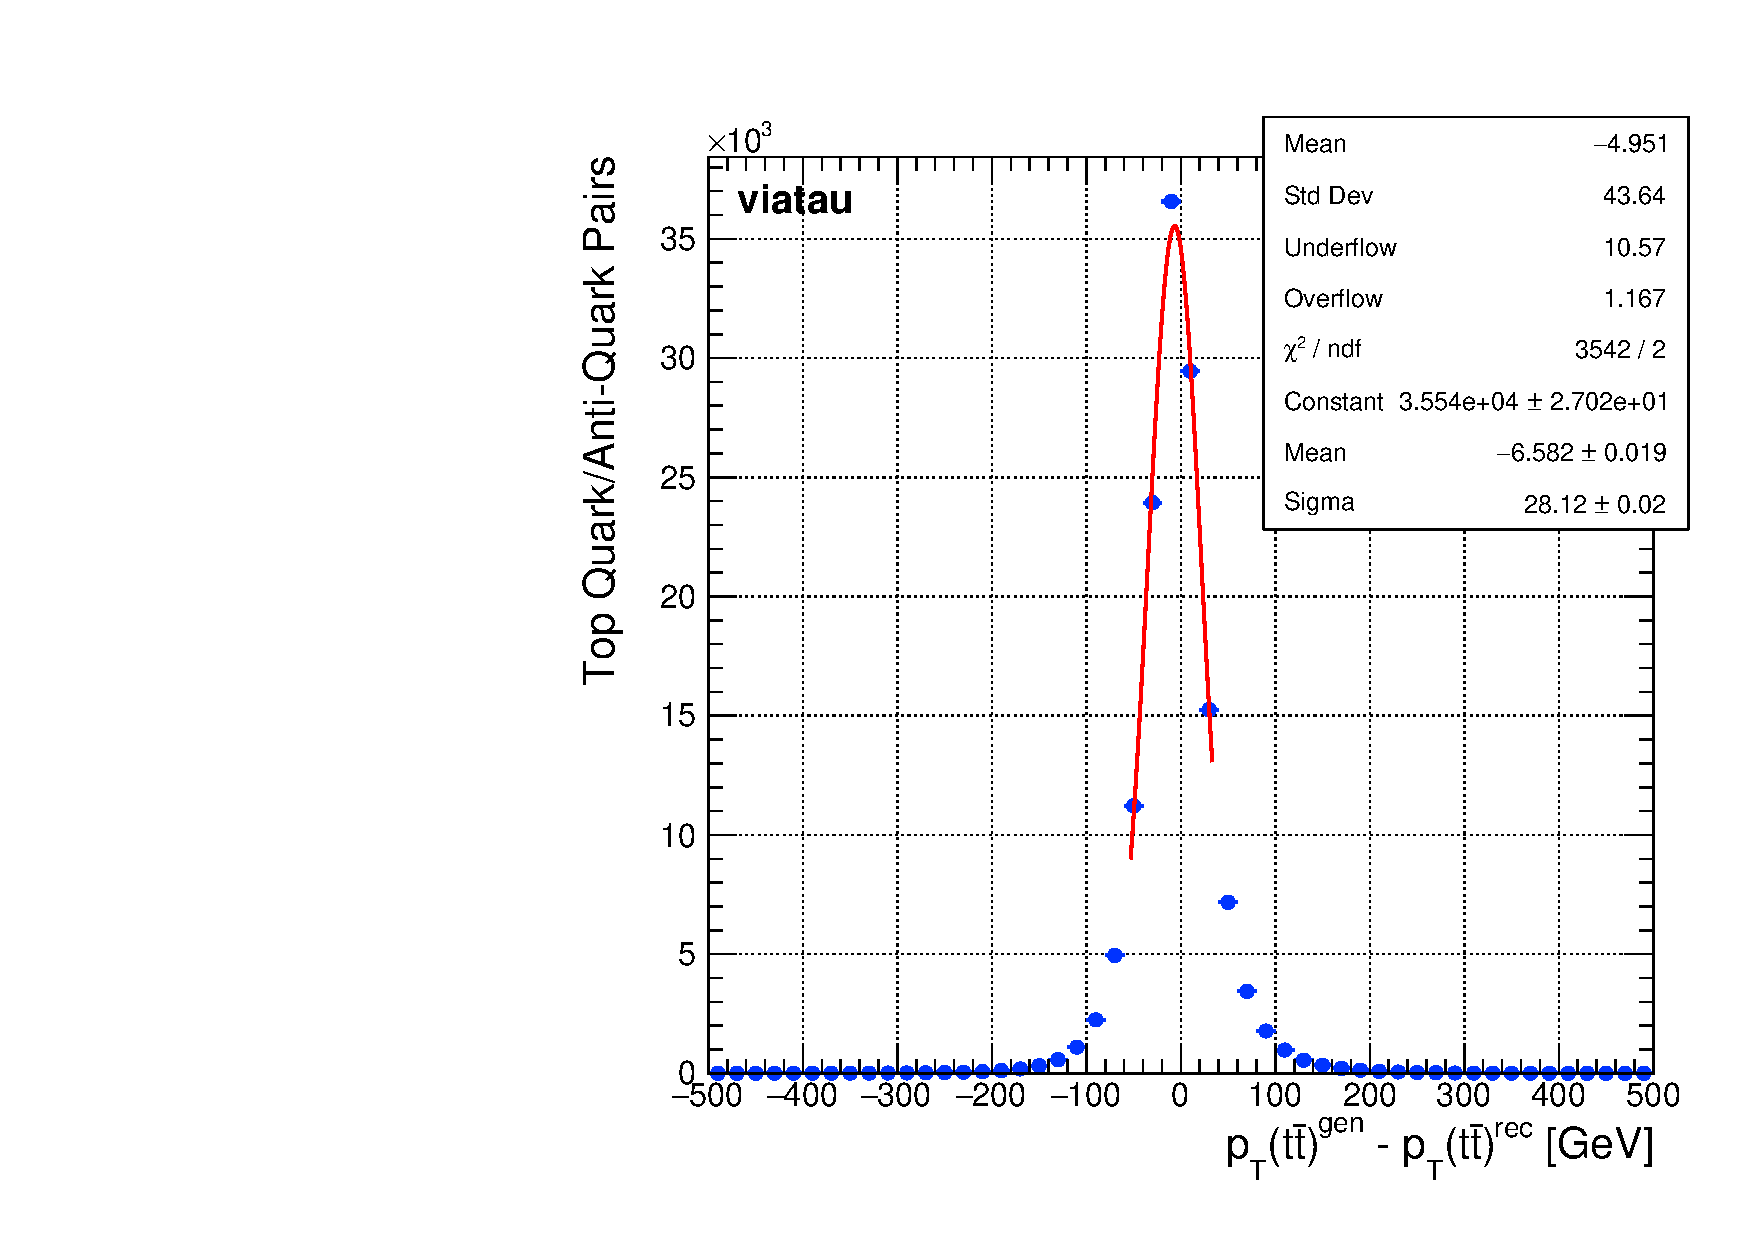
\includegraphics[width=0.30\textwidth]{fig_fullRun2UL/KinRecoResolutions/ttbar_pT_residual_viatau.pdf}\\
    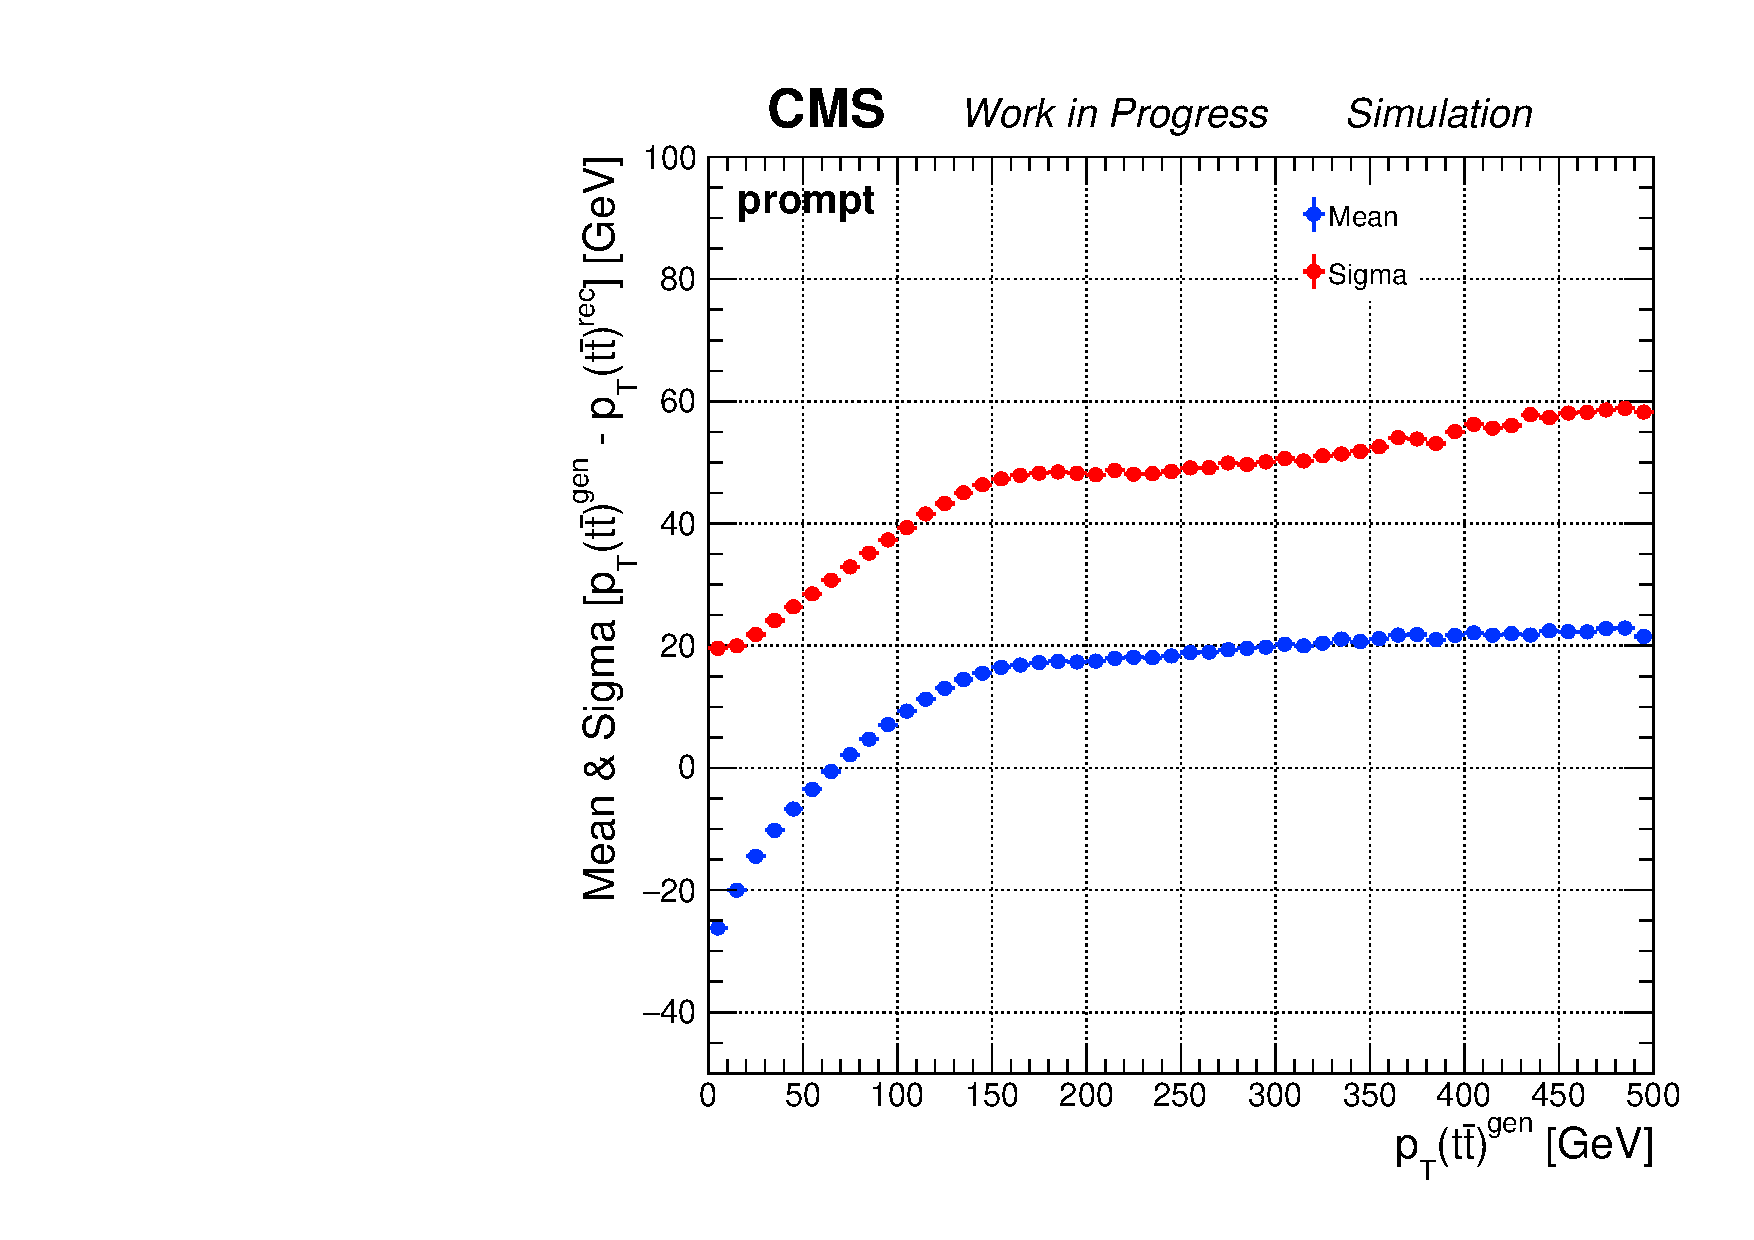
\includegraphics[width=0.30\textwidth]{fig_fullRun2UL/KinRecoResolutions/ttbar_pT_multiresidual_prompt.pdf}
    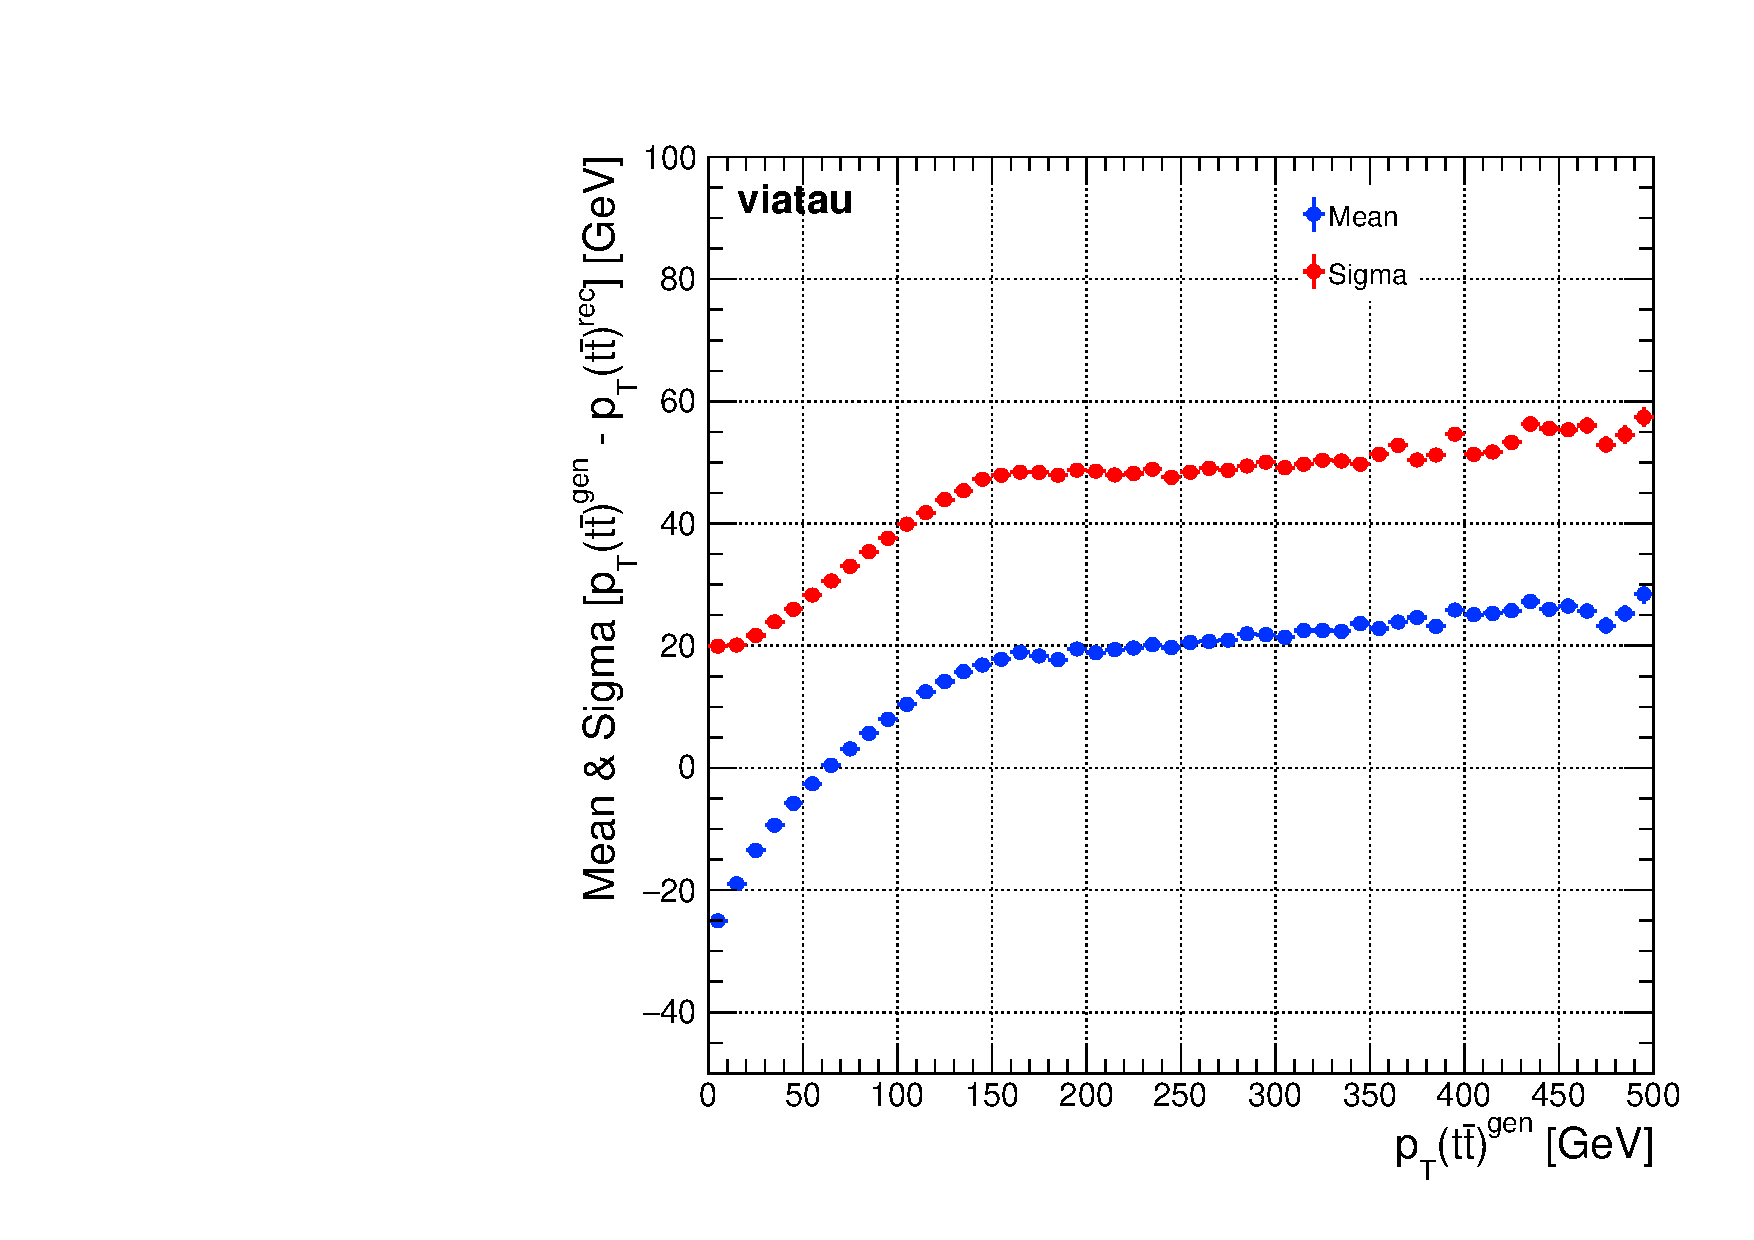
\includegraphics[width=0.30\textwidth]{fig_fullRun2UL/KinRecoResolutions/ttbar_pT_multiresidual_viatau.pdf}\\
    \caption{\small Top: True and reconstructed \pttt\ obtained for prompt (left) and via tau (right) \ttbar dilepton events.
    Middle: The difference between true and reconstructed \pttt\ in bins of true \pttt\ (fitted with a Gaussian function for illustration).
    Bottom: The differential mean and sigma from Gaussian fits, with respect to true \pttt, of the difference between true and reconstructed \pttt\ obtained for prompt and via tau \ttbar dilepton events.
    The simulated samples are normalized to an integrated luminosity of \lumivalueRuniiUL.}
    \label{fig:kinrec:resolution-pttt}
 \end{center}
\end{figure}

\begin{figure}
  \begin{center}
    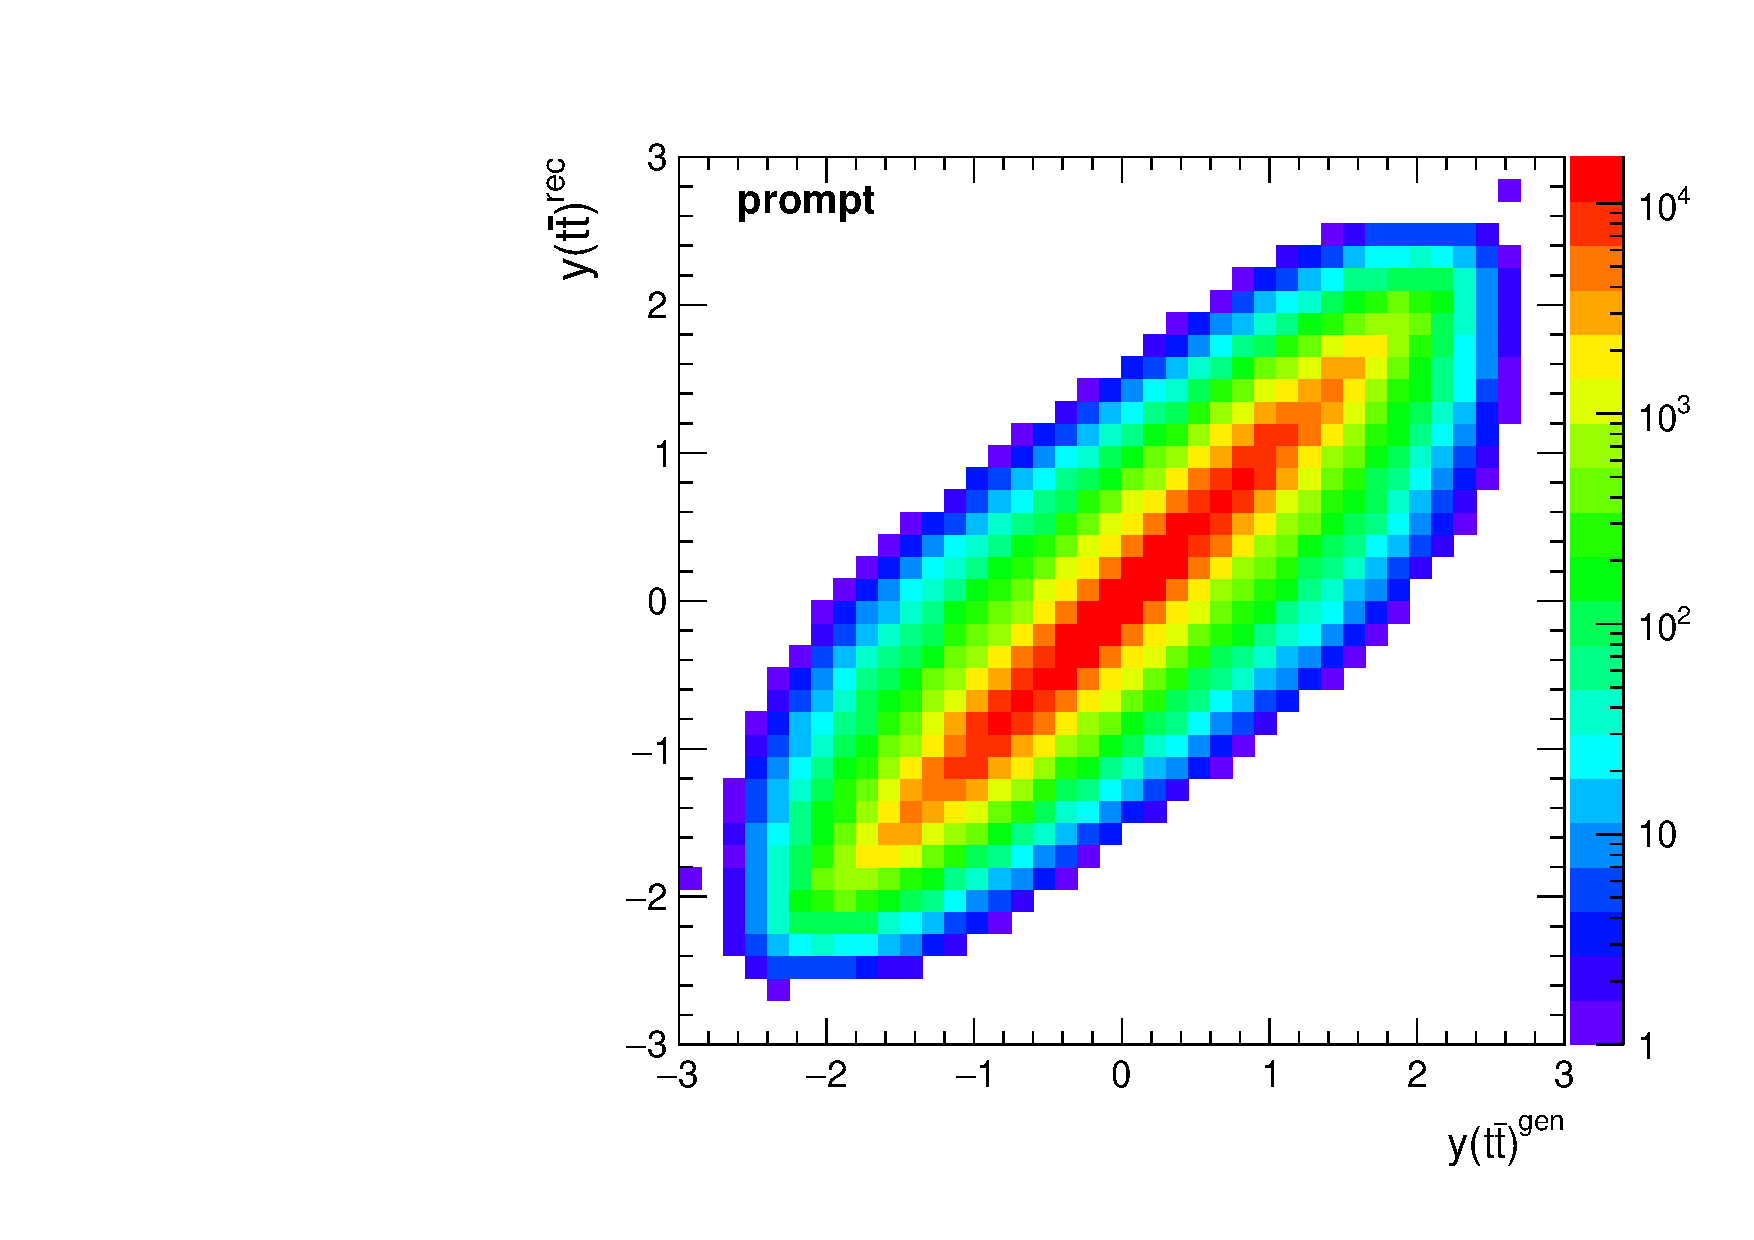
\includegraphics[width=0.30\textwidth]{fig_fullRun2UL/KinRecoResolutions/ttbar_rapidity_genreco_prompt.pdf}
    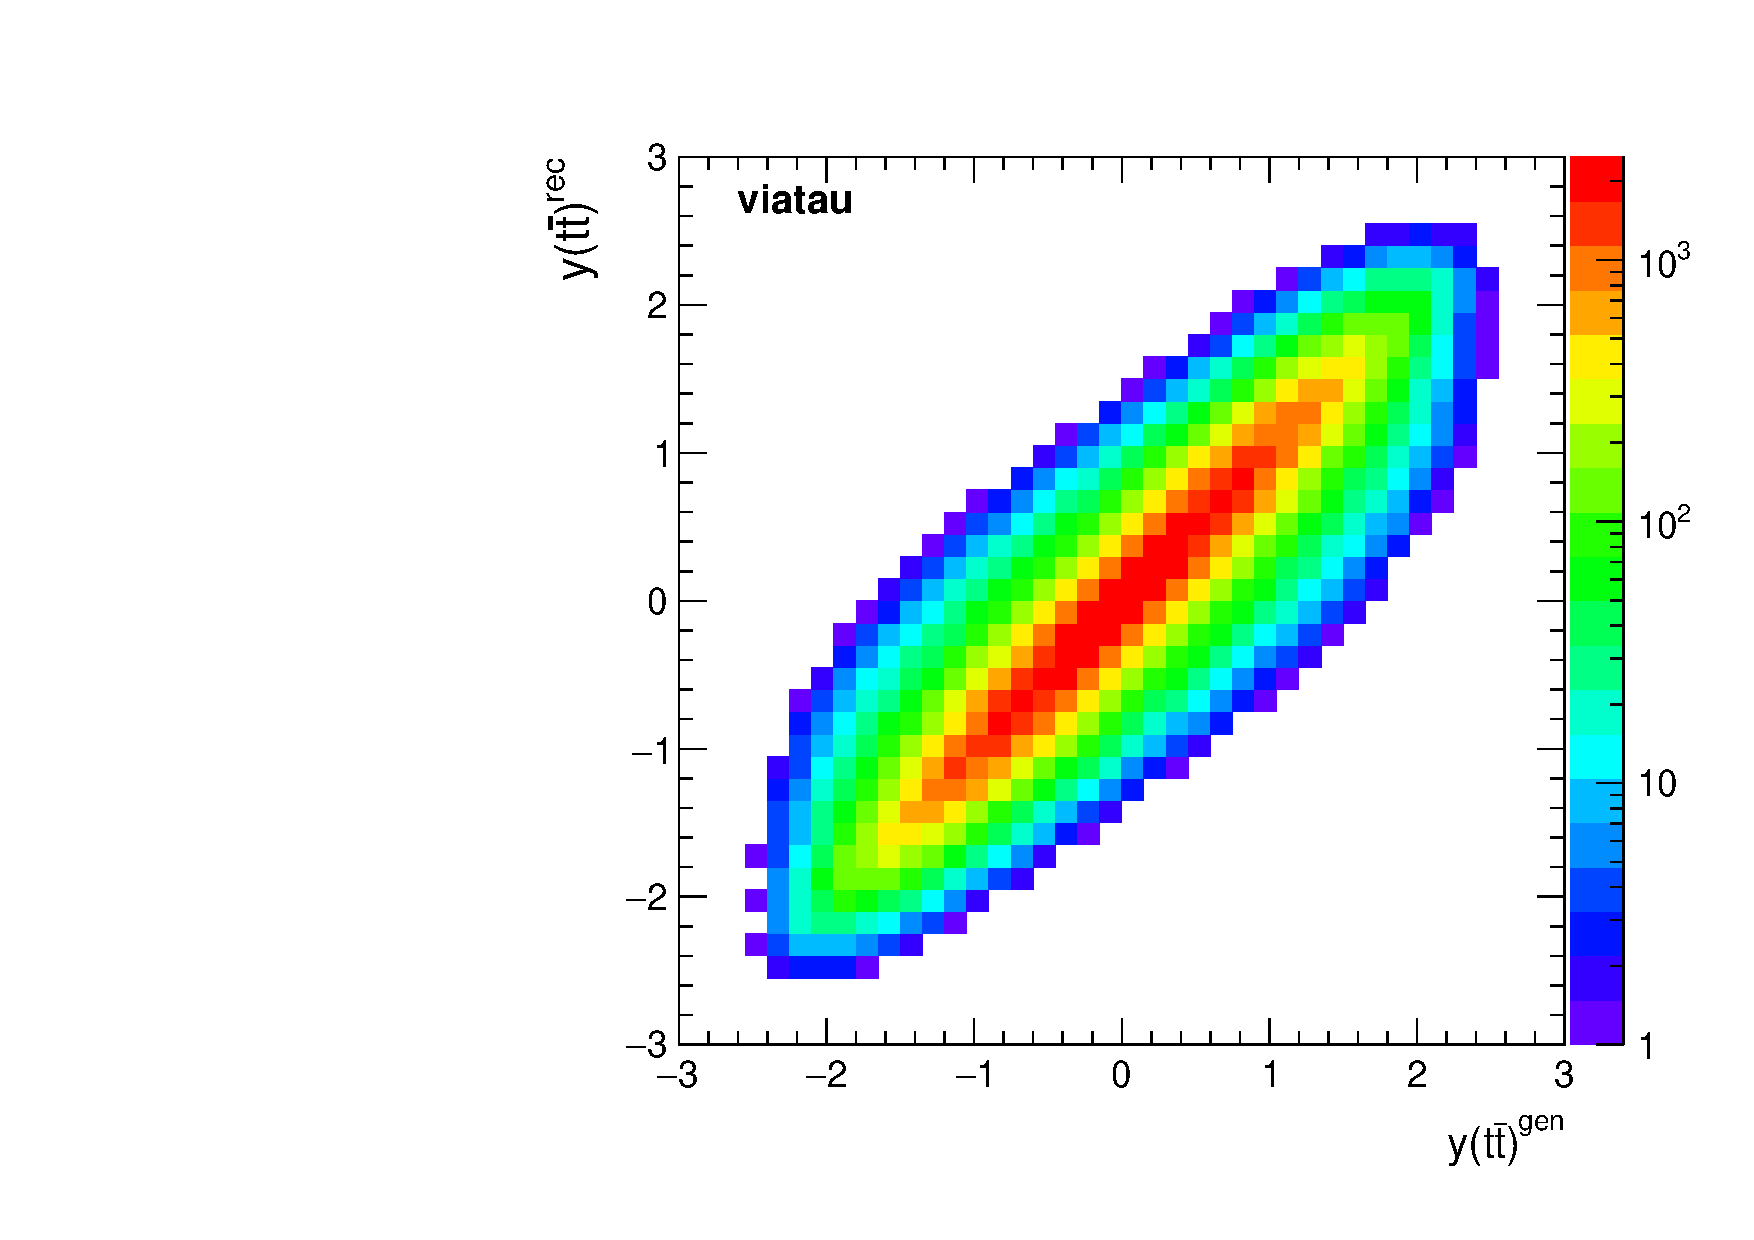
\includegraphics[width=0.30\textwidth]{fig_fullRun2UL/KinRecoResolutions/ttbar_rapidity_genreco_viatau.pdf}\\
    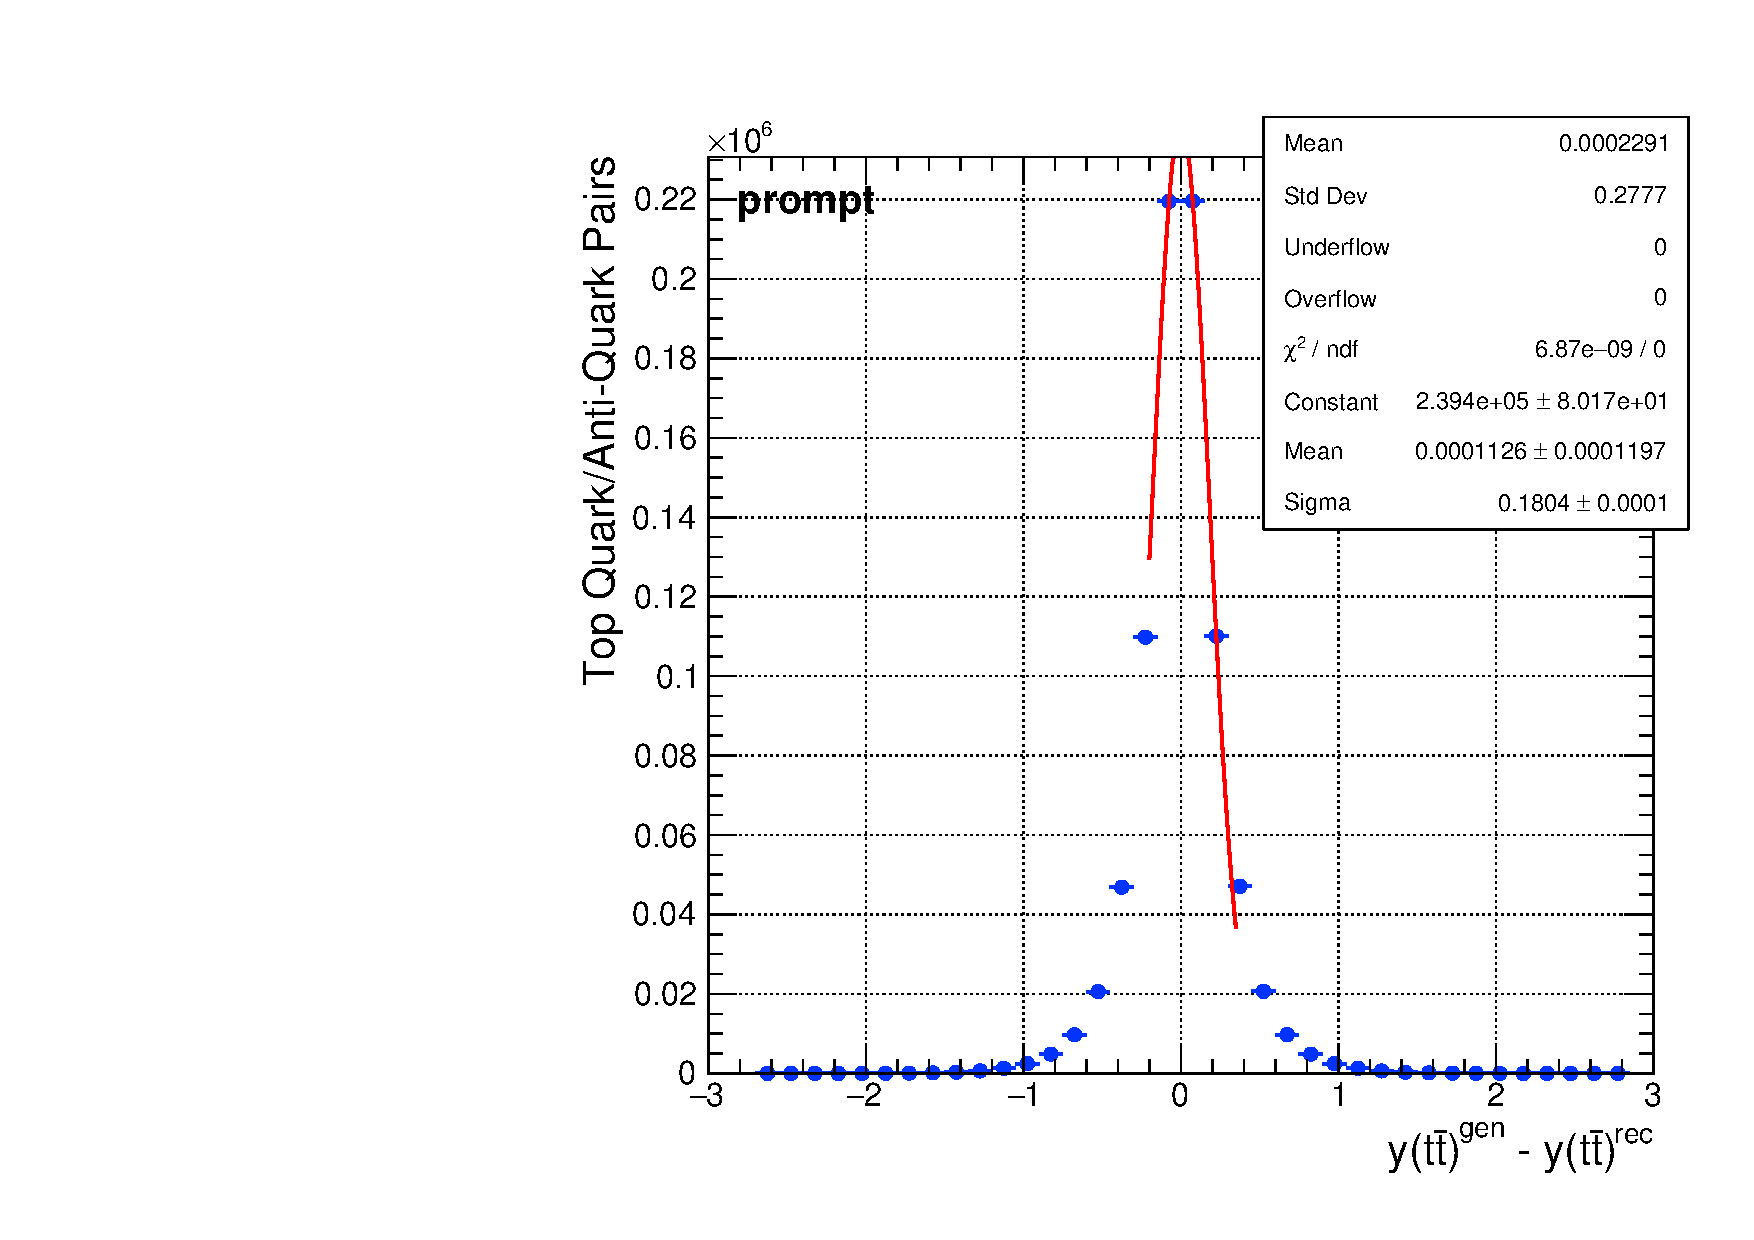
\includegraphics[width=0.30\textwidth]{fig_fullRun2UL/KinRecoResolutions/ttbar_rapidity_residual_prompt.pdf}
    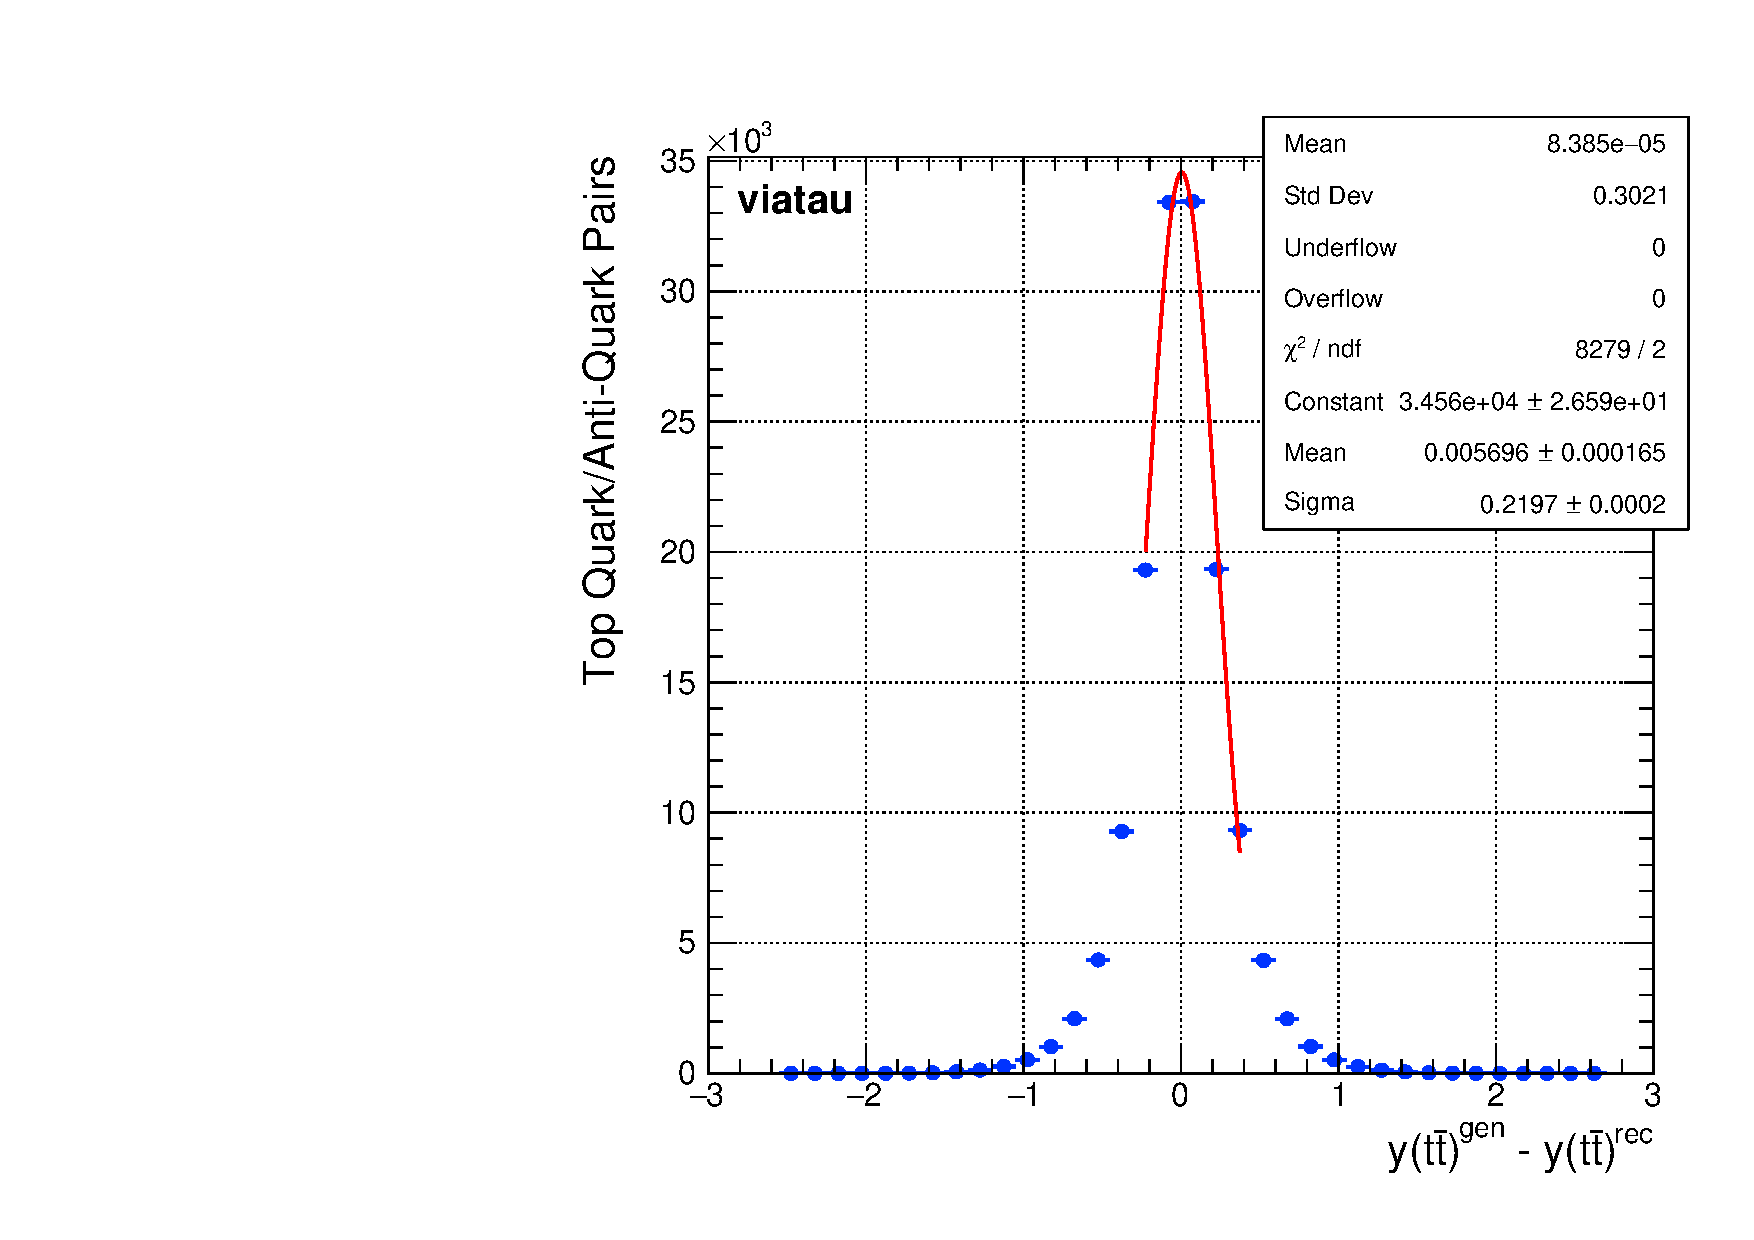
\includegraphics[width=0.30\textwidth]{fig_fullRun2UL/KinRecoResolutions/ttbar_rapidity_residual_viatau.pdf}\\
    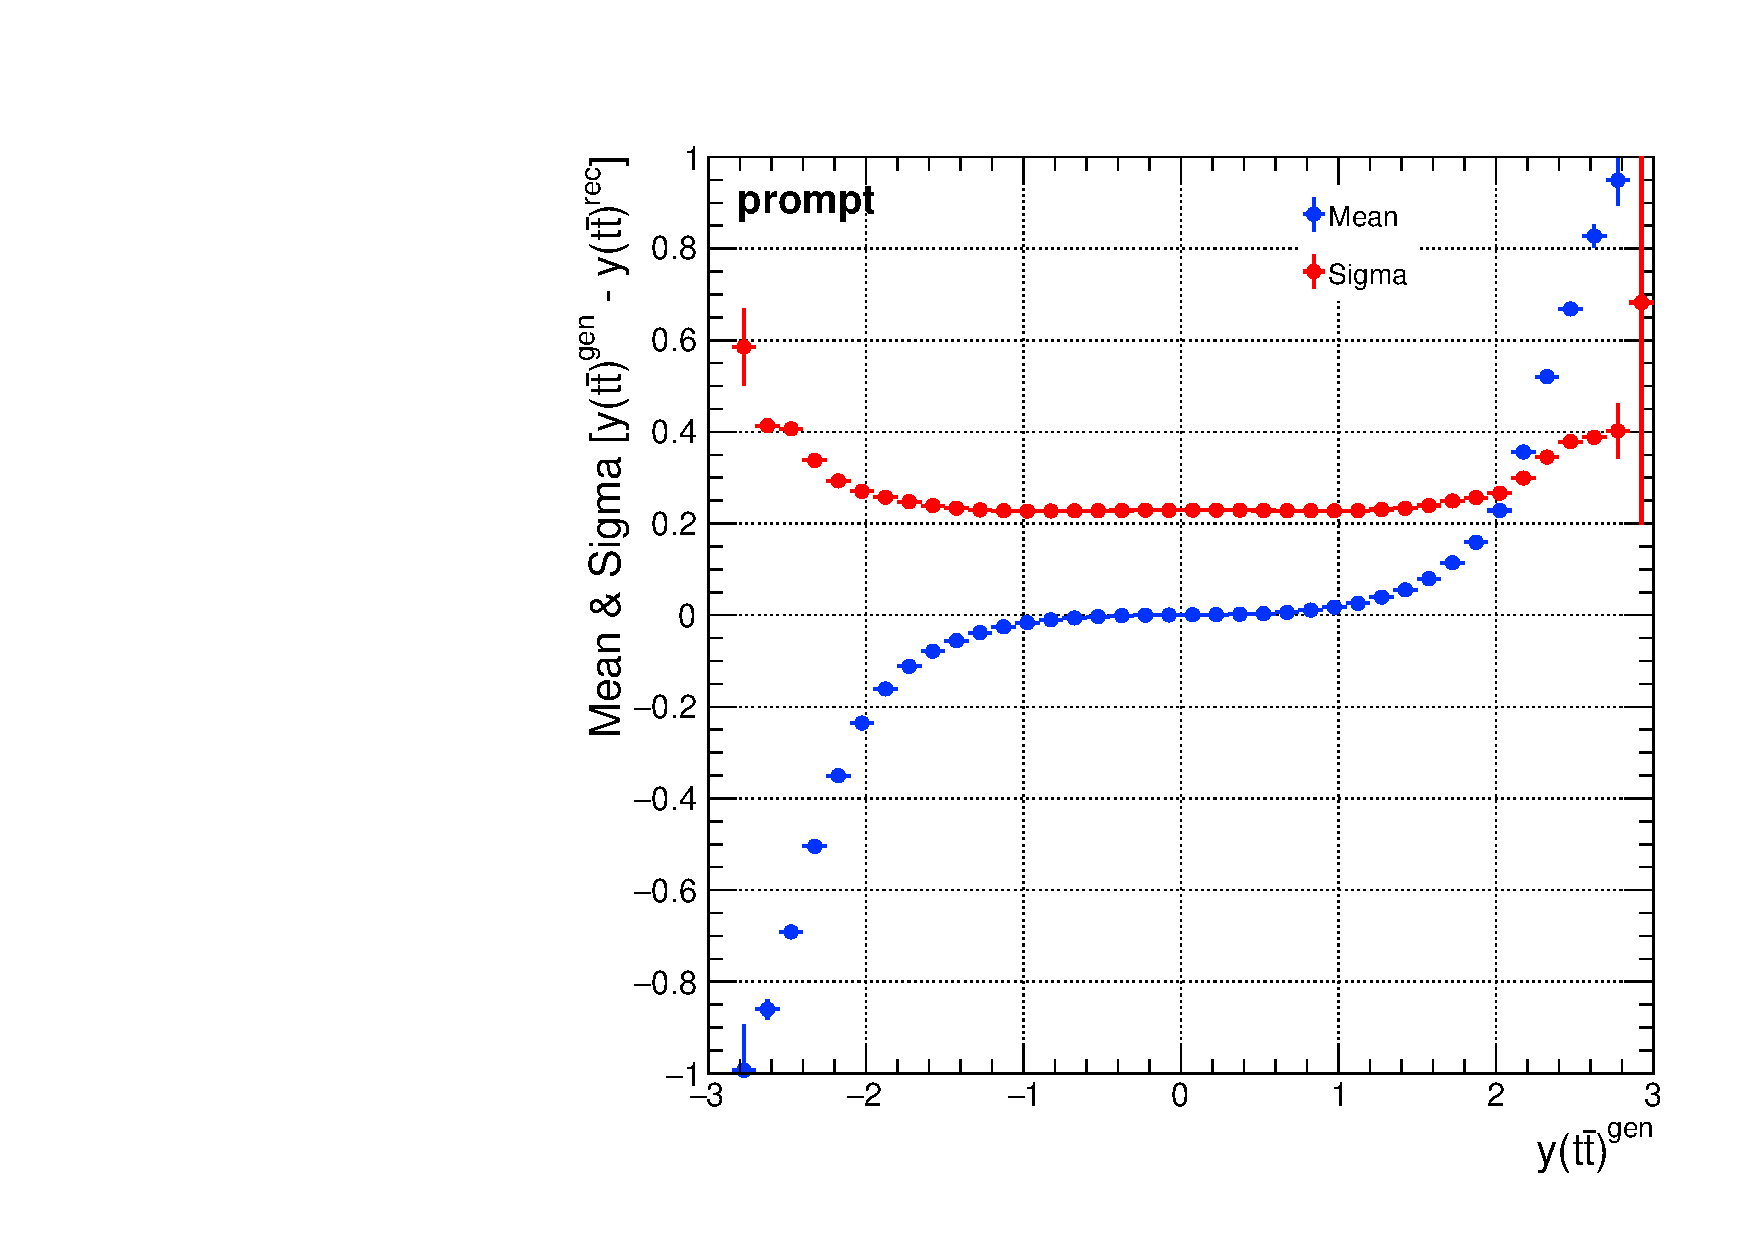
\includegraphics[width=0.30\textwidth]{fig_fullRun2UL/KinRecoResolutions/ttbar_rapidity_multiresidual_prompt.pdf}
    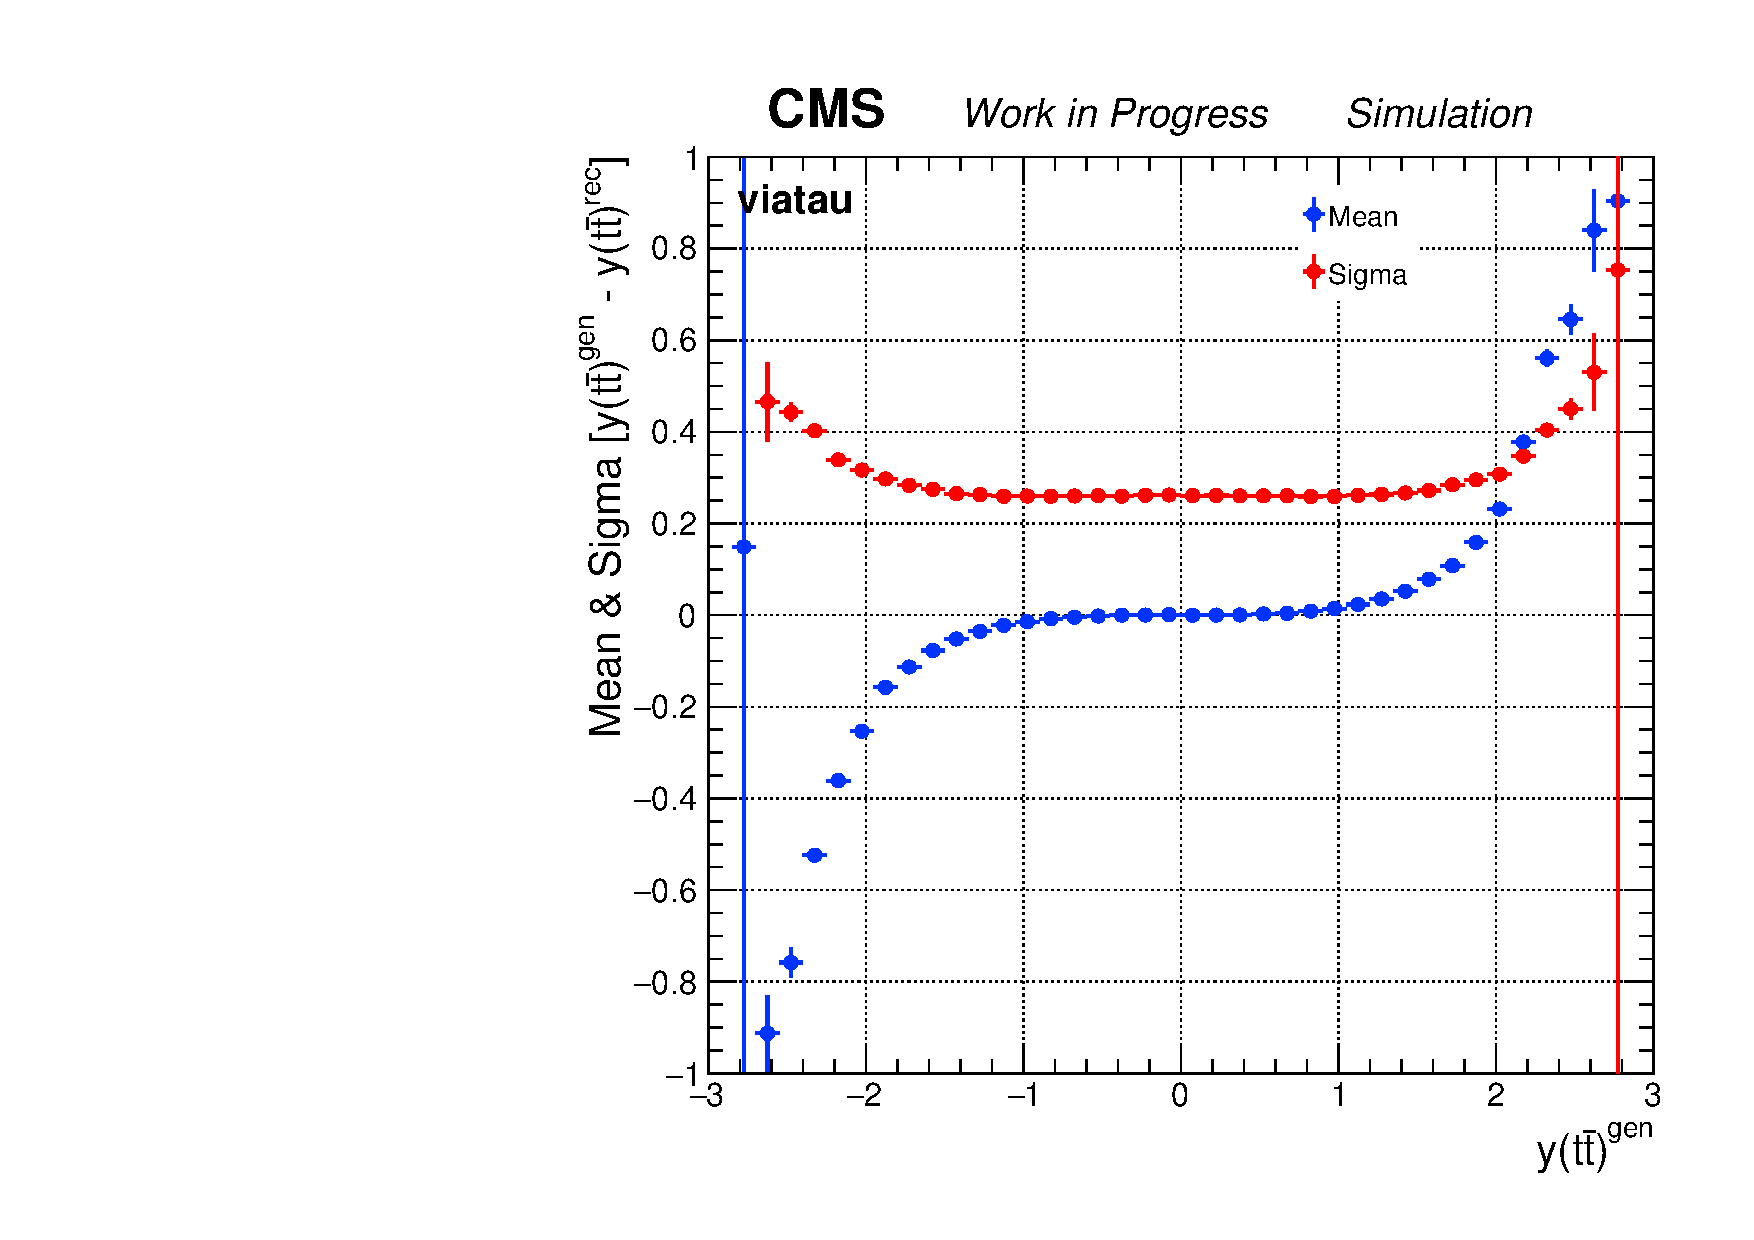
\includegraphics[width=0.30\textwidth]{fig_fullRun2UL/KinRecoResolutions/ttbar_rapidity_multiresidual_viatau.pdf}\\
    \caption{\small Top: True and reconstructed \ytt\ obtained for prompt (left) and via tau (right) \ttbar dilepton events.
    Middle: The difference between true and reconstructed \ytt\ in bins of true \ytt\ (fitted with a Gaussian function for illustration).
    Bottom: The differential mean and sigma from Gaussian fits, with respect to true \ytt, of the difference between true and reconstructed \ytt\ obtained for prompt and via tau \ttbar dilepton events.
    The simulated samples are normalized to an integrated luminosity of \lumivalueRuniiUL.}
    \label{fig:kinrec:resolution-ytt}
 \end{center}
\end{figure}

\begin{figure}
  \begin{center}
    \includegraphics[width=0.30\textwidth]{fig_fullRun2UL/KinRecoResolutions/top_pT_genreco_prompt.pdf}
    \includegraphics[width=0.30\textwidth]{fig_fullRun2UL/KinRecoResolutions/top_pT_genreco_viatau.pdf}\\
    \includegraphics[width=0.30\textwidth]{fig_fullRun2UL/KinRecoResolutions/top_pT_residual_prompt.pdf}
    \includegraphics[width=0.30\textwidth]{fig_fullRun2UL/KinRecoResolutions/top_pT_residual_viatau.pdf}\\
    \includegraphics[width=0.30\textwidth]{fig_fullRun2UL/KinRecoResolutions/top_pT_multiresidual_prompt.pdf}
    \includegraphics[width=0.30\textwidth]{fig_fullRun2UL/KinRecoResolutions/top_pT_multiresidual_viatau.pdf}\\
    \caption{\small Top: True and reconstructed \ptt\ obtained for prompt (left) and via tau (right) \ttbar dilepton events.
    Middle: The difference between true and reconstructed \ptt\ in bins of true \ptt\ (fitted with a Gaussian function for illustration).
    Bottom: The differential mean and sigma from Gaussian fits, with respect to true \ptt, of the difference between true and reconstructed \ptt\ obtained for prompt and via tau \ttbar dilepton events.
    The simulated samples are normalized to an integrated luminosity of \lumivalueRuniiUL.}
    \label{fig:kinrec:resolution-ptt}
 \end{center}
\end{figure}

\begin{figure}
  \begin{center}
    \includegraphics[width=0.30\textwidth]{fig_fullRun2UL/KinRecoResolutions/top_rapidity_genreco_prompt.pdf}
    \includegraphics[width=0.30\textwidth]{fig_fullRun2UL/KinRecoResolutions/top_rapidity_genreco_viatau.pdf}\\
    \includegraphics[width=0.30\textwidth]{fig_fullRun2UL/KinRecoResolutions/top_rapidity_residual_prompt.pdf}
    \includegraphics[width=0.30\textwidth]{fig_fullRun2UL/KinRecoResolutions/top_rapidity_residual_viatau.pdf}\\
    \includegraphics[width=0.30\textwidth]{fig_fullRun2UL/KinRecoResolutions/top_rapidity_multiresidual_prompt.pdf}
    \includegraphics[width=0.30\textwidth]{fig_fullRun2UL/KinRecoResolutions/top_rapidity_multiresidual_viatau.pdf}\\
    \caption{\small Top: True and reconstructed \yt\ obtained for prompt (left) and via tau (right) \ttbar dilepton events.
    Middle: The difference between true and reconstructed \yt\ in bins of true \yt\ (fitted with a Gaussian function for illustration).
    Bottom: The differential mean and sigma from Gaussian fits, with respect to true \yt, of the difference between true and reconstructed \yt\ obtained for prompt and via tau \ttbar dilepton events.
    The simulated samples are normalized to an integrated luminosity of \lumivalueRuniiUL.}
    \label{fig:kinrec:resolution-yt}
 \end{center}
\end{figure}


\section{\ensuremath{\mathrm{Z+Jets}} Background Determination}
The expected background contributions from \ttbar, $tW$, \wjets, and diboson processes are directly taken from the MC simulations.
The \zjets\ background contribution in the selected phase space is not modeled accurately in MC simulations, and the normalization of the \zjets\ background contribution corrected using global normalization scale factors, which are determined from a binned template fit to the data using TFractionFitter as described in~\cite{CMS-PAS-TOP-20-006}\cite{BARLOW1993219}.
TFractionFitter is a class in the ROOT~\cite{Antcheva:2011zz} data analysis framework that performs a simultaneous binned Poisson maximum likelihood fit of multiple MC templates in order to determine the linear combination of templates and fractions that best describe the recorded data. 
Within the vetoed $Z$ boson mass peak control region $\SI{76}{\GeV} < \mll < \SI{106}{\GeV}$, MC templates obtained from the MC simulated samples for \zjets\ processes $\text{T}_{\zjets}$ and the sum of all other MC contributions $\text{T}_\text{Other}$ are fitted to the \mll distributions in the data template $\text{T}_\text{Data}$ as:
\begin{linenomath*}
\begin{align}
\text{T}_\text{Data} = f_{\zjets} \cdot \text{T}_{\zjets} + f_{\text{Other}} \cdot \text{T}_\text{Other}
\end{align}
\end{linenomath*}
where $f_{\zjets}$ and $f_{\text{Other}}$ are the fractions obtained from the fit.
Separate global normalization scale factors ($\mathcal{SF}$) are fitted in the \ee and \mumu channels:
\begin{linenomath*}
\begin{align}
\mathcal{SF}_{ee} &= \frac{f_{\zjets}^{\ee} \cdot N_\text{Data}^{\ee}}{N_{\zjets}^{\ee}} \\
\mathcal{SF}_{\mu\mu} &= \frac{f_{\zjets}^{\mumu} \cdot N_\text{Data}^{\mumu}}{N_{\zjets}^{\mumu}}
\end{align}
\end{linenomath*}
where $N_{\zjets}$ and $N_\text{Data}$ are the number of events in the \zjets\ template and data distribution.
The \emu and combined channel scale factors are calculated as:
\begin{linenomath*}
\begin{gather}
\mathcal{SF}_{\emu} = \sqrt{\mathcal{SF}_{\ee} \times \mathcal{SF}_{\mumu}} \\
\mathcal{SF}_{\ell \bar{\ell}} = \frac{\mathcal{SF}_{\ee} \cdot N_\text{Data}^{\ee} + \mathcal{SF}_{\mumu} \cdot N_\text{Data}^{\mumu} + \mathcal{SF}_{\emu} \cdot N_\text{Data}^{\emu}}{N_\text{Data}^{\ee} + N_\text{Data}^{\mumu} + N_\text{Data}^{\emu}}.
\end{gather}
\end{linenomath*}
To enhance \zjets\ statistics in the orthogonal phase space of the $Z$ boson mass peak control region, \MET and b-tagging event selection requirements are omitted, as is the requirement of a kinematic reconstruction solution.
The fits performed by TFractionFitter of the two MC templates to the data template within the $Z$ boson mass peak control region are shown for Full Run II in figure~\ref{fig:fitstatusfullRun2UL}
The resulting \zjets\ global normalization scale factors are shown in table~\ref{tab:dysffullRun2UL}.

\begin{figure}[!htb]
  \begin{center}
        \includegraphics[width=0.30\textwidth]{fig_fullRun2UL/fit_status_ee.pdf}
        \includegraphics[width=0.30\textwidth]{fig_fullRun2UL/fit_status_mumu.pdf}
        \caption{
            \small Dilepton mass distributions in the $Z$ boson mass peak control between $\SI{76}{\GeV} < \mll < \SI{106}{\GeV}$ are shown for the \ee (left) and \mumu (right) channels for Full Run II. 
            The data template $\text{T}_\text{Data}$ is illustrated by black dots, the \zjets\ template $\text{T}_{\zjets}$ is shown in blue, and the sum of all other MC contributions template $\text{T}_\text{Other}$ is green. 
            The red histogram shows the result of the fit performed by TFractionFitter.
            \label{fig:fitstatusfullRun2UL}
    }
  \end{center}
\end{figure}

\begin{table}[!htb]
 \begin{center}
    \begin{tabular}{|c|cccc|}
      \hline 
      \multicolumn{5}{|c|}{\zjets\ Global Normalization Scale Factors} \\
      \hline 
                 & $\mathcal{SF}_{\ee}$ & $\mathcal{SF}_{\mumu}$ & $\mathcal{SF}_{\emu}$ & $\mathcal{SF}_{\ell \bar{\ell}}$ \\
      \hline
      2016preVFP & $1.081 \pm 0.005$ & $1.071 \pm 0.004$ & $1.076 \pm 0.013$ & $1.074 \pm 0.019$ \\
      2016postVFP & $1.112 \pm 0.006$ & $1.144 \pm 0.004$ & $1.128 \pm 0.015$ & $1.133 \pm 0.021$ \\
      2017 & $1.078 \pm 0.004$ & $1.103 \pm 0.002$ & $1.091 \pm 0.009$ & $1.095 \pm 0.012$ \\
      2018 & $1.042 \pm 0.003$ & $1.047 \pm 0.002$ & $1.044 \pm 0.007$ & $1.045 \pm 0.01$ \\
      Full Run II  & $1.067 \pm 0.002$ & $1.079 \pm 0.001$ & $1.073 \pm 0.005$ & $1.075 \pm 0.007$ \\
      \hline
    \end{tabular}
  \caption{Data-driven \zjets\ global normalization scale factors $\pm$ the statistical uncertainty from the fit, determined within the vetoed $Z$ boson mass peak control region $\SI{76}{\GeV} < \mll < \SI{106}{\GeV}$ using TFractionFitter.}
  \label{tab:dysffullRun2UL}     
 \end{center}
\end{table}


\section{Event Yields}
The eight consecutive event selection steps are summarized as:
\begin{itemize}
    \item {\bf MET Filters:} Events that are not excluded due to MET filters ({\bf 1a}),
    \item {\bf Triggers:} Events that pass trigger requirements ({\bf 1b}),
    \item {\bf Primary Vertex:} Events with primary vertex passing selection requirements ({\bf 1}),
    \item {\bf Leptons:} Events with exactly two oppositely-charged isolated leptons ({\bf 2}) and $m_{\ell\ell} > \SI{20}{\GeV}$ ({\bf 3}).  
            In the \mumu and \ee channels, the \zjets\ background is removed by rejecting events in the Z boson mass region $\SI{76}{\GeV} < m^{\ell\bar{\ell}} < \SI{106}{\GeV}$ ({\bf 4}),
    \item {\bf Jets:} Events with at least two jets fulfilling the jet \pT and $\eta$ requirements ({\bf 5}),
    \item {\bf Missing Transverse Energy:} Events in the \mumu and \ee channels with $\ETmiss > \SI{40}{\GeV}$ ({\bf 6}),
    \item {\bf b-Tagging:} Events include at least one b-tagged jet ({\bf 7}),
    \item {\bf Top Pair Reconstruction:} Events with at least one physically meaningful solution for the full kinematic reconstruction of a \ttbar\ system ({\bf 8}).
\end{itemize}
The numbers of observed events in the data compared to the expected events from MC simulation for Full Run II are given in Table~\ref{t-cutflowfullRun2UL} after each of the consecutive selection steps.

\begin{table}[!htb]
 \begin{center}
    \caption{\small Full Run II (\lumivalueRuniiUL) expected event yields for signal and background processes, compared to the event yields in recorded data, after each step of event selection.} 
    \label{t-cutflowfullRun2UL}
      \begin{adjustbox}{scale=0.70,center}
       {\footnotesize
        \begin{tabular}{lrrrrrrr}
\hline $\boldsymbol{\mu^+\mu^-}$ & Leptons & Jets & \ETmiss & b-Tag & Kin. Reco. \\
\hline
\ttbar\ Signal &                486260.0&               342459.0&               272219.0&               241382.0&               220154.0                \\
\ttbar\ Other &         10796.4&                8293.4&         6237.5&         4266.4&         3544.3          \\
$\ttbar+Z/W$&           1326.0&         1201.9&         988.9&          850.3&          664.0           \\
Single &                49638.5&                19065.8&                15251.4&                12362.2&                8413.4          \\
Diboson &               71079.5&                6822.1&         3549.0&         475.0&          275.8           \\
W+jets &                5268.4&         589.4&          252.8&          78.9&           78.3            \\
Z+jets &                7489000.0&              404230.0&               91862.9&                14070.5&                9951.6          \\
\hline
\textbf{MC Total} &                8113370.0&              782661.0&               390362.0&               273486.0&               \textbf{243081.0}                \\
\textbf{Data} &          8060660.0&              797354.0&               405879.0&               278054.0&               \textbf{247150.0}                \\
\hline
\hline $\boldsymbol{\mu^{\pm}}\mathbf{e^{\mp}}$ & Leptons & Jets & \ETmiss & b-Tag & Kin. Reco. \\
\hline
\ttbar\ Signal &                896402.0&               633218.0&               633218.0&               562837.0&               520593.0                \\
\ttbar\ Other &         15438.4&                11944.2&                11944.2&                8448.5&         7157.5          \\
$\ttbar+Z/W$&           2174.8&         1954.3&         1954.3&         1676.3&         1382.2          \\
Single &                90803.8&                34783.6&                34783.6&                28290.6&                20105.7         \\
Diboson &               111527.0&               6568.6&         6568.6&         773.8&          475.7           \\
W+jets &                17722.3&                1904.9&         1904.9&         354.6&          248.2           \\
Z+jets &                269816.0&               17614.8&                17614.8&                2297.5&         1803.2          \\
\hline
\textbf{MC Total} &                1403880.0&              707988.0&               707988.0&               604679.0&               \textbf{551765.0}                \\
\textbf{Data} &          1441170.0&              710103.0&               710103.0&               598682.0&               \textbf{546299.0}                \\
\hline
\hline $\mathbf{e^{+}e^{-}}$ & Leptons & Jets & \ETmiss & b-Tag & Kin. Reco. \\
\hline
\ttbar\ Signal &                257108.0&               181548.0&               144446.0&               127904.0&               115659.0                \\
\ttbar\ Other &         2370.2&         1855.0&         1405.8&         1083.1&         943.4           \\
$\ttbar+Z/W$&           742.8&          675.2&          551.2&          469.2&          356.6           \\
Single &                26190.4&                10211.3&                8179.1&         6673.7&         4369.0          \\
Diboson &               35619.4&                3645.2&         1920.4&         264.2&          150.9           \\
W+jets &                5859.0&         454.1&          321.0&          13.3&           0.0             \\
Z+jets &                3282680.0&              191128.0&               42368.6&                6563.1&         4360.6          \\
\hline
\textbf{MC Total} &                3610570.0&              389517.0&               199192.0&               142971.0&               \textbf{125840.0}                \\
\textbf{Data} &          3535030.0&              388972.0&               201114.0&               140293.0&               \textbf{123471.0}              \\
\hline
\hline $\boldsymbol{\ell \bar{\ell}}$ & Leptons & Jets & \ETmiss & b-Tag & Kin. Reco. \\
\hline
\ttbar\ Signal &                1639770.0&              1157230.0&              1049880.0&              932124.0&               856406.0                \\
\ttbar\ Other &         28605.1&                22092.6&                19587.5&                13797.9&                11645.2         \\
$\ttbar+Z/W$&           4243.7&         3831.4&         3494.4&         2995.8&         2402.8          \\
Single &                166633.0&               64060.7&                58214.0&                47326.4&                32888.1         \\
Diboson &               218226.0&               17035.9&                12038.0&                1513.0&         902.4           \\
W+jets &                28849.8&                2948.4&         2478.7&         446.8&          326.5           \\
Z+jets &                11041500.0&             612934.0&               151855.0&               22932.3&                16114.4         \\
\hline
\textbf{MC Total} &                13127800.0&             1880130.0&              1297550.0&              1021140.0&              \textbf{920685.0}              \\
\textbf{Data} &          13036800.0&             1896430.0&              1317100.0&              1017030.0&              \textbf{916920.0}               \\
\hline
     \end{tabular}
     }%
    \end{adjustbox}
  \end{center}
\end{table}
\ProvidesFile{chapters/ch-Cross_Section_Measurement.tex}

\chapter{MEASUREMENTS OF DIFFERENTIAL CROSS-SECTIONS}
\label{Measurements_of_Differential_Cross-sections}
The measurements follow the analysis strategy of CMS TOP-18-006~\cite{Sirunyan:2681777}, but has been extended with additional observables, differential measurements as a function of \ttbar invariant mass, several optimizations that reduce systematic uncertainties, and significantly increased luminosity.
All measured distributions are corrected for detector efficiencies and acceptances and extrapolated to parton-level using a regularized unfolding procedure with detector response obtained from MC simulated SM predictions with NLO matrix element accuracy with parton-shower algorithms.
The spin density coefficients are extracted from the unfolded distributions, constituting a precision test of the SM.

\section{Reconstructed Top Quark Polarization and \ensuremath{\mathrm{t\bar{t}}} Spin Correlation Observables}
\label{Reconstructed_Polarization_Spin_Correlation_Observables}
Top quark polarization and \ttbar spin correlation observables $\cos\theta_{1(2)}^i$, $\cos \theta_1^i \cos \theta_2^i$, and $\cos \theta_1^i \cos \theta_2^j \pm \cos \theta_1^j \cos \theta_2^i$ are calculated using reconstructed top quarks and leptons as described in section~\ref{Top_Quark_Polarizations_and_ttbar_Spin_Correlations}, where the quantity $\cos \theta_1^k = \hat{\bar{\ell}}_1 \cdot \hat{k}$, as an example, can be calculated by taking the dot product of the charged anti-lepton direction in its grandfather top quark's ZMF with the $\hat{k}$ helicity basis spin quantization axis in the \ttbar ZMF.
Additionally, the following distributions are also measured:
\begin{itemize}
    \item Top quark polarization and \ttbar spin correlation observables with modified axes $\hat{r^*}$ and $\hat{k^*}$, equal to $\pm \hat{r}$ or $\pm \hat{k}$ depending on $\operatorname{sign}(\vert y_t \vert-\vert y_{\bar{t}} \vert)$, due to their sensitivity to SMEFT dimension-six operators
    \item Linear Combinations of spin correlation observables $-\cos \theta_1^i \cos \theta_2^i \mp \cos \theta_1^j \cos \theta_2^j - \cos \theta_1^l \cos \theta_2^l$ and $-\cos \theta_1^i \cos \theta_2^j \mp \cos \theta_1^j \cos \theta_2^i - \cos \theta_1^l \cos \theta_2^l$ that have linear single-differential cross-sections in the full phase space with coefficients $-C_{ii} \mp C_{jj} - C_{ll}$ and $-C_{ij} \mp C_{ji} - C_{ll}$
    \item  $\cos\varphi=\hat{\bar{\ell}}_{1} \cdot \hat{\ell}_2$, the dot product of the charged lepton directions in their grandfather top quark's ZMF, sensitive to coefficient $D = -\frac{1}{3}Tr[\matr{C}] = -\frac{1}{3}(C_{kk} + C_{rr} + C_{nn})$ with single-differential cross-section $\tfrac{1}{\sigma}\tfrac{d\sigma}{d\cos\varphi} = \tfrac{1}{2}(1-D\cos\varphi)$
    \item $\cos\varphi_{\mathrm{lab}}=\hat{\bar{\ell}}^{lab}_1 \cdot \hat{\ell}^{lab}_2$, as above but using lepton directions measured in the laboratory frame
    \item Lab frame observables $\vert \Delta\phi_{\ell\bar{\ell}} \vert$ ($\vert \Delta\eta_{\ell\bar{\ell}} \vert$), the difference in azimuthal angle $\phi$ (pseudorapidity $\eta$) between the two leptons in the lab frame, which are indirectly sensitive to the spin density coefficients and have excellent experimental resolution
\end{itemize}
Moreover, all measured distributions are measured both in the full selected phase space and differentially, with the phase space partitioned in bins of \ttbar invariant mass $m_{\ttbar}$.
The differential measurements are well-motivated based on the revelations discussed in section~\ref{Top_Quark_Spin_in_ttbar_Production_and_Top_Decay}, that the kinematic and spin properties of a \ttbar pair can be completely described at LO in the \ttbar ZMF by the invariant mass $m_{\ttbar}$ and the top scattering angle $\Theta$.

\section{Background Subtraction}
\label{Background_Subtraction}
Prior to unfolding, the predicted MC simulated signal and background rates are used to subtract the estimated background contributions in each bin of distributions measured with recorded data:
\begin{linenomath*}
\begin{align}
N^{Signal}_{Data} = N^{Total}_{Data} \times \frac{N^{Signal}_{MC}}{N^{Total}_{MC}}.
\label{Data_Background_Subtraction}
\end{align}
\end{linenomath*}
Subtracting the estimated background from the measured data prior to unfolding reduces the impact of the unwanted backgrounds contributions and improves the accuracy of the unfolding procedure.
Uncertainties on the subtracted background contributions are propagated to the remaining signal contributions.

\section{Acceptance, Efficiency, Smearing, Purity, and Stability}
The CMS detector has limited acceptance and reconstruction efficiency as well as finite resolution.
Acceptance refers to the total number of events or particles that can be detected within the geometric coverage of the detector, and efficiency is the fraction of those events or particles that are reconstructed.
The acceptance$\times$efficiency is described by diagonal matrix $\matr{A}$, in each bin of the true distribution, with 
The smearing of events between bin is described by matrix $\matr{S}$, due to finite detector resolution and imperfect reconstruction techniques.
The $\matr{A}$ and $\matr{S}$ matrices can be quantified as:
\begin{linenomath*}
\begin{align}
\matr{A}_{ij} = \frac{N_{ \{ x_i \} \cup \{ y \}}}{N_{ \{ x_i \} }} \quad \quad
\matr{S}_{ij} = \frac{N_{ \{ y_j \} }}{N_{ \{ x_i \} \cup \{ y \}}}
\end{align}
\end{linenomath*}
where $N_{ \{ x_i \} \cup \{ y \}}$ is the number of events generated in the $i$th bin that were reconstructed in any bin, $N_{ \{ x_i \} }$ is the number of events generated the $i$th bin, and $N_{ \{ y_j \} }$ is the number of events reconstructed in the $j$th bin.

The migration of events between bins due to smearing is also characterized by measures of purity of stability.
Purity refers to the fraction of events in the reconstructed detector-level distribution that were actually generated in the same bin of the true generator-level distribution, with a high (low) purity for a bin indicating that a small (large) number of events in that bin of the reconstructed detector-level distribution migrated in from other bins in the true generator-level distribution.
Stability refers to the fraction of events in a bin of the true generator-level distribution that were reconstructed in the same bin, with a high (low) stability indicating that a small (large) number of events in that bin of the true generator-level distribution migrated out to other bins of the of the reconstructed detector-level distribution.
Purity and stability can be quantified as:
\begin{linenomath*}
\begin{align}
(\text{Purity})_i = \frac{N_{ \{ x_i \} \cup \{ y_i \} }}{N_{ \{ y_i \} }} \quad \quad
(\text{Stability})_i = \frac{N_{ \{ x_i \} \cup \{ y_i \} }}{N_{ \{ x_i \} }}
\end{align}
\end{linenomath*}
where $N_{ \{ y_i \} }$ is the number of events reconstructed in the $i$th bin, $N_{ \{ x_i \} }$ is the number of events generated in the $i$ bin, and $N_{ \{ x_i \} \cup \{ y_i \} }$ is the number of events generated in the $i$th bin that were also reconstructed in the $i$th bin.

\section{Unfolding Procedure}
The event selection criteria and analysis techniques such as the \ttbar kinematic reconstruction trade acceptance and efficiency in exchange for a high purity of signal events.
As a result, measured bins of reconstructed detector-level distributions $\vec{y}$ are distorted from the true generator-level distributions $\vec{x}$ by acceptance, efficiency, and bin-to-bin migrations:
\begin{linenomath*}
\begin{align}
\vec{y} = \matr{M} \vec{x}
\end{align}
\end{linenomath*}
where $\matr{M}$ is the response-matrix constructed from $\matr{A}$ and $\matr{S}$.
To correct the bin of background-subtracted recorded data distributions for smearing and acceptance effects, the TUnfold~\cite{TUnfold} package of the ROOT data analysis framework is used to invert $\matr{M}$ and unfold the detector-level distributions $\vec{y}$ into parton-level distributions $\vec{x}$.
The response-matrices $\matr{M}$ are constructed using signal process events from the $\Powheg + \Pythia$ MC simulation including smearing from the \Geant-simulated detector response.
For each measured observable, the response-matrices are two-dimensional, reconstructed detector-level versus true generator-level distributions containing events that pass the event selection.
In each generator-level bin, the true generated events in that bin that do not pass the event selection are filled in the underflow.
For each measured distribution, the absolute differential cross-section, the differential cross-section normalized to unit area, and the extracted spin-density coefficients constitute the final results of the unfolding procedure.

\subsection{Regularization}
\label{Regularization}
Regularized unfolding is used to suppress statistical fluctuations and reduce the impact of noise by introducing a term into the unfolding algorithm that incorporates assumption that constrain the unfolded result to be smoother.
This technique helps prevent over-fitting data and improves the stability of the unfolded result.
The unfolding for these measurements is performed using the TUnfoldDensity class~\cite{TUnfold}, which offers greater control over the regularization, using a $\chi^{2}$ fit to simultaneously invert $\matr{M}$ and regularize the unfolded result:
\begin{linenomath*}
\begin{align}
\chi^{2}_{unf}&=\chi^{2}_{\matr{M}}+\tau^{2}\chi^{2}_{\matr{L}}+\lambda\sum_{i}(\matr{M}\vec{x}-\vec{y})_{i} \\
\mathrm{where \quad} \chi^{2}_{\matr{M}}&=(\matr{M}\vec{x}-\vec{y})^{T}\matr{V}_{y}^{-1}(\matr{M}\vec{x}-\vec{y}) \\
\chi^{2}_{\matr{L}}&={(\vec{z})}^{T}\matr{L}^{T}\matr{L}{(\vec{z})} \quad \text{where} \quad z_i = f_i \cdot (x_i - c \cdot x_{0,i})
\label{eq:Chi2TUnfold}
\end{align}
\end{linenomath*}
where $\matr{V}_{y}$ is the diagonal covariance matrix of the reconstructed detector-level distribution $\vec{y}$, $\matr{L}$ is a matrix specifying the regularization conditions, and .

The $\chi^{2}_{\matr{M}}$ term is a least squares fit of the re-folded output $\matr{M}\vec{x}$ to the original data $\vec{y}$.
In the absence of the other terms, the unfolded result will often have unacceptably large statistical fluctuations arising from strong anti-correlations between adjacent bins, and thus the expected shape $\vec{x}_{0}$ of the distribution is used to regularize the output via the $\chi^{2}_{\matr{L}}$ term, with the strength of the regularization controlled by the $\tau$ parameter. 
Larger (smaller) values of $\tau$ mean the unfolded output will be over-smoothed (noisy) and more (less) strongly constrained by the generator-level MC vector $\vec{x}_{0}$).
For each unfolded result, the value of $\tau$ is chosen by scanning for the $\tau$ that yields the minimum of $\rho_{avg}$, the mean of the global correlation coefficient $\rho_{i}$ in the bins of the unfolded distribution:
\begin{linenomath*}
\begin{align}
\rho_{i} = \sqrt{1 - \frac{1}{[{(\matr{V}_{x}))}_{ii} \cdot {(\matr{V}_{x})^{-1})}_{ii}]}} \quad \text{with} \quad 0 \leq \rho_{i} \leq 1
\end{align}
\end{linenomath*}
where $\matr{V}_{x}$ is the covariance matrix of the unfolded result $\vec{x}$ obtained through standard propagation of errors in the linear transformation of the reconstructed distribution $\vec{y}$ into $\vec{x}$, specified in equation~\ref{eq:Chi2TUnfold}.
The $\lambda\Sigma_{i}(\matr{M}\vec{x}-\vec{y})_{i}$ term is a Lagrange multiplier that ensures the integral of the re-folded output matches that of the input.

For the unfolded measurements presented in this dissertation, the $\matr{L}$ matrix is chosen such that the regularization minimizes the curvature of the difference between the unfolded distribution $\vec{x}$ and the generator-level MC distribution $c*\vec{x}_{0}$, where $c$ is a scale factor that normalizes the total number of reconstructed-level MC signal events to number observed in recorded data.
Such regularization is unbiased when the shape of the true distribution (i.e. the expected value of the vector $x$) can only differ from the simulation by a linear function of the measured variable. This is true for observables such as $\cos\theta$, where the SM analytical form of the differential cross-section are known to depend linearly on the measured coefficient $B$: $\tfrac{1}{\sigma}\tfrac{d\sigma}{d\cos\theta} = \tfrac{1}{2} (1+B \cos\theta)$. 

In order for the curvature matrix $L$ to provide unbiased regularization for observables with differential cross-sections that have non-linear dependence, TUnfoldDensity allows for the inclusion of "bin factor functions" in the regularization term, with an appropriate $f_i$ calculated for each bin such that $f_i \cdot (x_i - c \cdot x_{0,i})$ depend linearly on the measured coefficient. 
The function $f(x)$ is calculated with $g(x) - g_{0}(x)$, the continuous analogue of $(x_i - c \cdot x_{0,i})$, such that $z(x) = f(x) \cdot (g(x) - g_{0}(x)) = \mathrm{constant} \times x$, where $g(x)$ is the functional form of the unfolded distribution and $g_{0}(x)$ is the functional form of the generated-level distribution in MC simulation (which assumes the SM value of the specific spin-density coefficient).
The functional form of the distribution $g(x) = \tfrac{1}{\sigma}\tfrac{d\sigma}{dx}$ is known (see section ~\ref{Top_Quark_Polarizations_and_ttbar_Spin_Correlations}) for each of the observables measured in the top rest frame:
\begin{linenomath*}
\begin{align}
x=\cos\theta_1^i, \:\: g(x) &= \frac{1}{\sigma}\frac{d\sigma}{dx} = \frac{1}{2} (1+B_1^{i} x) \\ 
x=\cos\theta_1^i\cos\theta_2^i, \:\: g(x) &= \frac{1}{\sigma}\frac{d\sigma}{dx} = \frac{1}{2} (1-C_{ii} x) \log \left(\frac{1}{\left \vert x \right \vert }\right) \\ 
x=\cos\theta_1^i\cos\theta_2^j\pm \cos\theta_1^j\cos\theta_2^i, \:\: g(x) &= \frac{1}{\sigma}\frac{d\sigma}{dx} = \frac{1}{2} \left( 1 - \frac{C_{ij} \pm C_{ji}}{2} \, x \right)  \cos ^{-1}\left \vert x \right \vert \\
\end{align}
\end{linenomath*}
Then, $f(x) \propto \frac{x}{g(x)-g_{0}(x)}$ follows:
\begin{linenomath*}
\begin{align}
x=\cos\theta_1^i, \:\: f(x) &= 1 \\
x=\cos\theta_1^i\cos\theta_2^i, \:\: f(x) &= \frac{1}{\log \left(\frac{1}{\left\vert x \right \vert }\right)} \\
x=\cos\theta_1^i\cos\theta_2^j\pm \cos\theta_1^j\cos\theta_2^i, \:\: f(x) &=  \frac{1}{\cos ^{-1}\left \vert x \right \vert}
\end{align}
\end{linenomath*}
All the distributions $g(x)$ considered are parameterized by only on a single coefficient, so $f(x)$ never has any dependence on any model parameters and the regularization is always unbiased, even if NP contributions are present in the recorded data. 
The choice of constant factor for $f(x)$ is inconsequential, as it is reabsorbed into the value of $\tau$, and is arbitrarily chosen such that the average value of the distribution is unity.
To apply the derived continuous bin factor functions to the binned distributions, $f(x)$ must integrated over the boundaries of each bin to calculate the appropriate $f_i$ for that bin. 

For the observables measured in the laboratory frame ($\cos\varphi_{\mathrm{lab}}$, $\vert \Delta\phi_{\ell\bar{\ell}} \vert$, and $\vert \Delta\eta_{\ell\bar{\ell}} \vert$), analytical forms of the differential cross-sections are not known. 
Furthermore, the distributions depend on more than a single coefficient, so the regularization cannot be made perfectly unbiased with respect to all of them simultaneously. 
Fortunately, because the migration matrix is almost diagonal, the chosen regularization strength for these variables is so weak that the choice of $f$ makes little difference. 
Analogous to the top rest frame observables, $f(x)$ is set equal to the reciprocal of the symmetrized SM distribution $1/\mathrm{SM_{sym}}(x)$, so that the regularization is unbiased to variations of the form $x \mathrm{SM_{sym}}(x)$. 

For differential unfolding of the observables as a function of $m_{\ttbar}$, TUnfold "unwraps" the two-dimensional distributions into one-dimensional distributions and the unfolding procedure is performed similarly to as previously described. 
TUnfold allows regularization along the axis of the observable to prevent spurious statistical fluctuations as discussed before, while not regularizing along the $m_{\ttbar}$ axis, as its functional form is not known.


\subsection{Binning}
\label{Binning}
Binning schemes for all distributions and matrices need to be chosen such that the resolution of the measured quantities are comparable to the bin widths.
A binning scheme of six uniform bins $[-1,-\frac{2}{3},-\frac{1}{3},0,+\frac{1}{3},+\frac{2}{3},+1]$ is shown to match the measurement resolution for all spin density coefficient distributions, and four bins are used to partition the phase space for differential measurements in $m_{\ttbar}$ $[250,450,600,800,\infty] \; \si{\GeV}$.
To avoid having zero degrees of freedom in the least-squares term of $\chi^{2}_{Unf}$, reconstructed detector-level distributions are required to have twice as many bins as the true generator-level distributions.

With any binning scheme, information about the dependence of acceptance, efficiency, and migration inside each bin is lost, so the unfolding will be inherently biased.
By unfolding with a finer binning scheme, more information is retained, the bias can be mitigated, and the precision improved.
The unbiased regularization method means finer bins can be used without concern that the explicit regularization of the curvature might cause more bias than the implicit regularization from binning.
To assess this, linearity tests are performed by injecting the distributions with changes in the spin-density coefficients by reweighting the simulated MC events and measuring the response of the unfolded results.
Finer binning by a factor of four ($24 = 6 \cdot 4$ bins) is found to have near-perfect linearity and remove most of the implicit bias for one-dimensional unfolding, while for two-dimensional unfolding finer binning by a factor of two ($12 \times 8 = 6 \cdot 2 \times 4 \cdot 2$ bins) along each axis is found to be a good trade-off between removing bias and over-binning.
To prevent the measurement sensitivity to features in the data smaller than the experimental resolution, the output distribution is re-binned immediately after the $\chi^2$ fit and $\tau$ scan is performed with the original binning.

\section{Conversion to Differential Cross-Sections}
The $i$th bin of the absolute differential cross-sections are obtained from the unfolded distributions $\vec{x}$ as:
\begin{linenomath*}
\begin{align}
(\frac{d\sigma}{dx})_i = \frac{1}{\Delta x_i} \frac{x_i}{BF \cdot \mathcal{L}} 
\end{align}
\end{linenomath*}
where $\Delta x_i$ is the bin width, $BF$ is the branching fraction of the \ttbar decay mode and channel, and $\mathcal{L}$ is the integrated luminosity.
Dividing by the total \ttbar production cross-section $BF \cdot \mathcal{L} \cdot \sum_i x_i$ normalizes the absolute differential cross-sections to unity:
\begin{linenomath*}
\begin{align}
(\frac{d\sigma}{dx})_i = \frac{1}{\Delta x_i} \frac{x_i}{\sum_i x_i} 
\end{align}
\end{linenomath*}
which is independent of $BF$ and $\mathcal{L}$, as these factors only effect the total rate of the distribution and not the shape.



\section{Systematic Uncertainties}
\label{Systematic_Uncertainties}
Each systematic uncertainty is evaluated in every measurement bin by repeating the full analysis with up and down $\pm \; 1 \sigma$ variations of an input parameter or event weight correction factor.
For each systematic source, the difference between the varied result and the nominal result provides the uncertainty.
For systematics that have many highly-correlated contributions, the combined impact of all contributions is obtained by enveloping largest difference between the nominal value and varied results in each bin.
The total up and down systematic uncertainties in each bin is then obtained by adding the uncorrelated systematic uncertainties in quadrature.
The averaged differences of the total up and down variations in each bin from the nominal provides the final estimate of the total systematic uncertainty.

\subsection{Experimental Systematics}
\label{Experimental_Systematics}
Experimental systematic uncertainties arise from detector imperfections and limitations of data analysis techniques.
Sources of experimental systematic uncertainties include detector response, object reconstruction, efficiencies, background modeling, calibrations, and alignment.
\begin{itemize}
    \item {\bf Luminosity} \\
    The measurement uncertinaties of the integrated luminosity delivered to the CMS detector during the 2016preVFP, 2016postVFP, 2017, and 2018 data taking periods are \lumierrSixPreVFP~\cite{bib:lumipas16}, \lumierrSixPostVFP~\cite{bib:lumipas16}, \lumierrSeven~\cite{bib:lumipas17} and \lumierrEight~\cite{bib:lumipas18} respectively. 
    For the Full Run II combined measurement the uncertainty on the integrated luminosity is \lumierrRuniiUL.
    This uncertainty is a flat percentage in all measured bins, only impacts rate and not shape, and cancels out in the measurements of normalized differential cross sections.
    \item {\bf Pileup} \\
    PU reweighting is performed using the instantaneous luminosity per bunch crossing in data, and the total $pp$ inelastic cross section of $\SI{69.2}{\m \b}$, to correct the PU distribution of the MC simulation.
    To estimate the systematic uncertainty due to PU modeling, the measurement is repeated with variations of $\pm 4.6\%$ on the total $pp$ inelastic cross section input for PU reweighting.
    \item {\bf Trigger Efficiency} \\
    The trigger efficiencies are measured two-dimensionally, as a function of \pT for both leptons, using \ETmiss-based triggers that are effectively uncorrelated with the dilepton triggers used in the measurement. 
    The trigger efficiencies measured in data are used to correct the trigger efficiencies in MC simulations via corrective SFs that are typically close to unity. 
    Event topology uncertainties for corrective SFs are estimated by recalculating the SFs in different kinematic phase space partitions: high (low) number of reconstructed jets and high (low) number of reconstructed vertices.
    Time-dependent uncertainties are estimated by recalculating the SFs in each of the run periods.
    The total trigger SF uncertainty is the quadrature sum of the event topology, run-dependency, and statistical sources.
    The measurement is repeated with the trigger SFs varied up and down $\pm \; 1 \sigma$.
    \item {\bf L1 ECAL and Muon Prefiring} \\
    In 2016 and 2017, a gradual timing shift of the ECAL was not properly propagated to the L1 trigger primitives, leading to an incorrect association of a significant fraction of high-$\vert \eta \vert$ trigger primitives to the previous bunch crossing.
    As L1 forbids firing of two consecutive bunch crossings, events can self-veto due to this effect if a significant amount of ECAL energy is found in the region of $2<\vert \eta \vert<3$ (known as L1 ECAL prefiring).
    The effect is strongly eta and pt dependent.
    A similar effect is present in the muon system, where the BX assignment of the muon candidates can be wrong due to the limited time resolution of the muon detectors. 
    The L1 prefiring effect is not in MC simulated data and must be accounted for by reweighting events.
    L1 prefiring weights are computed as the product of the non-prefiring probability of all objects present in the event:
    \begin{linenomath*}
    \begin{align}
    w_{L1 \; Prefiring} = 1 - P(\text{Prefiring}) = \prod_{i=\text{photons, jets, muons}} (1 - \mathcal{E}_i^{Prefiring} (\pT,\eta))
    \end{align}
    \end{linenomath*}
    For 2016 and 2017 MC samples, the probability of both the ECAL and muon prefiring is used to calculate the event weights, but for 2018 MC samples only the probability of Muon prefiring is used.
    \item {\bf Lepton Selection Efficiencies and Energy Corrections} \\
    The identification and isolation efficiencies for muons or identification and reconstruction efficiencies of electrons are estimated using a "tag-and-probe" method with $Z$ boson event samples as a function of \pT and $\eta$. 
    Muon efficiency is well-described in the simulation, with SFs in the range $[0.95,1.05]$, while for the electrons the SFs are typically in the range $[0.9,1.1]$. 
    SFs are varied individually for each lepton type and each scale-factor component (i.e. identification/isolation for muons and identification+isolation/reconstruction for electrons). 
    To account for the potential differences in isolation properties of leptons in the \ttbar\ and \zjets\ topologies, an additional uncertainty of $0.5\%$ for muons and $1\%$ for electrons is assigned to the isolation component of scale factors.
    Furthermore, momentum scale and resolution corrections for muons and electrons are varied within their individual systematic uncertainties. 
    The measurement is repeated with the varied four-vectors to determine the systematic uncertainty.
    \item {\bf Jet Energy Scale} \\
    To determine the uncertainty due to JES, the \pT and $\eta$-dependent JES corrections are varied within their uncertainties by $\pm \; 1 \sigma$. 
    For each source of JES uncertainty, the differences between the results obtained using the rescaled energies and the nominal results is taken as systematic uncertainty. 
    The total JES uncertainty is obtained via a quadratic sum of all sources of JES uncertainty.
    \item {\bf Jet Energy Resolution} \\
    JER corrections are applied by smearing the jets in MC simulation to match the precision of jets in recorded data.
    When a matching true jet is found, reconstructed jet four-momenta are corrected with a \pT dependent SF, otherwise a stochastic smearing is applied that only allows degradation of the resolution.
    The uncertainty on the jet energy resolution is determined by a variation of the JER in the simulated samples by $\pm 1\sigma$ in different $\eta$ regions.
    \item {\bf Unclustered Missing Transverse Energy} \\
    The uncertainties on all the individual components contributing to the MET (like jets, muons, electrons, unclustered energy, etc.) are propagated to the MET, and changes in the \ETmiss four-vector caused by variations in the jet and lepton energy scales are accounted for in the corresponding uncertainties for jets and leptons.
    This uncertainty includes only the variation due to the unclustered energy, which is accounted for by varying the deposited energy from the charged hadrons, neutral hadrons, and photons according to the corresponding energy resolutions and recalculating the \ETmiss four-vector. 
    The recalculated \ETmiss is propagated through the measurement, and the difference of the variation from the nominal is taken as the systematic uncertainty.
    \item {\bf b-Tagging} \\
    Due to the differences between b-tagging algorithm efficiencies in recorded data and MC simulation, MC simulated events are reweighted with corrective SFs after selection.
    Depending on the flavour of the original parton that originated the jet shower, the measurement is repeated with the corrective SFs varied by $\pm \; 1 \sigma$.
    The heavy flavour (b and c) jet SFs are varied separately from the light flavour jets.
    \item {\bf Kinematic Reconstruction Efficiency} \\
    For a fraction of events (\sim$10 \%$) the kinematic reconstruction algorithm does not find a solution, and the events fail event selection.
    The kinematic reconstruction efficiency is measured in both MC simulated and recorded data from the ratio of events before and after the kinematic reconstruction, and used to derive global corrective scale factors for MC simulated data.
    The uncertainty of these scale factors is negligible and not propagated to the total systematic uncertainty.
    \item {\bf Backgrounds} \\
    While all sources of systematics are considered for the signal, the uncertainty due to background normalization is determined by a flat percentage variation of the background event counts.
    The background from \zjets\ processes is varied by $\pm 20\%$ in the \ee, \emu\ and \mumu\ channels, which considered is a conservative estimate derived from the DY scaling factors computed via TFractionFitter method and presented in table~\ref{tab:dysffullRun2UL}. 
    The contribution from backgrounds originating from all other processes are estimated from the simulation and the combination of these sources is conservatively varied up and down by $\pm 30\%$.
    \item {\bf Decay Branching Fractions} \\
    \Powheg\ assumes that the \ttbar branching fractions are flavor-independent with flavor-averaged branching fractions of $0.1091$, so correction factors were calculated and applied to correct each dilepton channel to the flavor-specific PDG value.
    The measurement is repeated with the branching fractions varied up and down by $1.5 \%$.
\end{itemize}

\subsection{Model Systematics}
\label{Model_Systematics}
Model systematic uncertainties arise from assumptions such as parameters used to simulate MC events and can impact expected signal and background rates and distributions. 
The impact of modelling assumptions is determined by repeating the analysis with dedicated simulation samples with altered parameters or by reweighting simulated events.
\begin{itemize}
    \item {\bf Matrix Element Scales} \\
    The uncertainty on the ME calculation of the hard production process is assessed by varying the renormalization and factorization scales ($\mu_R$ and $\mu_F$ ) in the \Powheg\ sample via the use of event weights. 
    Three separate variations are computed varying $\mu_R$ and $\mu_F$ with respect to their nominal values:
    \begin{itemize}
        \item $\mu_R$ fixed, $\mu_F$ varied by 2.0 (0.5) for up (down) variation,
        \item $\mu_F$ fixed, $\mu_R$ varied by 2.0 (0.5) for up (down) variation,
        \item $\mu_R$ and $\mu_F$ varied simultaneously by 2.0 (0.5) for up (down) variation,
    \end{itemize} 
    The three ME variations described above are enveloped to obtain the total up and down scale variations.
    \item {\bf Parton Distribution Functions} \\
    The uncertainty arising from the PDFs is assessed by reweighting the \ttbar signal sample by the 101 weights in the NNPDF3.1 set of PDF errors. 
    Also, a separate variation of the $\alpha_S$ value, used in the NNPDF3.1 PDF set, is performed according to its uncertainties and is propagated through the analysis chain via event weights.
    \item {\bf Variation of $\alpha_S$ in Parton Shower} \\
    Event weights are used to evaluate an impact of the choice of the $\alpha_S$ value in the \Pythia parton shower simulation.
    The uncertainties due to the ISR and FSR are estimated via separate up and down variations of the $\alpha_S^{ISR}$ and $\alpha_S^{FSR}$. 
    Both $\alpha_S^{ISR}$ and $\alpha_S^{FSR}$ are treated as uncorrelated sources of uncertainty.
    \item {\bf Matrix Element and Parton Shower Matching} \\
    The uncertainty for the matching of the matrix element emissions to those of the parton shower is evaluated with dedicated \Powheg+\Pythia\ simulation samples with up and down variations of the $h_{damp} = 1.379^{+0.926}_{-0.5052}m_t$ parameter with respect to its nominal value~\cite{Sirunyan:2669320}.
    \item {\bf Underlying Event Tune} \\
    An underlying event tune is a set of parameters of the MC event generator parton showering algorithm, describing beam-beam remnants (BBR), particles arising from multiple parton interactions (MPI), hadronization, initial-state radiation (ISR), final-state radiation (FSR), etc., that has been adjusted to better describe some aspeects of the data.
    The choice of the underlying event tune, which is CP5 for all simulated samples used in this analysis, can impact the results of the measurements, and the related uncertainty is estimated using dedicated \Powheg+\Pythia\ simulations with up/down variations of the CP5 tune parameters accordingly to their uncertainties~\cite{Sirunyan:2669320}.
    \item {\bf Color Reconnection} \\
    The CR model used in the nominal \ttbar simulation is a MPI based scheme with the early resonance decays (ERD) switched off, as implemented in \Pythia. 
    The measurement is repeated using dedicated \ttbar samples corresponding to three alternative CR schemes: a MPI-based scheme with ERD switched on, a QCD-inspired scheme, and a gluon-move scheme. 
    The total systematic uncertainty due to CR is an envelope of the uncertainties from the three alternative CR schemes about the nominal results using the default model.
    \item {\bf Semi-Leptonic Branching Fraction} \\
    A reweighting of \ttbar signal events, with weights obtained via value maps in the EDM analyzer applied to gen jets, is done to correct the generator-level \Pythia\ semi-leptonic B decay tables to the measured PDG branching ratios and their corresponding uncertainties.
    \item {\bf Top Quark Mass} \\
    To estimate the impact on the analysis of the uncertainty related to the mass of the top quark, which is assumed to be $\SI{172.5}{\GeV}$ in the default simulation, the measurement is repeated using two dedicated samples assuming top quark masses of $\SI{173.5}{\GeV}$ and $\SI{171.5}{\GeV}$.
    \item {\bf Top Quark Transverse Momentum} \\
    The \pT spectra of top quarks in \ttbar\ data has been found to be softer than modeled by MC simulations.
    To assess the systematic variation of correcting the top quark \pT in the MC simulation to that measured in data, we use the \beamenergy top \pT reweighting function: $e^{p+q \cdot p_T}$, with $p = 0.0615$ and $q = -0.0005$.
    For each event, the overall weight is the geometric average of the weights obtained for the top quark and the top anti-quark.
    Figure~\ref{fig:fullRun2ULtopptreweighting} demonstrates the effect of reweighting function on the top $p_T$ spectrum.
    \begin{figure}
      \begin{center}
%        \includegraphics[width=0.30\textwidth]{fig_fullRun2UL/controlplots/combined/HypToppT.pdf}
%        \includegraphics[width=0.30\textwidth]{fig_fullRun2UL/TOP_PT/combined/HypToppT.pdf}
      \end{center}
      \caption{\small Distribution of top \pT for Full Run II in the combined channel before (left) and after (right) top \pT reweighting.}      
      \label{fig:fullRun2ULtopptreweighting}
    \end{figure}
\end{itemize}

















\ProvidesFile{chapters/ch-Results.tex}

\chapter{RESULTS}
\label{Results}

\begin{cabstract}
test test test test test test test
\end{cabstract}

At the time of writing this dissertation, any results shown in this section are not explicitly approved for public release by CMS and are to be regarded as private, in-progress work utilizing CMS recorded data and MC simulations.
By the time the embargo on this dissertation has been lifted, the results shown in this section will have been superseded by CMS public results.
Thus, the reader is advised to refer to the CMS public results instead.

\section{Measured Top Quark Polarization and \ensuremath{\mathrm{t\bar{t}}} Spin Correlation Observables and Cross-Sections}
The set\footnote{A summary of all spin density observables, their respective coefficients, and which coefficient functions of the spin density matrix they probe is provided in table~\ref{observables_coefficients}.} of one-dimensional reconstructed detector-level distributions, absolute differential cross-sections unfolded to parton-level, normalized differential cross-sections unfolded to parton-level, detector response matrices, statistical covariance matrices, total systematic covariance matrices, breakdown of uncertainties, and distributions for purity, stability, and efficiency$\times$acceptance is shown for all spin density observables in figures~\ref{fig:b1k} through~\ref{fig:ll_cHel_uncertainties}, and the two-dimensional set, as a function of $m_{\ttbar}$, is shown in figures~\ref{fig:b1k_mttbar} through~\ref{fig:ll_cHel_mttbar_uncertainties}.

The presence of the spin correlations is most evident in the slope of the unfolded distribution of $\cos\varphi$, which would be flat in the case of their absence.
In agreement with predictions, sizeable asymmetries are also observed in the $C$, $CP$, and $T_N$-even distributions of $\cos\theta_{1}^{k}\cos\theta_{2}^{k}$, $\cos\theta_{1}^{r}\cos\theta_{2}^{r}$, $\cos\theta_{1}^{n}\cos\theta_{2}^{n}$, and $\cos\theta_{1}^{r}\cos\theta_{2}^{k}+\cos\theta_{1}^{k}\cos\theta_{2}^{r}$, while asymmetries the remaining $C$, $CP$, and $T_N$-odd distributions are suppressed (refer to table~\ref{coefficient_function_symmetries}).

The statistical and total systematic covariances exhibit a typical pattern of correlation and anti-correlation arising from unfolding, with systematic correlations being significantly stronger in general, reflecting the relative changes in shape of the different distributions in response to the systematic variations.
Overall, the most dominant source of systematic uncertainties are due to JES, electron identification, background normalization, and top \pT modelling.

The measured distributions are compared with predictions from the \Powheg+\Pythia\ MC simulation.
There is generally decent agreement between the measured distributions and the predictions, although improved agreement is expected when compared to perturbative calculations for \ttbar\ production at NLO in QCD with electroweak corrections.
Due to significantly increased luminosity and several optimizations that reduced background contributions and systematic uncertainties, the measurement precision for one-dimensional normalized unfolded cross-sections is improved by around a factor of two compared to CMS TOP-18-006~\cite{Sirunyan:2681777}.

\begin{figure}[htb]
\begin{center}
 \includegraphics[width=0.32\textwidth]{fig_fullRun2UL/controlplots/combined/Hyp_AntiLeptonBk.pdf}
 \includegraphics[width=0.32\textwidth]{fig_fullRun2UL/unfolding/combined/UnfoldedResults_b1k.pdf}
 \includegraphics[width=0.32\textwidth]{fig_fullRun2UL/unfolding/combined/UnfoldedResultsNorm_b1k.pdf} \\
 \includegraphics[width=0.32\textwidth]{fig_fullRun2UL/unfolding/combined/ResponseMatrix_b1k.pdf}
 \includegraphics[width=0.32\textwidth]{fig_fullRun2UL/unfolding/combined/TotEff_b1k.pdf}
 \includegraphics[width=0.32\textwidth]{fig_fullRun2UL/unfolding/combined/PurStab_b1k.pdf} \\
\caption{Reconstructed detector-level distribution (Top Left), absolute cross-section unfolded to parton-level (Top Middle), normalized cross-section unfolded to parton-level (Top Right), detector response-matrix (Bottom Left), efficiency$\times$acceptance (Bottom Middle), Purity and Stability (Bottom Right) for polarization observable $\cos\theta_{1}^{k}$, from which spin-density coefficient $B_{1}^{k}$ (sensitive to spin-density coefficient function $b_k^{+}$) is extracted.}
\label{fig:b1k}
\end{center}
\end{figure}
\clearpage
\begin{figure}[htb]
\begin{center}
 \includegraphics[width=0.32\textwidth]{fig_fullRun2UL/unfolding/combined/deltaSystCombinedlog_rebinnedB_b1k.pdf}
 \includegraphics[width=0.32\textwidth]{fig_fullRun2UL/unfolding/combined/StatCovMatrix_rebinnedB_b1k.pdf}
 \includegraphics[width=0.32\textwidth]{fig_fullRun2UL/unfolding/combined/TotalSystCovMatrix_rebinnedB_b1k.pdf} \\
 \includegraphics[width=0.32\textwidth]{fig_fullRun2UL/unfolding/combined/deltaSystCombinedlogNorm_rebinnedB_b1k.pdf}
 \includegraphics[width=0.32\textwidth]{fig_fullRun2UL/unfolding/combined/StatCovMatrixNorm_rebinnedB_b1k.pdf}
 \includegraphics[width=0.32\textwidth]{fig_fullRun2UL/unfolding/combined/TotalSystCovMatrixNorm_rebinnedB_b1k.pdf} \\
\caption{Unfolded-cross section breakdown of uncertainties (Top Left), unfolded cross-section statistical covariance matrix (Top Middle), unfolded cross-section total systematic covariance matrix (Top Right), normalized unfolded-cross section breakdown of uncertainties (Bottom Left), normalized unfolded cross-section statistical covariance matrix (Bottom Middle), normalized unfolded cross-section total systematic covariance matrix (Bottom Right) for polarization observable $\cos\theta_{1}^{k}$.}
\label{fig:b1k_uncertainties}
\end{center}
\end{figure}
\clearpage
\begin{figure}[htb]
\begin{center}
 \includegraphics[width=0.32\textwidth]{fig_fullRun2UL/controlplots/combined/Hyp_LeptonBk.pdf}
 \includegraphics[width=0.32\textwidth]{fig_fullRun2UL/unfolding/combined/UnfoldedResults_b2k.pdf}
 \includegraphics[width=0.32\textwidth]{fig_fullRun2UL/unfolding/combined/UnfoldedResultsNorm_b2k.pdf} \\
 \includegraphics[width=0.32\textwidth]{fig_fullRun2UL/unfolding/combined/ResponseMatrix_b2k.pdf}
 \includegraphics[width=0.32\textwidth]{fig_fullRun2UL/unfolding/combined/TotEff_b2k.pdf}
 \includegraphics[width=0.32\textwidth]{fig_fullRun2UL/unfolding/combined/PurStab_b2k.pdf} \\
\caption{Reconstructed detector-level distribution (Top Left), absolute cross-section unfolded to parton-level (Top Middle), normalized cross-section unfolded to parton-level (Top Right), detector response-matrix (Bottom Left), efficiency$\times$acceptance (Bottom Middle), Purity and Stability (Bottom Right) for polarization observable $\cos\theta_{2}^{k}$, from which spin-density coefficient $B_{2}^{k}$ (sensitive to spin-density coefficient function $b_k^{-}$) is extracted.}
\label{fig:b2k}
\end{center}
\end{figure}
\clearpage
\begin{figure}[htb]
\begin{center}
 \includegraphics[width=0.32\textwidth]{fig_fullRun2UL/unfolding/combined/deltaSystCombinedlog_rebinnedB_b2k.pdf}
 \includegraphics[width=0.32\textwidth]{fig_fullRun2UL/unfolding/combined/StatCovMatrix_rebinnedB_b2k.pdf}
 \includegraphics[width=0.32\textwidth]{fig_fullRun2UL/unfolding/combined/TotalSystCovMatrix_rebinnedB_b2k.pdf} \\
 \includegraphics[width=0.32\textwidth]{fig_fullRun2UL/unfolding/combined/deltaSystCombinedlogNorm_rebinnedB_b2k.pdf}
 \includegraphics[width=0.32\textwidth]{fig_fullRun2UL/unfolding/combined/StatCovMatrixNorm_rebinnedB_b2k.pdf}
 \includegraphics[width=0.32\textwidth]{fig_fullRun2UL/unfolding/combined/TotalSystCovMatrixNorm_rebinnedB_b2k.pdf} \\
\caption{Unfolded-cross section breakdown of uncertainties (Top Left), unfolded cross-section statistical covariance matrix (Top Middle), unfolded cross-section total systematic covariance matrix (Top Right), normalized unfolded-cross section breakdown of uncertainties (Bottom Left), normalized unfolded cross-section statistical covariance matrix (Bottom Middle), normalized unfolded cross-section total systematic covariance matrix (Bottom Right) for polarization observable $\cos\theta_{2}^{k}$.}
\label{fig:b2k_uncertainties}
\end{center}
\end{figure}
\clearpage
\begin{figure}[htb]
\begin{center}
 \includegraphics[width=0.32\textwidth]{fig_fullRun2UL/controlplots/combined/Hyp_AntiLeptonBn.pdf}
 \includegraphics[width=0.32\textwidth]{fig_fullRun2UL/unfolding/combined/UnfoldedResults_b1n.pdf}
 \includegraphics[width=0.32\textwidth]{fig_fullRun2UL/unfolding/combined/UnfoldedResultsNorm_b1n.pdf} \\
 \includegraphics[width=0.32\textwidth]{fig_fullRun2UL/unfolding/combined/ResponseMatrix_b1n.pdf}
 \includegraphics[width=0.32\textwidth]{fig_fullRun2UL/unfolding/combined/TotEff_b1n.pdf}
 \includegraphics[width=0.32\textwidth]{fig_fullRun2UL/unfolding/combined/PurStab_b1n.pdf} \\
\caption{Reconstructed detector-level distribution (Top Left), absolute cross-section unfolded to parton-level (Top Middle), normalized cross-section unfolded to parton-level (Top Right), detector response-matrix (Bottom Left), efficiency$\times$acceptance (Bottom Middle), Purity and Stability (Bottom Right) for polarization observable $\cos\theta_{1}^{n}$, from which spin-density coefficient $B_{1}^{n}$ (sensitive to spin-density coefficient function $b_n^{+}$) is extracted.}
\label{fig:b1n}
\end{center}
\end{figure}
\clearpage
\begin{figure}[htb]
\begin{center}
 \includegraphics[width=0.32\textwidth]{fig_fullRun2UL/unfolding/combined/deltaSystCombinedlog_rebinnedB_b1n.pdf}
 \includegraphics[width=0.32\textwidth]{fig_fullRun2UL/unfolding/combined/StatCovMatrix_rebinnedB_b1n.pdf}
 \includegraphics[width=0.32\textwidth]{fig_fullRun2UL/unfolding/combined/TotalSystCovMatrix_rebinnedB_b1n.pdf} \\
 \includegraphics[width=0.32\textwidth]{fig_fullRun2UL/unfolding/combined/deltaSystCombinedlogNorm_rebinnedB_b1n.pdf}
 \includegraphics[width=0.32\textwidth]{fig_fullRun2UL/unfolding/combined/StatCovMatrixNorm_rebinnedB_b1n.pdf}
 \includegraphics[width=0.32\textwidth]{fig_fullRun2UL/unfolding/combined/TotalSystCovMatrixNorm_rebinnedB_b1n.pdf} \\
\caption{Unfolded-cross section breakdown of uncertainties (Top Left), unfolded cross-section statistical covariance matrix (Top Middle), unfolded cross-section total systematic covariance matrix (Top Right), normalized unfolded-cross section breakdown of uncertainties (Bottom Left), normalized unfolded cross-section statistical covariance matrix (Bottom Middle), normalized unfolded cross-section total systematic covariance matrix (Bottom Right) for polarization observable $\cos\theta_{1}^{n}$.}
\label{fig:b1n_uncertainties}
\end{center}
\end{figure}
\clearpage
\begin{figure}[htb]
\begin{center}
 \includegraphics[width=0.32\textwidth]{fig_fullRun2UL/controlplots/combined/Hyp_LeptonBn.pdf}
 \includegraphics[width=0.32\textwidth]{fig_fullRun2UL/unfolding/combined/UnfoldedResults_b2n.pdf}
 \includegraphics[width=0.32\textwidth]{fig_fullRun2UL/unfolding/combined/UnfoldedResultsNorm_b2n.pdf} \\
 \includegraphics[width=0.32\textwidth]{fig_fullRun2UL/unfolding/combined/ResponseMatrix_b2n.pdf}
 \includegraphics[width=0.32\textwidth]{fig_fullRun2UL/unfolding/combined/TotEff_b2n.pdf}
 \includegraphics[width=0.32\textwidth]{fig_fullRun2UL/unfolding/combined/PurStab_b2n.pdf} \\
\caption{Reconstructed detector-level distribution (Top Left), absolute cross-section unfolded to parton-level (Top Middle), normalized cross-section unfolded to parton-level (Top Right), detector response-matrix (Bottom Left), efficiency$\times$acceptance (Bottom Middle), Purity and Stability (Bottom Right) for polarization observable $\cos\theta_{2}^{n}$, from which spin-density coefficient $B_{2}^{n}$ (sensitive to spin-density coefficient function $b_n^{-}$) is extracted.}
\label{fig:b2n}
\end{center}
\end{figure}
\clearpage
\begin{figure}[htb]
\begin{center}
 \includegraphics[width=0.32\textwidth]{fig_fullRun2UL/unfolding/combined/deltaSystCombinedlog_rebinnedB_b2n.pdf}
 \includegraphics[width=0.32\textwidth]{fig_fullRun2UL/unfolding/combined/StatCovMatrix_rebinnedB_b2n.pdf}
 \includegraphics[width=0.32\textwidth]{fig_fullRun2UL/unfolding/combined/TotalSystCovMatrix_rebinnedB_b2n.pdf} \\
 \includegraphics[width=0.32\textwidth]{fig_fullRun2UL/unfolding/combined/deltaSystCombinedlogNorm_rebinnedB_b2n.pdf}
 \includegraphics[width=0.32\textwidth]{fig_fullRun2UL/unfolding/combined/StatCovMatrixNorm_rebinnedB_b2n.pdf}
 \includegraphics[width=0.32\textwidth]{fig_fullRun2UL/unfolding/combined/TotalSystCovMatrixNorm_rebinnedB_b2n.pdf} \\
\caption{Unfolded-cross section breakdown of uncertainties (Top Left), unfolded cross-section statistical covariance matrix (Top Middle), unfolded cross-section total systematic covariance matrix (Top Right), normalized unfolded-cross section breakdown of uncertainties (Bottom Left), normalized unfolded cross-section statistical covariance matrix (Bottom Middle), normalized unfolded cross-section total systematic covariance matrix (Bottom Right) for polarization observable $\cos\theta_{2}^{n}$.}
\label{fig:b2n_uncertainties}
\end{center}
\end{figure}
\clearpage
\begin{figure}[htb]
\begin{center}
 \includegraphics[width=0.32\textwidth]{fig_fullRun2UL/controlplots/combined/Hyp_AntiLeptonBr.pdf}
 \includegraphics[width=0.32\textwidth]{fig_fullRun2UL/unfolding/combined/UnfoldedResults_b1r.pdf}
 \includegraphics[width=0.32\textwidth]{fig_fullRun2UL/unfolding/combined/UnfoldedResultsNorm_b1r.pdf} \\
 \includegraphics[width=0.32\textwidth]{fig_fullRun2UL/unfolding/combined/ResponseMatrix_b1r.pdf}
 \includegraphics[width=0.32\textwidth]{fig_fullRun2UL/unfolding/combined/TotEff_b1r.pdf}
 \includegraphics[width=0.32\textwidth]{fig_fullRun2UL/unfolding/combined/PurStab_b1r.pdf} \\
\caption{Reconstructed detector-level distribution (Top Left), absolute cross-section unfolded to parton-level (Top Middle), normalized cross-section unfolded to parton-level (Top Right), detector response-matrix (Bottom Left), efficiency$\times$acceptance (Bottom Middle), Purity and Stability (Bottom Right) for polarization observable $\cos\theta_{1}^{r}$, from which spin-density coefficient $B_{1}^{r}$ (sensitive to spin-density coefficient function $b_r^{+}$) is extracted.}
\label{fig:b1r}
\end{center}
\end{figure}
\clearpage
\begin{figure}[htb]
\begin{center}
 \includegraphics[width=0.32\textwidth]{fig_fullRun2UL/unfolding/combined/deltaSystCombinedlog_rebinnedB_b1r.pdf}
 \includegraphics[width=0.32\textwidth]{fig_fullRun2UL/unfolding/combined/StatCovMatrix_rebinnedB_b1r.pdf}
 \includegraphics[width=0.32\textwidth]{fig_fullRun2UL/unfolding/combined/TotalSystCovMatrix_rebinnedB_b1r.pdf} \\
 \includegraphics[width=0.32\textwidth]{fig_fullRun2UL/unfolding/combined/deltaSystCombinedlogNorm_rebinnedB_b1r.pdf}
 \includegraphics[width=0.32\textwidth]{fig_fullRun2UL/unfolding/combined/StatCovMatrixNorm_rebinnedB_b1r.pdf}
 \includegraphics[width=0.32\textwidth]{fig_fullRun2UL/unfolding/combined/TotalSystCovMatrixNorm_rebinnedB_b1r.pdf} \\
\caption{Unfolded-cross section breakdown of uncertainties (Top Left), unfolded cross-section statistical covariance matrix (Top Middle), unfolded cross-section total systematic covariance matrix (Top Right), normalized unfolded-cross section breakdown of uncertainties (Bottom Left), normalized unfolded cross-section statistical covariance matrix (Bottom Middle), normalized unfolded cross-section total systematic covariance matrix (Bottom Right) for polarization observable $\cos\theta_{1}^{r}$.}
\label{fig:b1r_uncertainties}
\end{center}
\end{figure}
\clearpage
\begin{figure}[htb]
\begin{center}
 \includegraphics[width=0.32\textwidth]{fig_fullRun2UL/controlplots/combined/Hyp_LeptonBr.pdf}
 \includegraphics[width=0.32\textwidth]{fig_fullRun2UL/unfolding/combined/UnfoldedResults_b2r.pdf}
 \includegraphics[width=0.32\textwidth]{fig_fullRun2UL/unfolding/combined/UnfoldedResultsNorm_b2r.pdf} \\
 \includegraphics[width=0.32\textwidth]{fig_fullRun2UL/unfolding/combined/ResponseMatrix_b2r.pdf}
 \includegraphics[width=0.32\textwidth]{fig_fullRun2UL/unfolding/combined/TotEff_b2r.pdf}
 \includegraphics[width=0.32\textwidth]{fig_fullRun2UL/unfolding/combined/PurStab_b2r.pdf} \\
\caption{Reconstructed detector-level distribution (Top Left), absolute cross-section unfolded to parton-level (Top Middle), normalized cross-section unfolded to parton-level (Top Right), detector response-matrix (Bottom Left), efficiency$\times$acceptance (Bottom Middle), Purity and Stability (Bottom Right) for polarization observable $\cos\theta_{2}^{r}$, from which spin-density coefficient $B_{2}^{r}$ (sensitive to spin-density coefficient function $b_r^{-}$) is extracted.}
\label{fig:b2r}
\end{center}
\end{figure}
\clearpage
\begin{figure}[htb]
\begin{center}
 \includegraphics[width=0.32\textwidth]{fig_fullRun2UL/unfolding/combined/deltaSystCombinedlog_rebinnedB_b2r.pdf}
 \includegraphics[width=0.32\textwidth]{fig_fullRun2UL/unfolding/combined/StatCovMatrix_rebinnedB_b2r.pdf}
 \includegraphics[width=0.32\textwidth]{fig_fullRun2UL/unfolding/combined/TotalSystCovMatrix_rebinnedB_b2r.pdf} \\
 \includegraphics[width=0.32\textwidth]{fig_fullRun2UL/unfolding/combined/deltaSystCombinedlogNorm_rebinnedB_b2r.pdf}
 \includegraphics[width=0.32\textwidth]{fig_fullRun2UL/unfolding/combined/StatCovMatrixNorm_rebinnedB_b2r.pdf}
 \includegraphics[width=0.32\textwidth]{fig_fullRun2UL/unfolding/combined/TotalSystCovMatrixNorm_rebinnedB_b2r.pdf} \\
\caption{Unfolded-cross section breakdown of uncertainties (Top Left), unfolded cross-section statistical covariance matrix (Top Middle), unfolded cross-section total systematic covariance matrix (Top Right), normalized unfolded-cross section breakdown of uncertainties (Bottom Left), normalized unfolded cross-section statistical covariance matrix (Bottom Middle), normalized unfolded cross-section total systematic covariance matrix (Bottom Right) for polarization observable $\cos\theta_{2}^{r}$.}
\label{fig:b2r_uncertainties}
\end{center}
\end{figure}
\clearpage
\begin{figure}[htb]
\begin{center}
 \includegraphics[width=0.32\textwidth]{fig_fullRun2UL/controlplots/combined/Hyp_LLBarCkk.pdf}
 \includegraphics[width=0.32\textwidth]{fig_fullRun2UL/unfolding/combined/UnfoldedResults_c_kk.pdf}
 \includegraphics[width=0.32\textwidth]{fig_fullRun2UL/unfolding/combined/UnfoldedResultsNorm_c_kk.pdf} \\
 \includegraphics[width=0.32\textwidth]{fig_fullRun2UL/unfolding/combined/ResponseMatrix_c_kk.pdf}
 \includegraphics[width=0.32\textwidth]{fig_fullRun2UL/unfolding/combined/TotEff_c_kk.pdf}
 \includegraphics[width=0.32\textwidth]{fig_fullRun2UL/unfolding/combined/PurStab_c_kk.pdf} \\
\caption{Reconstructed detector-level distribution (Top Left), absolute cross-section unfolded to parton-level (Top Middle), normalized cross-section unfolded to parton-level (Top Right), detector response-matrix (Bottom Left), efficiency$\times$acceptance (Bottom Middle), Purity and Stability (Bottom Right) for diagonal spin correlation observable $\cos\theta_{1}^{k}\cos\theta_{2}^{k}$, from which spin-density coefficient $C_{kk}$ (sensitive to spin-density coefficient function $c_{k k}$) is extracted.}
\label{fig:c_kk}
\end{center}
\end{figure}
\clearpage
\begin{figure}[htb]
\begin{center}
 \includegraphics[width=0.32\textwidth]{fig_fullRun2UL/unfolding/combined/deltaSystCombinedlog_rebinnedB_c_kk.pdf}
 \includegraphics[width=0.32\textwidth]{fig_fullRun2UL/unfolding/combined/StatCovMatrix_rebinnedB_c_kk.pdf}
 \includegraphics[width=0.32\textwidth]{fig_fullRun2UL/unfolding/combined/TotalSystCovMatrix_rebinnedB_c_kk.pdf} \\
 \includegraphics[width=0.32\textwidth]{fig_fullRun2UL/unfolding/combined/deltaSystCombinedlogNorm_rebinnedB_c_kk.pdf}
 \includegraphics[width=0.32\textwidth]{fig_fullRun2UL/unfolding/combined/StatCovMatrixNorm_rebinnedB_c_kk.pdf}
 \includegraphics[width=0.32\textwidth]{fig_fullRun2UL/unfolding/combined/TotalSystCovMatrixNorm_rebinnedB_c_kk.pdf} \\
\caption{Unfolded-cross section breakdown of uncertainties (Top Left), unfolded cross-section statistical covariance matrix (Top Middle), unfolded cross-section total systematic covariance matrix (Top Right), normalized unfolded-cross section breakdown of uncertainties (Bottom Left), normalized unfolded cross-section statistical covariance matrix (Bottom Middle), normalized unfolded cross-section total systematic covariance matrix (Bottom Right) for diagonal spin correlation observable $\cos\theta_{1}^{k}\cos\theta_{2}^{k}$.}
\label{fig:c_kk_uncertainties}
\end{center}
\end{figure}
\clearpage
\begin{figure}[htb]
\begin{center}
 \includegraphics[width=0.32\textwidth]{fig_fullRun2UL/controlplots/combined/Hyp_LLBarCrr.pdf}
 \includegraphics[width=0.32\textwidth]{fig_fullRun2UL/unfolding/combined/UnfoldedResults_c_rr.pdf}
 \includegraphics[width=0.32\textwidth]{fig_fullRun2UL/unfolding/combined/UnfoldedResultsNorm_c_rr.pdf} \\
 \includegraphics[width=0.32\textwidth]{fig_fullRun2UL/unfolding/combined/ResponseMatrix_c_rr.pdf}
 \includegraphics[width=0.32\textwidth]{fig_fullRun2UL/unfolding/combined/TotEff_c_rr.pdf}
 \includegraphics[width=0.32\textwidth]{fig_fullRun2UL/unfolding/combined/PurStab_c_rr.pdf} \\
\caption{Reconstructed detector-level distribution (Top Left), absolute cross-section unfolded to parton-level (Top Middle), normalized cross-section unfolded to parton-level (Top Right), detector response-matrix (Bottom Left), efficiency$\times$acceptance (Bottom Middle), Purity and Stability (Bottom Right) for diagonal spin correlation observable $\cos\theta_{1}^{r}\cos\theta_{2}^{r}$, from which spin-density coefficient $C_{rr}$ (sensitive to spin-density coefficient function $c_{r r}$) is extracted.}
\label{fig:c_rr}
\end{center}
\end{figure}
\clearpage
\begin{figure}[htb]
\begin{center}
 \includegraphics[width=0.32\textwidth]{fig_fullRun2UL/unfolding/combined/deltaSystCombinedlog_rebinnedB_c_rr.pdf}
 \includegraphics[width=0.32\textwidth]{fig_fullRun2UL/unfolding/combined/StatCovMatrix_rebinnedB_c_rr.pdf}
 \includegraphics[width=0.32\textwidth]{fig_fullRun2UL/unfolding/combined/TotalSystCovMatrix_rebinnedB_c_rr.pdf} \\
 \includegraphics[width=0.32\textwidth]{fig_fullRun2UL/unfolding/combined/deltaSystCombinedlogNorm_rebinnedB_c_rr.pdf}
 \includegraphics[width=0.32\textwidth]{fig_fullRun2UL/unfolding/combined/StatCovMatrixNorm_rebinnedB_c_rr.pdf}
 \includegraphics[width=0.32\textwidth]{fig_fullRun2UL/unfolding/combined/TotalSystCovMatrixNorm_rebinnedB_c_rr.pdf} \\
\caption{Unfolded-cross section breakdown of uncertainties (Top Left), unfolded cross-section statistical covariance matrix (Top Middle), unfolded cross-section total systematic covariance matrix (Top Right), normalized unfolded-cross section breakdown of uncertainties (Bottom Left), normalized unfolded cross-section statistical covariance matrix (Bottom Middle), normalized unfolded cross-section total systematic covariance matrix (Bottom Right) for diagonal spin correlation observable $\cos\theta_{1}^{r}\cos\theta_{2}^{r}$.}
\label{fig:c_rr_uncertainties}
\end{center}
\end{figure}
\clearpage
\begin{figure}[htb]
\begin{center}
 \includegraphics[width=0.32\textwidth]{fig_fullRun2UL/controlplots/combined/Hyp_LLBarCnn.pdf}
 \includegraphics[width=0.32\textwidth]{fig_fullRun2UL/unfolding/combined/UnfoldedResults_c_nn.pdf}
 \includegraphics[width=0.32\textwidth]{fig_fullRun2UL/unfolding/combined/UnfoldedResultsNorm_c_nn.pdf} \\
 \includegraphics[width=0.32\textwidth]{fig_fullRun2UL/unfolding/combined/ResponseMatrix_c_nn.pdf}
 \includegraphics[width=0.32\textwidth]{fig_fullRun2UL/unfolding/combined/TotEff_c_nn.pdf}
 \includegraphics[width=0.32\textwidth]{fig_fullRun2UL/unfolding/combined/PurStab_c_nn.pdf} \\
\caption{Reconstructed detector-level distribution (Top Left), absolute cross-section unfolded to parton-level (Top Middle), normalized cross-section unfolded to parton-level (Top Right), detector response-matrix (Bottom Left), efficiency$\times$acceptance (Bottom Middle), Purity and Stability (Bottom Right) for diagonal spin correlation observable $\cos\theta_{1}^{n}\cos\theta_{2}^{n}$, from which spin-density coefficient $C_{nn}$ (sensitive to spin-density coefficient function $c_{n n}$) is extracted.}
\label{fig:c_nn}
\end{center}
\end{figure}
\clearpage
\begin{figure}[htb]
\begin{center}
 \includegraphics[width=0.32\textwidth]{fig_fullRun2UL/unfolding/combined/deltaSystCombinedlog_rebinnedB_c_nn.pdf}
 \includegraphics[width=0.32\textwidth]{fig_fullRun2UL/unfolding/combined/StatCovMatrix_rebinnedB_c_nn.pdf}
 \includegraphics[width=0.32\textwidth]{fig_fullRun2UL/unfolding/combined/TotalSystCovMatrix_rebinnedB_c_nn.pdf} \\
 \includegraphics[width=0.32\textwidth]{fig_fullRun2UL/unfolding/combined/deltaSystCombinedlogNorm_rebinnedB_c_nn.pdf}
 \includegraphics[width=0.32\textwidth]{fig_fullRun2UL/unfolding/combined/StatCovMatrixNorm_rebinnedB_c_nn.pdf}
 \includegraphics[width=0.32\textwidth]{fig_fullRun2UL/unfolding/combined/TotalSystCovMatrixNorm_rebinnedB_c_nn.pdf} \\
\caption{Unfolded-cross section breakdown of uncertainties (Top Left), unfolded cross-section statistical covariance matrix (Top Middle), unfolded cross-section total systematic covariance matrix (Top Right), normalized unfolded-cross section breakdown of uncertainties (Bottom Left), normalized unfolded cross-section statistical covariance matrix (Bottom Middle), normalized unfolded cross-section total systematic covariance matrix (Bottom Right) for diagonal spin correlation observable $\cos\theta_{1}^{n}\cos\theta_{2}^{n}$.}
\label{fig:c_nn_uncertainties}
\end{center}
\end{figure}
\clearpage
\begin{figure}[htb]
\begin{center}
 \includegraphics[width=0.32\textwidth]{fig_fullRun2UL/controlplots/combined/Hyp_LLBarCPrk.pdf}
 \includegraphics[width=0.32\textwidth]{fig_fullRun2UL/unfolding/combined/UnfoldedResults_c_Prk.pdf}
 \includegraphics[width=0.32\textwidth]{fig_fullRun2UL/unfolding/combined/UnfoldedResultsNorm_c_Prk.pdf} \\
 \includegraphics[width=0.32\textwidth]{fig_fullRun2UL/unfolding/combined/ResponseMatrix_c_Prk.pdf}
 \includegraphics[width=0.32\textwidth]{fig_fullRun2UL/unfolding/combined/TotEff_c_Prk.pdf}
 \includegraphics[width=0.32\textwidth]{fig_fullRun2UL/unfolding/combined/PurStab_c_Prk.pdf} \\
\caption{Reconstructed detector-level distribution (Top Left), absolute cross-section unfolded to parton-level (Top Middle), normalized cross-section unfolded to parton-level (Top Right), detector response-matrix (Bottom Left), efficiency$\times$acceptance (Bottom Middle), Purity and Stability (Bottom Right) for off-diagonal spin correlation sum observable $\cos\theta_{1}^{r}\cos\theta_{2}^{k}+\cos\theta_{1}^{k}\cos\theta_{2}^{r}$, from which spin-density coefficient $C_{rk}+C_{kr}$ (sensitive to spin-density coefficient function $c_{r k}$) is extracted.}
\label{fig:c_Prk}
\end{center}
\end{figure}
\clearpage
\begin{figure}[htb]
\begin{center}
 \includegraphics[width=0.32\textwidth]{fig_fullRun2UL/unfolding/combined/deltaSystCombinedlog_rebinnedB_c_Prk.pdf}
 \includegraphics[width=0.32\textwidth]{fig_fullRun2UL/unfolding/combined/StatCovMatrix_rebinnedB_c_Prk.pdf}
 \includegraphics[width=0.32\textwidth]{fig_fullRun2UL/unfolding/combined/TotalSystCovMatrix_rebinnedB_c_Prk.pdf} \\
 \includegraphics[width=0.32\textwidth]{fig_fullRun2UL/unfolding/combined/deltaSystCombinedlogNorm_rebinnedB_c_Prk.pdf}
 \includegraphics[width=0.32\textwidth]{fig_fullRun2UL/unfolding/combined/StatCovMatrixNorm_rebinnedB_c_Prk.pdf}
 \includegraphics[width=0.32\textwidth]{fig_fullRun2UL/unfolding/combined/TotalSystCovMatrixNorm_rebinnedB_c_Prk.pdf} \\
\caption{Unfolded-cross section breakdown of uncertainties (Top Left), unfolded cross-section statistical covariance matrix (Top Middle), unfolded cross-section total systematic covariance matrix (Top Right), normalized unfolded-cross section breakdown of uncertainties (Bottom Left), normalized unfolded cross-section statistical covariance matrix (Bottom Middle), normalized unfolded cross-section total systematic covariance matrix (Bottom Right) for off-diagonal spin correlation sum observable $\cos\theta_{1}^{r}\cos\theta_{2}^{k}+\cos\theta_{1}^{k}\cos\theta_{2}^{r}$.}
\label{fig:c_Prk_uncertainties}
\end{center}
\end{figure}
\clearpage
\begin{figure}[htb]
\begin{center}
 \includegraphics[width=0.32\textwidth]{fig_fullRun2UL/controlplots/combined/Hyp_LLBarCMrk.pdf}
 \includegraphics[width=0.32\textwidth]{fig_fullRun2UL/unfolding/combined/UnfoldedResults_c_Mrk.pdf}
 \includegraphics[width=0.32\textwidth]{fig_fullRun2UL/unfolding/combined/UnfoldedResultsNorm_c_Mrk.pdf} \\
 \includegraphics[width=0.32\textwidth]{fig_fullRun2UL/unfolding/combined/ResponseMatrix_c_Mrk.pdf}
 \includegraphics[width=0.32\textwidth]{fig_fullRun2UL/unfolding/combined/TotEff_c_Mrk.pdf}
 \includegraphics[width=0.32\textwidth]{fig_fullRun2UL/unfolding/combined/PurStab_c_Mrk.pdf} \\
\caption{Reconstructed detector-level distribution (Top Left), absolute cross-section unfolded to parton-level (Top Middle), normalized cross-section unfolded to parton-level (Top Right), detector response-matrix (Bottom Left), efficiency$\times$acceptance (Bottom Middle), Purity and Stability (Bottom Right) for off-diagonal spin correlation difference observable $\cos\theta_{1}^{r}\cos\theta_{2}^{k}-\cos\theta_{1}^{k}\cos\theta_{2}^{r}$, from which spin-density coefficient $C_{rk}-C_{kr}$ (sensitive to spin-density coefficient function $c_n$) is extracted.}
\label{fig:c_Mrk}
\end{center}
\end{figure}
\clearpage
\begin{figure}[htb]
\begin{center}
 \includegraphics[width=0.32\textwidth]{fig_fullRun2UL/unfolding/combined/deltaSystCombinedlog_rebinnedB_c_Mrk.pdf}
 \includegraphics[width=0.32\textwidth]{fig_fullRun2UL/unfolding/combined/StatCovMatrix_rebinnedB_c_Mrk.pdf}
 \includegraphics[width=0.32\textwidth]{fig_fullRun2UL/unfolding/combined/TotalSystCovMatrix_rebinnedB_c_Mrk.pdf} \\
 \includegraphics[width=0.32\textwidth]{fig_fullRun2UL/unfolding/combined/deltaSystCombinedlogNorm_rebinnedB_c_Mrk.pdf}
 \includegraphics[width=0.32\textwidth]{fig_fullRun2UL/unfolding/combined/StatCovMatrixNorm_rebinnedB_c_Mrk.pdf}
 \includegraphics[width=0.32\textwidth]{fig_fullRun2UL/unfolding/combined/TotalSystCovMatrixNorm_rebinnedB_c_Mrk.pdf} \\
\caption{Unfolded-cross section breakdown of uncertainties (Top Left), unfolded cross-section statistical covariance matrix (Top Middle), unfolded cross-section total systematic covariance matrix (Top Right), normalized unfolded-cross section breakdown of uncertainties (Bottom Left), normalized unfolded cross-section statistical covariance matrix (Bottom Middle), normalized unfolded cross-section total systematic covariance matrix (Bottom Right) for off-diagonal spin correlation difference observable $\cos\theta_{1}^{r}\cos\theta_{2}^{k}-\cos\theta_{1}^{k}\cos\theta_{2}^{r}$.}
\label{fig:c_Mrk_uncertainties}
\end{center}
\end{figure}
\clearpage
\begin{figure}[htb]
\begin{center}
 \includegraphics[width=0.32\textwidth]{fig_fullRun2UL/controlplots/combined/Hyp_LLBarCPnr.pdf}
 \includegraphics[width=0.32\textwidth]{fig_fullRun2UL/unfolding/combined/UnfoldedResults_c_Pnr.pdf}
 \includegraphics[width=0.32\textwidth]{fig_fullRun2UL/unfolding/combined/UnfoldedResultsNorm_c_Pnr.pdf} \\
 \includegraphics[width=0.32\textwidth]{fig_fullRun2UL/unfolding/combined/ResponseMatrix_c_Pnr.pdf}
 \includegraphics[width=0.32\textwidth]{fig_fullRun2UL/unfolding/combined/TotEff_c_Pnr.pdf}
 \includegraphics[width=0.32\textwidth]{fig_fullRun2UL/unfolding/combined/PurStab_c_Pnr.pdf} \\
\caption{Reconstructed detector-level distribution (Top Left), absolute cross-section unfolded to parton-level (Top Middle), normalized cross-section unfolded to parton-level (Top Right), detector response-matrix (Bottom Left), efficiency$\times$acceptance (Bottom Middle), Purity and Stability (Bottom Right) for off-diagonal spin correlation sum observable $\cos\theta_{1}^{n}\cos\theta_{2}^{r}+\cos\theta_{1}^{r}\cos\theta_{2}^{n}$, from which spin-density coefficient $C_{nr}+C_{rn}$ (sensitive to spin-density coefficient function $c_{n r}$) is extracted.}
\label{fig:c_Pnr}
\end{center}
\end{figure}
\clearpage
\begin{figure}[htb]
\begin{center}
 \includegraphics[width=0.32\textwidth]{fig_fullRun2UL/unfolding/combined/deltaSystCombinedlog_rebinnedB_c_Pnr.pdf}
 \includegraphics[width=0.32\textwidth]{fig_fullRun2UL/unfolding/combined/StatCovMatrix_rebinnedB_c_Pnr.pdf}
 \includegraphics[width=0.32\textwidth]{fig_fullRun2UL/unfolding/combined/TotalSystCovMatrix_rebinnedB_c_Pnr.pdf} \\
 \includegraphics[width=0.32\textwidth]{fig_fullRun2UL/unfolding/combined/deltaSystCombinedlogNorm_rebinnedB_c_Pnr.pdf}
 \includegraphics[width=0.32\textwidth]{fig_fullRun2UL/unfolding/combined/StatCovMatrixNorm_rebinnedB_c_Pnr.pdf}
 \includegraphics[width=0.32\textwidth]{fig_fullRun2UL/unfolding/combined/TotalSystCovMatrixNorm_rebinnedB_c_Pnr.pdf} \\
\caption{Unfolded-cross section breakdown of uncertainties (Top Left), unfolded cross-section statistical covariance matrix (Top Middle), unfolded cross-section total systematic covariance matrix (Top Right), normalized unfolded-cross section breakdown of uncertainties (Bottom Left), normalized unfolded cross-section statistical covariance matrix (Bottom Middle), normalized unfolded cross-section total systematic covariance matrix (Bottom Right) for off-diagonal spin correlation sum observable $\cos\theta_{1}^{n}\cos\theta_{2}^{r}+\cos\theta_{1}^{r}\cos\theta_{2}^{n}$.}
\label{fig:c_Pnr_uncertainties}
\end{center}
\end{figure}
\clearpage
\begin{figure}[htb]
\begin{center}
 \includegraphics[width=0.32\textwidth]{fig_fullRun2UL/controlplots/combined/Hyp_LLBarCMnr.pdf}
 \includegraphics[width=0.32\textwidth]{fig_fullRun2UL/unfolding/combined/UnfoldedResults_c_Mnr.pdf}
 \includegraphics[width=0.32\textwidth]{fig_fullRun2UL/unfolding/combined/UnfoldedResultsNorm_c_Mnr.pdf} \\
 \includegraphics[width=0.32\textwidth]{fig_fullRun2UL/unfolding/combined/ResponseMatrix_c_Mnr.pdf}
 \includegraphics[width=0.32\textwidth]{fig_fullRun2UL/unfolding/combined/TotEff_c_Mnr.pdf}
 \includegraphics[width=0.32\textwidth]{fig_fullRun2UL/unfolding/combined/PurStab_c_Mnr.pdf} \\
\caption{Reconstructed detector-level distribution (Top Left), absolute cross-section unfolded to parton-level (Top Middle), normalized cross-section unfolded to parton-level (Top Right), detector response-matrix (Bottom Left), efficiency$\times$acceptance (Bottom Middle), Purity and Stability (Bottom Right) for off-diagonal spin correlation difference observable $\cos\theta_{1}^{n}\cos\theta_{2}^{r}-\cos\theta_{1}^{r}\cos\theta_{2}^{n}$, from which spin-density coefficient $C_{nr}-C_{rn}$ (sensitive to spin-density coefficient function $c_k$) is extracted.}
\label{fig:c_Mnr}
\end{center}
\end{figure}
\clearpage
\begin{figure}[htb]
\begin{center}
 \includegraphics[width=0.32\textwidth]{fig_fullRun2UL/unfolding/combined/deltaSystCombinedlog_rebinnedB_c_Mnr.pdf}
 \includegraphics[width=0.32\textwidth]{fig_fullRun2UL/unfolding/combined/StatCovMatrix_rebinnedB_c_Mnr.pdf}
 \includegraphics[width=0.32\textwidth]{fig_fullRun2UL/unfolding/combined/TotalSystCovMatrix_rebinnedB_c_Mnr.pdf} \\
 \includegraphics[width=0.32\textwidth]{fig_fullRun2UL/unfolding/combined/deltaSystCombinedlogNorm_rebinnedB_c_Mnr.pdf}
 \includegraphics[width=0.32\textwidth]{fig_fullRun2UL/unfolding/combined/StatCovMatrixNorm_rebinnedB_c_Mnr.pdf}
 \includegraphics[width=0.32\textwidth]{fig_fullRun2UL/unfolding/combined/TotalSystCovMatrixNorm_rebinnedB_c_Mnr.pdf} \\
\caption{Unfolded-cross section breakdown of uncertainties (Top Left), unfolded cross-section statistical covariance matrix (Top Middle), unfolded cross-section total systematic covariance matrix (Top Right), normalized unfolded-cross section breakdown of uncertainties (Bottom Left), normalized unfolded cross-section statistical covariance matrix (Bottom Middle), normalized unfolded cross-section total systematic covariance matrix (Bottom Right) for off-diagonal spin correlation difference observable $\cos\theta_{1}^{n}\cos\theta_{2}^{r}-\cos\theta_{1}^{r}\cos\theta_{2}^{n}$.}
\label{fig:c_Mnr_uncertainties}
\end{center}
\end{figure}
\clearpage
\begin{figure}[htb]
\begin{center}
 \includegraphics[width=0.32\textwidth]{fig_fullRun2UL/controlplots/combined/Hyp_LLBarCPnk.pdf}
 \includegraphics[width=0.32\textwidth]{fig_fullRun2UL/unfolding/combined/UnfoldedResults_c_Pnk.pdf}
 \includegraphics[width=0.32\textwidth]{fig_fullRun2UL/unfolding/combined/UnfoldedResultsNorm_c_Pnk.pdf} \\
 \includegraphics[width=0.32\textwidth]{fig_fullRun2UL/unfolding/combined/ResponseMatrix_c_Pnk.pdf}
 \includegraphics[width=0.32\textwidth]{fig_fullRun2UL/unfolding/combined/TotEff_c_Pnk.pdf}
 \includegraphics[width=0.32\textwidth]{fig_fullRun2UL/unfolding/combined/PurStab_c_Pnk.pdf} \\
\caption{Reconstructed detector-level distribution (Top Left), absolute cross-section unfolded to parton-level (Top Middle), normalized cross-section unfolded to parton-level (Top Right), detector response-matrix (Bottom Left), efficiency$\times$acceptance (Bottom Middle), Purity and Stability (Bottom Right) for off-diagonal spin correlation sum observable $\cos\theta_{1}^{n}\cos\theta_{2}^{k}+\cos\theta_{1}^{k}\cos\theta_{2}^{n}$, from which spin-density coefficient $C_{nk}+C_{kn}$ (sensitive to spin-density coefficient function $c_{k n}$) is extracted.}
\label{fig:c_Pnk}
\end{center}
\end{figure}
\clearpage
\begin{figure}[htb]
\begin{center}
 \includegraphics[width=0.32\textwidth]{fig_fullRun2UL/unfolding/combined/deltaSystCombinedlog_rebinnedB_c_Pnk.pdf}
 \includegraphics[width=0.32\textwidth]{fig_fullRun2UL/unfolding/combined/StatCovMatrix_rebinnedB_c_Pnk.pdf}
 \includegraphics[width=0.32\textwidth]{fig_fullRun2UL/unfolding/combined/TotalSystCovMatrix_rebinnedB_c_Pnk.pdf} \\
 \includegraphics[width=0.32\textwidth]{fig_fullRun2UL/unfolding/combined/deltaSystCombinedlogNorm_rebinnedB_c_Pnk.pdf}
 \includegraphics[width=0.32\textwidth]{fig_fullRun2UL/unfolding/combined/StatCovMatrixNorm_rebinnedB_c_Pnk.pdf}
 \includegraphics[width=0.32\textwidth]{fig_fullRun2UL/unfolding/combined/TotalSystCovMatrixNorm_rebinnedB_c_Pnk.pdf} \\
\caption{Unfolded-cross section breakdown of uncertainties (Top Left), unfolded cross-section statistical covariance matrix (Top Middle), unfolded cross-section total systematic covariance matrix (Top Right), normalized unfolded-cross section breakdown of uncertainties (Bottom Left), normalized unfolded cross-section statistical covariance matrix (Bottom Middle), normalized unfolded cross-section total systematic covariance matrix (Bottom Right) for off-diagonal spin correlation sum observable $\cos\theta_{1}^{n}\cos\theta_{2}^{k}+\cos\theta_{1}^{k}\cos\theta_{2}^{n}$.}
\label{fig:c_Pnk_uncertainties}
\end{center}
\end{figure}
\clearpage
\begin{figure}[htb]
\begin{center}
 \includegraphics[width=0.32\textwidth]{fig_fullRun2UL/controlplots/combined/Hyp_LLBarCMnk.pdf}
 \includegraphics[width=0.32\textwidth]{fig_fullRun2UL/unfolding/combined/UnfoldedResults_c_Mnk.pdf}
 \includegraphics[width=0.32\textwidth]{fig_fullRun2UL/unfolding/combined/UnfoldedResultsNorm_c_Mnk.pdf} \\
 \includegraphics[width=0.32\textwidth]{fig_fullRun2UL/unfolding/combined/ResponseMatrix_c_Mnk.pdf}
 \includegraphics[width=0.32\textwidth]{fig_fullRun2UL/unfolding/combined/TotEff_c_Mnk.pdf}
 \includegraphics[width=0.32\textwidth]{fig_fullRun2UL/unfolding/combined/PurStab_c_Mnk.pdf} \\
\caption{Reconstructed detector-level distribution (Top Left), absolute cross-section unfolded to parton-level (Top Middle), normalized cross-section unfolded to parton-level (Top Right), detector response-matrix (Bottom Left), efficiency$\times$acceptance (Bottom Middle), Purity and Stability (Bottom Right) for off-diagonal spin correlation difference observable $\cos\theta_{1}^{n}\cos\theta_{2}^{k}-\cos\theta_{1}^{k}\cos\theta_{2}^{n}$, from which spin-density coefficient $C_{nk}-C_{kn}$ (sensitive to spin-density coefficient function $-c_r$) is extracted.}
\label{fig:c_Mnk}
\end{center}
\end{figure}
\clearpage
\begin{figure}[htb]
\begin{center}
 \includegraphics[width=0.32\textwidth]{fig_fullRun2UL/unfolding/combined/deltaSystCombinedlog_rebinnedB_c_Mnk.pdf}
 \includegraphics[width=0.32\textwidth]{fig_fullRun2UL/unfolding/combined/StatCovMatrix_rebinnedB_c_Mnk.pdf}
 \includegraphics[width=0.32\textwidth]{fig_fullRun2UL/unfolding/combined/TotalSystCovMatrix_rebinnedB_c_Mnk.pdf} \\
 \includegraphics[width=0.32\textwidth]{fig_fullRun2UL/unfolding/combined/deltaSystCombinedlogNorm_rebinnedB_c_Mnk.pdf}
 \includegraphics[width=0.32\textwidth]{fig_fullRun2UL/unfolding/combined/StatCovMatrixNorm_rebinnedB_c_Mnk.pdf}
 \includegraphics[width=0.32\textwidth]{fig_fullRun2UL/unfolding/combined/TotalSystCovMatrixNorm_rebinnedB_c_Mnk.pdf} \\
\caption{Unfolded-cross section breakdown of uncertainties (Top Left), unfolded cross-section statistical covariance matrix (Top Middle), unfolded cross-section total systematic covariance matrix (Top Right), normalized unfolded-cross section breakdown of uncertainties (Bottom Left), normalized unfolded cross-section statistical covariance matrix (Bottom Middle), normalized unfolded cross-section total systematic covariance matrix (Bottom Right) for off-diagonal spin correlation difference observable $\cos\theta_{1}^{n}\cos\theta_{2}^{k}-\cos\theta_{1}^{k}\cos\theta_{2}^{n}$.}
\label{fig:c_Mnk_uncertainties}
\end{center}
\end{figure}
\clearpage
\begin{figure}[htb]
\begin{center}
 \includegraphics[width=0.32\textwidth]{fig_fullRun2UL/controlplots/combined/Hyp_LLBarcHel.pdf}
 \includegraphics[width=0.32\textwidth]{fig_fullRun2UL/unfolding/combined/UnfoldedResults_ll_cHel.pdf}
 \includegraphics[width=0.32\textwidth]{fig_fullRun2UL/unfolding/combined/UnfoldedResultsNorm_ll_cHel.pdf} \\
 \includegraphics[width=0.32\textwidth]{fig_fullRun2UL/unfolding/combined/ResponseMatrix_ll_cHel.pdf}
 \includegraphics[width=0.32\textwidth]{fig_fullRun2UL/unfolding/combined/TotEff_ll_cHel.pdf}
 \includegraphics[width=0.32\textwidth]{fig_fullRun2UL/unfolding/combined/PurStab_ll_cHel.pdf} \\
\caption{Reconstructed detector-level distribution (Top Left), absolute cross-section unfolded to parton-level (Top Middle), normalized cross-section unfolded to parton-level (Top Right), detector response-matrix (Bottom Left), efficiency$\times$acceptance (Bottom Middle), Purity and Stability (Bottom Right) for  observable $\cos\varphi$, from which spin-density coefficient $D = -\frac{1}{3}(C_{kk} + C_{rr} + C_{nn})$ (sensitive to spin-density coefficient function $-\frac{1}{3}(c_{kk} + c_{rr} + c_{nn})$) is extracted.}
\label{fig:ll_cHel}
\end{center}
\end{figure}
\clearpage
\begin{figure}[htb]
\begin{center}
 \includegraphics[width=0.32\textwidth]{fig_fullRun2UL/unfolding/combined/deltaSystCombinedlog_rebinnedB_ll_cHel.pdf}
 \includegraphics[width=0.32\textwidth]{fig_fullRun2UL/unfolding/combined/StatCovMatrix_rebinnedB_ll_cHel.pdf}
 \includegraphics[width=0.32\textwidth]{fig_fullRun2UL/unfolding/combined/TotalSystCovMatrix_rebinnedB_ll_cHel.pdf} \\
 \includegraphics[width=0.32\textwidth]{fig_fullRun2UL/unfolding/combined/deltaSystCombinedlogNorm_rebinnedB_ll_cHel.pdf}
 \includegraphics[width=0.32\textwidth]{fig_fullRun2UL/unfolding/combined/StatCovMatrixNorm_rebinnedB_ll_cHel.pdf}
 \includegraphics[width=0.32\textwidth]{fig_fullRun2UL/unfolding/combined/TotalSystCovMatrixNorm_rebinnedB_ll_cHel.pdf} \\
\caption{Unfolded-cross section breakdown of uncertainties (Top Left), unfolded cross-section statistical covariance matrix (Top Middle), unfolded cross-section total systematic covariance matrix (Top Right), normalized unfolded-cross section breakdown of uncertainties (Bottom Left), normalized unfolded cross-section statistical covariance matrix (Bottom Middle), normalized unfolded cross-section total systematic covariance matrix (Bottom Right) for  observable $\cos\varphi$.}
\label{fig:ll_cHel_uncertainties}
\end{center}
\end{figure}
\clearpage
\begin{figure}[htb]
\begin{center}
 \includegraphics[width=0.32\textwidth]{fig_fullRun2UL/controlplots/combined/Hyp_AntiLeptonBk_vs_TTBarMass.pdf}
 \includegraphics[width=0.32\textwidth]{fig_fullRun2UL/unfolding/combined/UnfoldedResults_b1k_mttbar.pdf}
 \includegraphics[width=0.32\textwidth]{fig_fullRun2UL/unfolding/combined/UnfoldedResultsNorm_b1k_mttbar.pdf} \\
 \includegraphics[width=0.32\textwidth]{fig_fullRun2UL/unfolding/combined/ResponseMatrix_b1k_mttbar.pdf}
 \includegraphics[width=0.32\textwidth]{fig_fullRun2UL/unfolding/combined/TotEff_b1k_mttbar.pdf}
 \includegraphics[width=0.32\textwidth]{fig_fullRun2UL/unfolding/combined/PurStab_b1k_mttbar.pdf} \\
\caption{Reconstructed detector-level distribution (Top Left), absolute cross-section unfolded to parton-level (Top Middle), normalized cross-section unfolded to parton-level (Top Right), detector response-matrix (Bottom Left), efficiency$\times$acceptance (Bottom Middle), Purity and Stability (Bottom Right) for polarization observable $\cos\theta_{1}^{k}$ as a function of $m_{t\bar{t}}$, from which differential spin-density coefficients $B_{1}^{k}$ (sensitive to spin-density coefficient functions $b_k^{+}$) are extracted.}
\label{fig:b1k_mttbar}
\end{center}
\end{figure}
\clearpage
\begin{figure}[htb]
\begin{center}
 \includegraphics[width=0.32\textwidth]{fig_fullRun2UL/unfolding/combined/deltaSystCombinedlog_rebinnedB_b1k_mttbar.pdf}
 \includegraphics[width=0.32\textwidth]{fig_fullRun2UL/unfolding/combined/StatCovMatrix_rebinnedB_b1k_mttbar.pdf}
 \includegraphics[width=0.32\textwidth]{fig_fullRun2UL/unfolding/combined/TotalSystCovMatrix_rebinnedB_b1k_mttbar.pdf} \\
 \includegraphics[width=0.32\textwidth]{fig_fullRun2UL/unfolding/combined/deltaSystCombinedlogNorm_rebinnedB_b1k_mttbar.pdf}
 \includegraphics[width=0.32\textwidth]{fig_fullRun2UL/unfolding/combined/StatCovMatrixNorm_rebinnedB_b1k_mttbar.pdf}
 \includegraphics[width=0.32\textwidth]{fig_fullRun2UL/unfolding/combined/TotalSystCovMatrixNorm_rebinnedB_b1k_mttbar.pdf} \\
\caption{Unfolded-cross section breakdown of uncertainties (Top Left), unfolded cross-section statistical covariance matrix (Top Middle), unfolded cross-section total systematic covariance matrix (Top Right), normalized unfolded-cross section breakdown of uncertainties (Bottom Left), normalized unfolded cross-section statistical covariance matrix (Bottom Middle), normalized unfolded cross-section total systematic covariance matrix (Bottom Right) for polarization observable $\cos\theta_{1}^{k}$ as a function of $m_{t\bar{t}}$.}
\label{fig:b1k_mttbar_uncertainties}
\end{center}
\end{figure}
\clearpage
\begin{figure}[htb]
\begin{center}
 \includegraphics[width=0.32\textwidth]{fig_fullRun2UL/controlplots/combined/Hyp_LeptonBk_vs_TTBarMass.pdf}
 \includegraphics[width=0.32\textwidth]{fig_fullRun2UL/unfolding/combined/UnfoldedResults_b2k_mttbar.pdf}
 \includegraphics[width=0.32\textwidth]{fig_fullRun2UL/unfolding/combined/UnfoldedResultsNorm_b2k_mttbar.pdf} \\
 \includegraphics[width=0.32\textwidth]{fig_fullRun2UL/unfolding/combined/ResponseMatrix_b2k_mttbar.pdf}
 \includegraphics[width=0.32\textwidth]{fig_fullRun2UL/unfolding/combined/TotEff_b2k_mttbar.pdf}
 \includegraphics[width=0.32\textwidth]{fig_fullRun2UL/unfolding/combined/PurStab_b2k_mttbar.pdf} \\
\caption{Reconstructed detector-level distribution (Top Left), absolute cross-section unfolded to parton-level (Top Middle), normalized cross-section unfolded to parton-level (Top Right), detector response-matrix (Bottom Left), efficiency$\times$acceptance (Bottom Middle), Purity and Stability (Bottom Right) for polarization observable $\cos\theta_{2}^{k}$ as a function of $m_{t\bar{t}}$, from which differential spin-density coefficients $B_{2}^{k}$ (sensitive to spin-density coefficient functions $b_k^{-}$) are extracted.}
\label{fig:b2k_mttbar}
\end{center}
\end{figure}
\clearpage
\begin{figure}[htb]
\begin{center}
 \includegraphics[width=0.32\textwidth]{fig_fullRun2UL/unfolding/combined/deltaSystCombinedlog_rebinnedB_b2k_mttbar.pdf}
 \includegraphics[width=0.32\textwidth]{fig_fullRun2UL/unfolding/combined/StatCovMatrix_rebinnedB_b2k_mttbar.pdf}
 \includegraphics[width=0.32\textwidth]{fig_fullRun2UL/unfolding/combined/TotalSystCovMatrix_rebinnedB_b2k_mttbar.pdf} \\
 \includegraphics[width=0.32\textwidth]{fig_fullRun2UL/unfolding/combined/deltaSystCombinedlogNorm_rebinnedB_b2k_mttbar.pdf}
 \includegraphics[width=0.32\textwidth]{fig_fullRun2UL/unfolding/combined/StatCovMatrixNorm_rebinnedB_b2k_mttbar.pdf}
 \includegraphics[width=0.32\textwidth]{fig_fullRun2UL/unfolding/combined/TotalSystCovMatrixNorm_rebinnedB_b2k_mttbar.pdf} \\
\caption{Unfolded-cross section breakdown of uncertainties (Top Left), unfolded cross-section statistical covariance matrix (Top Middle), unfolded cross-section total systematic covariance matrix (Top Right), normalized unfolded-cross section breakdown of uncertainties (Bottom Left), normalized unfolded cross-section statistical covariance matrix (Bottom Middle), normalized unfolded cross-section total systematic covariance matrix (Bottom Right) for polarization observable $\cos\theta_{2}^{k}$ as a function of $m_{t\bar{t}}$.}
\label{fig:b2k_mttbar_uncertainties}
\end{center}
\end{figure}
\clearpage
\begin{figure}[htb]
\begin{center}
 \includegraphics[width=0.32\textwidth]{fig_fullRun2UL/controlplots/combined/Hyp_AntiLeptonBn_vs_TTBarMass.pdf}
 \includegraphics[width=0.32\textwidth]{fig_fullRun2UL/unfolding/combined/UnfoldedResults_b1n_mttbar.pdf}
 \includegraphics[width=0.32\textwidth]{fig_fullRun2UL/unfolding/combined/UnfoldedResultsNorm_b1n_mttbar.pdf} \\
 \includegraphics[width=0.32\textwidth]{fig_fullRun2UL/unfolding/combined/ResponseMatrix_b1n_mttbar.pdf}
 \includegraphics[width=0.32\textwidth]{fig_fullRun2UL/unfolding/combined/TotEff_b1n_mttbar.pdf}
 \includegraphics[width=0.32\textwidth]{fig_fullRun2UL/unfolding/combined/PurStab_b1n_mttbar.pdf} \\
\caption{Reconstructed detector-level distribution (Top Left), absolute cross-section unfolded to parton-level (Top Middle), normalized cross-section unfolded to parton-level (Top Right), detector response-matrix (Bottom Left), efficiency$\times$acceptance (Bottom Middle), Purity and Stability (Bottom Right) for polarization observable $\cos\theta_{1}^{n}$ as a function of $m_{t\bar{t}}$, from which differential spin-density coefficients $B_{1}^{n}$ (sensitive to spin-density coefficient functions $b_n^{+}$) are extracted.}
\label{fig:b1n_mttbar}
\end{center}
\end{figure}
\clearpage
\begin{figure}[htb]
\begin{center}
 \includegraphics[width=0.32\textwidth]{fig_fullRun2UL/unfolding/combined/deltaSystCombinedlog_rebinnedB_b1n_mttbar.pdf}
 \includegraphics[width=0.32\textwidth]{fig_fullRun2UL/unfolding/combined/StatCovMatrix_rebinnedB_b1n_mttbar.pdf}
 \includegraphics[width=0.32\textwidth]{fig_fullRun2UL/unfolding/combined/TotalSystCovMatrix_rebinnedB_b1n_mttbar.pdf} \\
 \includegraphics[width=0.32\textwidth]{fig_fullRun2UL/unfolding/combined/deltaSystCombinedlogNorm_rebinnedB_b1n_mttbar.pdf}
 \includegraphics[width=0.32\textwidth]{fig_fullRun2UL/unfolding/combined/StatCovMatrixNorm_rebinnedB_b1n_mttbar.pdf}
 \includegraphics[width=0.32\textwidth]{fig_fullRun2UL/unfolding/combined/TotalSystCovMatrixNorm_rebinnedB_b1n_mttbar.pdf} \\
\caption{Unfolded-cross section breakdown of uncertainties (Top Left), unfolded cross-section statistical covariance matrix (Top Middle), unfolded cross-section total systematic covariance matrix (Top Right), normalized unfolded-cross section breakdown of uncertainties (Bottom Left), normalized unfolded cross-section statistical covariance matrix (Bottom Middle), normalized unfolded cross-section total systematic covariance matrix (Bottom Right) for polarization observable $\cos\theta_{1}^{n}$ as a function of $m_{t\bar{t}}$.}
\label{fig:b1n_mttbar_uncertainties}
\end{center}
\end{figure}
\clearpage
\begin{figure}[htb]
\begin{center}
 \includegraphics[width=0.32\textwidth]{fig_fullRun2UL/controlplots/combined/Hyp_LeptonBn_vs_TTBarMass.pdf}
 \includegraphics[width=0.32\textwidth]{fig_fullRun2UL/unfolding/combined/UnfoldedResults_b2n_mttbar.pdf}
 \includegraphics[width=0.32\textwidth]{fig_fullRun2UL/unfolding/combined/UnfoldedResultsNorm_b2n_mttbar.pdf} \\
 \includegraphics[width=0.32\textwidth]{fig_fullRun2UL/unfolding/combined/ResponseMatrix_b2n_mttbar.pdf}
 \includegraphics[width=0.32\textwidth]{fig_fullRun2UL/unfolding/combined/TotEff_b2n_mttbar.pdf}
 \includegraphics[width=0.32\textwidth]{fig_fullRun2UL/unfolding/combined/PurStab_b2n_mttbar.pdf} \\
\caption{Reconstructed detector-level distribution (Top Left), absolute cross-section unfolded to parton-level (Top Middle), normalized cross-section unfolded to parton-level (Top Right), detector response-matrix (Bottom Left), efficiency$\times$acceptance (Bottom Middle), Purity and Stability (Bottom Right) for polarization observable $\cos\theta_{2}^{n}$ as a function of $m_{t\bar{t}}$, from which differential spin-density coefficients $B_{2}^{n}$ (sensitive to spin-density coefficient functions $b_n^{-}$) are extracted.}
\label{fig:b2n_mttbar}
\end{center}
\end{figure}
\clearpage
\begin{figure}[htb]
\begin{center}
 \includegraphics[width=0.32\textwidth]{fig_fullRun2UL/unfolding/combined/deltaSystCombinedlog_rebinnedB_b2n_mttbar.pdf}
 \includegraphics[width=0.32\textwidth]{fig_fullRun2UL/unfolding/combined/StatCovMatrix_rebinnedB_b2n_mttbar.pdf}
 \includegraphics[width=0.32\textwidth]{fig_fullRun2UL/unfolding/combined/TotalSystCovMatrix_rebinnedB_b2n_mttbar.pdf} \\
 \includegraphics[width=0.32\textwidth]{fig_fullRun2UL/unfolding/combined/deltaSystCombinedlogNorm_rebinnedB_b2n_mttbar.pdf}
 \includegraphics[width=0.32\textwidth]{fig_fullRun2UL/unfolding/combined/StatCovMatrixNorm_rebinnedB_b2n_mttbar.pdf}
 \includegraphics[width=0.32\textwidth]{fig_fullRun2UL/unfolding/combined/TotalSystCovMatrixNorm_rebinnedB_b2n_mttbar.pdf} \\
\caption{Unfolded-cross section breakdown of uncertainties (Top Left), unfolded cross-section statistical covariance matrix (Top Middle), unfolded cross-section total systematic covariance matrix (Top Right), normalized unfolded-cross section breakdown of uncertainties (Bottom Left), normalized unfolded cross-section statistical covariance matrix (Bottom Middle), normalized unfolded cross-section total systematic covariance matrix (Bottom Right) for polarization observable $\cos\theta_{2}^{n}$ as a function of $m_{t\bar{t}}$.}
\label{fig:b2n_mttbar_uncertainties}
\end{center}
\end{figure}
\clearpage
\begin{figure}[htb]
\begin{center}
 \includegraphics[width=0.32\textwidth]{fig_fullRun2UL/controlplots/combined/Hyp_AntiLeptonBr_vs_TTBarMass.pdf}
 \includegraphics[width=0.32\textwidth]{fig_fullRun2UL/unfolding/combined/UnfoldedResults_b1r_mttbar.pdf}
 \includegraphics[width=0.32\textwidth]{fig_fullRun2UL/unfolding/combined/UnfoldedResultsNorm_b1r_mttbar.pdf} \\
 \includegraphics[width=0.32\textwidth]{fig_fullRun2UL/unfolding/combined/ResponseMatrix_b1r_mttbar.pdf}
 \includegraphics[width=0.32\textwidth]{fig_fullRun2UL/unfolding/combined/TotEff_b1r_mttbar.pdf}
 \includegraphics[width=0.32\textwidth]{fig_fullRun2UL/unfolding/combined/PurStab_b1r_mttbar.pdf} \\
\caption{Reconstructed detector-level distribution (Top Left), absolute cross-section unfolded to parton-level (Top Middle), normalized cross-section unfolded to parton-level (Top Right), detector response-matrix (Bottom Left), efficiency$\times$acceptance (Bottom Middle), Purity and Stability (Bottom Right) for polarization observable $\cos\theta_{1}^{r}$ as a function of $m_{t\bar{t}}$, from which differential spin-density coefficients $B_{1}^{r}$ (sensitive to spin-density coefficient functions $b_r^{+}$) are extracted.}
\label{fig:b1r_mttbar}
\end{center}
\end{figure}
\clearpage
\begin{figure}[htb]
\begin{center}
 \includegraphics[width=0.32\textwidth]{fig_fullRun2UL/unfolding/combined/deltaSystCombinedlog_rebinnedB_b1r_mttbar.pdf}
 \includegraphics[width=0.32\textwidth]{fig_fullRun2UL/unfolding/combined/StatCovMatrix_rebinnedB_b1r_mttbar.pdf}
 \includegraphics[width=0.32\textwidth]{fig_fullRun2UL/unfolding/combined/TotalSystCovMatrix_rebinnedB_b1r_mttbar.pdf} \\
 \includegraphics[width=0.32\textwidth]{fig_fullRun2UL/unfolding/combined/deltaSystCombinedlogNorm_rebinnedB_b1r_mttbar.pdf}
 \includegraphics[width=0.32\textwidth]{fig_fullRun2UL/unfolding/combined/StatCovMatrixNorm_rebinnedB_b1r_mttbar.pdf}
 \includegraphics[width=0.32\textwidth]{fig_fullRun2UL/unfolding/combined/TotalSystCovMatrixNorm_rebinnedB_b1r_mttbar.pdf} \\
\caption{Unfolded-cross section breakdown of uncertainties (Top Left), unfolded cross-section statistical covariance matrix (Top Middle), unfolded cross-section total systematic covariance matrix (Top Right), normalized unfolded-cross section breakdown of uncertainties (Bottom Left), normalized unfolded cross-section statistical covariance matrix (Bottom Middle), normalized unfolded cross-section total systematic covariance matrix (Bottom Right) for polarization observable $\cos\theta_{1}^{r}$ as a function of $m_{t\bar{t}}$.}
\label{fig:b1r_mttbar_uncertainties}
\end{center}
\end{figure}
\clearpage
\begin{figure}[htb]
\begin{center}
 \includegraphics[width=0.32\textwidth]{fig_fullRun2UL/controlplots/combined/Hyp_LeptonBr_vs_TTBarMass.pdf}
 \includegraphics[width=0.32\textwidth]{fig_fullRun2UL/unfolding/combined/UnfoldedResults_b2r_mttbar.pdf}
 \includegraphics[width=0.32\textwidth]{fig_fullRun2UL/unfolding/combined/UnfoldedResultsNorm_b2r_mttbar.pdf} \\
 \includegraphics[width=0.32\textwidth]{fig_fullRun2UL/unfolding/combined/ResponseMatrix_b2r_mttbar.pdf}
 \includegraphics[width=0.32\textwidth]{fig_fullRun2UL/unfolding/combined/TotEff_b2r_mttbar.pdf}
 \includegraphics[width=0.32\textwidth]{fig_fullRun2UL/unfolding/combined/PurStab_b2r_mttbar.pdf} \\
\caption{Reconstructed detector-level distribution (Top Left), absolute cross-section unfolded to parton-level (Top Middle), normalized cross-section unfolded to parton-level (Top Right), detector response-matrix (Bottom Left), efficiency$\times$acceptance (Bottom Middle), Purity and Stability (Bottom Right) for polarization observable $\cos\theta_{2}^{r}$ as a function of $m_{t\bar{t}}$, from which differential spin-density coefficients $B_{2}^{r}$ (sensitive to spin-density coefficient functions $b_r^{-}$) are extracted.}
\label{fig:b2r_mttbar}
\end{center}
\end{figure}
\clearpage
\begin{figure}[htb]
\begin{center}
 \includegraphics[width=0.32\textwidth]{fig_fullRun2UL/unfolding/combined/deltaSystCombinedlog_rebinnedB_b2r_mttbar.pdf}
 \includegraphics[width=0.32\textwidth]{fig_fullRun2UL/unfolding/combined/StatCovMatrix_rebinnedB_b2r_mttbar.pdf}
 \includegraphics[width=0.32\textwidth]{fig_fullRun2UL/unfolding/combined/TotalSystCovMatrix_rebinnedB_b2r_mttbar.pdf} \\
 \includegraphics[width=0.32\textwidth]{fig_fullRun2UL/unfolding/combined/deltaSystCombinedlogNorm_rebinnedB_b2r_mttbar.pdf}
 \includegraphics[width=0.32\textwidth]{fig_fullRun2UL/unfolding/combined/StatCovMatrixNorm_rebinnedB_b2r_mttbar.pdf}
 \includegraphics[width=0.32\textwidth]{fig_fullRun2UL/unfolding/combined/TotalSystCovMatrixNorm_rebinnedB_b2r_mttbar.pdf} \\
\caption{Unfolded-cross section breakdown of uncertainties (Top Left), unfolded cross-section statistical covariance matrix (Top Middle), unfolded cross-section total systematic covariance matrix (Top Right), normalized unfolded-cross section breakdown of uncertainties (Bottom Left), normalized unfolded cross-section statistical covariance matrix (Bottom Middle), normalized unfolded cross-section total systematic covariance matrix (Bottom Right) for polarization observable $\cos\theta_{2}^{r}$ as a function of $m_{t\bar{t}}$.}
\label{fig:b2r_mttbar_uncertainties}
\end{center}
\end{figure}
\clearpage
\begin{figure}[htb]
\begin{center}
 \includegraphics[width=0.32\textwidth]{fig_fullRun2UL/controlplots/combined/Hyp_LLBarCkk_vs_TTBarMass.pdf}
 \includegraphics[width=0.32\textwidth]{fig_fullRun2UL/unfolding/combined/UnfoldedResults_c_kk_mttbar.pdf}
 \includegraphics[width=0.32\textwidth]{fig_fullRun2UL/unfolding/combined/UnfoldedResultsNorm_c_kk_mttbar.pdf} \\
 \includegraphics[width=0.32\textwidth]{fig_fullRun2UL/unfolding/combined/ResponseMatrix_c_kk_mttbar.pdf}
 \includegraphics[width=0.32\textwidth]{fig_fullRun2UL/unfolding/combined/TotEff_c_kk_mttbar.pdf}
 \includegraphics[width=0.32\textwidth]{fig_fullRun2UL/unfolding/combined/PurStab_c_kk_mttbar.pdf} \\
\caption{Reconstructed detector-level distribution (Top Left), absolute cross-section unfolded to parton-level (Top Middle), normalized cross-section unfolded to parton-level (Top Right), detector response-matrix (Bottom Left), efficiency$\times$acceptance (Bottom Middle), Purity and Stability (Bottom Right) for diagonal spin correlation observable $\cos\theta_{1}^{k}\cos\theta_{2}^{k}$ as a function of $m_{t\bar{t}}$, from which differential spin-density coefficients $C_{kk}$ (sensitive to spin-density coefficient functions $c_{k k}$) are extracted.}
\label{fig:c_kk_mttbar}
\end{center}
\end{figure}
\clearpage
\begin{figure}[htb]
\begin{center}
 \includegraphics[width=0.32\textwidth]{fig_fullRun2UL/unfolding/combined/deltaSystCombinedlog_rebinnedB_c_kk_mttbar.pdf}
 \includegraphics[width=0.32\textwidth]{fig_fullRun2UL/unfolding/combined/StatCovMatrix_rebinnedB_c_kk_mttbar.pdf}
 \includegraphics[width=0.32\textwidth]{fig_fullRun2UL/unfolding/combined/TotalSystCovMatrix_rebinnedB_c_kk_mttbar.pdf} \\
 \includegraphics[width=0.32\textwidth]{fig_fullRun2UL/unfolding/combined/deltaSystCombinedlogNorm_rebinnedB_c_kk_mttbar.pdf}
 \includegraphics[width=0.32\textwidth]{fig_fullRun2UL/unfolding/combined/StatCovMatrixNorm_rebinnedB_c_kk_mttbar.pdf}
 \includegraphics[width=0.32\textwidth]{fig_fullRun2UL/unfolding/combined/TotalSystCovMatrixNorm_rebinnedB_c_kk_mttbar.pdf} \\
\caption{Unfolded-cross section breakdown of uncertainties (Top Left), unfolded cross-section statistical covariance matrix (Top Middle), unfolded cross-section total systematic covariance matrix (Top Right), normalized unfolded-cross section breakdown of uncertainties (Bottom Left), normalized unfolded cross-section statistical covariance matrix (Bottom Middle), normalized unfolded cross-section total systematic covariance matrix (Bottom Right) for diagonal spin correlation observable $\cos\theta_{1}^{k}\cos\theta_{2}^{k}$ as a function of $m_{t\bar{t}}$.}
\label{fig:c_kk_mttbar_uncertainties}
\end{center}
\end{figure}
\clearpage
\begin{figure}[htb]
\begin{center}
 \includegraphics[width=0.32\textwidth]{fig_fullRun2UL/controlplots/combined/Hyp_LLBarCrr_vs_TTBarMass.pdf}
 \includegraphics[width=0.32\textwidth]{fig_fullRun2UL/unfolding/combined/UnfoldedResults_c_rr_mttbar.pdf}
 \includegraphics[width=0.32\textwidth]{fig_fullRun2UL/unfolding/combined/UnfoldedResultsNorm_c_rr_mttbar.pdf} \\
 \includegraphics[width=0.32\textwidth]{fig_fullRun2UL/unfolding/combined/ResponseMatrix_c_rr_mttbar.pdf}
 \includegraphics[width=0.32\textwidth]{fig_fullRun2UL/unfolding/combined/TotEff_c_rr_mttbar.pdf}
 \includegraphics[width=0.32\textwidth]{fig_fullRun2UL/unfolding/combined/PurStab_c_rr_mttbar.pdf} \\
\caption{Reconstructed detector-level distribution (Top Left), absolute cross-section unfolded to parton-level (Top Middle), normalized cross-section unfolded to parton-level (Top Right), detector response-matrix (Bottom Left), efficiency$\times$acceptance (Bottom Middle), Purity and Stability (Bottom Right) for diagonal spin correlation observable $\cos\theta_{1}^{r}\cos\theta_{2}^{r}$ as a function of $m_{t\bar{t}}$, from which differential spin-density coefficients $C_{rr}$ (sensitive to spin-density coefficient functions $c_{r r}$) are extracted.}
\label{fig:c_rr_mttbar}
\end{center}
\end{figure}
\clearpage
\begin{figure}[htb]
\begin{center}
 \includegraphics[width=0.32\textwidth]{fig_fullRun2UL/unfolding/combined/deltaSystCombinedlog_rebinnedB_c_rr_mttbar.pdf}
 \includegraphics[width=0.32\textwidth]{fig_fullRun2UL/unfolding/combined/StatCovMatrix_rebinnedB_c_rr_mttbar.pdf}
 \includegraphics[width=0.32\textwidth]{fig_fullRun2UL/unfolding/combined/TotalSystCovMatrix_rebinnedB_c_rr_mttbar.pdf} \\
 \includegraphics[width=0.32\textwidth]{fig_fullRun2UL/unfolding/combined/deltaSystCombinedlogNorm_rebinnedB_c_rr_mttbar.pdf}
 \includegraphics[width=0.32\textwidth]{fig_fullRun2UL/unfolding/combined/StatCovMatrixNorm_rebinnedB_c_rr_mttbar.pdf}
 \includegraphics[width=0.32\textwidth]{fig_fullRun2UL/unfolding/combined/TotalSystCovMatrixNorm_rebinnedB_c_rr_mttbar.pdf} \\
\caption{Unfolded-cross section breakdown of uncertainties (Top Left), unfolded cross-section statistical covariance matrix (Top Middle), unfolded cross-section total systematic covariance matrix (Top Right), normalized unfolded-cross section breakdown of uncertainties (Bottom Left), normalized unfolded cross-section statistical covariance matrix (Bottom Middle), normalized unfolded cross-section total systematic covariance matrix (Bottom Right) for diagonal spin correlation observable $\cos\theta_{1}^{r}\cos\theta_{2}^{r}$ as a function of $m_{t\bar{t}}$.}
\label{fig:c_rr_mttbar_uncertainties}
\end{center}
\end{figure}
\clearpage
\begin{figure}[htb]
\begin{center}
 \includegraphics[width=0.32\textwidth]{fig_fullRun2UL/controlplots/combined/Hyp_LLBarCnn_vs_TTBarMass.pdf}
 \includegraphics[width=0.32\textwidth]{fig_fullRun2UL/unfolding/combined/UnfoldedResults_c_nn_mttbar.pdf}
 \includegraphics[width=0.32\textwidth]{fig_fullRun2UL/unfolding/combined/UnfoldedResultsNorm_c_nn_mttbar.pdf} \\
 \includegraphics[width=0.32\textwidth]{fig_fullRun2UL/unfolding/combined/ResponseMatrix_c_nn_mttbar.pdf}
 \includegraphics[width=0.32\textwidth]{fig_fullRun2UL/unfolding/combined/TotEff_c_nn_mttbar.pdf}
 \includegraphics[width=0.32\textwidth]{fig_fullRun2UL/unfolding/combined/PurStab_c_nn_mttbar.pdf} \\
\caption{Reconstructed detector-level distribution (Top Left), absolute cross-section unfolded to parton-level (Top Middle), normalized cross-section unfolded to parton-level (Top Right), detector response-matrix (Bottom Left), efficiency$\times$acceptance (Bottom Middle), Purity and Stability (Bottom Right) for diagonal spin correlation observable $\cos\theta_{1}^{n}\cos\theta_{2}^{n}$ as a function of $m_{t\bar{t}}$, from which differential spin-density coefficients $C_{nn}$ (sensitive to spin-density coefficient functions $c_{n n}$) are extracted.}
\label{fig:c_nn_mttbar}
\end{center}
\end{figure}
\clearpage
\begin{figure}[htb]
\begin{center}
 \includegraphics[width=0.32\textwidth]{fig_fullRun2UL/unfolding/combined/deltaSystCombinedlog_rebinnedB_c_nn_mttbar.pdf}
 \includegraphics[width=0.32\textwidth]{fig_fullRun2UL/unfolding/combined/StatCovMatrix_rebinnedB_c_nn_mttbar.pdf}
 \includegraphics[width=0.32\textwidth]{fig_fullRun2UL/unfolding/combined/TotalSystCovMatrix_rebinnedB_c_nn_mttbar.pdf} \\
 \includegraphics[width=0.32\textwidth]{fig_fullRun2UL/unfolding/combined/deltaSystCombinedlogNorm_rebinnedB_c_nn_mttbar.pdf}
 \includegraphics[width=0.32\textwidth]{fig_fullRun2UL/unfolding/combined/StatCovMatrixNorm_rebinnedB_c_nn_mttbar.pdf}
 \includegraphics[width=0.32\textwidth]{fig_fullRun2UL/unfolding/combined/TotalSystCovMatrixNorm_rebinnedB_c_nn_mttbar.pdf} \\
\caption{Unfolded-cross section breakdown of uncertainties (Top Left), unfolded cross-section statistical covariance matrix (Top Middle), unfolded cross-section total systematic covariance matrix (Top Right), normalized unfolded-cross section breakdown of uncertainties (Bottom Left), normalized unfolded cross-section statistical covariance matrix (Bottom Middle), normalized unfolded cross-section total systematic covariance matrix (Bottom Right) for diagonal spin correlation observable $\cos\theta_{1}^{n}\cos\theta_{2}^{n}$ as a function of $m_{t\bar{t}}$.}
\label{fig:c_nn_mttbar_uncertainties}
\end{center}
\end{figure}
\clearpage
\begin{figure}[htb]
\begin{center}
 \includegraphics[width=0.32\textwidth]{fig_fullRun2UL/controlplots/combined/Hyp_LLBarCPrk_vs_TTBarMass.pdf}
 \includegraphics[width=0.32\textwidth]{fig_fullRun2UL/unfolding/combined/UnfoldedResults_c_Prk_mttbar.pdf}
 \includegraphics[width=0.32\textwidth]{fig_fullRun2UL/unfolding/combined/UnfoldedResultsNorm_c_Prk_mttbar.pdf} \\
 \includegraphics[width=0.32\textwidth]{fig_fullRun2UL/unfolding/combined/ResponseMatrix_c_Prk_mttbar.pdf}
 \includegraphics[width=0.32\textwidth]{fig_fullRun2UL/unfolding/combined/TotEff_c_Prk_mttbar.pdf}
 \includegraphics[width=0.32\textwidth]{fig_fullRun2UL/unfolding/combined/PurStab_c_Prk_mttbar.pdf} \\
\caption{Reconstructed detector-level distribution (Top Left), absolute cross-section unfolded to parton-level (Top Middle), normalized cross-section unfolded to parton-level (Top Right), detector response-matrix (Bottom Left), efficiency$\times$acceptance (Bottom Middle), Purity and Stability (Bottom Right) for off-diagonal spin correlation sum observable $\cos\theta_{1}^{r}\cos\theta_{2}^{k}+\cos\theta_{1}^{k}\cos\theta_{2}^{r}$ as a function of $m_{t\bar{t}}$, from which differential spin-density coefficients $C_{rk}+C_{kr}$ (sensitive to spin-density coefficient functions $c_{r k}$) are extracted.}
\label{fig:c_Prk_mttbar}
\end{center}
\end{figure}
\clearpage
\begin{figure}[htb]
\begin{center}
 \includegraphics[width=0.32\textwidth]{fig_fullRun2UL/unfolding/combined/deltaSystCombinedlog_rebinnedB_c_Prk_mttbar.pdf}
 \includegraphics[width=0.32\textwidth]{fig_fullRun2UL/unfolding/combined/StatCovMatrix_rebinnedB_c_Prk_mttbar.pdf}
 \includegraphics[width=0.32\textwidth]{fig_fullRun2UL/unfolding/combined/TotalSystCovMatrix_rebinnedB_c_Prk_mttbar.pdf} \\
 \includegraphics[width=0.32\textwidth]{fig_fullRun2UL/unfolding/combined/deltaSystCombinedlogNorm_rebinnedB_c_Prk_mttbar.pdf}
 \includegraphics[width=0.32\textwidth]{fig_fullRun2UL/unfolding/combined/StatCovMatrixNorm_rebinnedB_c_Prk_mttbar.pdf}
 \includegraphics[width=0.32\textwidth]{fig_fullRun2UL/unfolding/combined/TotalSystCovMatrixNorm_rebinnedB_c_Prk_mttbar.pdf} \\
\caption{Unfolded-cross section breakdown of uncertainties (Top Left), unfolded cross-section statistical covariance matrix (Top Middle), unfolded cross-section total systematic covariance matrix (Top Right), normalized unfolded-cross section breakdown of uncertainties (Bottom Left), normalized unfolded cross-section statistical covariance matrix (Bottom Middle), normalized unfolded cross-section total systematic covariance matrix (Bottom Right) for off-diagonal spin correlation sum observable $\cos\theta_{1}^{r}\cos\theta_{2}^{k}+\cos\theta_{1}^{k}\cos\theta_{2}^{r}$ as a function of $m_{t\bar{t}}$.}
\label{fig:c_Prk_mttbar_uncertainties}
\end{center}
\end{figure}
\clearpage
\begin{figure}[htb]
\begin{center}
 \includegraphics[width=0.32\textwidth]{fig_fullRun2UL/controlplots/combined/Hyp_LLBarCMrk_vs_TTBarMass.pdf}
 \includegraphics[width=0.32\textwidth]{fig_fullRun2UL/unfolding/combined/UnfoldedResults_c_Mrk_mttbar.pdf}
 \includegraphics[width=0.32\textwidth]{fig_fullRun2UL/unfolding/combined/UnfoldedResultsNorm_c_Mrk_mttbar.pdf} \\
 \includegraphics[width=0.32\textwidth]{fig_fullRun2UL/unfolding/combined/ResponseMatrix_c_Mrk_mttbar.pdf}
 \includegraphics[width=0.32\textwidth]{fig_fullRun2UL/unfolding/combined/TotEff_c_Mrk_mttbar.pdf}
 \includegraphics[width=0.32\textwidth]{fig_fullRun2UL/unfolding/combined/PurStab_c_Mrk_mttbar.pdf} \\
\caption{Reconstructed detector-level distribution (Top Left), absolute cross-section unfolded to parton-level (Top Middle), normalized cross-section unfolded to parton-level (Top Right), detector response-matrix (Bottom Left), efficiency$\times$acceptance (Bottom Middle), Purity and Stability (Bottom Right) for off-diagonal spin correlation difference observable $\cos\theta_{1}^{r}\cos\theta_{2}^{k}-\cos\theta_{1}^{k}\cos\theta_{2}^{r}$ as a function of $m_{t\bar{t}}$, from which differential spin-density coefficients $C_{rk}-C_{kr}$ (sensitive to spin-density coefficient functions $c_n$) are extracted.}
\label{fig:c_Mrk_mttbar}
\end{center}
\end{figure}
\clearpage
\begin{figure}[htb]
\begin{center}
 \includegraphics[width=0.32\textwidth]{fig_fullRun2UL/unfolding/combined/deltaSystCombinedlog_rebinnedB_c_Mrk_mttbar.pdf}
 \includegraphics[width=0.32\textwidth]{fig_fullRun2UL/unfolding/combined/StatCovMatrix_rebinnedB_c_Mrk_mttbar.pdf}
 \includegraphics[width=0.32\textwidth]{fig_fullRun2UL/unfolding/combined/TotalSystCovMatrix_rebinnedB_c_Mrk_mttbar.pdf} \\
 \includegraphics[width=0.32\textwidth]{fig_fullRun2UL/unfolding/combined/deltaSystCombinedlogNorm_rebinnedB_c_Mrk_mttbar.pdf}
 \includegraphics[width=0.32\textwidth]{fig_fullRun2UL/unfolding/combined/StatCovMatrixNorm_rebinnedB_c_Mrk_mttbar.pdf}
 \includegraphics[width=0.32\textwidth]{fig_fullRun2UL/unfolding/combined/TotalSystCovMatrixNorm_rebinnedB_c_Mrk_mttbar.pdf} \\
\caption{Unfolded-cross section breakdown of uncertainties (Top Left), unfolded cross-section statistical covariance matrix (Top Middle), unfolded cross-section total systematic covariance matrix (Top Right), normalized unfolded-cross section breakdown of uncertainties (Bottom Left), normalized unfolded cross-section statistical covariance matrix (Bottom Middle), normalized unfolded cross-section total systematic covariance matrix (Bottom Right) for off-diagonal spin correlation difference observable $\cos\theta_{1}^{r}\cos\theta_{2}^{k}-\cos\theta_{1}^{k}\cos\theta_{2}^{r}$ as a function of $m_{t\bar{t}}$.}
\label{fig:c_Mrk_mttbar_uncertainties}
\end{center}
\end{figure}
\clearpage
\begin{figure}[htb]
\begin{center}
 \includegraphics[width=0.32\textwidth]{fig_fullRun2UL/controlplots/combined/Hyp_LLBarCPnr_vs_TTBarMass.pdf}
 \includegraphics[width=0.32\textwidth]{fig_fullRun2UL/unfolding/combined/UnfoldedResults_c_Pnr_mttbar.pdf}
 \includegraphics[width=0.32\textwidth]{fig_fullRun2UL/unfolding/combined/UnfoldedResultsNorm_c_Pnr_mttbar.pdf} \\
 \includegraphics[width=0.32\textwidth]{fig_fullRun2UL/unfolding/combined/ResponseMatrix_c_Pnr_mttbar.pdf}
 \includegraphics[width=0.32\textwidth]{fig_fullRun2UL/unfolding/combined/TotEff_c_Pnr_mttbar.pdf}
 \includegraphics[width=0.32\textwidth]{fig_fullRun2UL/unfolding/combined/PurStab_c_Pnr_mttbar.pdf} \\
\caption{Reconstructed detector-level distribution (Top Left), absolute cross-section unfolded to parton-level (Top Middle), normalized cross-section unfolded to parton-level (Top Right), detector response-matrix (Bottom Left), efficiency$\times$acceptance (Bottom Middle), Purity and Stability (Bottom Right) for off-diagonal spin correlation sum observable $\cos\theta_{1}^{n}\cos\theta_{2}^{r}+\cos\theta_{1}^{r}\cos\theta_{2}^{n}$ as a function of $m_{t\bar{t}}$, from which differential spin-density coefficients $C_{nr}+C_{rn}$ (sensitive to spin-density coefficient functions $c_{n r}$) are extracted.}
\label{fig:c_Pnr_mttbar}
\end{center}
\end{figure}
\clearpage
\begin{figure}[htb]
\begin{center}
 \includegraphics[width=0.32\textwidth]{fig_fullRun2UL/unfolding/combined/deltaSystCombinedlog_rebinnedB_c_Pnr_mttbar.pdf}
 \includegraphics[width=0.32\textwidth]{fig_fullRun2UL/unfolding/combined/StatCovMatrix_rebinnedB_c_Pnr_mttbar.pdf}
 \includegraphics[width=0.32\textwidth]{fig_fullRun2UL/unfolding/combined/TotalSystCovMatrix_rebinnedB_c_Pnr_mttbar.pdf} \\
 \includegraphics[width=0.32\textwidth]{fig_fullRun2UL/unfolding/combined/deltaSystCombinedlogNorm_rebinnedB_c_Pnr_mttbar.pdf}
 \includegraphics[width=0.32\textwidth]{fig_fullRun2UL/unfolding/combined/StatCovMatrixNorm_rebinnedB_c_Pnr_mttbar.pdf}
 \includegraphics[width=0.32\textwidth]{fig_fullRun2UL/unfolding/combined/TotalSystCovMatrixNorm_rebinnedB_c_Pnr_mttbar.pdf} \\
\caption{Unfolded-cross section breakdown of uncertainties (Top Left), unfolded cross-section statistical covariance matrix (Top Middle), unfolded cross-section total systematic covariance matrix (Top Right), normalized unfolded-cross section breakdown of uncertainties (Bottom Left), normalized unfolded cross-section statistical covariance matrix (Bottom Middle), normalized unfolded cross-section total systematic covariance matrix (Bottom Right) for off-diagonal spin correlation sum observable $\cos\theta_{1}^{n}\cos\theta_{2}^{r}+\cos\theta_{1}^{r}\cos\theta_{2}^{n}$ as a function of $m_{t\bar{t}}$.}
\label{fig:c_Pnr_mttbar_uncertainties}
\end{center}
\end{figure}
\clearpage
\begin{figure}[htb]
\begin{center}
 \includegraphics[width=0.32\textwidth]{fig_fullRun2UL/controlplots/combined/Hyp_LLBarCMnr_vs_TTBarMass.pdf}
 \includegraphics[width=0.32\textwidth]{fig_fullRun2UL/unfolding/combined/UnfoldedResults_c_Mnr_mttbar.pdf}
 \includegraphics[width=0.32\textwidth]{fig_fullRun2UL/unfolding/combined/UnfoldedResultsNorm_c_Mnr_mttbar.pdf} \\
 \includegraphics[width=0.32\textwidth]{fig_fullRun2UL/unfolding/combined/ResponseMatrix_c_Mnr_mttbar.pdf}
 \includegraphics[width=0.32\textwidth]{fig_fullRun2UL/unfolding/combined/TotEff_c_Mnr_mttbar.pdf}
 \includegraphics[width=0.32\textwidth]{fig_fullRun2UL/unfolding/combined/PurStab_c_Mnr_mttbar.pdf} \\
\caption{Reconstructed detector-level distribution (Top Left), absolute cross-section unfolded to parton-level (Top Middle), normalized cross-section unfolded to parton-level (Top Right), detector response-matrix (Bottom Left), efficiency$\times$acceptance (Bottom Middle), Purity and Stability (Bottom Right) for off-diagonal spin correlation difference observable $\cos\theta_{1}^{n}\cos\theta_{2}^{r}-\cos\theta_{1}^{r}\cos\theta_{2}^{n}$ as a function of $m_{t\bar{t}}$, from which differential spin-density coefficients $C_{nr}-C_{rn}$ (sensitive to spin-density coefficient functions $c_k$) are extracted.}
\label{fig:c_Mnr_mttbar}
\end{center}
\end{figure}
\clearpage
\begin{figure}[htb]
\begin{center}
 \includegraphics[width=0.32\textwidth]{fig_fullRun2UL/unfolding/combined/deltaSystCombinedlog_rebinnedB_c_Mnr_mttbar.pdf}
 \includegraphics[width=0.32\textwidth]{fig_fullRun2UL/unfolding/combined/StatCovMatrix_rebinnedB_c_Mnr_mttbar.pdf}
 \includegraphics[width=0.32\textwidth]{fig_fullRun2UL/unfolding/combined/TotalSystCovMatrix_rebinnedB_c_Mnr_mttbar.pdf} \\
 \includegraphics[width=0.32\textwidth]{fig_fullRun2UL/unfolding/combined/deltaSystCombinedlogNorm_rebinnedB_c_Mnr_mttbar.pdf}
 \includegraphics[width=0.32\textwidth]{fig_fullRun2UL/unfolding/combined/StatCovMatrixNorm_rebinnedB_c_Mnr_mttbar.pdf}
 \includegraphics[width=0.32\textwidth]{fig_fullRun2UL/unfolding/combined/TotalSystCovMatrixNorm_rebinnedB_c_Mnr_mttbar.pdf} \\
\caption{Unfolded-cross section breakdown of uncertainties (Top Left), unfolded cross-section statistical covariance matrix (Top Middle), unfolded cross-section total systematic covariance matrix (Top Right), normalized unfolded-cross section breakdown of uncertainties (Bottom Left), normalized unfolded cross-section statistical covariance matrix (Bottom Middle), normalized unfolded cross-section total systematic covariance matrix (Bottom Right) for off-diagonal spin correlation difference observable $\cos\theta_{1}^{n}\cos\theta_{2}^{r}-\cos\theta_{1}^{r}\cos\theta_{2}^{n}$ as a function of $m_{t\bar{t}}$.}
\label{fig:c_Mnr_mttbar_uncertainties}
\end{center}
\end{figure}
\clearpage
\begin{figure}[htb]
\begin{center}
 \includegraphics[width=0.32\textwidth]{fig_fullRun2UL/controlplots/combined/Hyp_LLBarCPnk_vs_TTBarMass.pdf}
 \includegraphics[width=0.32\textwidth]{fig_fullRun2UL/unfolding/combined/UnfoldedResults_c_Pnk_mttbar.pdf}
 \includegraphics[width=0.32\textwidth]{fig_fullRun2UL/unfolding/combined/UnfoldedResultsNorm_c_Pnk_mttbar.pdf} \\
 \includegraphics[width=0.32\textwidth]{fig_fullRun2UL/unfolding/combined/ResponseMatrix_c_Pnk_mttbar.pdf}
 \includegraphics[width=0.32\textwidth]{fig_fullRun2UL/unfolding/combined/TotEff_c_Pnk_mttbar.pdf}
 \includegraphics[width=0.32\textwidth]{fig_fullRun2UL/unfolding/combined/PurStab_c_Pnk_mttbar.pdf} \\
\caption{Reconstructed detector-level distribution (Top Left), absolute cross-section unfolded to parton-level (Top Middle), normalized cross-section unfolded to parton-level (Top Right), detector response-matrix (Bottom Left), efficiency$\times$acceptance (Bottom Middle), Purity and Stability (Bottom Right) for off-diagonal spin correlation sum observable $\cos\theta_{1}^{n}\cos\theta_{2}^{k}+\cos\theta_{1}^{k}\cos\theta_{2}^{n}$ as a function of $m_{t\bar{t}}$, from which differential spin-density coefficients $C_{nk}+C_{kn}$ (sensitive to spin-density coefficient functions $c_{k n}$) are extracted.}
\label{fig:c_Pnk_mttbar}
\end{center}
\end{figure}
\clearpage
\begin{figure}[htb]
\begin{center}
 \includegraphics[width=0.32\textwidth]{fig_fullRun2UL/unfolding/combined/deltaSystCombinedlog_rebinnedB_c_Pnk_mttbar.pdf}
 \includegraphics[width=0.32\textwidth]{fig_fullRun2UL/unfolding/combined/StatCovMatrix_rebinnedB_c_Pnk_mttbar.pdf}
 \includegraphics[width=0.32\textwidth]{fig_fullRun2UL/unfolding/combined/TotalSystCovMatrix_rebinnedB_c_Pnk_mttbar.pdf} \\
 \includegraphics[width=0.32\textwidth]{fig_fullRun2UL/unfolding/combined/deltaSystCombinedlogNorm_rebinnedB_c_Pnk_mttbar.pdf}
 \includegraphics[width=0.32\textwidth]{fig_fullRun2UL/unfolding/combined/StatCovMatrixNorm_rebinnedB_c_Pnk_mttbar.pdf}
 \includegraphics[width=0.32\textwidth]{fig_fullRun2UL/unfolding/combined/TotalSystCovMatrixNorm_rebinnedB_c_Pnk_mttbar.pdf} \\
\caption{Unfolded-cross section breakdown of uncertainties (Top Left), unfolded cross-section statistical covariance matrix (Top Middle), unfolded cross-section total systematic covariance matrix (Top Right), normalized unfolded-cross section breakdown of uncertainties (Bottom Left), normalized unfolded cross-section statistical covariance matrix (Bottom Middle), normalized unfolded cross-section total systematic covariance matrix (Bottom Right) for off-diagonal spin correlation sum observable $\cos\theta_{1}^{n}\cos\theta_{2}^{k}+\cos\theta_{1}^{k}\cos\theta_{2}^{n}$ as a function of $m_{t\bar{t}}$.}
\label{fig:c_Pnk_mttbar_uncertainties}
\end{center}
\end{figure}
\clearpage
\begin{figure}[htb]
\begin{center}
 \includegraphics[width=0.32\textwidth]{fig_fullRun2UL/controlplots/combined/Hyp_LLBarCMnk_vs_TTBarMass.pdf}
 \includegraphics[width=0.32\textwidth]{fig_fullRun2UL/unfolding/combined/UnfoldedResults_c_Mnk_mttbar.pdf}
 \includegraphics[width=0.32\textwidth]{fig_fullRun2UL/unfolding/combined/UnfoldedResultsNorm_c_Mnk_mttbar.pdf} \\
 \includegraphics[width=0.32\textwidth]{fig_fullRun2UL/unfolding/combined/ResponseMatrix_c_Mnk_mttbar.pdf}
 \includegraphics[width=0.32\textwidth]{fig_fullRun2UL/unfolding/combined/TotEff_c_Mnk_mttbar.pdf}
 \includegraphics[width=0.32\textwidth]{fig_fullRun2UL/unfolding/combined/PurStab_c_Mnk_mttbar.pdf} \\
\caption{Reconstructed detector-level distribution (Top Left), absolute cross-section unfolded to parton-level (Top Middle), normalized cross-section unfolded to parton-level (Top Right), detector response-matrix (Bottom Left), efficiency$\times$acceptance (Bottom Middle), Purity and Stability (Bottom Right) for off-diagonal spin correlation difference observable $\cos\theta_{1}^{n}\cos\theta_{2}^{k}-\cos\theta_{1}^{k}\cos\theta_{2}^{n}$ as a function of $m_{t\bar{t}}$, from which differential spin-density coefficients $C_{nk}-C_{kn}$ (sensitive to spin-density coefficient functions $-c_r$) are extracted.}
\label{fig:c_Mnk_mttbar}
\end{center}
\end{figure}
\clearpage
\begin{figure}[htb]
\begin{center}
 \includegraphics[width=0.32\textwidth]{fig_fullRun2UL/unfolding/combined/deltaSystCombinedlog_rebinnedB_c_Mnk_mttbar.pdf}
 \includegraphics[width=0.32\textwidth]{fig_fullRun2UL/unfolding/combined/StatCovMatrix_rebinnedB_c_Mnk_mttbar.pdf}
 \includegraphics[width=0.32\textwidth]{fig_fullRun2UL/unfolding/combined/TotalSystCovMatrix_rebinnedB_c_Mnk_mttbar.pdf} \\
 \includegraphics[width=0.32\textwidth]{fig_fullRun2UL/unfolding/combined/deltaSystCombinedlogNorm_rebinnedB_c_Mnk_mttbar.pdf}
 \includegraphics[width=0.32\textwidth]{fig_fullRun2UL/unfolding/combined/StatCovMatrixNorm_rebinnedB_c_Mnk_mttbar.pdf}
 \includegraphics[width=0.32\textwidth]{fig_fullRun2UL/unfolding/combined/TotalSystCovMatrixNorm_rebinnedB_c_Mnk_mttbar.pdf} \\
\caption{Unfolded-cross section breakdown of uncertainties (Top Left), unfolded cross-section statistical covariance matrix (Top Middle), unfolded cross-section total systematic covariance matrix (Top Right), normalized unfolded-cross section breakdown of uncertainties (Bottom Left), normalized unfolded cross-section statistical covariance matrix (Bottom Middle), normalized unfolded cross-section total systematic covariance matrix (Bottom Right) for off-diagonal spin correlation difference observable $\cos\theta_{1}^{n}\cos\theta_{2}^{k}-\cos\theta_{1}^{k}\cos\theta_{2}^{n}$ as a function of $m_{t\bar{t}}$.}
\label{fig:c_Mnk_mttbar_uncertainties}
\end{center}
\end{figure}
\clearpage
\begin{figure}[htb]
\begin{center}
 \includegraphics[width=0.32\textwidth]{fig_fullRun2UL/controlplots/combined/Hyp_LLBarcHel_vs_TTBarMass.pdf}
 \includegraphics[width=0.32\textwidth]{fig_fullRun2UL/unfolding/combined/UnfoldedResults_ll_cHel_mttbar.pdf}
 \includegraphics[width=0.32\textwidth]{fig_fullRun2UL/unfolding/combined/UnfoldedResultsNorm_ll_cHel_mttbar.pdf} \\
 \includegraphics[width=0.32\textwidth]{fig_fullRun2UL/unfolding/combined/ResponseMatrix_ll_cHel_mttbar.pdf}
 \includegraphics[width=0.32\textwidth]{fig_fullRun2UL/unfolding/combined/TotEff_ll_cHel_mttbar.pdf}
 \includegraphics[width=0.32\textwidth]{fig_fullRun2UL/unfolding/combined/PurStab_ll_cHel_mttbar.pdf} \\
\caption{Reconstructed detector-level distribution (Top Left), absolute cross-section unfolded to parton-level (Top Middle), normalized cross-section unfolded to parton-level (Top Right), detector response-matrix (Bottom Left), efficiency$\times$acceptance (Bottom Middle), Purity and Stability (Bottom Right) for  observable $\cos\varphi$ as a function of $m_{t\bar{t}}$, from which differential spin-density coefficients $D = -\frac{1}{3}(C_{kk} + C_{rr} + C_{nn})$ (sensitive to spin-density coefficient functions $-\frac{1}{3}(c_{kk} + c_{rr} + c_{nn})$) are extracted.}
\label{fig:ll_cHel_mttbar}
\end{center}
\end{figure}
\clearpage
\begin{figure}[htb]
\begin{center}
 \includegraphics[width=0.32\textwidth]{fig_fullRun2UL/unfolding/combined/deltaSystCombinedlog_rebinnedB_ll_cHel_mttbar.pdf}
 \includegraphics[width=0.32\textwidth]{fig_fullRun2UL/unfolding/combined/StatCovMatrix_rebinnedB_ll_cHel_mttbar.pdf}
 \includegraphics[width=0.32\textwidth]{fig_fullRun2UL/unfolding/combined/TotalSystCovMatrix_rebinnedB_ll_cHel_mttbar.pdf} \\
 \includegraphics[width=0.32\textwidth]{fig_fullRun2UL/unfolding/combined/deltaSystCombinedlogNorm_rebinnedB_ll_cHel_mttbar.pdf}
 \includegraphics[width=0.32\textwidth]{fig_fullRun2UL/unfolding/combined/StatCovMatrixNorm_rebinnedB_ll_cHel_mttbar.pdf}
 \includegraphics[width=0.32\textwidth]{fig_fullRun2UL/unfolding/combined/TotalSystCovMatrixNorm_rebinnedB_ll_cHel_mttbar.pdf} \\
\caption{Unfolded-cross section breakdown of uncertainties (Top Left), unfolded cross-section statistical covariance matrix (Top Middle), unfolded cross-section total systematic covariance matrix (Top Right), normalized unfolded-cross section breakdown of uncertainties (Bottom Left), normalized unfolded cross-section statistical covariance matrix (Bottom Middle), normalized unfolded cross-section total systematic covariance matrix (Bottom Right) for  observable $\cos\varphi$ as a function of $m_{t\bar{t}}$.}
\label{fig:ll_cHel_mttbar_uncertainties}
\end{center}
\end{figure}
\clearpage





\section{Extracted Top Quark Polarization and \ensuremath{\mathrm{t\bar{t}}} Spin Correlation Coefficients}
The set\footnote{A summary of all spin density observables, their respective coefficients, and which coefficient functions of the spin density matrix they probe is provided in table~\ref{observables_coefficients}.} of one-dimensional spin density coefficients extracted from the normalized cross-sections unfolded to parton-level (as described in section~\ref{coefficient_extraction}) is shown in table~\ref{tab:Extracted_Coefficients_1D}, and the two-dimensional set, as a function of $m_{\ttbar}$, is shown in tables~\ref{tab:Extracted_Coefficients_2D_Polarizations} through~\ref{tab:Extracted_Coefficients_2D_Cross_Spin_Correlations}.

The extracted coefficients are compared with predictions from the \Powheg+\Pythia\ MC simulation and the one-dimensional set are additionally compared to calculations for \ttbar\ production at NLO in QCD with electroweak corrections~\cite{Bernreuther}.
There is generally decent agreement between the measured coefficients and the predictions, with better agreement when compared to perturbative QCD calculations at NLO.
Due to significantly increased luminosity and several optimizations that reduced background contributions and systematic uncertainties, the measurement precision for extracted coefficients is improved compared to CMS TOP-18-006~\cite{Sirunyan:2681777}, by as much as a factor of two for some coefficients. 
The only remarkable observed deviations from predictions were for the differential measurements of $B_{1}^{k}$, which may be explained by b-quark fragmentation having a large effect on top quark momentum in the \ttbar ZMF.

\begin{table}[htb]
\caption{Top quark polarization and \ttbar\ spin correlation coefficients extracted from the normalized differential cross-sections with combined statistical and systematic uncertainties. 
    Predicted values from the \Powheg+\Pythia\ MC simulation are quoted with combined statistical and scale uncertainties.
    NLO calculated values are quoted with scale uncertainties~\cite{Bernreuther}.
    }
\vspace*{6pt}
\centering
\begin{tabular}{c | c c c}
\hline
\textbf{Coefficient} & \textbf{Measured} & \textbf{\Powheg} & \textbf{NLO calculation}  \\
$B_{1}^{k}$ & $-0.029 \pm 0.019$ & $0.005^{+0.000}_{-0.000}$ &  $4.0\,^{+1.7}_{-1.2} \times 10^{-3} \:\:$  \\ 
$B_{2}^{k}$ & $-0.017 \pm 0.019$ & $0.005^{+0.000}_{-0.000}$ &  $4.0\,^{+1.7}_{-1.2} \times 10^{-3} \:\:$  \\   
$B_{1}^{r}$ & $-0.004 \pm 0.011$ & $0.002^{+0.000}_{-0.000}$ &  $1.6\,^{+1.2}_{-0.9} \times 10^{-3} \:\:$  \\   
$B_{2}^{r}$ & $-0.009 \pm 0.011$ & $0.002^{+0.000}_{-0.000}$ &  $1.6\,^{+1.2}_{-0.9} \times 10^{-3} \:\:$  \\   
$B_{1}^{n}$ & $0.002 \pm 0.004$ & $-0.000^{+0.000}_{-0.000}$ &  $5.7\,^{+0.5}_{-0.4} \times 10^{-3} \:\:$  \\   
$B_{2}^{n}$ & $0.008 \pm 0.004$ & $-0.000^{+0.000}_{-0.000}$ &  $5.7\,^{+0.5}_{-0.4} \times 10^{-3} \:\:$  \\   
$C_{kk}$ & $0.351 \pm 0.020$ & $0.308^{+0.005}_{-0.005}$ &  $0.321\,^{+0.002}_{-0.002} \:\:\:\:\:\:$  \\ 
$C_{rr}$ & $0.110 \pm 0.019$ & $0.042^{+0.008}_{-0.006}$ &  $0.071\,^{+0.008}_{-0.006} \:\:\:\:\:\:$  \\  
$C_{nn}$ & $0.345 \pm 0.018$ & $0.317^{+0.001}_{-0.001}$ &  $0.326\,^{+0.002}_{-0.002} \:\:\:\:\:\:$  \\   
$C_{rk}+C_{kr}$ & $-0.233 \pm 0.060$ & $-0.206^{+0.004}_{-0.004}$ &  $-0.206\,^{+0.002}_{-0.002} \:\:\:\:\:\:$  \\   
$C_{rk}-C_{kr}$ & $-0.007 \pm 0.016$ & $0.001^{+0.000}_{-0.000}$ &  $0$  \\   
$C_{nr}+C_{rn}$ & $-0.015 \pm 0.015$ & $0.000^{+0.000}_{-0.000}$ &  $1.06\,^{+0.01}_{-0.01} \times 10^{-3}$  \\   
$C_{nr}-C_{rn}$ & $-0.018 \pm 0.012$ & $0.000^{+0.000}_{-0.000}$ &  $0$  \\   
$C_{nk}+C_{kn}$ & $0.010 \pm 0.015$ & $0.000^{+0.000}_{-0.000}$ &  $2.15\,^{+0.04}_{-0.07} \times 10^{-3}$  \\  
$C_{nk}-C_{kn}$ & $0.008 \pm 0.011$ & $-0.001^{+0.000}_{-0.000}$ &  $0$  \\   
$D$ & $-0.254 \pm 0.009$ & $-0.222^{+0.003}_{-0.004}$ &  $-0.243\,^{+0.003}_{-0.003}$  \\ 
\hline
\end{tabular}
\label{tab:Extracted_Coefficients_1D}
\end{table}


\begin{table}[htb]
\caption{
    Differential top quark polarization coefficients, as a function of $m_{\ttbar}$, extracted from the normalized differential cross-sections with combined statistical and systematic uncertainties. 
    Predicted values from the \Powheg+\Pythia\ MC simulation are quoted with combined statistical and scale uncertainties.
    %NLO calculated values are quoted with their scale uncertainties.
}
\vspace*{6pt}
\centering
\begin{tabular}{c | c c}
\hline
\textbf{Coefficient} & \textbf{Measured} & \textbf{\Powheg} \\
$B_{1}^{k}, {250 < m_{t\bar{t}} < 450}$ & $-0.046 \pm 0.016$ & $0.006^{+0.000}_{-0.000}$ \\
$B_{1}^{k}, {450 < m_{t\bar{t}} < 600}$ & $0.027 \pm 0.030$ & $0.005^{+0.000}_{-0.000}$ \\
$B_{1}^{k}, {600 < m_{t\bar{t}} < 800}$ & $-0.101 \pm 0.033$ & $0.004^{+0.000}_{-0.000}$ \\
$B_{1}^{k}, {800 < m_{t\bar{t}} < 2000}$ & $-0.001 \pm 0.049$ & $0.002^{+0.000}_{-0.000}$ \\
$B_{2}^{k}, {250 < m_{t\bar{t}} < 450}$ & $-0.009 \pm 0.015$ & $0.006^{+0.000}_{-0.000}$ \\
$B_{2}^{k}, {450 < m_{t\bar{t}} < 600}$ & $-0.001 \pm 0.030$ & $0.005^{+0.000}_{-0.000}$ \\
$B_{2}^{k}, {600 < m_{t\bar{t}} < 800}$ & $-0.046 \pm 0.034$ & $0.004^{+0.000}_{-0.000}$ \\
$B_{2}^{k}, {800 < m_{t\bar{t}} < 2000}$ & $-0.002 \pm 0.052$ & $0.002^{+0.000}_{-0.000}$ \\
$B_{1}^{r}, {250 < m_{t\bar{t}} < 450}$ & $-0.001 \pm 0.029$ & $0.003^{+0.000}_{-0.000}$ \\
$B_{1}^{r}, {450 < m_{t\bar{t}} < 600}$ & $0.004 \pm 0.018$ & $0.002^{+0.000}_{-0.000}$ \\
$B_{1}^{r}, {600 < m_{t\bar{t}} < 800}$ & $-0.013 \pm 0.023$ & $0.001^{+0.000}_{-0.000}$ \\
$B_{1}^{r}, {800 < m_{t\bar{t}} < 2000}$ & $-0.041 \pm 0.029$ & $0.001^{+0.000}_{-0.000}$ \\
$B_{2}^{r}, {250 < m_{t\bar{t}} < 450}$ & $-0.021 \pm 0.028$ & $0.003^{+0.000}_{-0.000}$ \\
$B_{2}^{r}, {450 < m_{t\bar{t}} < 600}$ & $-0.007 \pm 0.020$ & $0.002^{+0.000}_{-0.000}$ \\
$B_{2}^{r}, {600 < m_{t\bar{t}} < 800}$ & $0.006 \pm 0.022$ & $0.001^{+0.000}_{-0.000}$ \\
$B_{2}^{r}, {800 < m_{t\bar{t}} < 2000}$ & $-0.026 \pm 0.030$ & $-0.000^{+0.000}_{-0.000}$ \\
$B_{1}^{n}, {250 < m_{t\bar{t}} < 450}$ & $0.018 \pm 0.019$ & $-0.000^{+0.000}_{-0.000}$ \\
$B_{1}^{n}, {450 < m_{t\bar{t}} < 600}$ & $-0.007 \pm 0.015$ & $-0.000^{+0.000}_{-0.000}$ \\
$B_{1}^{n}, {600 < m_{t\bar{t}} < 800}$ & $0.002 \pm 0.020$ & $-0.000^{+0.000}_{-0.000}$ \\
$B_{1}^{n}, {800 < m_{t\bar{t}} < 2000}$ & $-0.003 \pm 0.021$ & $-0.000^{+0.000}_{-0.000}$ \\
$B_{2}^{n}, {250 < m_{t\bar{t}} < 450}$ & $-0.001 \pm 0.017$ & $0.000^{+0.000}_{-0.000}$ \\
$B_{2}^{n}, {450 < m_{t\bar{t}} < 600}$ & $0.025 \pm 0.014$ & $-0.000^{+0.000}_{-0.000}$ \\
$B_{2}^{n}, {600 < m_{t\bar{t}} < 800}$ & $-0.010 \pm 0.019$ & $0.000^{+0.000}_{-0.000}$ \\
$B_{2}^{n}, {800 < m_{t\bar{t}} < 2000}$ & $0.008 \pm 0.022$ & $-0.000^{+0.000}_{-0.000}$ \\
\hline
\end{tabular}
\label{tab:Extracted_Coefficients_2D_Polarizations}
\end{table}

\begin{table}[htb]
\caption{
    Differential \ttbar\ diagonal spin correlation coefficients, as a function of $m_{\ttbar}$, extracted from the normalized differential cross-sections with combined statistical and systematic uncertainties. 
    Predicted values from the \Powheg+\Pythia\ MC simulation are quoted with combined statistical and scale uncertainties.
}
\vspace*{6pt}
\centering
\begin{tabular}{c | c c}
\hline
\textbf{Coefficient} & \textbf{Measured} & \textbf{\Powheg} \\
$C_{kk}, {250 < m_{t\bar{t}} < 450}$ & $0.475 \pm 0.074$ & $0.450^{+0.004}_{-0.005}$ \\
$C_{kk}, {450 < m_{t\bar{t}} < 600}$ & $0.299 \pm 0.042$ & $0.279^{+0.004}_{-0.004}$ \\
$C_{kk}, {600 < m_{t\bar{t}} < 800}$ & $0.126 \pm 0.040$ & $0.120^{+0.010}_{-0.008}$ \\
$C_{kk}, {800 < m_{t\bar{t}} < 2000}$ & $-0.031 \pm 0.056$ & $-0.041^{+0.001}_{-0.001}$ \\
$C_{rr}, {250 < m_{t\bar{t}} < 450}$ & $0.271 \pm 0.043$ & $0.188^{+0.008}_{-0.007}$ \\
$C_{rr}, {450 < m_{t\bar{t}} < 600}$ & $-0.020 \pm 0.039$ & $-0.035^{+0.008}_{-0.006}$ \\
$C_{rr}, {600 < m_{t\bar{t}} < 800}$ & $-0.018 \pm 0.056$ & $-0.115^{+0.010}_{-0.008}$ \\
$C_{rr}, {800 < m_{t\bar{t}} < 2000}$ & $-0.102 \pm 0.069$ & $-0.133^{+0.001}_{-0.001}$ \\
$C_{nn}, {250 < m_{t\bar{t}} < 450}$ & $0.487 \pm 0.027$ & $0.420^{+0.002}_{-0.002}$ \\
$C_{nn}, {450 < m_{t\bar{t}} < 600}$ & $0.264 \pm 0.038$ & $0.265^{+0.001}_{-0.001}$ \\
$C_{nn}, {600 < m_{t\bar{t}} < 800}$ & $0.223 \pm 0.043$ & $0.206^{+0.003}_{-0.004}$ \\
$C_{nn}, {800 < m_{t\bar{t}} < 2000}$ & $0.139 \pm 0.044$ & $0.169^{+0.001}_{-0.001}$ \\
$D, {250 < m_{t\bar{t}} < 450}$ & $-0.383 \pm 0.019$ & $-0.353^{+0.005}_{-0.005}$ \\
$D, {450 < m_{t\bar{t}} < 600}$ & $-0.180 \pm 0.026$ & $-0.170^{+0.003}_{-0.004}$ \\
$D, {600 < m_{t\bar{t}} < 800}$ & $-0.101 \pm 0.029$ & $-0.070^{+0.004}_{-0.005}$ \\
$D, {800 < m_{t\bar{t}} < 2000}$ & $-0.005 \pm 0.026$ & $0.002^{+0.000}_{-0.000}$ \\
\hline
\end{tabular}
\label{tab:Extracted_Coefficients_2D_Diagonal_Spin_Correlations}
\end{table}


\begin{table}[htb]
\caption{
    Differential \ttbar\ cross spin correlation coefficients, as a function of $m_{\ttbar}$, extracted from the normalized differential cross-sections with combined statistical and systematic uncertainties. 
    Predicted values from the \Powheg+\Pythia\ MC simulation are quoted with combined statistical and scale uncertainties.
}
\vspace*{6pt}
\centering
\begin{tabular}{c | c c}
\hline
\textbf{Coefficient} & \textbf{Measured} & \textbf{\Powheg} \\
$C_{rk}+C_{kr}, {250 < m_{t\bar{t}} < 450}$ & $-0.301 \pm 0.129$ & $-0.202^{+0.004}_{-0.004}$ \\
$C_{rk}+C_{kr}, {450 < m_{t\bar{t}} < 600}$ & $-0.182 \pm 0.054$ & $-0.224^{+0.004}_{-0.003}$ \\
$C_{rk}+C_{kr}, {600 < m_{t\bar{t}} < 800}$ & $-0.249 \pm 0.076$ & $-0.199^{+0.006}_{-0.004}$ \\
$C_{rk}+C_{kr}, {800 < m_{t\bar{t}} < 2000}$ & $-0.130 \pm 0.087$ & $-0.149^{+0.001}_{-0.006}$ \\
$C_{rk}-C_{kr}, {250 < m_{t\bar{t}} < 450}$ & $-0.063 \pm 0.058$ & $0.001^{+0.000}_{-0.000}$ \\
$C_{rk}-C_{kr}, {450 < m_{t\bar{t}} < 600}$ & $0.039 \pm 0.048$ & $0.001^{+0.001}_{-0.001}$ \\
$C_{rk}-C_{kr}, {600 < m_{t\bar{t}} < 800}$ & $0.003 \pm 0.066$ & $0.001^{+0.001}_{-0.001}$ \\
$C_{rk}-C_{kr}, {800 < m_{t\bar{t}} < 2000}$ & $-0.086 \pm 0.077$ & $0.002^{+0.001}_{-0.001}$ \\
$C_{nr}+C_{rn}, {250 < m_{t\bar{t}} < 450}$ & $-0.051 \pm 0.053$ & $0.001^{+0.000}_{-0.000}$ \\
$C_{nr}+C_{rn}, {450 < m_{t\bar{t}} < 600}$ & $-0.010 \pm 0.043$ & $0.000^{+0.001}_{-0.001}$ \\
$C_{nr}+C_{rn}, {600 < m_{t\bar{t}} < 800}$ & $-0.003 \pm 0.056$ & $0.000^{+0.001}_{-0.001}$ \\
$C_{nr}+C_{rn}, {800 < m_{t\bar{t}} < 2000}$ & $0.022 \pm 0.072$ & $0.001^{+0.001}_{-0.001}$ \\
$C_{nr}-C_{rn}, {250 < m_{t\bar{t}} < 450}$ & $0.006 \pm 0.069$ & $0.000^{+0.000}_{-0.000}$ \\
$C_{nr}-C_{rn}, {450 < m_{t\bar{t}} < 600}$ & $-0.015 \pm 0.041$ & $0.001^{+0.001}_{-0.001}$ \\
$C_{nr}-C_{rn}, {600 < m_{t\bar{t}} < 800}$ & $-0.049 \pm 0.060$ & $0.001^{+0.001}_{-0.001}$ \\
$C_{nr}-C_{rn}, {800 < m_{t\bar{t}} < 2000}$ & $-0.014 \pm 0.070$ & $-0.001^{+0.001}_{-0.001}$ \\
$C_{nk}+C_{kn}, {250 < m_{t\bar{t}} < 450}$ & $0.082 \pm 0.066$ & $0.000^{+0.000}_{-0.001}$ \\
$C_{nk}+C_{kn}, {450 < m_{t\bar{t}} < 600}$ & $0.013 \pm 0.039$ & $-0.000^{+0.001}_{-0.001}$ \\
$C_{nk}+C_{kn}, {600 < m_{t\bar{t}} < 800}$ & $-0.062 \pm 0.054$ & $0.001^{+0.001}_{-0.001}$ \\
$C_{nk}+C_{kn}, {800 < m_{t\bar{t}} < 2000}$ & $0.026 \pm 0.060$ & $-0.000^{+0.001}_{-0.001}$ \\
$C_{nk}-C_{kn}, {250 < m_{t\bar{t}} < 450}$ & $0.018 \pm 0.039$ & $-0.000^{+0.000}_{-0.000}$ \\
$C_{nk}-C_{kn}, {450 < m_{t\bar{t}} < 600}$ & $0.017 \pm 0.032$ & $-0.001^{+0.001}_{-0.001}$ \\
$C_{nk}-C_{kn}, {600 < m_{t\bar{t}} < 800}$ & $-0.066 \pm 0.048$ & $-0.000^{+0.001}_{-0.001}$ \\
$C_{nk}-C_{kn}, {800 < m_{t\bar{t}} < 2000}$ & $0.112 \pm 0.056$ & $-0.001^{+0.001}_{-0.001}$ \\
\hline
\end{tabular}
\label{tab:Extracted_Coefficients_2D_Cross_Spin_Correlations}
\end{table}





\printbibliography[segment=\therefsegment,heading=subbibliography]

% Summary and/or conclusions are optional but often used.
% The summary and/or conclusions often are the last
% the last major division(s) of the text.
% Reference: TM2017 page 32.




% Appendices are optional.  Not all theses contain appendices.
% An appendix is used for supplementary illustrative material,
% original data, computer programs, and other material that is not
% necessarily appropriate for inclusion within the text of your
% thesis.
% Reference: TM2017 page 33.
%
% Use ``\appendix'' for one appendix or ``\appendices'' for more than
% one appendix.
\appendices

\ProvidesFile{appendices/ap-TriggerSF.tex}

\chapter{Measurements of Trigger Scale Factors for Dilepton Final States of \ttbar Events}

\section{Overview and Motivation}
Here is presented the measurements of the trigger efficiencies and corrective scale factors that were used by virtually all CMS Run II measurements analyzing \ttbar events that decay via the dileptonic mode with \ee, \emu, \mumu final states.  
The methods used for the measurements and the determination of systematic uncertainties, were approved by the EGamma and Muon CMS Physics Object Groups, because of the inclusion of electron and muon objects respectively, as well as by the CMS Top Quark Physics Analysis Group.

Trigger efficiencies measure the ability of the CMS trigger system to select potentially interesting events for further analysis.
Differences between the observed trigger efficiencies of data recorded by the detector and the expected trigger efficiencies of simulated data can bias measured physics results, and these differences are corrected via trigger efficiency scale factors that are applied to the trigger efficiencies of simulated data, so that they match the observed trigger efficiencies of recorded data.
Trigger efficiency corrective scale factors are calculated as:
\begin{eqnarray}
SF = \frac{\varepsilon^{data}}{\varepsilon^{MC}}
\label{SF}
\end{eqnarray}
where $\varepsilon^{data}$ and $\varepsilon^{MC}$ are trigger efficiencies for data and Monte Carlo simulated data, respectively.

The method used to measure the dilepton trigger efficiencies utilizes a set of cross-triggers, that are weakly correlated with the dilepton triggers, to count the number of events passing the cross-trigger and \ttbar dilepton final state event selection criteria (denominator), and from that set count also the subset that passes the dilepton triggers (numerator).
Missing transverse energy (\MET) triggers are shown to be minimally correlated with the dilepton triggers, and they provide sufficient statistics for low statistical uncertainties, so they are used as the cross-triggers for these measurements. 
The trigger efficiencies, for both data and Monte Carlo simulated data, are thus calculated as: 
\begin{eqnarray}
\varepsilon = \frac{N_{Events ~passing ~dilepton ~selection, ~\MET ~triggers, ~and ~dilepton ~triggers}}{N_{Events ~passing ~dilepton ~selection ~and ~\MET ~triggers}}
\label{efficiency}
\end{eqnarray}
where, in addition to passing the triggers, events have to also pass the event selection criteria for the appropriate dilepton channel. 

The dilepton trigger efficiency corrective scale factors are measured, separately in the \ee, \emu, \mumu channels, as 1-Dimensional and 2-Dimensional functions of leading and sub-leading lepton \pT.
The 2-Dimensional scale factors are the set recommended to be used by by virtually all CMS Run II measurements analyzing \ttbar events that decay via the dileptonic mode with \ee, \emu, \mumu final states.

\section{Data Sets and Triggers}
The measurements were original performed using pre-Ultra Legacy CMS data sets, but were repeated using the Ultra Legacy sets, which are preserved for long term access, are comprehensively documented, designed to be useful for a wide range of studies, and include high-level physics objects just as reconstructed leptons, jets, and missing transverse energy.
The data streams were collected by the CMS experiment in 2016, 2017 and 2018, and correspond to a combined integrated luminosity of \lumivalueRuniiUL.
The 2016 data set is separated into preVFP and postVFP, partitioning the year into the periods before and after Heavily Ionizing Particle Mitigation (HIPM) was implemented.
The lists of triggers for each of the three years were provided in collaboration with the CMS Top Quark Physics Analysis Group trigger experts; both single lepton and dilepton triggers are used in order to maximize the trigger efficiency. 

\section{Object and Event Selection}
The dilepton final state of \ttbar events is characterized by the presence of at least two high-\pT isolated leptons with opposite electric charge, large missing transverse energy (\MET), and two jets resulting from the hadronization of bottom quarks.
The identification and reconstruction of the different objects is performed using the particle-flow (PF) event-reconstruction algorithm, which combines information from all the raw sub-detector signals to accurately identify and reconstruct individual particle objects for each event. 
\subsection{Electrons}
Electron candidates are selected from the reconstructed Gaussian Sum Filter {GSF) electrons with $\pT > \SI{15}{\GeV}$ and $\abs{\eta_{SuperCluster}}<$ 2.4, removing the barrel-endcap gap 1.4442 $< \abs{\eta_{SuperCluster}}<$ 1.566. 
Selected electrons must to pass the tight identification tracking requirements, including relative isolation, as recommended by the CMS EGamma Physics Object Group.
Corrections to scale the raw energy measurements and smear the electron resolutions, to match the accuracy and precision of reconstructed electrons in MC simulated data to those in recorded data, are also applied.
\subsection{Muons}
Particle-Flow (PF) muons selected for this measurement are required to be reconstructed as Global Muons, relatively isolated, with $\pT > \SI{15}{\GeV}$ and $\abs{\eta}<$ 2.4, and to be identified as passing tight identification tracking criteria recommended by the CMS Muon Physics Object Group.
Corrections to scale the raw energy measurements and smear the muon resolutions, to match the accuracy and precision of reconstructed muons in MC simulated data to those in recorded data, are also applied.
\subsection{Jets}
Particle candidates found by the PF algorithm are clustered into jets using the anti-kT algorithm with distance parameter $R = 0.4$ (AK4). 
Selected jets should have $\pT > \SI{30}{\GeV}$, $\abs{\eta} <2.4$, and pass tight jet identification requirements recommended by CMS Jet-MET Physics Object Group.
In order to remove overlap of selected jets with the selected leptons, jet objects within $\Delta R(jet,lepton) < 0.4$ of selected leptons are not counted, where $\Delta R$ is defined as the square root of the pseudorapidity difference and the azimuthal difference, added in quadrature, and is invariant under longitudinal Lorentz boosts.
\subsection{Missing Transverse Energy}
In order to reduce the instrumental noise in the detector, \MET filters are applied as is recommended by CMS Jet-MET Physics Object Group.
An event selection requirement of $\MET > 100$ is included because of the high threshold of \MET triggers.
\subsection{Event Selection Criteria}
Events with exactly two high-\pT isolated PF leptons (electrons or muons) with opposite electric charge, PF leptons (electrons or muons) are selected. 
Both electrons and muons are required to have $\abs\eta < 2.4$, with $\pT > \SI{25}{\GeV}$ ($\pT > \SI{15}{\GeV}$) for the leading (sub-leading) lepton.  
The invariant mass of the two leptons is required to be greater than \SI{20}{\GeV}.  
Selected events are required to have at least one jet passing the loose working point of the DeepCSV b-tagging algorithm.

\section{Statistical and Systematic Uncertainties}
For the 2-Dimensional trigger efficiency scale factor measurements, the systematic uncertainties are added in quadrature with the statistical uncertainties for the final total uncertainties in each bin. 
For the 1-Dimensional trigger efficiency scale factor measurements, the sums in quadrature of the systematic uncertainties are plotted as a hashed uncertainty band for each bin, while the statistical uncertainties are shown as an independent error bar on the data points.
\subsection{Statistical Uncertainties}
The asymmetric statistical uncertainty for measured trigger efficiencies is determined using Clopper-Pearson intervals ~\cite{bib:Cousins:2009kz}.
This is in general a conservative method, since Clopper-Pearson intervals have the property that the actual coverage is at least as big as the nominal one for any population portion. 
It is also described in the statistics section of the Particle Data Group (PDG) book ~\cite{bib:PDG}.

The asymmetric statistical uncertainty for measured scale factors $T=(X / m) /(Y / n)$ is determined using the method recommended by Katz et al. for ratios of efficiencies, in which $\ln (T)$ is approximately normally distributed \cite{bib:10.2307/2531405}. 
The estimated variance is  $\hat{\sigma}^{2}=(1 / x)-(1 / m)+$ $(1 / y)-(1 / n)$ and an approximate two-sided $1 - \alpha$ confidence interval ($1 \sigma: 0.6827 = 1 - 0.3173$) is given by $\left\{t \exp \left(-\xi_{1-\alpha / 2} \cdot \hat{\sigma}\right), t \exp \left(\xi_{1-\alpha / 2} \cdot \hat{\sigma}\right)\right\}$ where $\xi_{1-\alpha / 2}$ is the $1-\frac{1}{2} \alpha$ fractile of the standard normal distribution, and $t$, $x$, and $y$ are the observed values of $T$, $X$, and $Y$ respectively.  
For the extreme cases in which $x = m$ and $y = n$, $x$ and $y$ are replaced with $x = m - 1/2$ and $y = n - 1/2$.
\subsection{Systematic Uncertainties}
The sources of systematic uncertainties are as follows:
\subsubsection{Event Topology}
In order to estimate the effect of event environment on the trigger scale factors, the data and MC samples are divided into independent regions using number of jets and number of vertices, and scale factors are computed separately in each region. 
An envelope of the largest bin-by-bin differences with respective to the nominal, is taken from the two partitions for number of jets and number of vertices independently.
The final event topology systematic uncertainty in each bin is the sum in quadrature of those two independent sources.
The number of jets distributions is relatively stable for different luminosity conditions during Run II, and the number of jets partition is [$< 3$, $\geq\ 3$] for all three eras.
However, the number of primary vertices distributions are more strongly dependent on the luminosity conditions and a different number of vertex partition is chosen for each era such that roughly the same percentage of MC events are below the partition.
For 2016, 2017, and 2018, the number of vertices partition are [$< 20$, $\geq 20$], [$< 30$, $\geq 30$], and [$< 30$, $\geq 30$] respectively.
\subsubsection{Dependence on Era}
The bin-by bin differences between the nominal measurement of the scale factor and a luminosity-weighted combination of scale factors measured for the individual runs in each era is taken as another source of systematic uncertainty.
\subsubsection{Correlations between \MET and dilepton triggers}
We estimate the correlation factor $(\alpha)$ between MET and dilepton triggers in \ttbar MC events by finding the fraction of events passing only the MET triggers ($\epsilon_{trigMET}^{MC}$), only the dilepton triggers ($\epsilon_{trigDL}^{MC}$) and passing both of them ($\epsilon_{trigDL,trigMET}^{MC}$): 
\begin{eqnarray}
\alpha=\frac{\epsilon_{trigDL}^{MC} \times \epsilon_{trigMET}^{MC}}{\epsilon_{trigDL,trigMET}^{MC}} \, .
\label{alpha}
\end{eqnarray}
If \MET and dilepton triggers are independent with no correlation, then $\epsilon_{trigDL,trigMET}^{MC} = \epsilon_{trigDL}^{MC} \times \epsilon_{trigMET}^{MC}$ or $\alpha = 1$ ($P\{A\cap B\} = P\{A\} \times P\{B\}$).
The fraction $(\alpha)$ is determined for each channel and data set from equation \ref{alpha} and its difference from 1 is found to be small for all triggers studied. 
Since these values are negligible with respect to the other systematic uncertainties, they are not added in quadrature for the final total uncertainty. 
Values of $\alpha$ as a function of leading and sub-leading lepton \pT, eta, and phi, as well as MET, number of jets, and number of vertices are shown in ~~~. 

\newpage
\section{Results}

\subsection{Trigger Efficiencies and Scale Factors: 2016preVFP}
\label{TrigSFResults2016preVFP}

\begin{figure}[h]
  \begin{center}
    \begin{tabular}{ccc}
      \includegraphics[width=0.32\textwidth]{fig_2016preVFP_TrigSF/g_lepApt_emu_MC.pdf}
      \includegraphics[width=0.32\textwidth]{fig_2016preVFP_TrigSF/g_lepApt_emu_data.pdf}
      \includegraphics[width=0.32\textwidth]{fig_2016preVFP_TrigSF/g_emu_lepApt_FullSystUncBand.pdf}\\
      \includegraphics[width=0.32\textwidth]{fig_2016preVFP_TrigSF/g_lepBpt_emu_MC.pdf}
      \includegraphics[width=0.32\textwidth]{fig_2016preVFP_TrigSF/g_lepBpt_emu_data.pdf}
      \includegraphics[width=0.32\textwidth]{fig_2016preVFP_TrigSF/g_emu_lepBpt_FullSystUncBand.pdf}\\
    \end{tabular}
    \caption{Efficiencies and scale factors for the 2016preVFP data set in the \emu channel as a function of electron and muon \pT.
            The error bars indicate the statistical uncertainty, and the shaded band corresponds to the systematic uncertainty.
            }
    \label{TrigSF_2016preVFP_1}
  \end{center}
\end{figure}

\begin{figure}[h]
  \begin{center}
    \begin{tabular}{ccc}
      \includegraphics[width=0.32\textwidth]{fig_2016preVFP_TrigSF/g_lepApt_ee_MC.pdf}
      \includegraphics[width=0.32\textwidth]{fig_2016preVFP_TrigSF/g_lepApt_ee_data.pdf}
      \includegraphics[width=0.32\textwidth]{fig_2016preVFP_TrigSF/g_ee_lepApt_FullSystUncBand.pdf}\\
      \includegraphics[width=0.32\textwidth]{fig_2016preVFP_TrigSF/g_lepBpt_ee_MC.pdf}
      \includegraphics[width=0.32\textwidth]{fig_2016preVFP_TrigSF/g_lepBpt_ee_data.pdf}
      \includegraphics[width=0.32\textwidth]{fig_2016preVFP_TrigSF/g_ee_lepBpt_FullSystUncBand.pdf}\\
    \end{tabular}
    \caption{Efficiencies and scale factors for the 2016preVFP data set in the \ee channel as a function of leading and sub-leading lepton \pT.
            The error bars indicate the statistical uncertainty, and the shaded band corresponds to the systematic uncertainty.
            }
    \label{TrigSF_2016preVFP_2}
  \end{center}
\end{figure}

\begin{figure}[h]
  \begin{center}
    \begin{tabular}{ccc}
      \includegraphics[width=0.32\textwidth]{fig_2016preVFP_TrigSF/g_lepApt_mumu_MC.pdf}
      \includegraphics[width=0.32\textwidth]{fig_2016preVFP_TrigSF/g_lepApt_mumu_data.pdf}
      \includegraphics[width=0.32\textwidth]{fig_2016preVFP_TrigSF/g_mumu_lepApt_FullSystUncBand.pdf}\\
      \includegraphics[width=0.32\textwidth]{fig_2016preVFP_TrigSF/g_lepBpt_mumu_MC.pdf}
      \includegraphics[width=0.32\textwidth]{fig_2016preVFP_TrigSF/g_lepBpt_mumu_data.pdf}
      \includegraphics[width=0.32\textwidth]{fig_2016preVFP_TrigSF/g_mumu_lepBpt_FullSystUncBand.pdf}\\
    \end{tabular}
    \caption{Efficiencies and scale factors for the 2016preVFP data set in the \mumu channel as a function of leading and sub-leading lepton \pT.
            The error bars indicate the statistical uncertainty, and the shaded band corresponds to the systematic uncertainty.
            }
    \label{TrigSF_2016preVFP_3}
  \end{center}
\end{figure}

\begin{figure}[h]
  \begin{center}
    \begin{tabular}{cc}
      \includegraphics[width=0.50\textwidth]{fig_2016preVFP_TrigSF/h2D_lepABpt_emu.pdf}
      \includegraphics[width=0.50\textwidth]{fig_2016preVFP_TrigSF/h2D_lepABpt_emu_BinErrors.pdf}\\       
      \includegraphics[width=0.50\textwidth]{fig_2016preVFP_TrigSF/h2D_lepABpt_ee.pdf}
      \includegraphics[width=0.50\textwidth]{fig_2016preVFP_TrigSF/h2D_lepABpt_ee_BinErrors.pdf}\\
      \includegraphics[width=0.50\textwidth]{fig_2016preVFP_TrigSF/h2D_lepABpt_mumu.pdf}
      \includegraphics[width=0.50\textwidth]{fig_2016preVFP_TrigSF/h2D_lepABpt_mumu_BinErrors.pdf}\\
    \end{tabular}
    \caption{2D scale factors (Left) and total uncertainties (Right) for the 2016preVFP data set in the \emu (top), \ee (middle) and \mumu (bottom) channels as a function of leading lepton \pT and sub-leading lepton \pT.}
    \label{TrigSF_2016preVFP_4}
  \end{center}
\end{figure}

\clearpage
\subsection{Trigger Efficiencies and Scale Factors: 2016postVFP}
\label{TrigSFResults2016postVFP}

\begin{figure}[h]
  \begin{center}
    \begin{tabular}{ccc}
      \includegraphics[width=0.32\textwidth]{fig_2016postVFP_TrigSF/g_lepApt_emu_MC.pdf}
      \includegraphics[width=0.32\textwidth]{fig_2016postVFP_TrigSF/g_lepApt_emu_data.pdf}
      \includegraphics[width=0.32\textwidth]{fig_2016postVFP_TrigSF/g_emu_lepApt_FullSystUncBand.pdf}\\
      \includegraphics[width=0.32\textwidth]{fig_2016postVFP_TrigSF/g_lepBpt_emu_MC.pdf}
      \includegraphics[width=0.32\textwidth]{fig_2016postVFP_TrigSF/g_lepBpt_emu_data.pdf}
      \includegraphics[width=0.32\textwidth]{fig_2016postVFP_TrigSF/g_emu_lepBpt_FullSystUncBand.pdf}\\
    \end{tabular}
    \caption{Efficiencies and scale factors for the 2016postVFP data set in the \emu channel as a function of electron and muon \pT.
            The error bars indicate the statistical uncertainty, and the shaded band corresponds to the systematic uncertainty.
            }
    \label{TrigSF_2016postVFP_1}
  \end{center}
\end{figure}

\begin{figure}[h]
  \begin{center}
    \begin{tabular}{ccc}
      \includegraphics[width=0.32\textwidth]{fig_2016postVFP_TrigSF/g_lepApt_ee_MC.pdf}
      \includegraphics[width=0.32\textwidth]{fig_2016postVFP_TrigSF/g_lepApt_ee_data.pdf}
      \includegraphics[width=0.32\textwidth]{fig_2016postVFP_TrigSF/g_ee_lepApt_FullSystUncBand.pdf}\\
      \includegraphics[width=0.32\textwidth]{fig_2016postVFP_TrigSF/g_lepBpt_ee_MC.pdf}
      \includegraphics[width=0.32\textwidth]{fig_2016postVFP_TrigSF/g_lepBpt_ee_data.pdf}
      \includegraphics[width=0.32\textwidth]{fig_2016postVFP_TrigSF/g_ee_lepBpt_FullSystUncBand.pdf}\\
    \end{tabular}
    \caption{Efficiencies and scale factors for the 2016postVFP data set in the \ee channel as a function of leading and sub-leading lepton \pT.
            The error bars indicate the statistical uncertainty, and the shaded band corresponds to the systematic uncertainty.
            }
    \label{TrigSF_2016postVFP_2}
  \end{center}
\end{figure}

\begin{figure}[h]
  \begin{center}
    \begin{tabular}{ccc}
      \includegraphics[width=0.32\textwidth]{fig_2016postVFP_TrigSF/g_lepApt_mumu_MC.pdf}
      \includegraphics[width=0.32\textwidth]{fig_2016postVFP_TrigSF/g_lepApt_mumu_data.pdf}
      \includegraphics[width=0.32\textwidth]{fig_2016postVFP_TrigSF/g_mumu_lepApt_FullSystUncBand.pdf}\\
      \includegraphics[width=0.32\textwidth]{fig_2016postVFP_TrigSF/g_lepBpt_mumu_MC.pdf}
      \includegraphics[width=0.32\textwidth]{fig_2016postVFP_TrigSF/g_lepBpt_mumu_data.pdf}
      \includegraphics[width=0.32\textwidth]{fig_2016postVFP_TrigSF/g_mumu_lepBpt_FullSystUncBand.pdf}\\
    \end{tabular}
    \caption{Efficiencies and scale factors for the 2016postVFP data set in the \mumu channel as a function of leading and sub-leading lepton \pT.
            The error bars indicate the statistical uncertainty, and the shaded band corresponds to the systematic uncertainty.
            }
    \label{TrigSF_2016postVFP_3}
  \end{center}
\end{figure}

\begin{figure}[h]
  \begin{center}
    \begin{tabular}{cc}
      \includegraphics[width=0.50\textwidth]{fig_2016postVFP_TrigSF/h2D_lepABpt_emu.pdf}
      \includegraphics[width=0.50\textwidth]{fig_2016postVFP_TrigSF/h2D_lepABpt_emu_BinErrors.pdf}\\       
      \includegraphics[width=0.50\textwidth]{fig_2016postVFP_TrigSF/h2D_lepABpt_ee.pdf}
      \includegraphics[width=0.50\textwidth]{fig_2016postVFP_TrigSF/h2D_lepABpt_ee_BinErrors.pdf}\\
      \includegraphics[width=0.50\textwidth]{fig_2016postVFP_TrigSF/h2D_lepABpt_mumu.pdf}
      \includegraphics[width=0.50\textwidth]{fig_2016postVFP_TrigSF/h2D_lepABpt_mumu_BinErrors.pdf}\\
    \end{tabular}
    \caption{2D scale factors (Left) and total uncertainties (Right) for the 2016postVFP data set in the \emu (top), \ee (middle) and \mumu (bottom) channels as a function of leading lepton \pT and sub-leading lepton \pT.}
    \label{TrigSF_2016postVFP_4}
  \end{center}
\end{figure}

\clearpage
\subsection{Trigger Efficiencies and Scale Factors: 2017}
\label{TrigSFResults2017}

\begin{figure}[h]
  \begin{center}
    \begin{tabular}{ccc}
      \includegraphics[width=0.32\textwidth]{fig_2017_TrigSF/g_lepApt_emu_MC.pdf}
      \includegraphics[width=0.32\textwidth]{fig_2017_TrigSF/g_lepApt_emu_data.pdf}
      \includegraphics[width=0.32\textwidth]{fig_2017_TrigSF/g_emu_lepApt_FullSystUncBand.pdf}\\
      \includegraphics[width=0.32\textwidth]{fig_2017_TrigSF/g_lepBpt_emu_MC.pdf}
      \includegraphics[width=0.32\textwidth]{fig_2017_TrigSF/g_lepBpt_emu_data.pdf}
      \includegraphics[width=0.32\textwidth]{fig_2017_TrigSF/g_emu_lepBpt_FullSystUncBand.pdf}\\
    \end{tabular}
    \caption{Efficiencies and scale factors for the 2017 data set in the \emu channel as a function of electron and muon \pT.
            The error bars indicate the statistical uncertainty, and the shaded band corresponds to the systematic uncertainty.
            }
    \label{TrigSF_2017_1}
  \end{center}
\end{figure}

\begin{figure}[h]
  \begin{center}
    \begin{tabular}{ccc}
      \includegraphics[width=0.32\textwidth]{fig_2017_TrigSF/g_lepApt_ee_MC.pdf}
      \includegraphics[width=0.32\textwidth]{fig_2017_TrigSF/g_lepApt_ee_data.pdf}
      \includegraphics[width=0.32\textwidth]{fig_2017_TrigSF/g_ee_lepApt_FullSystUncBand.pdf}\\
      \includegraphics[width=0.32\textwidth]{fig_2017_TrigSF/g_lepBpt_ee_MC.pdf}
      \includegraphics[width=0.32\textwidth]{fig_2017_TrigSF/g_lepBpt_ee_data.pdf}
      \includegraphics[width=0.32\textwidth]{fig_2017_TrigSF/g_ee_lepBpt_FullSystUncBand.pdf}\\
    \end{tabular}
    \caption{Efficiencies and scale factors for the 2017 data set in the \ee channel as a function of leading and sub-leading lepton \pT.
            The error bars indicate the statistical uncertainty, and the shaded band corresponds to the systematic uncertainty.
            }
    \label{TrigSF_2017_2}
  \end{center}
\end{figure}

\begin{figure}[h]
  \begin{center}
    \begin{tabular}{ccc}
      \includegraphics[width=0.32\textwidth]{fig_2017_TrigSF/g_lepApt_mumu_MC.pdf}
      \includegraphics[width=0.32\textwidth]{fig_2017_TrigSF/g_lepApt_mumu_data.pdf}
      \includegraphics[width=0.32\textwidth]{fig_2017_TrigSF/g_mumu_lepApt_FullSystUncBand.pdf}\\
      \includegraphics[width=0.32\textwidth]{fig_2017_TrigSF/g_lepBpt_mumu_MC.pdf}
      \includegraphics[width=0.32\textwidth]{fig_2017_TrigSF/g_lepBpt_mumu_data.pdf}
      \includegraphics[width=0.32\textwidth]{fig_2017_TrigSF/g_mumu_lepBpt_FullSystUncBand.pdf}\\
    \end{tabular}
    \caption{Efficiencies and scale factors for the 2017 data set in the \mumu channel as a function of leading and sub-leading lepton \pT.
            The error bars indicate the statistical uncertainty, and the shaded band corresponds to the systematic uncertainty.
            }
    \label{TrigSF_2017_3}
  \end{center}
\end{figure}

\begin{figure}[h]
  \begin{center}
    \begin{tabular}{cc}
      \includegraphics[width=0.50\textwidth]{fig_2017_TrigSF/h2D_lepABpt_emu.pdf}
      \includegraphics[width=0.50\textwidth]{fig_2017_TrigSF/h2D_lepABpt_emu_BinErrors.pdf}\\       
      \includegraphics[width=0.50\textwidth]{fig_2017_TrigSF/h2D_lepABpt_ee.pdf}
      \includegraphics[width=0.50\textwidth]{fig_2017_TrigSF/h2D_lepABpt_ee_BinErrors.pdf}\\
      \includegraphics[width=0.50\textwidth]{fig_2017_TrigSF/h2D_lepABpt_mumu.pdf}
      \includegraphics[width=0.50\textwidth]{fig_2017_TrigSF/h2D_lepABpt_mumu_BinErrors.pdf}\\
    \end{tabular}
    \caption{2D scale factors (Left) and total uncertainties (Right) for the 2017 data set in the \emu (top), \ee (middle) and \mumu (bottom) channels as a function of leading lepton \pT and sub-leading lepton \pT.}
    \label{TrigSF_2017_4}
  \end{center}
\end{figure}

\clearpage
\subsection{Trigger Efficiencies and Scale Factors: 2018}
\label{TrigSFResults2018}

\begin{figure}[h]
  \begin{center}
    \begin{tabular}{ccc}
      \includegraphics[width=0.32\textwidth]{fig_2018_TrigSF/g_lepApt_emu_MC.pdf}
      \includegraphics[width=0.32\textwidth]{fig_2018_TrigSF/g_lepApt_emu_data.pdf}
      \includegraphics[width=0.32\textwidth]{fig_2018_TrigSF/g_emu_lepApt_FullSystUncBand.pdf}\\
      \includegraphics[width=0.32\textwidth]{fig_2018_TrigSF/g_lepBpt_emu_MC.pdf}
      \includegraphics[width=0.32\textwidth]{fig_2018_TrigSF/g_lepBpt_emu_data.pdf}
      \includegraphics[width=0.32\textwidth]{fig_2018_TrigSF/g_emu_lepBpt_FullSystUncBand.pdf}\\
    \end{tabular}
    \caption{Efficiencies and scale factors for the 2018 data set in the \emu channel as a function of electron and muon \pT.
            The error bars indicate the statistical uncertainty, and the shaded band corresponds to the systematic uncertainty.
            }
    \label{TrigSF_2018_1}
  \end{center}
\end{figure}

\begin{figure}[h]
  \begin{center}
    \begin{tabular}{ccc}
      \includegraphics[width=0.32\textwidth]{fig_2018_TrigSF/g_lepApt_ee_MC.pdf}
      \includegraphics[width=0.32\textwidth]{fig_2018_TrigSF/g_lepApt_ee_data.pdf}
      \includegraphics[width=0.32\textwidth]{fig_2018_TrigSF/g_ee_lepApt_FullSystUncBand.pdf}\\
      \includegraphics[width=0.32\textwidth]{fig_2018_TrigSF/g_lepBpt_ee_MC.pdf}
      \includegraphics[width=0.32\textwidth]{fig_2018_TrigSF/g_lepBpt_ee_data.pdf}
      \includegraphics[width=0.32\textwidth]{fig_2018_TrigSF/g_ee_lepBpt_FullSystUncBand.pdf}\\
    \end{tabular}
    \caption{Efficiencies and scale factors for the 2018 data set in the \ee channel as a function of leading and sub-leading lepton \pT.
            The error bars indicate the statistical uncertainty, and the shaded band corresponds to the systematic uncertainty.
            }
    \label{TrigSF_2018_2}
  \end{center}
\end{figure}

\begin{figure}[h]
  \begin{center}
    \begin{tabular}{ccc}
      \includegraphics[width=0.32\textwidth]{fig_2018_TrigSF/g_lepApt_mumu_MC.pdf}
      \includegraphics[width=0.32\textwidth]{fig_2018_TrigSF/g_lepApt_mumu_data.pdf}
      \includegraphics[width=0.32\textwidth]{fig_2018_TrigSF/g_mumu_lepApt_FullSystUncBand.pdf}\\
      \includegraphics[width=0.32\textwidth]{fig_2018_TrigSF/g_lepBpt_mumu_MC.pdf}
      \includegraphics[width=0.32\textwidth]{fig_2018_TrigSF/g_lepBpt_mumu_data.pdf}
      \includegraphics[width=0.32\textwidth]{fig_2018_TrigSF/g_mumu_lepBpt_FullSystUncBand.pdf}\\
    \end{tabular}
    \caption{Efficiencies and scale factors for the 2018 data set in the \mumu channel as a function of leading and sub-leading lepton \pT.
            The error bars indicate the statistical uncertainty, and the shaded band corresponds to the systematic uncertainty.
            }
    \label{TrigSF_2018_3}
  \end{center}
\end{figure}

\begin{figure}[h]
  \begin{center}
    \begin{tabular}{cc}
      \includegraphics[width=0.50\textwidth]{fig_2018_TrigSF/h2D_lepABpt_emu.pdf}
      \includegraphics[width=0.50\textwidth]{fig_2018_TrigSF/h2D_lepABpt_emu_BinErrors.pdf}\\       
      \includegraphics[width=0.50\textwidth]{fig_2018_TrigSF/h2D_lepABpt_ee.pdf}
      \includegraphics[width=0.50\textwidth]{fig_2018_TrigSF/h2D_lepABpt_ee_BinErrors.pdf}\\
      \includegraphics[width=0.50\textwidth]{fig_2018_TrigSF/h2D_lepABpt_mumu.pdf}
      \includegraphics[width=0.50\textwidth]{fig_2018_TrigSF/h2D_lepABpt_mumu_BinErrors.pdf}\\
    \end{tabular}
    \caption{2D scale factors (Left) and total uncertainties (Right) for the 2018 data set in the \emu (top), \ee (middle) and \mumu (bottom) channels as a function of leading lepton \pT and sub-leading lepton \pT.}
    \label{TrigSF_2018_4}
  \end{center}
\end{figure}

\clearpage
\newpage
\section{Search for Lorentz Invariance Violation in \ttbar Production}
Lorentz symmetry, i.e. that the laws of physics are the same in all inertial frames of reference, is a fundamental principle of general relativity and relativistic quantum field theories.
The search for violation of Lorentz symmetry involves looking for deviations from this symmetry, which could indicate the presence of new physics Beyond the Standard Model (BSM).
One method to test the validity of Lorentz symmetry is to search for a modulation of the \ttbar cross section as a function of sidereal time (the orientation of the experiment relative to the fixed position of stars in the sky).
In order to accommodate a search and provide time dependence, the dilepton trigger efficiency scale factors were measured 1-Dimensionally as a function of sidereal time using the same method outlined above, with the exception of not including the number of vertices partition as a source of event topology systematic uncertainty.
\subsection{Translating UNIX Time to Sidereal Time}
Every CMS data event is recorded with a UNIX timestamp. 
The sidereal day, which is the time it takes for one rotation of the Earth relative to the stars, is about four minutes shorter than the solar day, which is the time it takes for one rotation of the Earth relative to the Sun.
In UNIX time, the rotational period of the earth (sidereal day) lasts approximately 23h 56min 4s, i.e. 86164 UNIX seconds. 
The sidereal second is defined in such a way that the rotational period of the earth is exactly 24h, i.e. 86400 sidereal seconds.
The following formula is used to translate UNIX time to sidereal time:
\begin{equation}
\Omega_{sidereal} t_{sidereal} = \Omega_{UTC} \times (t_{UNIX} - t_0) + \phi_{UNIX} + \phi_{longitude}
\end{equation}
In this equation:
\begin{itemize}
\item $\Omega_{sidereal}$ is the angular velocity of earth's rotation around its axis in sidereal time: $\Omega_{sidereal} = 2\pi / 86400 s^{-1}$ (sidereal). 
\item $\Omega_{UTC}$ is the angular velocity of earth's rotation around its axis in UTC time: $\Omega_{UTC} = 2\pi / 86164 s^{-1}$ (UTC). 
\item $t_{UNIX}$ is the event timestamp recorded at CMS, in UNIX time; this is the number of UTC seconds since the UNIX epoch, i.e. the 1st of January 1970. However, handling large number of seconds is sometimes not practical and a $t_0$ origin is subtracted to set the origin at the first second of 2016.
\item The azimuth angle $\phi_{UNIX}$ encodes the phase between the Unix epoch and "J2000", which is the origin of sidereal time count. J2000 is defined as the direction pointed by the crossing of ecliptic and equator plans, at noon the 1st of January 2000, on the side of the earth were the Sun moves from the Southern hemisphere to the Northern hemisphere. 
\item The azimuth $\phi_{longitude}$ is the effective longitude of the beam at CMS relative to the Greenwich meridian, in radians.
\end{itemize}

\clearpage
\newpage
\subsection{Time Dependent Trigger Scale Factors: 2016}
\label{TrigSFResults_SideReal_2016}

\begin{figure}[h]
  \begin{center}
    \begin{tabular}{cc}
      \includegraphics[width=0.32\textwidth]{fig_2016_sidereal/g_emu_sidereel_FullSystUncBand.pdf}
      \includegraphics[width=0.50\textwidth]{fig_2016_sidereal/g_emu_sidereel_ErrorsBreakdown.pdf}\\
    \end{tabular}
    \caption{Trigger scale factors for the 2016 data set in the \emu channel as a function of sidereal time.
            The error bars indicate the statistical uncertainty, and the shaded band corresponds to the systematic uncertainty.
            }
    \label{TrigSF_SideReal_2016_1}
  \end{center}
\end{figure}

\newpage
\subsection{Time Dependent Trigger Scale Factors: 2017}
\label{TrigSFResults_SideReal_2017}

\begin{figure}[h]
  \begin{center}
    \begin{tabular}{cc}
      \includegraphics[width=0.32\textwidth]{fig_2017_sidereal/g_emu_sidereal_FullSystUncBand.pdf}
      \includegraphics[width=0.50\textwidth]{fig_2017_sidereal/g_emu_sidereal_ErrorsBreakdown.pdf}\\
    \end{tabular}
    \caption{Trigger scale factors for the 2017 data set in the \emu channel as a function of sidereal time.
            The error bars indicate the statistical uncertainty, and the shaded band corresponds to the systematic uncertainty.
            }
    \label{TrigSF_SideReal_2017_1}
  \end{center}
\end{figure}
\ProvidesFile{appendices/ap-FastTiming.tex}

\chapter{UTILIZING INDUCED CURRENTS FOR FAST TIMING INFORMATION IN PIXEL DETECTORS TO ACHIEVE FOUR-DIMENSIONAL TRACKING}

\section{Overview and Motivation}
To increase the physics reach potential of high energy collision experiments, the HL-LHC upgrade aims to vastly increase the instantaneous luminosity of the LHC beyond its current value. 
As instantaneous collider luminosity increases, silicon pixel tracking detectors in HL-LHC experiments are faced with the challenge of resolving the trajectories of high energy particles in environments with high pileup, rate, and radiation.
With an expected pileup of up to 200 events per bunch crossing at the HL-LHC, with an average distance between vertices \sim$\SI{500}{\micron}$ and timing rms \sim$\SI{150}{\ps}$~\cite{CARTIGLIA201747}, precise timing information would dramatically improve the reconstruction process by providing another dimension to separate vertices and avoid a loss of events due to pileup degradation.

To achieve precise timing measurements for HL-LHC collision, the CMS collaboration has designed the MIP timing sub-detector (MTD) to measure arrival times of high-energy particles~\cite{CMS:2667167}.
The hybrid design of the MTD places LYSO scintillating crystals read-out by silicon photo-multipliers (SiPM) in the barrel, as well as low gain avalanche diodes (LGADs) in the end-caps, between the silicon tracker and ECAL layers, to complement timing information provided by the ECAL and provide time-of-flight information with timing resolutions on the order of a few tens of picoseconds.

Hybrid silicon pixel detectors consisting of silicon sensors bump-bonded to readout chips currently constitute state of the art silicon tracking detector technology and are the front-runners for track reconstruction and vertex identification in the high instantaneous luminosity environment of the HL-LHC.
While these detectors have high granularity for spatial measurements, the timing resolution is relatively poor, because the sensors and readout electronics have cumbersome interconnects with high capacitance additions to the pre-amplifiers. 
Pixel detectors able to provide four-dimensional information for tracking have not yet been realized.

\section{Small Pixels, Signal, and Noise}
Collaborating with FNAL scientist Dr. Ron Lipton, we explore whether small, low capacitance pixels integrated with fast electronics show promise for realizing the timing resolution required for four-dimensional tracking.
Smaller pixels provide better resolution, better efficiency by avoiding in-pixel pileup, and have higher radiation tolerance due to less leakage current per pixel~\cite{Garcia-Sciveres_2018}.

\begin{figure}[!htb]
  \begin{center}
    \begin{tabular}{c}
        \includegraphics[width=0.45\textwidth]{fig_FastTiming/Jitter.png}
    \end{tabular}
    \caption{Fluctuations in signal amplitude crossing a voltage threshold translate into timing fluctuations called "jitter."
            }            
    \label{Jitter}
  \end{center}
\end{figure}
The timing resolution ($\sigma_t$) in a system limited by "jitter," i.e. early or late firing fluctuations due to the presence of noise~\ref{Jitter}, can be expressed as:
\begin{linenomath*}
\begin{align}
\sigma_t =\frac{\sigma_n}{\frac{d V}{d t}\vert_{V_T}} \approx t_r\frac{Noise}{Signal}
\end{align}
\end{linenomath*}
where $\sigma_n$ is the front-end system noise, $\frac{d V}{d t}\vert_{V_T}$ is the slope of the signal at the threshold, and $t_r$ is the rise time of the signal to the threshold crossing~\cite{4336333}.
The system noise is proportional the load capacitance, and the inverse square root of the input transistor conductance, i.e. $\sigma_n \propto \frac{C_L}{g_m}$.
Therefore, maximizing signal to noise, minimizing rise times $t_r$, increasing $g_m$, and minimizing load capacitance $C_L$ yield better timing resolutions.
The LGAD approach to this challenge is to use moderate gain to increase the signal~\cite{SADROZINSKI2013226}, but we consider the approach of minimizing rise times and load capacitance.

\section{Three-Dimensional Integration}
For the noise component of minimizing jitter, three-dimensional integrated circuit (3DIC) technologies show promise for efforts towards realizing the timing resolution required for four-dimensional tracking by enabling fine pitch, low capacitance bonding and interconnects as a replacement to bump-bonding for hybrid silicon pixel detectors~\cite{7167712,7027258}. 
The hybrid Ziptronix direct bonding interconnect (DBI) technique bonds planarized silicon wafers and electrically connects layers via the insertion of through silicon vias (TSV). 
Due to lower load capacitance, a hybrid, (DBI) bonded VIPIC three-dimensional prototype assembly demonstrated nearly a factor of two decrease in noise~\ref{FusionBondedNoise_PixelPitchCapacitance} relative to a bump-bonded assembly~\cite{Lipton:2018mqk}.  
Moreover, TCAD simulations predict that smaller pixel pitch results in lower detector capacitance.
\begin{figure}[!htb]
  \begin{center}
    \begin{tabular}{cc}
        \includegraphics[width=0.45\textwidth]{fig_FastTiming/FusionBondedNoise.png}
        \includegraphics[width=0.35\textwidth]{fig_FastTiming/PixelPitch_Capacitance.png}
    \end{tabular}
    \caption{The noise in hybrid bonded VIPIC three-dimensional assembly is almost a factor of two lower than the equivalent conventionally bump bonded parts due to lower $C_L$ (Left).
            TCAD simulations predict that smaller pixel pitch results in lower detector capacitance (Right).
            }            
    \label{FusionBondedNoise_PixelPitchCapacitance}
  \end{center}
\end{figure}
In general, 3DIC technologies have many potential implementations for integrating silicon sensors with dense readout electronics, with advantages including radiation hardness, low mass, and decreasing costs, that could make them ideally suited for application in high-energy particle silicon pixel detectors.

\section{Induced Currents for Fast Timing}
Signal current, as registered by an electrode, begins before any charge is collected by the electrode.  
Current is instantaneously induced in the electrode as electrostatic flux lines ending on the electrode change due to charges moving in the vicinity~\cite{doi:10.1063/1.1710367}.
According to the Ramo-Shockley theorem, current induced on an electrode in a multi-electrode system can be calculated from the coupling between the moving charge and the electrode, using a "weighting field," depending on geometry and doping, that is determined by setting the potential of the electrode under consideration to unity, and setting the potential of all other electrodes to zero~\cite{1686997}.
The instantaneous current registered by an electrode by a charge moving in the vicinity can be expressed in terms of charge $q$, velocity $\vec{v}$, and weighting field $\vec{E_W}$ as:
\begin{linenomath*}
\begin{align}
i = -q \vec{v} \cdot \vec{E_W}
\end{align}
\end{linenomath*}
Induced currents have a very fast rise time, but if the charge is not collected by the electrode under consideration, then the induced signal current will change sign and integrate to zero.
For geometries where the pixel pitch is small compared to the substrate thickness, charge moving far from the surface will induce currents in a cluster of electrodes surrounding the nodes that collect charge.
If detectors have sufficiently low capacitance and are integrated with fast electronics, the induced current signal can be utilized to provide timing information for four-dimensional tracking.

\section{FEA Simulations with TCAD}
Technology computer-aided design (TCAD) software is used to explore models for planar sensors, in order to optimize the doping and geometry to achieve large induced currents with fast rise times.
The TCAD simulation uses finite element analysis (FEA) to simulate the electrical properties and behavior of semiconductor models, in this case by calculating the electric field in the model, the weighting fields of the individual electrodes, and the current induced at each electrode due to the motion of charge carriers in the substrate.
Both three-dimensional ($3 \times 3$) and two-dimensional ($1 \times 9$) models of pixel arrays, consist ting of aluminium electrodes coupled to a silicon substrate, are simulated~\ref{Materials_Model}.
Different pixel pitches (\SI{25}{\micron} - \SI{100}{\micron}), substrate thicknesses (\SI{50}{\micron} - \SI{300}{\micron}), doping schemes ($n$-on-$n$, $n$-on-$p$), and bias voltages (\SI{100}{\V} - \SI{400}{\V}) were considered for these simulations.
Electrons are the preferred charge carrier, as they have higher mobility than holes and thus higher velocity, inducing larger currents for the same electric field strength.
Even in the absence of an externally applied voltage, every $pn$-junction has a "built-in" electric field between the $p$ and $n$ sides from thermal diffusion of mobile charge carriers.
For the doping scheme, $n$-on-$n$ has a maximal electric field near the bottom-side, whereas $n$-on-$p$ has a maximal electric field near the top~\ref{Doping_ElectricField}.
Intermediate p-regions between electrodes, called "$p$-stops," help shape the electric field and prevent unwanted diffusion of charges away from collecting electrodes.
\begin{figure}[!htb]
  \begin{center}
    \begin{tabular}{cc}
      \includegraphics[width=0.45\textwidth]{fig_FastTiming/Materials.png}
      \includegraphics[width=0.275\textwidth]{fig_FastTiming/Model3D.png}
    \end{tabular}
    \caption{Two-dimensional $1 \times 9$ (Left) and three-dimensional $3 \times 3$ (Right) models of \SI{25}{\micron} pitch pixel arrays, consisting of aluminium electrodes (labeled) coupled to a silicon substrate.
            }
    \label{Materials_Model}
  \end{center}
\end{figure}
\begin{figure}[!htb]
  \begin{center}
    \begin{tabular}{cc}
      \includegraphics[width=0.45\textwidth]{fig_FastTiming/Net_Doping_nonn.png}
      \includegraphics[width=0.45\textwidth]{fig_FastTiming/ElectricField_nonn.png} \\
      \includegraphics[width=0.45\textwidth]{fig_FastTiming/Net_Doping_nonp.png}
      \includegraphics[width=0.45\textwidth]{fig_FastTiming/ElectricField_nonp.png} \\
    \end{tabular}
    \caption{Doping (Left) and "built-in" electric field (Right) profiles for TCAD simulated models of $1 \times 9$ (two-dimensional) array of pixels with 25 \si{\micron} pitch between aluminium electrodes coupled to a silicon substrate.
            $n$-on-$n$ (Top) has an electric field maximal near the bottom-side, whereas $n$-on-$p$ (Bottom) has an electric field maximal near the top.
            }
    \label{Doping_ElectricField}
  \end{center}
\end{figure}

Two kinds of pulses were injected into the bulk of the substrate, either localized at a specific depth to simulate an absorbed x-ray, or uniformly through the depth at an angle of incidence to simulate ionization due to a MIP traversing the sensor.
Current density profiles visualizing the motion of mobile charges after ionization are shown in figures~\ref{CurrentDensity_xray} and~\ref{CurrentDensity_MIP} for an absorbed x-ray and MIP, respectively.
Simulated signal currents induced on electrodes by a locally ionizing x-ray at various depths and by uniformly ionizing MIPs at various angles of incidence are shown in figures~\ref{Signal_xray_Multi} and~\ref{Signal_MIP_Multi}, respectively.
The rich diversity of signal shapes in figure~\ref{Signal_MIP_Multi} demonstrate that thick detectors with small pixels have potential for distinguishing tracks as a function of angle of incidence by using information from the collective pulse shapes of nearby pixels. 
The time between the initial current pulse and the peak current in a set of pixel shapes, for example, could be correlated in the readout electronics to measure the track angle.

\begin{figure}[!htb]
  \begin{center}
    \begin{tabular}{c}
        \includegraphics[width=.90\textwidth]{fig_FastTiming/CurrentDensity_xray.png}
    \end{tabular}
    \caption{Current density profiles visualizing the motion of mobile charges after localized ionization by an absorbed x-ray:
            .1 \si{\ns} (Top Left), .5 \si{\ns} (Top Middle), 1 \si{\ns} (Top Right), 1.5 \si{\ns} (Bottom Left), 2.0 \si{\ns} (Bottom Middle), 2.5 \si{\ns} (Bottom Right).
            The electrons drift upward towards the electrodes, and the holes drift downward.
            }
    \label{CurrentDensity_xray}
  \end{center}
\end{figure}
\begin{figure}[!htb]
  \begin{center}
    \begin{tabular}{c}
        \includegraphics[width=.90\textwidth]{fig_FastTiming/CurrentDensity_MIP.png}
    \end{tabular}
    \caption{Current density profiles visualizing the motion of mobile charges after uniform ionization at a 15 degree angle of incidence by a MIP:
            .1 \si{\ns} (Top Left), .5 \si{\ns} (Top Middle), 1 \si{\ns} (Top Right), 1.5 \si{\ns} (Bottom Left), 2.0 \si{\ns} (Bottom Middle), 2.5 \si{\ns} (Bottom Right).
            The electrons drift upward towards the electrodes, and the holes drift downward.
            }
    \label{CurrentDensity_MIP}
  \end{center}
\end{figure}

\begin{figure}[!htb]
  \begin{center}
    \begin{tabular}{c}
        \includegraphics[width=.90\textwidth]{fig_FastTiming/Signal_xray_Multi.png}
    \end{tabular}
    \caption{Currents induced on electrodes by a locally ionizing x-ray at various depths (\SI{10}{\micron}, \SI{100}{\micron}, \SI{190}{\micron}) from the central electrode of a \SI{200}{\micron} thick detector with \SI{25}{\micron} pitch pixels biased at \SI{400}{\V}.
    The ionization is localized directly below Electrode 5 (E4).
            }
    \label{Signal_xray_Multi}
  \end{center}
\end{figure}
\begin{figure}[!htb]
  \begin{center}
    \begin{tabular}{c}
        \includegraphics[width=.90\textwidth]{fig_FastTiming/Signal_MIP_Multi.png}
    \end{tabular}
    \caption{Currents induced on electrodes by a uniformly ionizing MIP at various angles of incidence with respect to the surface of a \SI{200}{\micron} thick detector with \SI{25}{\micron} pitch pixels biased at \SI{400}{\V}.
            The track at 0 degrees is incident on Electrode 5 (E4).
            }
    \label{Signal_MIP_Multi}
  \end{center}
\end{figure}

\section{Results}
The same pattern emerges that is most clearly demonstrated with the case of simulated x-ray absorption~\ref{Signal_xray}.
On the picosecond timescale, there is an initial current spike, that is similar for all nearby pixels with pitch small compared to ionization depth.
On the nanosecond timescale, charges-collecting electrodes detect a large signal current, but for electrodes not collecting charges, the current changes sign and integrates to zero.
\begin{figure}[!htb]
  \begin{center}
    \begin{tabular}{c}
      \includegraphics[width=0.50\textwidth]{fig_FastTiming/Signal_xray.png}
    \end{tabular}
    \caption{Signal for an X-ray deposited at \SI{190}{\micron} in a \SI{200}{\micron} thick detector with \SI{25}{\micron} pitch pixels biased at \SI{400}{\V}.
            }
    \label{Signal_xray}
  \end{center}
\end{figure}

The simulated currents are injected into a simulation program with integrated circuit emphasis (SPICE) model of a \SI{65}{\nm} technology amplifier, including noise, and current supplied to the input transistor around 4 $\mu A$.
The pulse shape from the central electrode peaks at \sim$\SI{1}{\V}$ after \sim$\SI{12}{\ns}$, and the edge electrode peaks at \sim$\SI{25}{\mV}$ after \sim$\SI{2}{\ns}$.
The threshold is set at \SI{130}{\mV} above baseline for the central electrode and \SI{10}{\mV} above baseline for the edge electrode.
The jitter timing resolution is extracted from a Gaussian fit of the arrival times of an ensemble of resulting pulses that differ only due to jitter noise.
\begin{figure}[!htb]
  \begin{center}
    \begin{tabular}{c}
      \includegraphics[width=0.80\textwidth]{fig_FastTiming/TimingResolutions.png}
    \end{tabular}
    \caption{Pulse shapes and jitter timing resolution, of central (charge collecting) and edge (induced current) electrodes, for a simulated x-ray ionization at a depth of \SI{185}{\micron} in a \SI{200}{\micron} thick detector.
        (a) Pulse shapes for the central and edge electrode. 
        (b) Pulse shape for the edge electrode for 25 pulses, including noise, with the threshold set at \SI{10}{\mV} above baseline.
        (c) The jitter timing resolution for the edge electrode in plot b.
        (d) The jitter timing resolution for the central electrode with a threshold of \SI{130}{\mV} above the baseline.
            }
    \label{TimingResolutions}
  \end{center}
\end{figure}

The resulting jitter time resolution~\ref{TimingResolutions} is \sim$\SI{10}{\ps}$ for central electrodes and \sim$\SI{30}{\ps}$ for edge electrodes and, which indicates that for timing resolution with small pixels, noise-induced jitter will likely not be a dominant factor.
Time walk and ionization fluctuation components of timing resolution were not considered in this limited study.

As a concluding remark, small pixel detector systems show promise for addressing some of the extreme challenges of future high-energy particle experiments, including precise position and timing resolution, complex event topology, and radiation hardness.
This study considers some toy models, but for real application of these ideas, there are many more electronics and system engineering considerations that need to be studied.



% \immediate\setlength{\bibhang}{-3in}
% \immediate\setlength{\itemindent}{3in}
% \immediate\setlength{\rightmargin}{3in}

%
% This is only done if you are using BibLaTeX.
%
\makeatletter  % commented out on 2022-01-26
  \defbibenvironment{bibliography}
    {%
      \list
        {%
          \printtext[labelnumberwidth]%
          {%
            \printfield{prefixnumber}%
            \printfield{labelnumber}%
          }%
        }%
        {%
          \setlength{\bibhang}{1in} %%%%% was 0pt
          \setlength{\itemindent}{1in}%  -\leftmargin} %%%%% was 0pt
          \setlength{\itemsep}{\bibitemsep}%
          \setlength{\leftmargin}{0pt}%  .22in} % 0.42in}
          \setlength{\parsep}{\bibparsep}%
           \setlength{\rightmargin}{0.33in}%
        }%
    }
    {\endlist}
    {\item}
\makeatother  % commented out on 2022-01-26

% \immediate\setlength{\labelnumberwidth}{1.5in} %%%%% was commented out
\setlength{\labelwidth}{1.5in}
\def\sllnsez{[999] }

{%
  % Make _ in URLs visible.
  % \def\t{\char'137}%
  \catcode`*=\active
  \def*{\char'137}%  \char'137 is _
  \PrintBibliography
}


% My filename conventions:
%     FILE THAT START WITH    ARE
%     ap-                     appendices
%     ch-                     chapters
%     gr-                     graphics
%     pa-                     packages
%     z                       temporary files

% LaTeX won't read after the \end{document} command.
% You can put notes to yourself or LaTeX input not
% ready for use after "\end{document}" if you'd like.
\end{document}
